\documentclass[a4paper,11pt,spanish]{report}

% Paquetes para idioma español, imágenes, y enlaces
\usepackage[utf8]{inputenc}
\usepackage[spanish]{babel}
\usepackage[backend=biber,citestyle=numeric]{biblatex}
\usepackage{enumitem}
\usepackage{fancyhdr}

\newlist{enumitem}{enumerate}{8}
\setlist[enumitem,2]{label*=\bfseries{\arabic*.}}
\setlist[enumitem,3]{label*=\bfseries{\arabic*.}}
\setlist[enumitem,4]{label*=\bfseries{\arabic*.}}
\setlist[enumitem,5]{label*=\bfseries{\arabic*.}}
\setlist[enumitem,6]{label*=\bfseries{\arabic*.}}
\setlist[enumitem,7]{label*=\bfseries{\arabic*.}}

\usepackage{xcolor}
\newcommand\myworries[1]{\textcolor{red}{#1}}
\usepackage{plantuml}
\usepackage{csquotes}
\usepackage{multirow}
\usepackage{tabularx}
\usepackage{booktabs}
\usepackage{longtable}
\usepackage{adjustbox}
\usepackage{changepage}
\usepackage{array}
\usepackage[table]{xcolor}
\usepackage{tikz}
\usetikzlibrary{positioning,shapes.geometric}
\usepackage{float}
\usepackage{aeguill}
\usepackage{listings}
   
\definecolor{plantucolor0000}{RGB}{0,0,0}
\definecolor{plantucolor0001}{RGB}{254,254,206}
\definecolor{plantucolor0002}{RGB}{168,0,54}

\bibliography{referencias}
 
\usepackage{graphicx}
\usepackage{caption}
\usepackage{subcaption}

\newenvironment{identificacionCasoDeUso}
  {\begin{table}[H] \rowcolors{1}{gray!25}{white}}
  {\end{table}}

\newenvironment{analisisCasoDeUso}
  {\begin{table}[H] \rowcolors{1}{gray!25}{white}}
  {\end{table}}

\newenvironment{planificacion}
{\begin{table}[H] \rowcolors{1}{gray!25}{white}}
{\end{table}}

\newenvironment{clases}
{\begin{table}[H] \rowcolors{1}{gray!25}{white}}
{\end{table}}

\setlength{\oddsidemargin}{-6mm}
\setlength{\evensidemargin}{-6mm}
\setlength{\topmargin}{-12mm}
\setlength{\textwidth}{172mm}
\setlength{\textheight}{247mm}

\pagestyle{fancy}
\fancyhead{}
\fancyhead[C]{\rightmark}
\renewcommand{\footrulewidth}{0.5pt}

\begin{document}
\begin{titlepage} \centering
	
\includegraphics[height=2cm]{0-Portada/logo_universidad.png}\hspace{2cm}
	
\includegraphics[height=2cm]{0-Portada/logo_escuela.png}
	\vfill
	{\Large\bfseries AsTour:}\\[1ex]
	{\large\bfseries Desarrollo de una aplicación para la venta de servicios turísticos de una empresa de Asturias}\\[2ex]
	{\large Grado en Ingeniería Informática del Software}\\[1ex]
	{\large Trabajo de Fin de Grado}\\[1ex]
	\vfill
	{\large\itshape Autor: Andrés del Pozo Amo}\\[1ex]
	{\large\itshape Tutor: Juan Ramón Pérez Pérez}\\[2ex]
	{\large Julio 2024}
\end{titlepage}
\tableofcontents
\listoffigures
\listoftables

\begin{abstract}
	Este proyecto se enfoca en una aplicación móvil y web que ha sido solicitada por una pequeña empresa de turismo , la cual busca dar visibilidad a sus servicios de turismo en Asturias.
	A través de la aplicación se ofrecerá una amplia selección de tours y actividades para que los turistas disfruten de la naturaleza, cultura y gastronomía en la región.
	Al final de la actividad, todos los participantes podrán valorar el servicio ofrecido y dejar una reseña para ayudar a otros usuarios a planificar sus viajes.
	Por otro lado, la aplicación permitirá a la empresa de turismo agregar y administrar sus actividades a través de un panel de administración. En este apartado, la empresa podrá gestionar los detalles de cada actividad, como la descripción, el horario, la ubicación y el precio. Asimismo, podrán supervisar y gestionar los roles y permisos de los usuarios, permitiéndoles asignar diferentes actividades a los guías.
	Por último, para los usuarios con rol de guía se ha desarrollado un apartado específico en la aplicación que les permitirá obtener un listado de los eventos que tendrán próximamente y podre planificar su trabajo de la mejor manera.
	Palabras clave: Turismo, Asturias, gestión, reservar, actividades.
\end{abstract}

\chapter{Planificación del Sistema de información (PSI)}
\section{Inicio del Plan de Sistemas de Información}
\subsection{Análisis de la Necesidad del PSI}
La región de Asturias, conocida por su rica historia, paisajes naturales y cultura culinaria, se ha convertido en el destino predilecto para turistas internacionales~\cite{turismo}. Sin embargo, la intensa competencia entre las empresas turísticas locales presenta un desafío para las más pequeñas que buscan destacar.\\[1ex]Para satisfacer las demandas de los turistas actuales y ampliar su alcance, la empresa ha reconocido la necesidad de hacer la transición al ámbito digital. Este movimiento les permitirá crear una experiencia más optimizada para quienes reservan y planifican viajes, además de brindar acceso a una audiencia más amplia. Abrazar la digitalización es una estrategia vital que contribuirá a aumentar su perfil en la industria turística de Asturias y atraer nuevos clientes.
\subsection{Identificación Alcance del PSI}
Se reconoce que la empresa no cuenta con un sistema previo para la promoción y gestión de sus servicios turísticos, dependiendo actualmente de métodos tradicionales como la publicidad impresa y el manejo manual de las reservas. Para abordar esta situación, se propone el desarrollo de un sistema que:
\begin{itemize}
	\item {\bfseries Digitalice las actividades:} La adopción de prácticas digitales permitirá a la empresa publicitar sus servicios de una manera más ágil y eficiente. Además, los datos estarán actualizados y se reducirán los gastos en impresión.
	\item {\bfseries Optimice la búsqueda y selección de actividades:} El sistema proveerá una interfaz intuitiva para que los turistas localicen y elijan actividades de acuerdo con sus preferencias, lo que simplificará la planificación de sus viajes y enriquecerá su experiencia.
	\item {\bfseries Agilice las reservas de actividades:} La reserva de actividades a través del sistema permitirá a los turistas confirmar inmediatamente sus reservas. La posibilidad de cancelar o modificar una reserva con anticipación también mejorará la satisfacción del cliente al ofrecer mayor flexibilidad.
	      Además, la empresa podrá gestionar de manera más eficiente las reservas y disponibilidad de las actividades.
\end{itemize}
\section{Definición y Organización del PSI}
\subsection{Especificación del Ámbito y Alcance}
El proyecto se ha dividido en varias fases, cada una con metas bien definidas que son cruciales para cumplir sus objetivos estratégicos. Dentro de cada fase, se han delineado pasos específicos para facilitar el progreso de la digitalización de las actividades y mejorar la experiencia del usuario. Estas fases se ejecutarán de forma secuencial, con una evaluación del progreso realizado hacia el logro de los objetivos antes de pasar a la siguiente fase.
\begin{enumerate}[label=\bfseries{Fase \arabic*.},leftmargin=*]
	\item {\bfseries Gestión de usuarios} \\[1ex]En esta fase de desarrollo, nos enfocaremos en la gestión de usuarios. Para ello, se implementará un proceso de registro e inicio de sesión para que los usuarios puedan acceder a la aplicación tanto desde su dispositivo móvil como desde la versión web.\\[1ex] El registro será sencillo e intuitivo, y permitirá a los usuarios crear su cuenta de forma rápida y sin complicaciones.
	      Una vez que los usuarios hayan registrado su cuenta, podrán iniciar sesión desde cualquier dispositivo, ya sea desde la versión móvil o desde la web, lo que les permitirá acceder a todas las funcionalidades de la aplicación. Además, se implementarán medidas de seguridad para proteger la información de los usuarios, como la encriptación de la contraseña.\\[1ex]
	      {\bfseries Objetivos:}
	      \begin{itemize}
		      \item Permitir a cualquiera visualizar la aplicación desde la web o desde la aplicación móvil (IOS y Android)
		      \item Permitir a cualquiera registrarse en la aplicación.
		      \item Permitir a cualquier usuario, que cuente con cuenta registrada, iniciar sesión en la aplicación.
		      \item Permitir al personal de administración gestionar a los usuarios registrados.
		      \item Permitir al personal de administración dar de alta nuevas cuentas.
	      \end{itemize}
	\item {\bfseries Gestión de actividades}\\[1ex]En esta fase del proyecto nos enfocaremos en la digitalización de la información de las actividades turísticas que ofrece la empresa. Esto permitirá que los usuarios puedan acceder a la información actualizada en tiempo real sobre las actividades, a través de la aplicación tanto móvil como web.\\[1ex]Para ello, se desarrollará un sistema de gestión de información de actividades que permitirá al personal de administración almacenar y actualizar la información de cada actividad turística. Esta información incluirá descripciones, requisitos y cualquier otra información relevante para los usuarios. De igual manera se les permitirá añadir eventos a cada actividad indicando el día, el número de plazas disponibles y el idioma en el que se va a desarrollar la actividad.\\[1ex]Además, se asignará a cada evento un usuario con rol guía, el cual se encargará de guiar a los usuarios durante la actividad y responder a cualquier duda o consulta que puedan tener.\\[1ex]
	      {\bfseries Objetivos:}
	      \begin{itemize}
		      \item Permitir al personal de administración incluir nuevas actividades.
		      \item Permitir al personal de administración añadir eventos de actividades existentes.
		      \item Permitir al personal de administración modificar o eliminar eventos existentes.
		      \item Permitir al personal de administración modificar y/o actualizar la información de las actividades.
		      \item Permitir al personal de administración eliminar o cerrar temporalmente actividades.
	      \end{itemize}
	\item {\bfseries Listado de actividades}\\[1ex] En esta fase del proyecto, nos enfocaremos en la presentación de un listado de actividades turísticas disponibles en la aplicación. Esto permitirá a los usuarios buscar y filtrar las actividades añadidas por el personal de administración para encontrar las que más les interesen.\\[1ex]Para ello, se desarrollará un sistema de presentación de actividades que permitirá a los usuarios navegar por una lista completa de las actividades disponibles. Además, se permitirá a los usuarios filtrar las actividades según su duración, precio y otros criterios relevantes para cada usuario.\\[1ex]
	      {\bfseries Objetivos:}
	      \begin{itemize}
		      \item Permitir que cualquier usuario pueda hacer una búsqueda de 	actividades aplicando o no filtros.
		      \item Permitir que la búsqueda de actividades sea por nombre, lugar…
		      \item Permitir que el filtrado de actividades sea por duración, tipo, precio…
		      \item Permitir listar las actividades con y sin filtros.
		      \item Permitir entrar al detalle de cada actividad, mostrando toda su información.
	      \end{itemize}
	\item {\bfseries Reservas de actividades}\\[1ex]En esta fase del proyecto, nos enfocaremos en la implementación de un sistema de reservas para las actividades turísticas ofrecidas a través de la aplicación. Una vez que las actividades están listadas, los turistas registrados podrán realizar reservas online para cada una de ellas.\\[1ex]El sistema de reservas permitirá a los usuarios seleccionar la fecha y hora de la actividad, el número de personas que asistirán y el idioma en el que quieren la actividad. Además, en caso de que la reserva tenga algún coste, se le pasará a una pasarela de pago para realizar el pago correspondiente antes de confirmar la reserva.\\[1ex]Una vez confirmada la reserva, esta se registrará en tiempo real y el turista podrá cancelar o modificar su reserva hasta 24 horas antes de la fecha de la actividad. En caso de que la reserva tenga algún costo y se cancele dentro del plazo estipulado, se le reembolsará el importe correspondiente al turista.\\[1ex]
	      {\bfseries Objetivos:}
	      \begin{itemize}
		      \item Permitir a los usuarios registrados efectuar reservas.
		      \item Integrar el sistema de reservas con el listado de actividades.
		      \item Integrar la funcionalidad de pago para confirmar la reserva, en caso de tener algún coste.
		      \item Permitir a los turistas modificar o cancelar su reserva hasta 24 horas antes de empezar la actividad.
	      \end{itemize}
	\item {\bfseries Guía}\\[1ex]En esta fase del proyecto, nos enfocaremos en la creación de un apartado para los guías turísticos en la aplicación. Este apartado les permitirá listar todas las actividades en las que se les ha asignado como guía, facilitando la organización y gestión de sus actividades.\\[1ex]A través de esta sección, los guías podrán acceder a la información detallada de cada actividad, incluyendo el lugar, la hora y la descripción. Y también podrán ver el número de turistas que han reservado la actividad.\\[1ex]
	      {\bfseries Objetivos:}
	      \begin{itemize}
		      \item Permitir al guía listar sus actividades asignadas.
		      \item Permitir al guía ver los usuarios que asistirán a las actividades.
		      \item Permitir ver toda la información de cada actividad.
	      \end{itemize}
\end{enumerate}
\subsection{Organización del PSI}En este apartado se detallará cómo se han estructurado los distintos equipos encargados de llevar a cabo el proyecto, así como la definición de los roles y responsabilidades de cada miembro.\\[1ex]
\begin{table}[H]
	\centering
	\begin{tabular}{ | m{3cm} | m{5cm} | m{7cm} | }
		\toprule
		\textbf{USUARIO} & \textbf{ROL}                   & \textbf{FUNCIÓN}                                                                                                          \\
		\midrule
		\multicolumn{3}{ |c| }{Equipo de supervisión}                                                                                                                                 \\ \hline
		Tutor            & Director de proyecto           & Supervisión de que se han conseguido los objetivos intermedios de todas las fases.                                        \\ \hline
		\multicolumn{3}{ |c| }{Equipo de desarrollo}                                                                                                                                  \\ \hline
		Alumno           & Consultor de tecnología        & Analizar distintas opciones tecnológicas y elegir la más adecuada para su uso, tras evaluar sus pros y contras.           \\ \hline
		Alumno           & Analista                       & Examinar detalladamente el proyecto para poder entender sus requerimientos y necesidades específicas.                     \\ \hline
		Alumno           & Arquitecto de software         & Obtener los requisitos del proyecto, liderar el diseño de la aplicación y elaborar la planificación general del proyecto. \\ \hline
		Alumno           & Desarrollador Full-Stack       & Implementar el código necesario para desarrollar todos los módulos de la aplicación.                                      \\ \hline
		\multicolumn{3}{ |c| }{Equipo de infrastructura}                                                                                                                              \\ \hline
		Alumno           & Administrador de base de datos & Diseñar y mantener la estructura de la base de datos.                                                                     \\ \hline
		Alumno           & DevOps                         & Configurar, mantener y optimizar los sistemas de construcción y despliegue.                                               \\ \hline
		\multicolumn{3}{ |c| }{Equipo de diseño}                                                                                                                                      \\ \hline
		Alumno           & Diseñador de UX/UI             & Diseñar la interfaz de usuario y la experiencia de usuario.                                                               \\ \hline
		\multicolumn{3}{ |c| }{Equipo de pruebas}                                                                                                                                     \\ \hline
		Alumno           & Tester                         & Creación de las pruebas unitarias, de integración y de usabilidad.                                                        \\
		\bottomrule
	\end{tabular}
	\caption{Organización de los equipos de trabajo}
\end{table}
\section{Estudio de la información Relevante}
\subsection{Selección y Análisis de Antecedentes}
\chapter{Definición de la Arquitectura Tecnológica}
\section{Identificación de las Necesidades de Infraesturctura Tecnológica}
Para llevar a cabo el desarrollo de la aplicación de turismo en Asturias, es fundamental identificar las necesidades de infraestructura tecnológica. Dado que la empresa no cuenta con ningún sistema en la actualidad, se hace necesario mencionar algunas de las necesidades básicas para llevar a cabo este proyecto.\\[1ex]Primero de todo se ha de escoger el modelo arquitectónico. En este caso se ha optado por un modelo cliente-servidor.\\[1ex]
\begin{figure}[H]
	\centering
	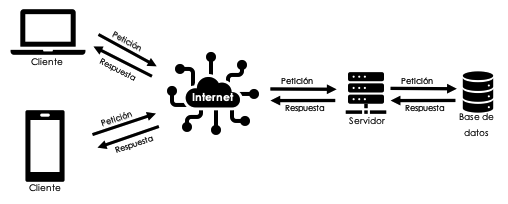
\includegraphics[width=13cm]{2-DefinicionDeLaArquitecturaTecnologica/arquitectura.png}
	\caption{Modelo cliente-servidor}
\end{figure}
Este modelo es el más básico y consiste en un cliente que se comunica con un servidor para acceder a los datos. En este caso, el cliente sería la aplicación, y el servidor sería el encargado de manejar la base de datos y la lógica de negocio.
Para implementarlo, es necesario realizar un análisis exhaustivo de las diferentes opciones tecnológicas disponibles para el desarrollo de la aplicación y para el servidor
\subsection{Aplicación web y móvil}
Para el desarrollo de esta aplicación hay varias alternativas. Entre ellas podemos destacar la realización de aplicaciones nativas, web apps o aplicaciones híbridas~\cite{nativas_vs_web_vs_hibridas}~\cite{web_vs_nativas_vs_hibridas}.
\subsubsection{Aplicaciones Nativas}
Las aplicaciones nativas se desarrollan específicamente para un sistema operativo concreto, utilizando su SDK correspondiente. Esto les permite acceder de manera óptima a las funcionalidades del dispositivo y ofrecen un alto rendimiento y una mejor experiencia de usuario. Por ejemplo, para iOS se utiliza Swift y para Android, Kotlin o Java son las opciones más comunes. La desventaja es que requieren un desarrollo separado para cada plataforma, lo que puede aumentar los costes y tiempos de desarrollo.
\subsubsection{Web Apps}
Las aplicaciones web se ejecutan en un navegador y están desarrolladas principalmente en HTML5, CSS y JavaScript. No necesitan ser instaladas en el dispositivo y son accesibles desde cualquier plataforma con acceso a internet. Son más económicas y rápidas de desarrollar en comparación con las aplicaciones nativas y funcionan en casi todos los dispositivos. Sin embargo, suelen depender de una buena conexión a internet y pueden no ofrecer la misma fluidez y acceso a funciones del dispositivo que una aplicación nativa.
\subsubsection{Aplicaciones Híbridas}
Las aplicaciones híbridas combinan elementos de las aplicaciones nativas y web. Se desarrollan utilizando tecnologías web pero se empaquetan dentro de un contenedor nativo, permitiéndoles acceder a las funcionalidades del dispositivo. Esto significa que se puede escribir el código una sola vez y adaptarlo a múltiples plataformas. Ejemplos notables de aplicaciones híbridas incluyen Instagram y Airbnb ~\cite{airbnb}. Sin embargo, su rendimiento es menor en comparación con las nativas y se pueden encontrar posibles complejidades cuando se requiere acceso a funcionalidades específicas del dispositivo.\\[1ex]
Sin embargo, es importante tener en cuenta que, a pesar de las ventajas en términos de desarrollo multiplataforma, el rendimiento de las aplicaciones híbridas puede ser menor en comparación con las puramente nativas y pueden surgir complejidades cuando se requiere acceso a funcionalidades específicas del dispositivo.\\[1ex]
Para facilitar el desarrollo de aplicaciones híbridas, existen varios frameworks que ofrecen un conjunto de herramientas y componentes reutilizables. Estos frameworks permiten a los desarrolladores centrarse en la lógica y funcionalidad de la aplicación, reduciendo el tiempo y esfuerzo necesario para desarrollar aplicaciones que funcionen en múltiples plataformas. A continuación, revisamos algunos de los frameworks más populares ~\cite{ionic_vs_native_vs_fluter}:
\begin{itemize}
	\item \textbf{Ionic:} Utiliza tecnologías web como HTML, CSS y JavaScript para construir aplicaciones móviles. Esto significa que puedes aprovechar tus habilidades web existentes y reutilizar código en diferentes plataformas. Ionic también cuenta con una robusta biblioteca de componentes de UI, gestos y herramientas para construir una aplicación con apariencia nativa.
	\item \textbf{React Native:} Utiliza tecnologías web pero compila el código a componentes nativos, por lo que el rendimiento y la experiencia son muy cercanos a los de una aplicación nativa. Tiene una gran colección de bibliotecas de terceros e integraciones. Sin embargo, puede ser más difícil de aprender en comparación con Ionic y Flutter. React Native también cuenta con el respaldo de Facebook, por lo que tiene una comunidad y un ecosistema fuertes.
	\item \textbf{Flutter:} Flutter utiliza el lenguaje de programación Dart de Google y widgets propietarios, y renderiza todo usando Skia, un motor de renderizado 2D. Esto permite que las aplicaciones de Flutter logren una apariencia y sensación nativas con alto rendimiento. Flutter es un framework relativamente nuevo, pero está creciendo rápidamente con una comunidad fuerte y muchas bibliotecas y plugins disponibles. Sin embargo, Dart puede tener una curva de aprendizaje más pronunciada para aquellos que vienen de los lenguajes web.
\end{itemize}
\subsection{Servidor}
En el desarrollo del backend, se dispone de una amplia gama de tecnologías que nos permiten construir y gestionar la lógica y los datos de nuestra aplicación.
\subsubsection{Framework y Entorno}
\begin{itemize}
	\item \textbf{Spring Boot:} Framework de Java muy valorado por su capacidad de simplificar el desarrollo de aplicaciones empresariales y microservicios. Ofrece autoconfiguración, una vasta colección de módulos y herramientas que permiten el desarrollo eficiente, y es compatible con diversas tecnologías de bases de datos tanto SQL como NoSQL. Su arquitectura basada en microservicios favorece la escalabilidad y flexibilidad, y su robusta documentación apoya a los desarrolladores a lo largo del proceso de desarrollo. Además, gracias a su naturaleza políglota y al soporte de la JVM, Spring Boot se integra bien con otros lenguajes de programación, ofreciendo una gran versatilidad para proyectos diversos~\cite{spring_boot_framework}.
	\item \textbf{NodeJS:} Entorno de ejecución que utiliza JavaScript para el desarrollo del backend. Es adecuado para un amplio rango de aplicaciones, desde aplicaciones en tiempo real, Internet de las Cosas (IoT) y aplicaciones basadas en REST API. NodeJS es reconocido por su eficiencia en el manejo de múltiples conexiones simultáneas, su capacidad para escalar aplicaciones, y por ser parte de un ecosistema rico en módulos y bibliotecas disponibles a través de NPM. Esto lo hace ideal para aplicaciones que requieren actualizaciones en tiempo real y para el desarrollo ágil y eficiente, manteniendo las operaciones no bloqueantes y basadas en eventos. Además, su comunidad de desarrollo activa y creciente ofrece un gran soporte y continua innovación~\cite{node_js}.
\end{itemize}
\subsubsection{Base de datos}
Tras elegir el framework y entorno adecuados para nuestro backend, es crucial seleccionar una base de datos que no solo se alinee con la naturaleza de nuestra aplicación, sino que también ofrezca el rendimiento, escalabilidad y fiabilidad necesarios. Las bases de datos son el pilar sobre el cual se estructuran, almacenan y acceden los datos esenciales para la funcionalidad de la aplicación.
\begin{itemize}
	\item \textbf{Relacional:} Es un tipo de base de datos que almacena y proporciona acceso a puntos de datos relacionados entre sí. Se basan en el modelo relacional, una forma intuitiva y directa de representar datos en tablas. Además, soportan transacciones ACID (Atomicidad, Consistencia, Aislamiento, Durabilidad), lo que garantiza que las operaciones de la base de datos se realicen de manera confiable y segura.\\
	      Sin embargo, las bases de datos relacionales pueden ser menos flexibles en términos de datos no estructurados o variables y es necesario añadir más potencia a un único servidor en caso de que aumente la demanda~\cite{sql}.
	\item \textbf{No relacional:} Es un tipo de base de datos que se caracteriza por su capacidad para almacenar y manejar grandes volúmenes de datos distribuidos, su esquema flexible y su escalabilidad horizontal. Hay muchos tipos de bases de datos, pero la que más se enfoca a este proyecto es la de documentos. En ella se asocia cada clave con una estructura de datos compleja llamada 'documento'. Estas bases de datos son idóneas para manejar datos semiestructurados y no estructurados ya que permiten una gran flexibilidad en la estructura de los datos almacenado. Algunos ejemplos de bases de datos de documentos son MongoDB~\cite{mongodb} y Couchbase~\cite{couchbase}.
	      Sin embargo, es importante considerar que las bases de datos NoSQL, a pesar de su escalabilidad y flexibilidad, pueden presentar desafíos en términos de consistencia de datos y complejidad de las consultas~\cite{nosql}.
\end{itemize}
\section{Selección de la arquitectura tecnológica}
Tras una exhaustiva evaluación de las distintas arquitecturas de aplicaciones móviles, se ha optado por el desarrollo de aplicaciones híbridas como la estrategia principal para este proyecto. Las aplicaciones híbridas, que integran las ventajas de las aplicaciones web y nativas, nos permiten escribir un único código base que es adaptable a múltiples plataformas, reduciendo significativamente el tiempo y los costos asociados con el desarrollo y mantenimiento en iOS y Android.\\[1ex]Hemos optado por la combinación de React e Ionic frente a otras alternativas como React Native y Flutter, basándonos en consideraciones estratégicas y en la experiencia previa del equipo. Si bien React Native es una poderosa solución para el desarrollo de aplicaciones móviles con capacidades para la web, su enfoque principal se centra en el desarrollo móvil. Sin embargo, la sinergia de React con Ionic se orienta específicamente hacia el desarrollo de aplicaciones híbridas desde su concepción, facilitando una experiencia de desarrollo unificada tanto para plataformas móviles como web. \\[1ex]La decisión de no elegir Flutter se basó principalmente en la curva de aprendizaje asociada con el dominio de Dart, el lenguaje de programación utilizado por Flutter, lo cual representa un desafío adicional para el equipo.\\[1ex]Para complementar nuestra elección de tecnologías frontend, hemos decidido adoptar un stack MERN~\cite{mern}. La integración de Node.js con Express.js para el desarrollo de nuestra API REST, junto con una base de datos NoSQL de documentos, ofrece una solución cohesiva y eficiente. Esta combinación no solo aprovecha la experiencia del equipo en tecnologías web, sino que también asegura una arquitectura escalable y flexible.
\input{3-EstudioDeViabilidadDelSistema/3-EstudioDeViabilidadDelSistema}
\chapter{Planificación y Gestión del TFG}
\section{Planificación del Proyecto}
\subsection{Identificación de Interesados}
Se identifican los siguientes grupos de interesados en el proyecto:
\begin{itemize}
	\item Turistas: como usuarios finales de la aplicación, su satisfacción y experiencia de uso es fundamental para el éxito del proyecto.
	\item Empresa: como la empresa que solicita la aplicación, espera obtener un producto de alta calidad que cumpla con sus requisitos y expectativas.
	\item Desarrolladores: los encargados de construir y mantener la aplicación, quienes necesitan especificaciones claras y un entorno de desarrollo bien definido.
	\item Proveedores de Servicios Tecnológicos: empresas o entidades que proporcionan infraestructura tecnológica, como servidores, servicios en la nube, etc.
	\item Autoridades Reguladoras: organismos que supervisan el cumplimiento de las leyes y regulaciones pertinentes, como la LOPD, RGPD y LSSI-CE.
	\item Comunidad Local: residentes y negocios locales que podrían beneficiarse indirectamente del incremento del turismo y la mejora de servicios.
\end{itemize}
\subsection{OBS y PBS}
\subsubsection*{Organizational Breackdown Structure}
La ``Organizational Breackdown Structure`` (OBS) es una representación jerárquica de la estructura organizativa del proyecto.
Define los roles y responsabilidades de los miembros del equipo del proyecto y sus relaciones.
La OBS ayuda a comprender la estructura de informes, los canales de comunicación y la coordinación entre los diferentes interesados del proyecto.
\\[1ex]
En la siguiente figura, se representa la OBS utilizando un diagrama de bloques. Cada bloque representa un rol o posición específica dentro del equipo del proyecto. Las lineas indican las relaciones de informe entre los roles.

\begin{figure}[H]
	\centering
	\begin{adjustwidth}{-0.55cm}{}
		\begin{tikzpicture}[
				scale=0.7, every node/.style={scale=0.7},
				node distance = 3mm and 0mm,
				block/.style = {draw, rectangle, minimum height=20mm, text width=30mm, align=center, fill=gray!25},
				line/.style = {draw, thick}
			]

			% Nodos
			\node [block] (consultor) {Consultor de tecnología};
			\node [block, right=of consultor] (analista) {Analista};
			\node [block, right=of analista] (arquitecto) {Arquitecto de software};
			\node [block, right=of arquitecto] (desarrollador) {Desarrollador Full-Stack};
			\node [block, right=of desarrollador] (admin) {Administrador de base de datos};
			\node [block, right=of admin] (disenador) {Diseñador de UX/UI};
			\node [block, right=of disenador] (devops) {DevOps};
			\node [block, right=of devops] (tester) {Tester};
			\node [block, right=of desarrollador, yshift=30mm, xshift=-15mm] (director) {Director de proyecto};
			% Líneas
			\draw [line] ([yshift=2.5mm, xshift=16.5mm] desarrollador.north) -- ([yshift=10mm, xshift=16.5mm]desarrollador.north) ;
			\draw [line] ([yshift=2mm] consultor.north) -- ([yshift=2mm]tester.north) ;
			\draw [line] ([yshift=0mm] consultor.north) -- ([yshift=2mm]consultor.north) ;
			\draw [line] ([yshift=0mm] analista.north) -- ([yshift=2mm]analista.north) ;
			\draw [line] ([yshift=0mm] arquitecto.north) -- ([yshift=2mm]arquitecto.north) ;
			\draw [line] ([yshift=0mm] desarrollador.north) -- ([yshift=2mm]desarrollador.north) ;
			\draw [line] ([yshift=0mm] admin.north) -- ([yshift=2mm]admin.north) ;
			\draw [line] ([yshift=0mm] disenador.north) -- ([yshift=2mm]disenador.north) ;
			\draw [line] ([yshift=0mm] devops.north) -- ([yshift=2mm]devops.north) ;
			\draw [line] ([yshift=0mm] tester.north) -- ([yshift=2mm]tester.north) ;
		\end{tikzpicture}
	\end{adjustwidth}
	\caption{Organizational Breackdown Structure (OBS)}
\end{figure}

\subsubsection*{Product Breackdown Structure}
La ``Product Breackdown Structure`` (PBS) es una herramienta utilizada en la gestión de proyectos para descomponer el producto final en componentes más pequeños y manejables.
\\ [1ex]
La PBS facilita la planificación, estimación de costos, asignación de recursos y seguimiento del progreso del proyecto. Cada componente de la PBS representa una funcionalidad o característica específica del producto y puede descomponerse en más subcomponentes.
\\ [1ex]
En la siguiente figura, se representa la PBS utilizando un diagrama de bloques. Cada bloque representa una fase del proyecto y sus actividades asociadas. Las lineas indican la secuencia de las fases del proyecto.

\tikzset{
	base/.style = {draw, text width=30mm, minimum height=20mm, align=center},
	fase/.style = {base, fill=gray!30, rectangle},
	actividad/.style = {base, fill=gray!10},
	linea/.style = {draw, thick}
}

\begin{figure}[H]
	\centering
	\begin{adjustwidth}{-0.45cm}{}
		\begin{tikzpicture}[scale=0.7, every node/.style={scale=0.7}, node distance=3mm and 3mm]
			% Fases
			\node[fase] (gestion) {Gestión inicial};
			\node[fase, right=of gestion] (analisis) {Análisis};
			\node[fase, right=of analisis] (diseno) {Diseño};
			\node[fase, right=of diseno] (implementacion) {Implementación};
			\node[fase, right=of implementacion] (pruebas) {Pruebas};
			\node[fase, right=of pruebas] (documentacion) {Documentación};
			\node[fase, right=of documentacion] (cierre) {Cierre de proyecto};
			\node[fase, right=of diseno, yshift=25mm] (proyecto) {Proyecto};
			% ... Otras fases

			% Actividades de Gestión Inicial
			\node[actividad, below=of gestion, xshift=2.5mm] (explicacion) {Explicación del proyecto};
			\node[actividad, below=of explicacion] (estudio) {Estudio de las alternativas tecnológicas};
			%\node[actividad, below=of estudio] (viabilidad) {Estudio de la viabilidad};
			\node[actividad, below=of estudio] (planificacion) {Planificación del proyecto};
			\node[actividad, below=of planificacion] (creacion) {Creación de un plan de gestion de riesgos};
			\node[actividad, below=of creacion] (riesgos) {Identificación de riesgos};
			\node[actividad, below=of riesgos] (pinicial) {Realización del presupuesto inicial};
			% Actividades de Análisis
			\node[actividad, below=of analisis, xshift=2.5mm] (definicion) {Definición del alcance del sistema};
			\node[actividad, below=of definicion] (requisitos) {Análisis de los requisitos};
			\node[actividad, below=of requisitos] (acasos) {Análisis de los casos de uso};
			\node[actividad, below=of acasos] (aclases) {Análisis de las clases};
			\node[actividad, below=of aclases] (prototipos) {Diseño de los prototipos de las interfaces de usuario};
			\node[actividad, below=of prototipos] (plan) {Elaboración del plan de pruebas};
			% Actividades de Diseño
			\node[actividad, below=of diseno, xshift=2.5mm] (dcasos) {Diseño de casos de uso};
			\node[actividad, below=of dcasos] (dclases) {Diseño de clases};
			\node[actividad, below=of dclases] (darquitectura) {Diseño de la arquitectura del sistema};
			\node[actividad, below=of darquitectura] (mbbdd) {Modelado de bases de datos};
			\node[actividad, below=of mbbdd] (inter) {Diseño de la interfaz de usuario};
			\node[actividad, below=of inter] (dpruebas) {Diseño de pruebas};
			% Actividades de Implementación
			\node[actividad, below=of implementacion, xshift=2.5mm] (repo) {Creación de los repositorios};
			\node[actividad, below=of repo] (server) {Creación del servidor de aplicaciones};
			\node[actividad, below=of server] (cliente) {Creación de la aplicación del cliente};
			\node[actividad, below=of cliente] (intebbdd) {Integración de la base de datos};
			\node[actividad, below=of intebbdd] (gusuarios) {Implementación del subsistema de gestión de usuarios};
			\node[actividad, below=of gusuarios] (gactividades) {Implementación del subsistema de gestión de actividades};
			\node[actividad, below=of gactividades] (greservas) {Implementación del subsistema de gestión de reservas};
			\node[actividad, below=of greservas] (pasarela) {Integración de la pasarela de pago};
			\node[actividad, below=of pasarela] (codeinter) {Codificación de estilos e interfaz de usuario};
			% Actividades de Pruebas
			\node[actividad, below=of pruebas, xshift=2.5mm] (uni) {Desarrollo de pruebas unitarias};
			\node[actividad, below=of uni] (inte) {Desarrollo de pruebas de integración};
			\node[actividad, below=of inte] (acces) {Desarrollo de pruebas de accesibilidad};

			%Documentación
			\node[actividad, below=of documentacion, xshift=2.5mm] (instalacion) {Manual de instalación};
			\node[actividad, below=of instalacion] (ejecucion) {Manual de ejecución};
			\node[actividad, below=of ejecucion] (musuario) {manual de usuario};

			%Cierre
			\node[actividad, below=of cierre, xshift=2.5mm] (planicierre) {Elaboración de la planificacion de cierre};
			\node[actividad, below=of planicierre] (preucierre) {Calculo del presupuesto final};
			\node[actividad, below=of preucierre] (reucierre) {Reunion de cierre};


			% Conexiones entre fases
			\draw[linea] ([yshift=2.5mm]gestion.north) -- ([yshift=2.5mm]cierre.north);
			\draw[linea] (gestion.north) -- +(0,3mm);
			\draw[linea] (analisis.north) -- +(0,3mm);
			\draw[linea] (diseno.north) -- +(0,3mm);
			\draw[linea] (implementacion.north) -- +(0,5mm);
			\draw[linea] (pruebas.north) -- +(0,3mm);
			\draw[linea] (documentacion.north) -- +(0,3mm);
			\draw[linea] (cierre.north) -- +(0,3mm);

			% Conexiones entre actividades
			\draw[linea] ([xshift=-16mm]gestion.south) -- ([xshift=-18.5mm,yshift=10mm]pinicial.south);
			\draw[linea] (explicacion.west) -- +(-2mm,0);
			\draw[linea] (estudio.west) -- +(-2mm,0);
			\draw[linea] (planificacion.west) -- +(-2mm,0);
			\draw[linea] (creacion.west) -- +(-2mm,0);
			\draw[linea] (riesgos.west) -- +(-2mm,0);
			\draw[linea] (pinicial.west) -- +(-2mm,0);

			\draw[linea] ([xshift=-16mm]analisis.south) -- ([xshift=-18.5mm,yshift=10mm]plan.south);
			\draw[linea] (definicion.west) -- +(-2mm,0);
			\draw[linea] (requisitos.west) -- +(-2mm,0);
			\draw[linea] (acasos.west) -- +(-2mm,0);
			\draw[linea] (aclases.west) -- +(-2mm,0);
			\draw[linea] (prototipos.west) -- +(-2mm,0);
			\draw[linea] (plan.west) -- +(-2mm,0);

			\draw[linea] ([xshift=-16mm]diseno.south) -- ([xshift=-18.5mm,yshift=10mm]dpruebas.south);
			\draw[linea] (dcasos.west) -- +(-2mm,0);
			\draw[linea] (dclases.west) -- +(-2mm,0);
			\draw[linea] (darquitectura.west) -- +(-2mm,0);
			\draw[linea] (mbbdd.west) -- +(-2mm,0);
			\draw[linea] (inter.west) -- +(-2mm,0);
			\draw[linea] (dpruebas.west) -- +(-2mm,0);

			\draw[linea] ([xshift=-16mm]implementacion.south) -- ([xshift=-18.5mm,yshift=10mm]codeinter.south);
			\draw[linea] (repo.west) -- +(-2mm,0);
			\draw[linea] (server.west) -- +(-2mm,0);
			\draw[linea] (cliente.west) -- +(-2mm,0);
			\draw[linea] (intebbdd.west) -- +(-2mm,0);
			\draw[linea] (gusuarios.west) -- +(-2mm,0);
			\draw[linea] (gactividades.west) -- +(-2mm,0);
			\draw[linea] (greservas.west) -- +(-2mm,0);
			\draw[linea] (pasarela.west) -- +(-2mm,0);
			\draw[linea] (codeinter.west) -- +(-2mm,0);

			\draw[linea] ([xshift=-16mm]pruebas.south) -- ([xshift=-18.5mm,yshift=10mm]acces.south);
			\draw[linea] (uni.west) -- +(-2mm,0);
			\draw[linea] (inte.west) -- +(-2mm,0);
			\draw[linea] (acces.west) -- +(-2mm,0);

			\draw[linea] ([xshift=-16mm]documentacion.south) -- ([xshift=-18.5mm,yshift=10mm]musuario.south);
			\draw[linea] (instalacion.west) -- +(-2mm,0);
			\draw[linea] (ejecucion.west) -- +(-2mm,0);
			\draw[linea] (musuario.west) -- +(-2mm,0);

			\draw[linea] ([xshift=-16mm]cierre.south) -- ([xshift=-18.5mm,yshift=10mm]reucierre.south);
			\draw[linea] (planicierre.west) -- +(-2mm,0);
			\draw[linea] (preucierre.west) -- +(-2mm,0);
			\draw[linea] (reucierre.west) -- +(-2mm,0);

		\end{tikzpicture}
	\end{adjustwidth}
	\caption{Product Breackdown Structure}
\end{figure}

\subsection{Planificación Inicial. WBS}
Se estima que se emplearán 640 horas para elaborar el proyecto, comenzando el día 1 de marzo de 2023 y finalizando el día 31 de mayo de 2023. Se trabajarían 49 horas semanales, es decir, 7 horas al día de lunes a domingo.\\[1ex]
La planificación se ha dividido en varias fases:
\begin{planificacion}
	\centering
	\begin{tabular}{ | m{9cm} | c | c | c |}
		\hline
		\textbf{Fase}      & \textbf{Duración (horas)} & \textbf{Comienzo} & \textbf{Fin} \\
		\hline
		Gestión inicial    & 63                        & 1/3/23            & 9/3/23       \\
		\hline
		Análisis           & 56                        & 10/3/23           & 17/3/23      \\
		\hline
		Diseño             & 113                       & 18/3/23           & 3/4/23       \\
		\hline
		Implementación     & 287                       & 3/4/23            & 14/5/23      \\
		\hline
		Pruebas            & 105                       & 14/5/23           & 29/5/23      \\
		\hline
		Documentación      & 11                        & 29/5/23           & 30/5/23      \\
		\hline
		Cierre de proyecto & 5                         & 30/5/23           & 31/5/23      \\
		\hline
	\end{tabular}
	\caption{Resumen de Fases y Cronograma del Proyecto}
\end{planificacion}

\subsubsection{Gestión inicial}
\begin{planificacion}
	\centering
	\begin{tabular}{ | m{9cm} | c | c | c |}
		\hline
		\textbf{Nombre de tarea}                  & \textbf{Duración (horas)} & \textbf{Comienzo} & \textbf{Fin} \\
		\hline
		Explicación del proyecto                  & 2                         & 1/3/23            & 1/3/23       \\
		\hline
		Estudio de las alternativas tecnológicas  & 10                        & 1/3/23            & 2/3/23       \\
		\hline
		Selección de la arquitectura tecnológica  & 5                         & 2/3/23            & 3/3/23       \\
		\hline
		Estudio de viabilidad                     & 15                        & 3/3/23            & 5/3/23       \\
		\hline
		Planificación del proyecto                & 10                        & 5/3/23            & 6/3/23       \\
		\hline
		Creación de un plan de gestión de riesgos & 8                         & 7/3/23            & 8/3/23       \\
		\hline
		Identificación de riesgos                 & 8                         & 8/3/23            & 9/3/23       \\
		\hline
		Realización del presupuesto inicial       & 5                         & 9/3/23            & 9/3/23       \\
		\hline
	\end{tabular}
	\caption{Detalle de Tareas y Cronograma de la Fase de Gestión Inicial}
\end{planificacion}

\subsubsection{Análisis}
\begin{planificacion}
	\centering
	\begin{tabular}{ | m{9cm} | c | c | c | }
		\hline
		\textbf{Nombre de la tarea}                           & \textbf{Duración (horas)} & \textbf{Comienzo} & \textbf{Fin} \\\hline
		Definición del alcance del sistema                    & 5                         & 10/3/23           & 10/3/23      \\\hline
		Análisis de los requisitos                            & 15                        & 10/3/23           & 12/3/23      \\\hline
		Análisis de los casos de uso                          & 15                        & 12/3/23           & 14/3/23      \\\hline
		Análisis de clases                                    & 8                         & 15/3/23           & 16/3/23      \\\hline
		Diseño de los prototipos de las interfaces de usuario & 5                         & 16/3/23           & 16/3/23      \\\hline
		Elaboración del plan de pruebas                       & 8                         & 16/3/23           & 17/3/23      \\\hline
	\end{tabular}
	\caption{Detalle de Tareas y Cronograma de la Fase de Análisis}
	\label{table:analysis_design_phase}
\end{planificacion}
\subsubsection{Diseño}
\input{4-PlanificacionYGestionDelTFG/PlanificacionInicial/TablaDiseño}
\subsubsection{Implementación}
\begin{planificacion}
	\centering
	\begin{tabular}{ | m{9cm} | c | c | c |}
		\hline
		\textbf{Nombre de la tarea}                             & \textbf{Duración (horas)} & \textbf{Comienzo} & \textbf{Fin} \\
		\hline
		Creación de los repositorios                            & 2                         & 3/4/23            & 3/4/23       \\
		\hline
		Creación del servidor de aplicaciones                   & 2                         & 3/4/23            & 3/4/23       \\
		\hline
		Creación de la aplicación cliente                       & 2                         & 3/4/23            & 3/4/23       \\
		\hline
		Integración de la base de datos                         & 5                         & 4/4/23            & 4/4/23       \\
		\hline
		Implementación del subsistema de gestión de usuarios    & 20                        & 4/4/23            & 7/4/23       \\
		\hline
		Implementación del subsistema de gestión de actividades & 30                        & 7/4/23            & 11/4/23      \\
		\hline
		Implementación del subsistema de gestión de reservas    & 100                       & 11/4/23           & 26/4/23      \\
		\hline
		Integración de pasarela de pago                         & 50                        & 26/4/23           & 3/5/23       \\
		\hline
		Codificación de estilos e interfaz de usuario           & 50                        & 3/5/23            & 10/5/23      \\
		\hline
		Despliegue del entorno                                  & 26                        & 10/5/23           & 14/5/23      \\
		\hline
	\end{tabular}
	\caption{Detalle de Tareas y Cronograma de la Fase de Implementación}
\end{planificacion}
\subsubsection{Pruebas}
\begin{planificacion}
	\centering
	\begin{tabular}{ | m{9cm} | c | c | c |}
		\hline
		\textbf{Nombre de la tarea}          & \textbf{Duración (horas)} & \textbf{Comienzo} & \textbf{Fin} \\
		\hline
		Desarrollo de pruebas unitarias      & 50                        & 14/5/23           & 21/5/23      \\
		\hline
		Desarrollo de pruebas de integración & 40                        & 21/5/23           & 26/5/23      \\
		\hline
		Desarrollo de pruebas de usabilidad  & 15                        & 27/5/23           & 29/5/23      \\
		\hline
	\end{tabular}
	\caption{Detalle de Tareas y Cronograma de la Fase de Pruebas}
\end{planificacion}

\subsubsection{Documentación}
\begin{planificacion}
	\centering
	\begin{tabular}{ | m{9cm} | c | c | c | }
		\hline
		\textbf{Nombre de la tarea} & \textbf{Duración (horas)} & \textbf{Comienzo} & \textbf{Fin} \\\hline
		Manual de instalación       & 2                         & 29/5/23           & 29/5/23      \\\hline
		Manual de ejecución         & 1                         & 29/5/23           & 30/5/23      \\\hline
		Manual de usuario           & 8                         & 29/5/23           & 30/5/23      \\\hline
	\end{tabular}
	\caption{Detalle de Tareas y Cronograma de la Fase de Documentación}
\end{planificacion}

\subsubsection{Cierre de Proyecto}
\begin{planificacion}
	\centering
	\begin{tabular}{ | m{9cm} | c | c | c | }
		\hline
		\textbf{Nombre de la tarea}           & \textbf{Duración (horas)} & \textbf{Comienzo} & \textbf{Fin} \\\hline
		Elaboración de la planificación final & 2                         & 30/5/23           & 30/5/23      \\\hline
		Cálculo del presupuesto final         & 2                         & 31/5/23           & 31/5/23      \\\hline
		Reunión de cierre del proyecto        & 1                         & 31/5/23           & 31/5/23      \\\hline
	\end{tabular}
	\caption{Detalle de Tareas y Cronograma de la Fase de Cierre del Proyecto}
\end{planificacion}

\subsubsection{Diagrama de Gantt}

\begin{figure}[H]
	\centering
	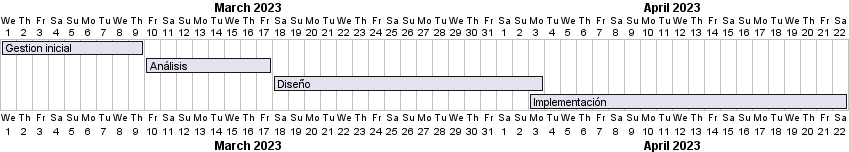
\includegraphics[width=1\textwidth]{4-PlanificacionYGestionDelTFG/PlanificacionInicial/gant1.png}
	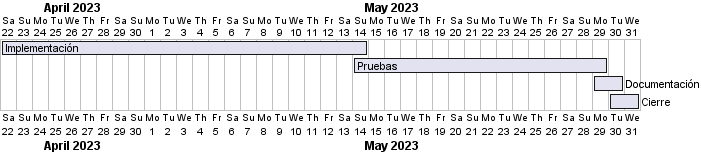
\includegraphics[width=0.8\textwidth]{4-PlanificacionYGestionDelTFG/PlanificacionInicial/gant2.png}
	\caption{Diagrama de Gantt de la planificación inicial del proyecto}
\end{figure}

\begin{figure}[H]
	\centering
	\begin{minipage}{0.45\textwidth}
		\includegraphics[width=1\textwidth]{4-PlanificacionYGestionDelTFG/PlanificacionInicial/gant-gestionInicial.png}
		\caption{Diagrama de Gantt de la fase de gestión inicial}
	\end{minipage}
	\hfill
	\begin{minipage}{0.45\textwidth}
		\centering
		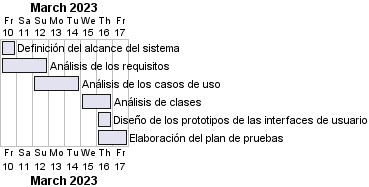
\includegraphics[width=1\textwidth]{4-PlanificacionYGestionDelTFG/PlanificacionInicial/gant-analisis.png}
		\caption{Diagrama de Gantt de la fase de análisis}
	\end{minipage}
\end{figure}

\begin{figure}[H]
	\centering
	\includegraphics[width=0.6\textwidth]{4-PlanificacionYGestionDelTFG/PlanificacionInicial/gant-diseño.png}
	\caption{Diagrama de Gantt de la fase de diseño}
\end{figure}

\begin{figure}[H]
	\centering
	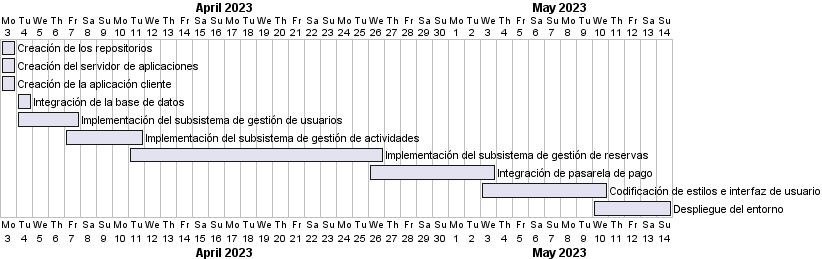
\includegraphics[width=1\textwidth]{4-PlanificacionYGestionDelTFG/PlanificacionInicial/gant-implementacion.png}
	\caption{Diagrama de Gantt de la fase de implementación}
\end{figure}

\begin{figure}[H]
	\centering
	\begin{minipage}{0.65\textwidth}
		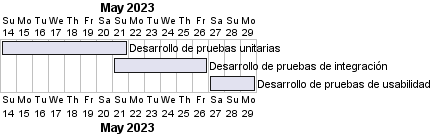
\includegraphics[width=1\textwidth]{4-PlanificacionYGestionDelTFG/PlanificacionInicial/gant-pruebas.png}
		\caption{Diagrama de Gantt de la fase de pruebas}
	\end{minipage}
	\hfill
	\begin{minipage}{0.25\textwidth}
		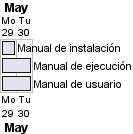
\includegraphics[width=1\textwidth]{4-PlanificacionYGestionDelTFG/PlanificacionInicial/gant-documentacion.png}
		\caption{Diagrama de Gantt de la fase de documentación}
	\end{minipage}
\end{figure}

\begin{figure}[H]
	\centering
	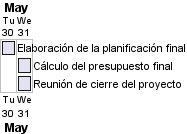
\includegraphics[width=0.4\textwidth]{4-PlanificacionYGestionDelTFG/PlanificacionInicial/gant-cierre.png}
	\caption{Diagrama de Gantt de la fase de cierre de proyecto}
\end{figure}
\subsection{Riesgos}
\subsubsection{Plan de Gestión de Riesgos}
El contenido del plan de gestión de riesgos se desarrolla en el \textit{Apéndice \ref{appendix:plan-gestion-riesgos}. Plan de gestión de riesgos}.
\subsubsection{Identificación de Riesgos}
\begin{table}[H]
	\centering
	\begin{tabular}{|c|m{4cm}|m{10cm}|}
		\hline
		{\textbf{ID}} & {\textbf{Nombre del riesgo}} & {\textbf{Descripción}}                                                                                                                                               \\
		\hline
		R1            & Problemas de compatibilidad  & Puede haber problemas de compatibilidad con las diferentes versiones de los navegadores o dispositivos móviles                                                       \\
		\hline
		R2            & Cambios de requisitos        & Puede haber una escasez de recursos como presupuesto, tiempo y equipos de desarrollo adecuados, lo que puede afectar la calidad y la eficiencia del proyecto         \\
		\hline
		R3            & Problemas de seguridad       & La aplicación puede estar expuesta a vulnerabilidades de seguridad que pueden ser explotadas por atacantes malintencionados.                                         \\
		\hline
		R4            & Falta de pruebas adecuadas   & La falta de pruebas adecuadas puede llevar a la liberación de una aplicación con errores y problemas de rendimientos.                                                \\
		\hline
		R5            & Problemas de rendimiento     & La aplicación puede ser lenta o ineficiente debido a problemas de diseño o codificación.                                                                             \\
		\hline
		R6            & Fallos de integración        & Puede haber problemas al integrar diferentes componentes y sistemas de la aplicación.                                                                                \\
		\hline
		R7            & Falta de experiencia         & La falta de experiencia en el equipo de desarrollo puede afectar la calidad del código y la capacidad para resolver problemas complejos.                             \\
		\hline
		R8            & Errores de estimación        & Puede haber errores de estimación en cuanto a la duración y los recursos necesarios para completar el proyecto que pueden afectar la planificación y el presupuesto. \\
		\hline
		R9            & Problemas de comunicación    & La falta de comunicación o una mala comunicación entre los miembros del equipo o con los clientes puede llevar a malentendidos y errores.                            \\
		\hline
		R10           & Problemas de calidad         & Puede haber problemas de calidad en el código, la documentación o los procesos de desarrollo que pueden afectar la fiabilidad y la estabilidad de la aplicación.     \\
		\hline
	\end{tabular}
	\caption{Tabla de riesgos identificados}
\end{table}
\subsubsection{Registro de Riesgos}
Se incluirán los riesgos detallados en el \textit{Apéndice \ref{appendix:hojas-riesgos}. Hojas de riesgos}. Especificando tanto su impacto como su probabilidad.
\subsection{Presupuesto Inicial}
En esta sección se presentan las tarifas por hora estimadas para cada perfil profesional que se utilizarán para calcular los costos del proyecto.
Los precios por hora se han calculado tomando como referencia los salarios base anuales de cada perfil, de acuerdo con datos del mercado actual \cite{manfred2023}.
\begin{planificacion}
	\centering
	\begin{tabular}{ | m{9cm} | c | }
		\hline
		\textbf{Perfil}                & \textbf{Precio/hora} \\\hline
		Consultor de tecnología        & 35,55€               \\\hline
		Analista                       & 31,72€               \\\hline
		Arquitecto de software         & 36,65€               \\\hline
		Desarrollador Full-Stack       & 21,88€               \\\hline
		Arquitecto de software         & 27,30€               \\\hline
		Administrador de base de datos & 31,72€               \\\hline
		Diseñador de UX/UI             & 25,71€               \\\hline
		DevOps                         & 21,88€               \\\hline
		Tester                         & 16,41€               \\\hline
		Director de proyecto           & 33,91€               \\\hline
	\end{tabular}
	\caption{Presupuesto por perfil profesional}
\end{planificacion}

Los datos de las tarifas por hora han sido calculados a partir de los salarios base anuales de cada perfil.
A continuación, se detalla la referencia salarial utilizada para cada perfil:
\begin{itemize}
	\item  \textbf{Desarrollador Full-Stack:} 40.000€ anuales.
	\item  \textbf{Arquitecto de software:} 67.000€ anuales.
	\item  \textbf{Diseñador de UX/UI:} 47.000€ anuales.
	\item  \textbf{Tester:} 30.000€ anuales.
	\item  \textbf{Administrador de base de datos:} 58.000€ anuales.
	\item  \textbf{Analista:} 58.000€ anuales.
	\item  \textbf{Director de proyecto:} 62.000€ anuales.
	\item  \textbf{DevOps:} 40.000€ anuales.
	\item  \textbf{Consultor de tecnología:} 65.000€ anuales.
\end{itemize}
El precio por hora se ha calculado considerando una jornada laboral anual de 1.828 horas.
\subsubsection{Presupuesto de costes}
Para una mejor planificación y control del presupuesto del proyecto, se ha dividido el coste en varias fases.
Cada fase del proyecto representa un conjunto de actividades y entregables específicos.
A continuación, se presenta un desglose detallado de los costes asociados a cada fase del proyecto.
\\[1ex]
Este desglose permite identificar de manera clara y precisa los recursos necesarios y los costes estimados en cada etapa, facilitando así la gestión y asignación de los recursos a lo largo del ciclo de vida del proyecto.
\begin{planificacion}
	\centering
	\begin{tabular}{ | m{8.5cm} | c | m{2.5cm} |  m{1.5cm} |}
		\hline
		\textbf{Nombre de tarea}                  & \textbf{Duración(horas)} & \textbf{Perfil}         & \textbf{Precio} \\\hline
		Explicación del proyecto                  & 2                        & Director de proyecto    & 67,82€          \\\hline
		Estudio de las alternativas tecnológicas  & 10                       & Consultor de tecnología & 355,50€         \\\hline
		Selección de la arquitectura tecnológica  & 5                        & Arquitecto de software  & 183,25€         \\\hline
		Estudio de viabilidad                     & 15                       & Analista                & 475,80€         \\\hline
		Planificación del proyecto                & 10                       & Director de proyecto    & 339,10€         \\\hline
		Creación de un plan de gestión de riesgos & 8                        & Consultor de tecnología & 284,40€         \\\hline
		Identificación de riesgos                 & 8                        & Consultor de tecnología & 284,40€         \\\hline
	\end{tabular}
	\caption{Presupuesto inicial de la fase de gestión inicial}
\end{planificacion}

\begin{planificacion}
	\centering
	\begin{tabular}{ | m{8.5cm} | c | m{2.5cm} |  m{1.5cm} |}
		\hline
		\textbf{Nombre de la tarea}                           & \textbf{Duración(horas)} & \textbf{Perfil}    & \textbf{Precio} \\\hline
		Definición del alcance del sistema                    & 5                        & Analista           & 158,60€         \\\hline
		Análisis de los requisitos                            & 15                       & Analista           & 475,80€         \\\hline
		Análisis de los casos de uso                          & 15                       & Analista           & 475,80€         \\\hline
		Análisis de clases                                    & 8                        & Analista           & 253,76€         \\\hline
		Diseño de los prototipos de las interfaces de usuario & 5                        & Diseñador de UX/UI & 128,55€         \\\hline
		Elaboración del plan de pruebas                       & 8                        & Tester             & 131,28€         \\\hline
	\end{tabular}
	\caption{Presupuesto inicial de la fase de análisis}
\end{planificacion}

\begin{planificacion}
	\centering
	\begin{tabular}{ | m{8.5cm} | c | m{2.5cm} |  m{1.5cm} |}
		\hline
		\textbf{Nombre de la tarea}                      & \textbf{Duración(horas)} & \textbf{Perfil}                & \textbf{Precio} \\\hline
		Diseño de casos de uso reales                    & 15                       & Arquitecto de software         & 549,75€         \\\hline
		Diseño de clases                                 & 10                       & Arquitecto de software         & 366,50€         \\\hline
		Diseño de la arquitectura de módulos del sistema & 8                        & Arquitecto de software         & 293,20€         \\\hline
		Modelado de bases de datos                       & 5                        & Administrador de base de datos & 158,60€         \\\hline
		Diseño de la interfaz de usuario                 & 50                       & Diseñador de UX/UI             & 1285,50€        \\\hline
		Diseño de pruebas                                & 25                       & Tester                         & 410,25€         \\\hline
	\end{tabular}
	\caption{Presupuesto inicial de la fase de diseño}
\end{planificacion}

\begin{planificacion}
	\centering
	\begin{tabular}{ | m{8.5cm} | c | m{2.5cm} |  m{1.5cm} |}
		\hline
		\textbf{Nombre de la tarea}                             & \textbf{Duración(horas)} & \textbf{Perfil}                & \textbf{Precio} \\\hline
		Creación de los repositorios                            & 2                        & DevOps                         & 43,76€          \\\hline
		Creación del servidor de aplicaciones                   & 2                        & DevOps                         & 43,76€          \\\hline
		Creación de la aplicación cliente                       & 2                        & Desarrollador Full-Stack       & 43,76€          \\\hline
		Integración de la base de datos                         & 5                        & Administrador de base de datos & 158,60€         \\\hline
		Implementación del subsistema de gestión de usuarios    & 20                       & Desarrollador Full-Stack       & 437,60€         \\\hline
		Implementación del subsistema de gestión de actividades & 30                       & Desarrollador Full-Stack       & 656,40€         \\\hline
		Implementación del subsistema de gestión de reservas    & 100                      & Desarrollador Full-Stack       & 2188,00€        \\\hline
		Integración de pasarela de pago                         & 50                       & Desarrollador Full-Stack       & 1094,00€        \\\hline
		Codificación de estilos e interfaz de usuario           & 50                       & Diseñador de UX/UI             & 1285,50€        \\\hline
		Despliegue del entorno                                  & 26                       & DevOps                         & 568,88€         \\\hline
	\end{tabular}
	\caption{Presupuesto inicial de la fase de implementación}
\end{planificacion}

\begin{planificacion}
	\centering
	\begin{tabular}{ | m{8.5cm} | c | m{2.5cm} |  m{1.5cm} |}
		\hline
		\textbf{Nombre de la tarea}          & \textbf{Duración(horas)} & \textbf{Perfil} & \textbf{Precio} \\\hline
		Desarrollo de pruebas unitarias      & 50                       & Tester          & 820,50€         \\\hline
		Desarrollo de pruebas de integración & 40                       & Tester          & 656,40€         \\\hline
		Desarrollo de pruebas de usabilidad  & 15                       & Tester          & 246,15€         \\\hline
	\end{tabular}
	\caption{Presupuesto inicial de la fase de pruebas}
\end{planificacion}

\begin{planificacion}
	\centering
	\begin{tabular}{ | m{8.5cm} | c | m{2.5cm} |  m{1.5cm} |}
		\hline
		\textbf{Nombre de la tarea} & \textbf{Duración(horas)} & \textbf{Perfil}          & \textbf{Precio} \\\hline
		Manual de instalación       & 2                        & Desarrollador Full-Stack & 43,76€          \\\hline
		Manual de ejecución         & 1                        & Desarrollador Full-Stack & 21,88€          \\\hline
		Manual de usuario           & 8                        & Diseñador de UX/UI       & 205,68€         \\\hline
	\end{tabular}
	\caption{Presupuesto inicial de la fase de documentación}
\end{planificacion}

\begin{planificacion}
	\centering
	\begin{tabular}{ | m{8.5cm} | c | m{2.5cm} |  m{1.5cm} |}
		\hline
		\textbf{Nombre de la tarea}           & \textbf{Duración(horas)} & \textbf{Perfil}      & \textbf{Precio} \\\hline
		Elaboración de la planificación final & 2                        & Director de proyecto & 67,82€          \\\hline
		Cálculo del presupuesto final         & 2                        & Director de proyecto & 67,82€          \\\hline
		Reunión de cierre del proyecto        & 1                        & Director de proyecto & 33,91€          \\\hline
	\end{tabular}
	\caption{Presupuesto inicial de la fase de cierre de proyecto}
\end{planificacion}
\subsubsection{Presupuesto total de costes}
En esta sección se presenta una visión global del presupuesto total del proyecto, sumando los costes desglosados por fases y perfiles profesionales.
El objetivo es proporcionar una estimación completa y detallada de los recursos financieros necesarios para llevar a cabo el proyecto de principio a fin.

\begin{planificacion}
	\centering
	\begin{tabular}{ | m{9cm} | c | c |}
		\hline
		\textbf{Fase}      & \textbf{Duración (horas)} & \textbf{Precio}    \\\hline
		Gestión inicial    & 63                        & 2148,87€           \\\hline
		Análisis           & 56                        & 1623,79€           \\\hline
		Diseño             & 113                       & 3063,85€           \\\hline
		Implementación     & 287                       & 6410,00€           \\\hline
		Pruebas            & 105                       & 1722,45€           \\\hline
		Documentación      & 11                        & 271,32€            \\\hline
		Cierre de proyecto & 5                         & 169,55€            \\\hline
		\textbf{Total}     & \textbf{640}              & \textbf{15809,83€} \\\hline
	\end{tabular}
	\caption{Presupuesto de costes total}
\end{planificacion}

\subsubsection{Presupuesto de cliente}
Se ha seleccionado un margen del 20\% de beneficio basándonos en un análisis exhaustivo de los costos y las prácticas estándar de la industria.
Este margen permite cubrir adecuadamente los costos directos e indirectos, así como los riesgos asociados al desarrollo del proyecto, como posibles retrasos y cambios en los requisitos.
\\[1ex]
Además, al mantener un margen del 20\%, podemos ofrecer un precio competitivo que añade valor al cliente, asegurando la viabilidad financiera y la sostenibilidad a largo plazo del proyecto sin imponer un costo excesivo.
Este equilibrio entre rentabilidad y accesibilidad es esencial para fomentar la confianza del cliente y apoyar el crecimiento futuro de la empresa.

\begin{planificacion}
	\centering
	\begin{tabular}{ | m{9cm} | c | c |}
		\hline
		\textbf{Fase}      & \textbf{Duración (horas)} & \textbf{Precio }   \\\hline
		Gestión inicial    & 63                        & 2578,64€           \\\hline
		Análisis           & 56                        & 1948,55€           \\\hline
		Diseño             & 113                       & 3676,62€           \\\hline
		Implementación     & 287                       & 7692,00€           \\\hline
		Pruebas            & 105                       & 2066,94€           \\\hline
		Documentación      & 11                        & 325,58€            \\\hline
		Cierre de proyecto & 5                         & 203,46€            \\\hline
		\textbf{Total}     & \textbf{640}              & \textbf{18991,79€} \\\hline
	\end{tabular}
	\caption{Presupuesto para el cliente}
\end{planificacion}


\section{Ejecución del proyecto}
\subsection{Bitácora de incidencias}
Se ha llevado un registro de las incidencias que han surgido durante el desarrollo del proyecto, así como su impacto en la planificación del mismo. A continuación, se muestra una tabla con las incidencias registradas y su efecto en la planificación del proyecto.
\begin{table}[H]
	\centering
	\begin{tabular}{ | c |  c | c | m{4.7cm} | m{4.3cm} | }
		\hline
		\textbf{ID} & \textbf{Fecha de creación} & \textbf{Fecha de cierre} & \textbf{Descripción de la incidencia}                                                          & \textbf{Efecto en la planificación}                                     \\
		\hline
		1           & 10/3/23                    & 13/6/23                  & Cambio del jefe de proyecto                                                                    & Retraso de 3 meses en la revisión de la planificación del proyecto      \\
		\hline
		2           & 1/7/23                     & 3/6/24                   & Asignación de un proyecto adicional al equipo, requiriendo redistribución de recursos y tiempo & Reducción de la jornada de trabajo de 7 horas a 2 horas y media diarias \\
		\hline
		3           & 27/9/23                    & 16/10/23                 & Problema con la subida de imágenes al servidor                                                 & Retraso de 49 horas en la implementación del subsistema de actividades  \\
		\hline
		4           & 25/3/24                    & 29/3/24                  & Problemas en el despliegue del servidor con AWS y Docker durante la fase de implementación     & Retraso de 10 horas en la puesta en marcha del entorno de despliegue    \\
		\hline
	\end{tabular}
	\caption{Registro de Incidencias y su Impacto en la Planificación del Proyecto}
\end{table}

\subsection{Riesgos}
A continuación, se presentan los riesgos identificados en la planificación del proyecto, así como su seguimiento a lo largo del desarrollo del mismo. Para cada riesgo se proporciona una descripción, el retraso causado y el evento de bitácora asociado.
\begin{table}[H]
	\centering
	\begin{tabular}{ | c | m{13cm} | }
		\hline
		{\textbf{R9}}               & {Problemas de comunicación}                                                                                         \\
		\hline
		\textbf{Descripción}        & Cambio del jefe de proyecto, lo que causó un retraso significativo en la revisión de la planificación del proyecto. \\
		\hline
		\textbf{Retraso}            & 3 meses                                                                                                             \\
		\hline
		\textbf{Evento de bitácora} & 1                                                                                                                   \\
		\hline
	\end{tabular}
	\caption{Seguimiento del riesgo de cambio del jefe de proyecto}
\end{table}

\vspace{0.5cm}

\begin{table}[H]
	\centering
	\begin{tabular}{ | c | m{13cm} | }
		\hline
		{\textbf{R8}}               & {Errores de estimación}                                                                                                                                                   \\
		\hline
		\textbf{Descripción}        & Asignación de un proyecto adicional al equipo, requiriendo una redistribución significativa de recursos y tiempo. Esto resultó en una reducción de la jornada de trabajo. \\
		\hline
		\textbf{Retraso}            & Reducción de la jornada de trabajo de 7 horas a 2 horas y media diarias                                                                                                   \\
		\hline
		\textbf{Evento de bitácora} & 2                                                                                                                                                                         \\
		\hline
	\end{tabular}
	\caption{Seguimiento del riesgo de redistribución de recursos y tiempo}
\end{table}

\vspace{0.5cm}

\begin{table}[H]
	\centering
	\begin{tabular}{ | c | m{13cm} | }
		\hline
		{\textbf{R6}}               & {Fallos de integración}                                                                                    \\
		\hline
		\textbf{Descripción}        & Problema con la subida de imágenes al servidor, afectando la implementación del subsistema de actividades. \\
		\hline
		\textbf{Retraso}            & 49 horas                                                                                                   \\
		\hline
		\textbf{Evento de bitácora} & 3                                                                                                          \\
		\hline
	\end{tabular}
	\caption{Seguimiento del riesgo de problemas de integración}
\end{table}

\vspace{0.5cm}

\begin{table}[H]
	\centering
	\begin{tabular}{ | c | m{13cm} | }
		\hline
		{\textbf{R7}}               & {Falta de experiencia}                                                                      \\
		\hline
		\textbf{Descripción}        & Problemas en el despliegue del servidor con AWS y Docker durante la fase de implementación. \\
		\hline
		\textbf{Retraso}            & 10 horas                                                                                    \\
		\hline
		\textbf{Evento de bitácora} & 4                                                                                           \\
		\hline
	\end{tabular}
	\caption{Seguimiento del riesgo de problemas en el despliegue del servidor}
\end{table}

\section{Cierre del Proyecto}
\subsection{Planificación Final}
Se estima que se emplearon 699 horas para elaborar el proyecto, comenzando el día 1 de marzo de
2023 y finalizando el día 3 de junio de 2024.
La planificación se ha dividido en varias fases:
\begin{planificacion}
	\centering
	\begin{tabular}{ | m{9cm} | c | c | c |}
		\hline
		\textbf{Fase}      & \textbf{Duración (horas)} & \textbf{Comienzo} & \textbf{Fin} \\
		\hline
		Gestión inicial    & 63                        & 1/3/23            & 9/3/23       \\
		\hline
		Análisis           & 56                        & 13/6/23           & 22/6/23      \\
		\hline
		Diseño             & 113                       & 22/6/23           & 4/8/23       \\
		\hline
		Implementación     & 346                       & 7/8/23            & 29/3/24      \\
		\hline
		Pruebas            & 105                       & 1/4/24            & 28/5/24      \\
		\hline
		Documentación      & 11                        & 28/5/24           & 31/5/24      \\
		\hline
		Cierre de proyecto & 5                         & 31/5/24           & 3/6/24       \\
		\hline
	\end{tabular}
	\caption{Resumen de Fases y Cronograma del Proyecto}
\end{planificacion}

\subsubsection{Gestion Inicial}
\begin{planificacion}
	\centering
	\begin{tabular}{ | m{9cm} | c | c | c |}
		\hline
		\textbf{Nombre de tarea}                  & \textbf{Duración (horas)} & \textbf{Comienzo} & \textbf{Fin} \\
		\hline
		Explicación del proyecto                  & 2                         & 1/3/23            & 1/3/23       \\
		\hline
		Estudio de las alternativas tecnológicas  & 10                        & 1/3/23            & 2/3/23       \\
		\hline
		Selección de la arquitectura tecnológica  & 5                         & 2/3/23            & 3/3/23       \\
		\hline
		Estudio de viabilidad                     & 15                        & 3/3/23            & 5/3/23       \\
		\hline
		Planificación del proyecto                & 10                        & 5/3/23            & 6/3/23       \\
		\hline
		Creación de un plan de gestión de riesgos & 8                         & 7/3/23            & 8/3/23       \\
		\hline
		Identificación de riesgos                 & 8                         & 8/3/23            & 9/3/23       \\
		\hline
	\end{tabular}
	\caption{Detalle de Tareas y Cronograma de la Fase de Gestión Inicial}
\end{planificacion}

\subsubsection{Analisis}
\begin{planificacion}
	\centering
	\begin{tabular}{ | m{9cm} | c | c | c | }
		\hline
		\textbf{Nombre de la tarea}                           & \textbf{Duración (horas)} & \textbf{Comienzo} & \textbf{Fin} \\\hline
		Definición del alcance del sistema                    & 5                         & 13/6/23           & 13/6/23      \\\hline
		Análisis de los requisitos                            & 15                        & 13/6/23           & 15/6/23      \\\hline
		Análisis de los casos de uso                          & 15                        & 15/6/23           & 19/6/23      \\\hline
		Análisis de clases                                    & 8                         & 19/6/23           & 20/6/23      \\\hline
		Diseño de los prototipos de las interfaces de usuario & 5                         & 20/6/23           & 20/6/23      \\\hline
		Elaboración del plan de pruebas                       & 8                         & 21/6/23           & 22/6/23      \\\hline
	\end{tabular}
	\caption{Detalle de Tareas y Cronograma de la Fase de Análisis}
	\label{table:analysis_design_phase}
\end{planificacion}
\subsubsection{Diseño}
\input{4-PlanificacionYGestionDelTFG/PlanificacionFinal/TablaDiseño}
\subsubsection{Implementación}
\begin{planificacion}
	\centering
	\begin{tabular}{ | m{9cm} | c | c | c |}
		\hline
		\textbf{Nombre de la tarea}                             & \textbf{Duración (horas)} & \textbf{Comienzo} & \textbf{Fin} \\
		\hline
		Creación de los repositorios                            & 2                         & 7/8/23            & 7/8/23       \\
		\hline
		Creación del servidor de aplicaciones                   & 2                         & 8/8/23            & 8/8/23       \\
		\hline
		Creación de la aplicación cliente                       & 2                         & 9/8/23            & 9/8/23       \\
		\hline
		Integración de la base de datos                         & 5                         & 10/8/23           & 12/8/23      \\
		\hline
		Implementación del subsistema de gestión de usuarios    & 20                        & 14/8/23           & 24/8/23      \\
		\hline
		Implementación del subsistema de gestión de actividades & 79                        & 25/8/23           & 16/10/23     \\
		\hline
		Implementación del subsistema de gestión de reservas    & 100                       & 17/10/23          & 28/12/23     \\
		\hline
		Integración de pasarela de pago                         & 50                        & 29/12/23          & 23/1/24      \\
		\hline
		Codificación de estilos e interfaz de usuario           & 50                        & 24/1/24           & 16/2/24      \\
		\hline
		Despliegue del entorno                                  & 36                        & 19/2/24           & 29/3/24      \\
		\hline
	\end{tabular}
	\caption{Detalle de Tareas y Cronograma de la Fase de Implementación}
\end{planificacion}
\subsubsection{Pruebas}
\begin{planificacion}
	\centering
	\begin{tabular}{ | m{9cm} | c | c | c |}
		\hline
		\textbf{Nombre de la tarea}          & \textbf{Duración (horas)} & \textbf{Comienzo} & \textbf{Fin} \\
		\hline
		Desarrollo de pruebas unitarias      & 50                        & 1/4/24            & 24/4/24      \\
		\hline
		Desarrollo de pruebas de integración & 40                        & 25/4/24           & 17/5/24      \\
		\hline
		Desarrollo de pruebas de usabilidad  & 15                        & 20/5/24           & 28/5/24      \\
		\hline
	\end{tabular}
	\caption{Detalle de Tareas y Cronograma de la Fase de Pruebas}
\end{planificacion}

\subsubsection{Documentación}
\begin{planificacion}
	\centering
	\begin{tabular}{ | m{9cm} | c | c | c | }
		\hline
		\textbf{Nombre de la tarea} & \textbf{Duración (horas)} & \textbf{Comienzo} & \textbf{Fin} \\\hline
		Manual de instalación       & 2                         & 28/5/24           & 29/5/24      \\\hline
		Manual de ejecución         & 1                         & 29/5/24           & 29/5/24      \\\hline
		Manual de usuario           & 8                         & 29/5/24           & 31/5/24      \\\hline
	\end{tabular}
	\caption{Detalle de Tareas y Cronograma de la Fase de Documentación}
\end{planificacion}

\subsubsection{Cierre de Proyecto}
\begin{planificacion}
	\centering
	\begin{tabular}{ | m{9cm} | c | c | c | }
		\hline
		\textbf{Nombre de la tarea}           & \textbf{Duración (horas)} & \textbf{Comienzo} & \textbf{Fin} \\\hline
		Elaboración de la planificación final & 2                         & 31/5/24           & 31/5/24      \\\hline
		Cálculo del presupuesto final         & 2                         & 3/6/24            & 3/6/24       \\\hline
		Reunión de cierre del proyecto        & 1                         & 3/6/24            & 3/6/24       \\\hline
	\end{tabular}
	\caption{Detalle de Tareas y Cronograma de la Fase de Cierre del Proyecto}
\end{planificacion}

\subsubsection{Diagrama de Gantt}
\begin{figure}[H]
	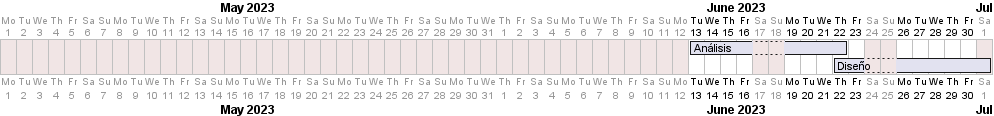
\includegraphics[width=0.01\textwidth]{4-PlanificacionYGestionDelTFG/PlanificacionFinal/gantt/gant2.png}
	\vspace{0.4cm}
	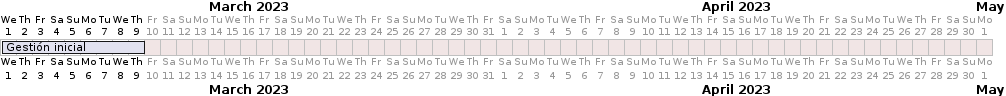
\includegraphics[width=1\textwidth]{4-PlanificacionYGestionDelTFG/PlanificacionFinal/gantt/gant1.png}
	\vspace{0.4cm}
	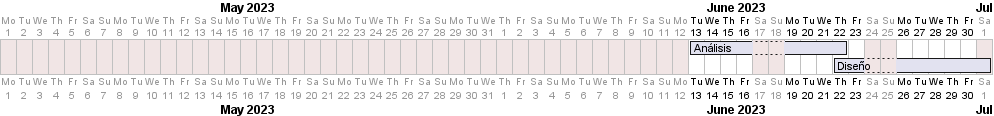
\includegraphics[width=1\textwidth]{4-PlanificacionYGestionDelTFG/PlanificacionFinal/gantt/gant2.png}
	\vspace{0.4cm}
	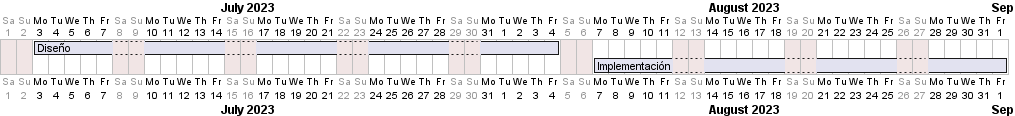
\includegraphics[width=1\textwidth]{4-PlanificacionYGestionDelTFG/PlanificacionFinal/gantt/gant3.png}
	\vspace{0.4cm}
	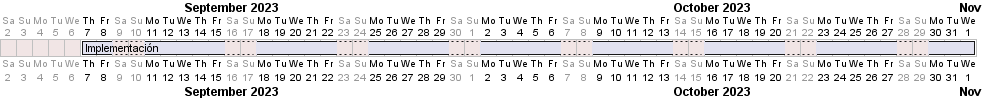
\includegraphics[width=1\textwidth]{4-PlanificacionYGestionDelTFG/PlanificacionFinal/gantt/gant4.png}
	\vspace{0.4cm}
	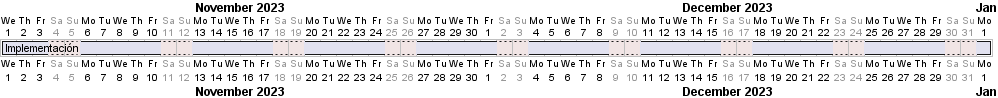
\includegraphics[width=1\textwidth]{4-PlanificacionYGestionDelTFG/PlanificacionFinal/gantt/gant5.png}
	\vspace{0.4cm}
	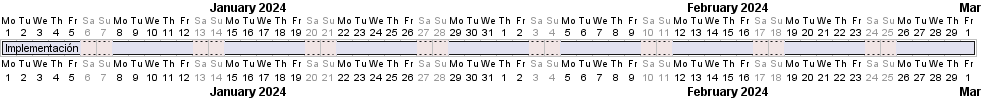
\includegraphics[width=1\textwidth]{4-PlanificacionYGestionDelTFG/PlanificacionFinal/gantt/gant6.png}
	\vspace{0.4cm}
	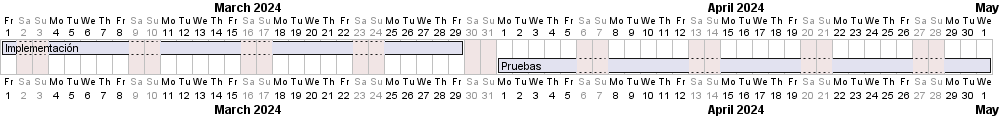
\includegraphics[width=1\textwidth]{4-PlanificacionYGestionDelTFG/PlanificacionFinal/gantt/gant7.png}
	\vspace{0.4cm}
	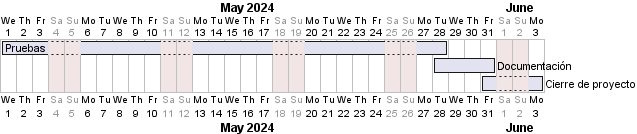
\includegraphics[width=0.6\textwidth]{4-PlanificacionYGestionDelTFG/PlanificacionFinal/gantt/gant8.png}
	\caption{Diagrama de Gantt de la planificación del TFG}
\end{figure}

\begin{figure}[H]
	\centering
	\begin{minipage}{0.45\textwidth}
		\includegraphics[width=0.8\textwidth]{4-PlanificacionYGestionDelTFG/PlanificacionFinal/gantt/gant-gestionInicial.png}
		\caption{Diagrama de Gantt de la fase de gestión inicial}
	\end{minipage}
	\hfill
	\begin{minipage}{0.45\textwidth}
		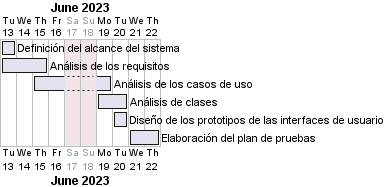
\includegraphics[width=1\textwidth]{4-PlanificacionYGestionDelTFG/PlanificacionFinal/gantt/gant-analisis.png}
		\caption{Diagrama de Gantt de la fase de análisis}
	\end{minipage}
\end{figure}

\begin{figure}[H]
	\includegraphics[width=1\textwidth]{4-PlanificacionYGestionDelTFG/PlanificacionFinal/gantt/gant-diseño.png}
	\caption{Diagrama de Gantt de la fase de diseño}
\end{figure}

\begin{figure}[H]
	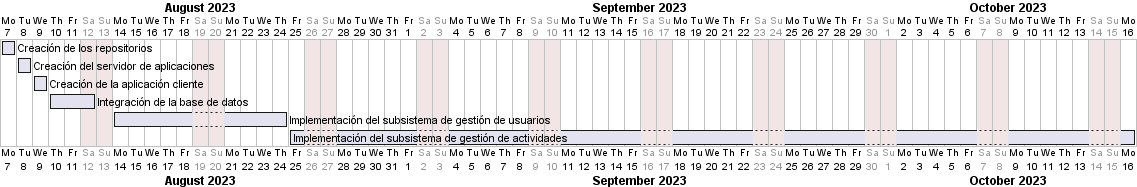
\includegraphics[width=0.01\textwidth]{4-PlanificacionYGestionDelTFG/PlanificacionFinal/gantt/gant-implementacion1.png}
	\vspace{0.4cm}
	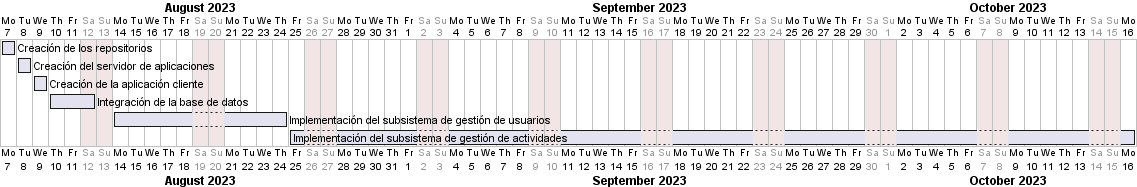
\includegraphics[width=1\textwidth]{4-PlanificacionYGestionDelTFG/PlanificacionFinal/gantt/gant-implementacion1.png}
	\vspace{0.4cm}
	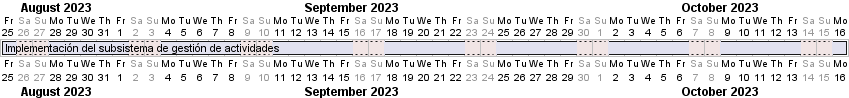
\includegraphics[width=1\textwidth]{4-PlanificacionYGestionDelTFG/PlanificacionFinal/gantt/gant-implementacion2.png}
	\vspace{0.4cm}
	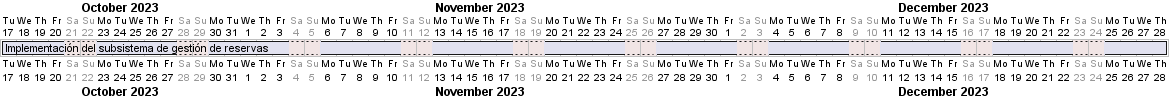
\includegraphics[width=1\textwidth]{4-PlanificacionYGestionDelTFG/PlanificacionFinal/gantt/gant-implementacion3.png}
	\vspace{0.4cm}
	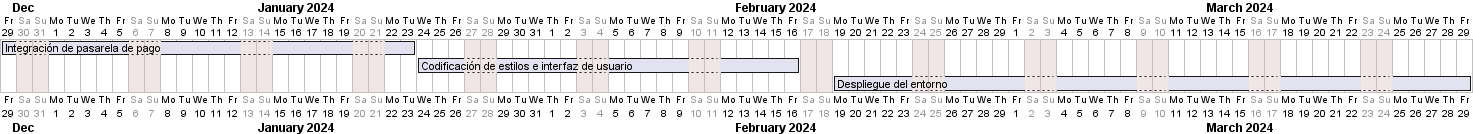
\includegraphics[width=1\textwidth]{4-PlanificacionYGestionDelTFG/PlanificacionFinal/gantt/gant-implementacion4.png}
	\caption{Diagrama de Gantt de la fase de implementación}
\end{figure}

\begin{figure}[H]
	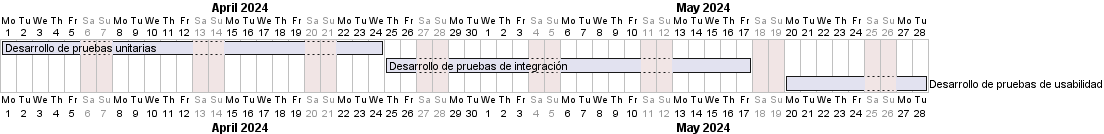
\includegraphics[width=1\textwidth]{4-PlanificacionYGestionDelTFG/PlanificacionFinal/gantt/gant-pruebas.png}
	\caption{Diagrama de Gantt de la fase de pruebas}
\end{figure}

\begin{figure}[H]
	\centering
	\begin{minipage}{0.45\textwidth}
		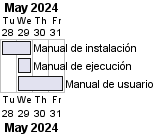
\includegraphics[width=0.5\textwidth]{4-PlanificacionYGestionDelTFG/PlanificacionFinal/gantt/gant-documentacion.png}
		\caption{Diagrama de Gantt de la fase de documentación}
	\end{minipage}
	\hfill
	\begin{minipage}{0.45\textwidth}
		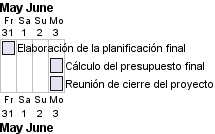
\includegraphics[width=0.6\textwidth]{4-PlanificacionYGestionDelTFG/PlanificacionFinal/gantt/gant-cierre.png}
		\caption{Diagrama de Gantt de la fase de cierre}
	\end{minipage}
\end{figure}

\subsection{Presupuesto Final}
\subsubsection{Presupuesto de costes}
Este es el presupuesto final del proyecto. A continuación, se presenta un desglose detallado de los costes asociados a cada fase del proyecto.
\\[1ex]
Este desglose permite identificar de manera clara y precisa los recursos y costes que ha tenido cada fase.
\begin{planificacion}
	\centering
	\begin{tabular}{ | m{8.5cm} | c | m{2.5cm} |  m{1.5cm} |}
		\hline
		\textbf{Nombre de tarea}                  & \textbf{Duración(horas)} & \textbf{Perfil}         & \textbf{Precio} \\\hline
		Explicación del proyecto                  & 2                        & Director de proyecto    & 67,82€          \\\hline
		Estudio de las alternativas tecnológicas  & 10                       & Consultor de tecnología & 355,50€         \\\hline
		Selección de la arquitectura tecnológica  & 5                        & Arquitecto de software  & 183,25€         \\\hline
		Estudio de viabilidad                     & 15                       & Analista                & 475,80€         \\\hline
		Planificación del proyecto                & 10                       & Director de proyecto    & 339,10€         \\\hline
		Creación de un plan de gestión de riesgos & 8                        & Consultor de tecnología & 284,40€         \\\hline
		Identificación de riesgos                 & 8                        & Consultor de tecnología & 284,40€         \\\hline
	\end{tabular}
	\caption{Presupuesto final de la fase de gestión inicial}
\end{planificacion}

\begin{planificacion}
	\centering
	\begin{tabular}{ | m{8.5cm} | c | m{2.5cm} |  m{1.5cm} |}
		\hline
		\textbf{Nombre de la tarea}                           & \textbf{Duración(horas)} & \textbf{Perfil}    & \textbf{Precio} \\\hline
		Definición del alcance del sistema                    & 5                        & Analista           & 158,60€         \\\hline
		Análisis de los requisitos                            & 15                       & Analista           & 475,80€         \\\hline
		Análisis de los casos de uso                          & 15                       & Analista           & 475,80€         \\\hline
		Análisis de clases                                    & 8                        & Analista           & 253,76€         \\\hline
		Diseño de los prototipos de las interfaces de usuario & 5                        & Diseñador de UX/UI & 128,55€         \\\hline
		Elaboración del plan de pruebas                       & 8                        & Tester             & 131,28€         \\\hline
	\end{tabular}
	\caption{Presupuesto final de la fase de análisis}
\end{planificacion}

\begin{planificacion}
	\centering
	\begin{tabular}{ | m{8.5cm} | c | m{2.5cm} |  m{1.5cm} |}
		\hline
		\textbf{Nombre de la tarea}                      & \textbf{Duración(horas)} & \textbf{Perfil}                & \textbf{Precio} \\\hline
		Diseño de casos de uso reales                    & 15                       & Arquitecto de software         & 549,75€         \\\hline
		Diseño de clases                                 & 10                       & Arquitecto de software         & 366,50€         \\\hline
		Diseño de la arquitectura de módulos del sistema & 8                        & Arquitecto de software         & 293,20€         \\\hline
		Modelado de bases de datos                       & 5                        & Administrador de base de datos & 158,60€         \\\hline
		Diseño de la interfaz de usuario                 & 50                       & Diseñador de UX/UI             & 1285,50€        \\\hline
		Diseño de pruebas                                & 25                       & Tester                         & 410,25€         \\\hline
	\end{tabular}
	\caption{Presupuesto final de la fase de diseño}
\end{planificacion}

\begin{planificacion}
	\centering
	\begin{tabular}{ | m{8.5cm} | c | m{2.5cm} |  m{1.5cm} |}
		\hline
		\textbf{Nombre de la tarea}                             & \textbf{Duración(horas)} & \textbf{Perfil}                & \textbf{Precio} \\\hline
		Creación de los repositorios                            & 2                        & DevOps                         & 43,76€          \\\hline
		Creación del servidor de aplicaciones                   & 2                        & DevOps                         & 43,76€          \\\hline
		Creación de la aplicación cliente                       & 2                        & Desarrollador Full-Stack       & 43,76€          \\\hline
		Integración de la base de datos                         & 5                        & Administrador de base de datos & 158,60€         \\\hline
		Implementación del subsistema de gestión de usuarios    & 20                       & Desarrollador Full-Stack       & 437,60€         \\\hline
		Implementación del subsistema de gestión de actividades & 79                       & Desarrollador Full-Stack       & 1.728,52€       \\\hline
		Implementación del subsistema de gestión de reservas    & 100                      & Desarrollador Full-Stack       & 2188,00€        \\\hline
		Integración de pasarela de pago                         & 50                       & Desarrollador Full-Stack       & 1094,00€        \\\hline
		Codificación de estilos e interfaz de usuario           & 50                       & Diseñador de UX/UI             & 1285,50€        \\\hline
		Despliegue del entorno                                  & 36                       & DevOps                         & 787,68€         \\\hline
	\end{tabular}
	\caption{Presupuesto final de la fase de implementación}
\end{planificacion}

\begin{planificacion}
	\centering
	\begin{tabular}{ | m{8.5cm} | c | m{2.5cm} |  m{1.5cm} |}
		\hline
		\textbf{Nombre de la tarea}          & \textbf{Duración(horas)} & \textbf{Perfil} & \textbf{Precio} \\\hline
		Desarrollo de pruebas unitarias      & 50                       & Tester          & 820,50€         \\\hline
		Desarrollo de pruebas de integración & 40                       & Tester          & 656,40€         \\\hline
		Desarrollo de pruebas de usabilidad  & 15                       & Tester          & 246,15€         \\\hline
	\end{tabular}
	\caption{Presupuesto final de la fase de pruebas}
\end{planificacion}

\begin{planificacion}
	\centering
	\begin{tabular}{ | m{8.5cm} | c | m{2.5cm} |  m{1.5cm} |}
		\hline
		\textbf{Nombre de la tarea} & \textbf{Duración(horas)} & \textbf{Perfil}          & \textbf{Precio} \\\hline
		Manual de instalación       & 2                        & Desarrollador Full-Stack & 43,76€          \\\hline
		Manual de ejecución         & 1                        & Desarrollador Full-Stack & 21,88€          \\\hline
		Manual de usuario           & 8                        & Diseñador de UX/UI       & 205,68€         \\\hline
	\end{tabular}
	\caption{Presupuesto final de la fase de documentación}
\end{planificacion}

\begin{planificacion}
	\centering
	\begin{tabular}{ | m{8.5cm} | c | m{2.5cm} |  m{1.5cm} |}
		\hline
		\textbf{Nombre de la tarea}           & \textbf{Duración(horas)} & \textbf{Perfil}      & \textbf{Precio} \\\hline
		Elaboración de la planificación final & 2                        & Director de proyecto & 67,82€          \\\hline
		Cálculo del presupuesto final         & 2                        & Director de proyecto & 67,82€          \\\hline
		Reunión de cierre del proyecto        & 1                        & Director de proyecto & 33,91€          \\\hline
	\end{tabular}
	\caption{Presupuesto final de la fase de cierre de proyecto}
\end{planificacion}
\subsubsection{Presupuesto total de costes}
En esta sección se presenta una visión global del presupuesto total del proyecto, sumando los costes desglosados por fases y perfiles profesionales.
Como podemos ver en la tabla, el coste total del proyecto asciende a 16652,96€, distribuido en las distintas fases del proyecto. Gracias a ese 20\% de margen de beneficio que se ha añadido al presupuesto inicial, se ha conseguido que el proyecto no se haya excedido del presupuesto inicialmente establecido y además se obtenga un beneficio de 2775,49€.
\begin{planificacion}
	\centering
	\begin{tabular}{ | m{9cm} | c | c |}
		\hline
		\textbf{Fase}      & \textbf{Duración (horas)} & \textbf{Precio}    \\\hline
		Gestión inicial    & 63                        & 2148,87€           \\\hline
		Análisis           & 56                        & 1623,79€           \\\hline
		Diseño             & 113                       & 3063,85€           \\\hline
		Implementación     & 287                       & 7811,18€           \\\hline
		Pruebas            & 105                       & 1723,05€           \\\hline
		Documentación      & 11                        & 271,32€            \\\hline
		Cierre de proyecto & 5                         & 169,55€            \\\hline
		\textbf{Total}     & \textbf{669}              & \textbf{16652,96€} \\\hline
	\end{tabular}
	\caption{Presupuesto de costes total}
\end{planificacion}

\subsection{Informe de lecciones aprendidas}
\begin{itemize}
	\item La comunicación clara y constante con los stakeholders es fundamental para entender correctamente sus necesidades y expectativas
	\item Las estimaciones iniciales a menudo son optimistas y no consideran imprevistos. Habría que incorporar un margen de tiempo adicional para enfrentar posibles imprevistos y revisar las estimaciones con expertos de la materia.
	\item Los riesgos no identificados pueden afectar seriamente al progreso del proyecto.
\end{itemize}

\chapter{Análisis del Sistema de Información}
\section{Determinación del Alcance del Sistema}
El sistema consistirá en una aplicación móvil y web que brindará una amplia selección de tours y actividades para el disfrute de los turistas en la región de Asturias. Los usuarios tendrán la capacidad de buscar y reservar actividades, así como de gestionar sus reservas previamente realizadas.\\[1ex]
Además, el sistema facilitará que los usuarios valoren el servicio recibido y dejen reseñas. Por otro lado, la aplicación ofrecerá a la empresa de turismo una herramienta de administración para agregar y gestionar sus actividades y usuarios\\[1ex]
El alcance del sistema estará limitado a las funcionalidades mencionadas. No se contempla la inclusión de características adicionales, como la reserva de alojamiento o la compra de billetes de avión, dado que estas están fuera del ámbito del sistema y su integración requeriría de complejas conexiones con otros sistemas.
\section{Establecimiento de Requisitos}
\subsection{Obtención de los Requisitos del Sistema}
\subsubsection{Requisitos funcionales}
\paragraph{Registro de usuario}
\begin{enumitem}[label=\bfseries{RReg \arabic*.},leftmargin=*]
	\item El sistema permitirá a cualquier usuario registrarse.
	\begin{enumitem}[label*=\bfseries{\arabic*.}]
		\item El sistema requerirá que se rellenen los siguientes campos obligatorios.
		\begin{enumitem}[label*=\bfseries{\arabic*.}]
			\item Nombre y apellidos del usuario.
			\begin{enumitem}[label*=\bfseries{\arabic*.}]
				\item El sistema comprobará que la cadena introducida es mayor o igual que 8.
			\end{enumitem}
			\item Dirección de correo electrónico.
			\begin{enumitem}[label*=\bfseries{\arabic*.}]
				\item El sistema comprobará que coincide con un patrón de correo electrónico.
				\item El sistema comprobará que ese correo electrónico no ha sido registrado por otro usuario.
			\end{enumitem}
			\item Contraseña.
			\begin{enumitem}[label*=\bfseries{\arabic*.}]
				\item El sistema comprobará que la contraseña introducida tiene una longitud mínima de 8 y máxima de 16.
			\end{enumitem}
			\item Confirmación de Contraseña.
			\begin{enumitem}[label*=\bfseries{\arabic*.}]
				\item El sistema comprobará que la confirmación coincida con la contraseña introducida anteriormente.
			\end{enumitem}
		\end{enumitem}
		\item El sistema tendrá los siguientes campos opcionales.
		\begin{enumitem}[label*=\bfseries{\arabic*.}]
			\item País.
			\item Teléfono.
			\begin{enumitem}[label*=\bfseries{\arabic*.}]
				\item El sistema comprobará que el número de teléfono introducido es valido.
			\end{enumitem}
			\item Fecha de nacimiento.
			\begin{enumitem}[label*=\bfseries{\arabic*.}]
				\item El sistema comprobará que el formato de la fecha de nacimiento es correcto.
				\item El sistema comprobará que la fecha de nacimiento introducida es posterior al día de hoy
			\end{enumitem}
		\end{enumitem}
		\item Al completar todos los campos obligatorios, el sistema habilitará un botón para confirmar el registro.
		\begin{enumitem}[label*=\bfseries{\arabic*.}]
			\item El sistema comprobará que los datos introducidos en los campos están rellenos correctamente.
			\begin{enumitem}[label*=\bfseries{\arabic*.}]
				\item El sistema mostrará un mensaje de error si no se cumple alguna de las comprobaciones de los campos.
				\item En caso de cumplir todas las comprobaciones, el sistema guardará los datos de registro.
				\begin{enumitem}[label*=\bfseries{\arabic*.}]
					\item El sistema autenticará al usuario con los datos registrados automáticamente.
					\item El sistema mostrará la pantalla principal.
				\end{enumitem}
			\end{enumitem}
		\end{enumitem}
	\end{enumitem}
\end{enumitem}

\paragraph{Inicio de sesión}
\begin{enumitem}[label=\bfseries{RIni \arabic*.},leftmargin=*]
	\item El sistema permitirá a un usuario iniciar sesión.
	\begin{enumitem}[label*=\bfseries{\arabic*.}]
		\item El sistema requerirá que se rellenen unos campos obligatorios.
		\begin{enumitem}[label*=\bfseries{\arabic*.}]
			\item Dirección de correo electrónico.
			\begin{enumitem}[label*=\bfseries{\arabic*.}]
				\item El sistema comprobará que coincide con un patrón de correo electrónico.
			\end{enumitem}
			\item Contraseña.
			\begin{enumitem}[label*=\bfseries{\arabic*.}]
				\item El sistema comprobará que la contraseña introducida tiene una longitud mínima de 8 y máxima de 16.
			\end{enumitem}
		\end{enumitem}
		\item Al completar todos los campos, el sistema deberá habilitar un botón para confirmar el inicio de sesión.
		\begin{enumitem}[label*=\bfseries{\arabic*.}]
			\item Al confirmar el inicio de sesión, el sistema comprobará que los datos introducidos en los campos cumplen con sus comprobaciones individuales.
			\begin{enumitem}[label*=\bfseries{\arabic*.}]
				\item El sistema mostrará un mensaje de error si no se cumple alguna de las comprobaciones de los campos.
				\item En caso de cumplir con todas las comprobaciones, el sistema comprobará que las credenciales introducidas en los campos coinciden con algún usuario registrado.
				\begin{enumitem}[label*=\bfseries{\arabic*.}]
					\item El sistema mostrará un mensaje de error si no existe ningún usuario asociado a esas credenciales.
					\item En caso de existir un usuario asociado, el sistema mostrará un mensaje de que el usuario ha iniciado sesión correctamente.
				\end{enumitem}
			\end{enumitem}
		\end{enumitem}
	\end{enumitem}
\end{enumitem}

\paragraph{Perfil de usuario}
\begin{enumitem}[label=\bfseries{RPer \arabic*.},leftmargin=*]
	\item El sistema permitirá a los usuarios registrados visualizar su perfil.
	\begin{enumitem}[label*=\bfseries{\arabic*.}]
		\item El sistema mostrará los datos registrados por el usuario.
	\end{enumitem}
	\item El sistema permitirá a los usuarios registrados modificar datos de su perfil.
	\begin{enumitem}[label*=\bfseries{\arabic*.}]
		\item El sistema permitirá modificar los siguientes campos.
		\begin{enumitem}[label*=\bfseries{\arabic*.}]
			\item Nombre y Apellidos.
			\begin{enumitem}[label*=\bfseries{\arabic*.}]
				\item El sistema comprobará que la cadena introducida es mayor o igual que 8.
			\end{enumitem}
			\item Dirección de correo electrónico.
			\begin{enumitem}[label*=\bfseries{\arabic*.}]
				\item El sistema comprobará que coincide con un patrón de correo electrónico.
				\item El sistema comprobará que ese correo electrónico no ha sido registrado por otro usuario.
			\end{enumitem}
			\item Fecha de nacimiento.
			\begin{enumitem}[label*=\bfseries{\arabic*.}]
				\item El sistema comprobará que el formato de la fecha de nacimiento es correcto.
				\item El sistema comprobará que la fecha de nacimiento introducida es posterior al día de hoy.
			\end{enumitem}
			\item Teléfono.
			\begin{enumitem}[label*=\bfseries{\arabic*.}]
				\item El sistema comprobará que el número de teléfono introducido es valido.
			\end{enumitem}
			\item País.
		\end{enumitem}
		\item El sistema permitirá cancelar la edición de perfil.
		\item Al editar algún campo, el sistema deberá habilitar un botón para confirmar el guardado.
		\begin{enumitem}[label*=\bfseries{\arabic*.}]
			\item El sistema comprobará que los campos cumplen con sus comprobaciones individuales.
			\begin{enumitem}[label*=\bfseries{\arabic*.}]
				\item El sistema mostrará un mensaje de error si no se cumple alguna de las comprobaciones de los campos.
				\item En caso de cumplir con todas las comprobaciones, el sistema mostrará un mensaje de que el usuario ha actualizado correctamente sus datos.
			\end{enumitem}
		\end{enumitem}
	\end{enumitem}

	\item El sistema permitirá que cualquier usuario registrado elimine su cuenta.
	\begin{enumitem}[label*=\bfseries{\arabic*.}]
		\item El sistema mostrará un mensaje de confirmación.
	\end{enumitem}
	\item El sistema permitirá a los usuarios registrados cambiar su contraseña.
	\begin{enumitem}[label*=\bfseries{\arabic*.}]
		\item El sistema requerirá que el usuario introduzca su contraseña actual.
		\begin{enumitem}[label*=\bfseries{\arabic*.}]
			\item El sistema comprobará que la contraseña introducida coincide con la contraseña actual del usuario.
		\end{enumitem}
		\item El sistema requerirá que el usuario introduzca la nueva contraseña.
		\begin{enumitem}[label*=\bfseries{\arabic*.}]
			\item El sistema comprobará que la contraseña introducida tiene una longitud mínima de 8 y máxima de 16.
		\end{enumitem}
		\item El sistema requerirá que el usuario confirme la nueva contraseña.
		\begin{enumitem}[label*=\bfseries{\arabic*.}]
			\item El sistema comprobará que la confirmación coincide con la nueva contraseña introducida anteriormente.
		\end{enumitem}
		\item Al completar todos los campos, el sistema habilitará un botón para confirmar el cambio de contraseña.
		\begin{enumitem}[label*=\bfseries{\arabic*.}]
			\item El sistema comprobará que los datos introducidos en los campos están rellenos correctamente.
			\begin{enumitem}[label*=\bfseries{\arabic*.}]
				\item El sistema mostrará un mensaje de error si no se cumple alguna de las comprobaciones de los campos.
				\item En caso de cumplir todas las comprobaciones, el sistema mostrará un mensaje de que el usuario ha actualizado correctamente su contraseña.
			\end{enumitem}
		\end{enumitem}
	\end{enumitem}
	\item El sistema permitirá a los usuarios registrados cerrar sesión.
\end{enumitem}


\paragraph{Listado de actividades}
\begin{enumitem}[label=\bfseries{RLis \arabic*.},leftmargin=*,]
	\item El sistema permitirá a cualquiera listar todas las actividades disponibles.
	\item El sistema no permitirá visualizar la información de las actividades deshabilitadas.
	\item El sistema permitirá a cualquiera visualizar la información de las actividades activas o canceladas temporalmente.
	\begin{enumitem}[label*=\bfseries{\arabic*.}]
		\item Nombre.
		\item Localidad.
		\item Duración.
		\item Idiomas disponibles.
		\item Descripción.
		\item Precios.
		\item Horarios.
	\end{enumitem}
\end{enumitem}

\paragraph{Usuario administrador}
\begin{enumitem}[label=\bfseries{RAdm \arabic*.},leftmargin=*]
	\item El sistema permitirá a todos los usuarios con rol de administrador eliminar cuentas.
	\begin{enumitem}[label*=\bfseries{\arabic*.}]
		\item El sistema no permitirá que se eliminen todas las cuentas de administradores.
		\item El sistema mostrará un mensaje de confirmación.
	\end{enumitem}
	\item El sistema permitirá a los usuarios con rol de administrador crear cuentas.
	\begin{enumitem}[label*=\bfseries{\arabic*.}]
		\item El sistema requerirá que se rellenen los siguientes campos obligatorios.
		\begin{enumitem}[label*=\bfseries{\arabic*.}]
			\item Nombre y apellidos del usuario.
			\begin{enumitem}[label*=\bfseries{\arabic*.}]
				\item El sistema comprobará que la cadena introducida es mayor o igual que 8.
			\end{enumitem}
			\item Dirección de correo electrónico.
			\begin{enumitem}[label*=\bfseries{\arabic*.}]
				\item El sistema comprobará que coincide con un patrón de correo electrónico.
				\item El sistema comprobará que ese correo electrónico no ha sido registrado por otro usuario.
			\end{enumitem}
			\item Contraseña.
			\begin{enumitem}[label*=\bfseries{\arabic*.}]
				\item El sistema comprobará que la contraseña introducida tiene una longitud mínima de 8 y máxima de 16.
			\end{enumitem}
			\item Rol.
			\begin{enumitem}[label*=\bfseries{\arabic*.}]
				\item El sistema proporcionará una lista de roles predefinidos.
				\begin{enumitem}[label*=\bfseries{\arabic*.}]
					\item Administrador.
					\item Guía.
					\item Usuario.
				\end{enumitem}
			\end{enumitem}
		\end{enumitem}
		\item El sistema tendrá los siguientes campos opcionales.
		\begin{enumitem}[label*=\bfseries{\arabic*.}]
			\item País.
			\item Teléfono.
			\begin{enumitem}[label*=\bfseries{\arabic*.}]
				\item El sistema comprobará que el número de teléfono introducido es valido.
			\end{enumitem}
			\item Fecha de nacimiento.
			\begin{enumitem}[label*=\bfseries{\arabic*.}]
				\item El sistema comprobará que el formato de la fecha de nacimiento es correcto.
				\item El sistema comprobará que la fecha de nacimiento introducida es posterior al día de hoy
			\end{enumitem}
		\end{enumitem}
		\item Al completar todos los campos obligatorios, el sistema habilitará un botón para confirmar el registro.
		\begin{enumitem}[label*=\bfseries{\arabic*.}]
			\item El sistema comprobará que los datos introducidos en los campos están rellenos correctamente.
			\begin{enumitem}[label*=\bfseries{\arabic*.}]
				\item El sistema mostrará un mensaje de error si no se cumple alguna de las comprobaciones de los campos.
				\item En caso de cumplir todas las comprobaciones, el sistema guardará los datos de registro.
			\end{enumitem}
		\end{enumitem}
		\item El sistema permitirá cancelar la creación de cuenta.
	\end{enumitem}
	\item El sistema permitirá a los usuarios con rol de administrador listar todos los usuarios registrados.
	\begin{enumitem}[label*=\bfseries{\arabic*.}]
		\item El sistema permitirá hacer búsquedas aplicando o no algún filtro.
		\begin{enumitem}[label*=\bfseries{\arabic*.}]
			\item Búsquedas por Nombre.
			\item Búsquedas por Apellidos.
			\item Búsquedas por Dirección de correo electrónico.
			\item Filtrar por Rol.
		\end{enumitem}
	\end{enumitem}
	\item El sistema permitirá a los usuarios con rol de administrador visualizar los datos de un usuario buscado.
	\begin{enumitem}[label*=\bfseries{\arabic*.}]
		\item Nombre y Apellidos.
		\item Dirección de correo electrónico.
		\item Rol.
		\item Fecha de nacimiento.
		\item País.
		\item Teléfono.
		\item Lista de reservas realizadas.
		\begin{enumitem}[label*=\bfseries{\arabic*.}]
			\item Fecha.
			\item Nombre de la actividad.
			\item Localidad.
			\item Estado de la reserva.
			\item Número de plazas.
			\item Precio.
		\end{enumitem}
	\end{enumitem}
	\item El sistema permitirá a los usuarios con rol de administrador editar información de un usuario buscado.
	\begin{enumitem}[label*=\bfseries{\arabic*.}]
		\item El sistema permitirá modificar los siguientes campos.
		\begin{enumitem}[label*=\bfseries{\arabic*.}]
			\item Nombre y Apellidos.
			\begin{enumitem}[label*=\bfseries{\arabic*.}]
				\item El sistema comprobará que la cadena introducida es mayor o igual que 8.
			\end{enumitem}
			\item Dirección de correo electrónico.
			\begin{enumitem}[label*=\bfseries{\arabic*.}]
				\item El sistema comprobará que coincide con un patrón de correo electrónico.
				\item El sistema comprobará que ese correo electrónico no ha sido registrado por otro usuario.
			\end{enumitem}
			\item Fecha de nacimiento.
			\begin{enumitem}[label*=\bfseries{\arabic*.}]
				\item El sistema comprobará que el formato de la fecha de nacimiento es correcto.
				\item El sistema comprobará que la fecha de nacimiento introducida es posterior al día de hoy.
			\end{enumitem}
			\item Teléfono.
			\begin{enumitem}[label*=\bfseries{\arabic*.}]
				\item El sistema comprobará que el número de teléfono introducido es valido.
			\end{enumitem}
			\item País.
		\end{enumitem}
		\item El sistema permitirá cancelar la modificación de los datos del usuario.
		\item Al editar algún campo, el sistema deberá habilitar un botón para confirmar el guardado.
		\begin{enumitem}[label*=\bfseries{\arabic*.}]
			\item El sistema comprobará que los campos cumplen con sus comprobaciones individuales.
			\begin{enumitem}[label*=\bfseries{\arabic*.}]
				\item El sistema mostrará un mensaje de error si no se cumple alguna de las comprobaciones de los campos.
				\item En caso de cumplir con todas las comprobaciones, el sistema mostrará un mensaje de que se han actualizado correctamente los datos del usuario.
			\end{enumitem}
		\end{enumitem}
	\end{enumitem}
	\item El sistema permitirá a los usuarios con rol de administrador gestionar las reservas de un usuario buscado.
	\begin{enumitem}[label*=\bfseries{\arabic*.}]
		\item El sistema permitirá cambiar el estado de compra de las reservas.
		\begin{enumitem}[label*=\bfseries{\arabic*.}]
			\item El sistema proporcionará una lista de estados predefinidos.
			\begin{enumitem}[label*=\bfseries{\arabic*.}]
				\item Pago completado.
				\item Pago pendiente.
				\item Cancelada.
				\begin{enumitem}[label*=\bfseries{\arabic*.}]
					\item El sistema realizará la devolución del dinero de la reserva en su totalidad.
				\end{enumitem}
			\end{enumitem}
		\end{enumitem}

	\end{enumitem}
	\item El sistema permitirá a los usuarios con rol de administrador crear actividades.
	\begin{enumitem}[label*=\bfseries{\arabic*.}]
		\item El sistema requerirá que se rellenen los siguientes campos obligatorios.
		\begin{enumitem}[label*=\bfseries{\arabic*.}]
			\item Nombre.
			\begin{enumitem}[label*=\bfseries{\arabic*.}]
				\item El sistema comprobará que la cadena introducida no es vacía.
			\end{enumitem}
			\item Localidad.
			\begin{enumitem}[label*=\bfseries{\arabic*.}]
				\item El sistema comprobará que la cadena introducida no es vacía.
			\end{enumitem}
			\item Duración.
			\begin{enumitem}[label*=\bfseries{\arabic*.}]
				\item El sistema comprobará que la duración introducida es un número entero positivo.
			\end{enumitem}
			\item Descripción.
			\begin{enumitem}[label*=\bfseries{\arabic*.}]
				\item El sistema comprobará que la cadena introducida no es vacía.
			\end{enumitem}
			\item Imágenes.
			\begin{enumitem}[label*=\bfseries{\arabic*.}]
				\item El sistema comprobará que las imágenes introducidas son válidas.
				\item El sistema comprobará que las imágenes introducidas no superan un tamaño máximo.
				\item El sistema comprobará que las imágenes introducidas no superan un número máximo.
				\item El sistema comprobará que hay al menos una imagen.
			\end{enumitem}
		\end{enumitem}
		\item El sistema requerirá que se le asigne un estado.
		\begin{enumitem}[label*=\bfseries{\arabic*.}]
			\item El sistema proporcionará una lista de estados predefinidos.
			\begin{enumitem}[label*=\bfseries{\arabic*.}]
				\item Activa.
				\item Cancelada temporalmente.
				\item Deshabilitada.
			\end{enumitem}
		\end{enumitem}
	\end{enumitem}
	\item El sistema permitirá a los usuarios con rol de administrador modificar actividades.
	\begin{enumitem}[label*=\bfseries{\arabic*.}]
		\item El sistema permitirá modificar los siguientes campos.
		\begin{enumitem}[label*=\bfseries{\arabic*.}]
			\item Nombre.
			\begin{enumitem}[label*=\bfseries{\arabic*.}]
				\item El sistema comprobará que la cadena introducida no es vacía.
			\end{enumitem}
			\item Localidad.
			\begin{enumitem}[label*=\bfseries{\arabic*.}]
				\item El sistema comprobará que la cadena introducida no es vacía.
			\end{enumitem}
			\item Duración.
			\begin{enumitem}[label*=\bfseries{\arabic*.}]
				\item El sistema comprobará que la duración introducida es un número entero positivo.
			\end{enumitem}
			\item Descripción.
			\begin{enumitem}[label*=\bfseries{\arabic*.}]
				\item El sistema comprobará que la cadena introducida no es vacía.
			\end{enumitem}
			\item Imágenes.
			\begin{enumitem}[label*=\bfseries{\arabic*.}]
				\item El sistema comprobará que las imágenes introducidas son válidas.
				\item El sistema comprobará que las imágenes introducidas no superan un tamaño máximo.
				\item El sistema comprobará que las imágenes introducidas no superan un número máximo.
				\item El sistema comprobará que hay al menos una imagen.
			\end{enumitem}
		\end{enumitem}
		\item El sistema requerirá que se le asigne un estado.
		\begin{enumitem}[label*=\bfseries{\arabic*.}]
			\item El sistema proporcionará una lista de estados predefinidos.
			\begin{enumitem}[label*=\bfseries{\arabic*.}]
				\item Activa.
				\item Cancelada temporalmente.
				\item Deshabilitada.
			\end{enumitem}
		\end{enumitem}
		\item El sistema permitirá cancelar la modificación.
		\item Al editar algún campo, el sistema deberá habilitar un botón para confirmar el guardado.
		\begin{enumitem}[label*=\bfseries{\arabic*.}]
			\item El sistema comprobará que los campos cumplen con sus comprobaciones individuales.
			\begin{enumitem}[label*=\bfseries{\arabic*.}]
				\item El sistema mostrará un mensaje de error si no se cumple alguna de las comprobaciones de los campos.
				\item En caso de cumplir con todas las comprobaciones, el sistema mostrará un mensaje de que se han actualizado correctamente los datos de la actividad.
			\end{enumitem}
		\end{enumitem}
	\end{enumitem}
	\item El sistema permitirá a los usuarios con rol de administrador eliminar permanentemente actividades.
	\begin{enumitem}[label*=\bfseries{\arabic*.}]
		\item El sistema no permitirá que se eliminen todas las cuentas de administradores.
		\item El sistema mostrará un mensaje de confirmación.
	\end{enumitem}
	\item El sistema permitirá a los usuarios con rol de administrador añadir eventos a las actividades.
	\begin{enumitem}[label*=\bfseries{\arabic*.}]
		\item El sistema requerirá que se completen los siguientes datos:
		\begin{enumitem}[label*=\bfseries{\arabic*.}]
			\item Actividad.
			\begin{enumitem}[label*=\bfseries{\arabic*.}]
				\item El sistema proporcionará una lista de actividades existentes.
			\end{enumitem}
			\item Precio
			\begin{enumitem}[label*=\bfseries{\arabic*.}]
				\item El sistema comprobará que el precio introducido es un número decimal positivo.
			\end{enumitem}
			\item Número máximo de asistentes.
			\begin{enumitem}[label*=\bfseries{\arabic*.}]
				\item El sistema comprobará que el número introducido es un número entero positivo.
			\end{enumitem}
			\item Fecha.
			\begin{enumitem}[label*=\bfseries{\arabic*.}]
				\item El sistema permitirá seleccionar un evento recurrente.
				\begin{enumitem}[label*=\bfseries{\arabic*.}]
					\item El sistema permitirá seleccionar un evento recurrente por rango de fechas.
					\begin{enumitem}[label*=\bfseries{\arabic*.}]
						\item El sistema permitirá seleccionar en que días de la semana se repetirá el evento.
						\item El sistema comprobará que la fecha de inicio es anterior a la fecha de fin.
						\item El sistema comprobará que la fecha de inicio es posterior al día de hoy.
					\end{enumitem}
					\item El sistema permitirá seleccionar un evento recurrente por días del año.
					\begin{enumitem}[label*=\bfseries{\arabic*.}]
						\item El sistema comprobará que se han seleccionado al menos un día.
						\item El sistema comprobará que las fechas seleccionadas son posteriores al día de hoy.
					\end{enumitem}
				\end{enumitem}
				\item El sistema permitirá seleccionar un evento único.
				\begin{enumitem}[label*=\bfseries{\arabic*.}]
					\item El sistema comprobará que la fecha introducida es posterior al día de hoy.
				\end{enumitem}
			\end{enumitem}
			\item Guía.
			\begin{enumitem}[label*=\bfseries{\arabic*.}]
				\item El sistema proporcionará una lista de guías existentes que no tengan ningún evento solapado con el evento a crear.
			\end{enumitem}
			\item Idioma.
			\begin{enumitem}[label*=\bfseries{\arabic*.}]
				\item El sistema proporcionará una lista de idiomas predefinidos.
				\begin{enumitem}[label*=\bfseries{\arabic*.}]
					\item Español.
					\item Inglés.
					\item Francés.
				\end{enumitem}
			\end{enumitem}
		\end{enumitem}
	\end{enumitem}
	\item El sistema permitirá a los usuarios con rol de administrador modificar los eventos.
	\begin{enumitem}[label*=\bfseries{\arabic*.}]
		\item El sistema permitirá modificar los siguientes campos.
		\begin{enumitem}[label*=\bfseries{\arabic*.}]
			\item Precio
			\begin{enumitem}[label*=\bfseries{\arabic*.}]
				\item El sistema comprobará que el precio introducido es un número decimal positivo.
			\end{enumitem}
			\item Número máximo de asistentes.
			\begin{enumitem}[label*=\bfseries{\arabic*.}]
				\item El sistema comprobará que el número introducido es un número entero positivo.
			\end{enumitem}
			\item Fecha.
			\begin{enumitem}[label*=\bfseries{\arabic*.}]
				\item El sistema comprobará que la fecha introducida es posterior al día de hoy.
			\end{enumitem}
		\end{enumitem}
	\end{enumitem}
	\item El sistema permitirá a los usuarios con rol de administrador eliminar permanentemente eventos.
	\begin{enumitem}[label*=\bfseries{\arabic*.}]
		\item El sistema mostrará un mensaje de confirmación.
		\item El sistema no permitirá eliminar eventos que ya hayan sido realizados.
		\item El sistema cancelará todas las reservas asociadas al evento.
		\begin{enumitem}[label*=\bfseries{\arabic*.}]
			\item El sistema devolverá el dinero integro de las reservas canceladas.
		\end{enumitem}
	\end{enumitem}
	\item El sistema permitirá a los usuarios con rol de administrador ver estadísticas de la aplicación en tiempo real.
	\begin{enumitem}[label*=\bfseries{\arabic*.}]
		\item El sistema mostrará el número de reservas realizadas.
		\item El sistema mostrará el dinero total recaudado.
		\item El sistema mostrará el número de usuarios registrados.
		\item El sistema mostrará un diagrama con el porcentaje de ocupación de las actividades.
		\item El sistema mostrará un diagrama de como se reparten las categorizaciones de las actividades con reservas realizadas.
		\item El sistema mostrará un diagrama con el porcentaje de cancelación de las actividades
		\item El sistema mostrará un listado con las reservas más recientes.
	\end{enumitem}
\end{enumitem}

\paragraph{Usuario guía}
\begin{enumitem}[label=\bfseries{RGui \arabic*.},leftmargin=*]
	\item El sistema permitirá a un usuario con rol guía visualizar una lista de actividades en las que está asignado como guía.
	\begin{enumitem}[label*=\bfseries{\arabic*.}]
		\item El sistema permitirá visualizar la información de cada actividad.
		\begin{enumitem}[label*=\bfseries{\arabic*.}]
			\item Nombre.
			\item Localidad.
			\item Duración.
			\item Idioma.
			\item Descripción.
			\item Fecha.
		\end{enumitem}
		\item El sistema permitirá visualizar, para cada actividad, la lista de usuarios que han reservado la actividad.
		\begin{enumitem}[label*=\bfseries{\arabic*.}]
			\item Nombre y apellidos.
			\item Número de plazas reservadas.
		\end{enumitem}
	\end{enumitem}
\end{enumitem}

\paragraph{Usuario turista}
\begin{enumitem}[label=\bfseries{RTur \arabic*.},leftmargin=*]
	\item El sistema permitirá a los usuarios con rol Turista reservar actividades.
	\begin{enumitem}[label*=\bfseries{\arabic*.}]
		\item El sistema requerirá que se rellenen unos campos.
		\begin{enumitem}[label*=\bfseries{\arabic*.}]
			\item Nombre y Apellidos.
			\item Número de plazas a reservar.
			\item Idioma solicitado.
			\begin{enumitem}[label*=\bfseries{\arabic*.}]
				\item El sistema permitirá escoger entre los idiomas que se ofrezcan dependiendo del día y la franja horaria.
			\end{enumitem}
		\end{enumitem}
		\item El sistema permitirá visualizar un resumen de la reserva.
		\begin{enumitem}[label*=\bfseries{\arabic*.}]
			\item Nombre y Apellidos.
			\item Número de plazas a reservar.
			\item Idioma solicitado.
			\item Precio Total con desglose.
		\end{enumitem}
		\item El sistema confirmará directamente la reserva en caso de no tener ningún coste.
		\item El sistema permitirá pagar la reserva a través de una pasarela de pago.
		\item El sistema verificará el pago y procederá a confirmar la reserva.
	\end{enumitem}

	\item El sistema permitirá a los usuarios con rol Turista valorar y publicar su opinión en una actividad después de haber participado en ella.
	\item El sistema permitirá a los usuarios con rol Turista visualizar una lista de actividades que han reservado.
	\item El sistema permitirá a los usuarios con rol Turista editar su valoración y opinión de una actividad.
	\item El sistema permitirá a los usuarios con rol Turista eliminar su valoración y opinión de una actividad.
	\item El sistema permitirá a los usuarios con rol Turista cancelar una reserva hasta 24 horas antes de la fecha de inicio.
	\begin{enumitem}[label*=\bfseries{\arabic*.}]
		\item El sistema permitirá recibir el reembolso de la reserva en caso de tener algún coste, a través del método de pago que se utilizó para realizar la reserva.
	\end{enumitem}
\end{enumitem}

\subsubsection{Requisitos no funcionales}
\begin{enumerate}[label=\bfseries{RNF \arabic*.},leftmargin=*]
	\item El sistema debe de estar disponible el 99,99\% del tiempo.
	\item La aplicación debe ser fácil de usar para los turistas, sin necesidad de conocimientos previos.
	\item La aplicación debe funcionar en dispositivos móviles y navegadores web modernos.
	\item La aplicación debe ser compatible con sistemas operativos iOS y Android.
	\item La aplicación debe estar construida utilizando tecnologías web modernas y escalables.
	\item La aplicación debe estar alojada en un servidor seguro y confiable.
	\item La aplicación debe tener una interfaz de usuario atractiva y moderna.
	\item La aplicación debe contar con medidas de seguridad para proteger la información personal de los usuarios y sus transacciones financieras.
	\item La aplicación debe encriptar los datos sensibles como los datos de pago y contraseñas.
	\item La aplicación debe realizar validaciones de entrada de datos y protegerse contra ataques de inyección de código malicioso.
	\item La aplicación debe proporcionar una respuesta menor de 3 segundos, cuando se realicen reservas o búsquedas de información sobre actividades.
	\item La aplicación debe estar disponible en español, inglés y francés.
\end{enumerate}

\subsection{Identificación de Actores del Sistema}
La identificación de los actores del sistema es fundamental para asegurar una comprensión clara de quiénes interactuarán con la aplicación y de qué manera.
\\[1ex]
A continuación, se presenta una descripción detallada de los distintos tipos de actores identificados para este proyecto, junto con sus roles y características:
\begin{itemize}
	\item \textbf{Usuario base} – Cualquier usuario que utilice la aplicación, independientemente de si está registrado o no.
	\item \textbf{Usuario no identificado} – Cualquier usuario que no haya iniciado sesión en la aplicación.
	\item \textbf{Usuario registrado} – Cualquier usuario que haya iniciado sesión en la aplicación.
	\item \textbf{Usuario registrado con rol de administrador} - Usuario que posee privilegios de administrador, permitiéndole gestionar y configurar diversos aspectos del sistema.
	\item \textbf{Usuario registrado con rol de guía} - Usuario que utiliza la aplicación para planificar cuales serán las actividades que realizará como guía.
	\item \textbf{Usuario registrado con rol de turista} - Usuario que utiliza la aplicación para buscar y reservar actividades turísticas.
\end{itemize}
\subsection{Especificación de los casos de uso}
En esta sección, se presentan los diagramas de casos de uso correspondientes a los distintos tipos de usuarios identificados previamente. Cada diagrama ilustra las principales acciones que pueden realizar los usuarios, proporcionando una visión detallada de sus interacciones con la aplicación.
\subsubsection{Usuario base}
\begin{figure}[H]
	\centering
	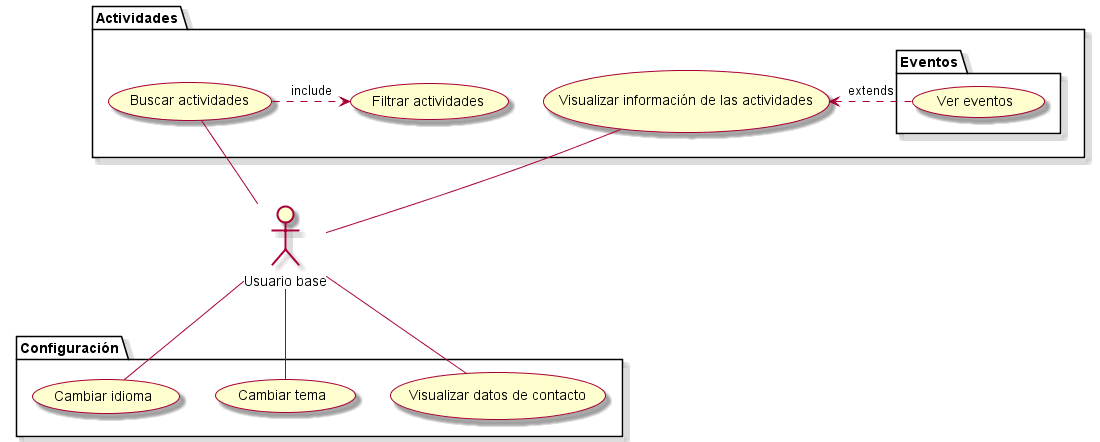
\includegraphics[width=1\linewidth]{5-AnalisisDelSistemaDeInformacion/Casos de uso/usuarioBase/diagrama.png}
	\caption{Diagrama - Usuario base}
\end{figure}
\begin{identificacionCasoDeUso}
	\begin{tabular} { | p{17cm} | }
		\hline
		Nombre del caso de uso                                                                                               \\ \hline
		Buscar actividades                                                                                                   \\ \hline
		Descripción del caso de uso                                                                                          \\ \hline
		Este caso de uso permite a cualquier usuario buscar actividades en el sistema aplicando ciertos filtros de búsqueda. \\ \hline
	\end{tabular}
	\caption{Caso de uso - Buscar actividades}
\end{identificacionCasoDeUso}
\begin{identificacionCasoDeUso}
	\begin{tabular} { | p{17cm} |}

		\hline
		Nombre del caso de uso                                                                                                         \\ \hline
		Visualizar información de las actividades                                                                                      \\ \hline
		Descripción del caso de uso                                                                                                    \\ \hline
		Este caso de uso permite a cualquier usuario ver información detallada sobre una actividad en particular, así como sus eventos \\ \hline
	\end{tabular}
	\caption{Caso de uso - Visualizar información de las actividades}
\end{identificacionCasoDeUso}
\begin{identificacionCasoDeUso}
	\begin{tabular} { | p{17cm} |}

		\hline
		Nombre del caso de uso                                                                                           \\ \hline
		Cambiar idioma                                                                                                   \\ \hline
		Descripción del caso de uso                                                                                      \\ \hline
		Este caso de uso permite a cualquier usuario cambiar el idioma de la aplicación entre inglés, español y francés. \\ \hline
	\end{tabular}
	\caption{Caso de uso - Cambiar idioma}
\end{identificacionCasoDeUso}
\begin{identificacionCasoDeUso}
	\begin{tabular} { | p{17cm} |}
		\hline
		Nombre del caso de uso                                                                                              \\ \hline
		Cambiar tema                                                                                                        \\ \hline
		Descripción del caso de uso                                                                                         \\ \hline
		Este caso de uso permite a cualquier usuario cambiar el tema de la aplicación entre el tema oscuro y el tema claro. \\ \hline
	\end{tabular}
	\caption{Caso de uso - Cambiar tema}
\end{identificacionCasoDeUso}
\begin{identificacionCasoDeUso}
	\begin{tabular} { | p{17cm} |}
		\hline
		Nombre del caso de uso                                                         \\ \hline
		Visualizar datos de contacto                                                   \\ \hline
		Descripción del caso de uso                                                    \\ \hline
		Este caso de uso permite a cualquier usuario visualizar los datos de contacto. \\ \hline
	\end{tabular}
	\caption{Caso de uso - Visualizar datos de contacto}
\end{identificacionCasoDeUso}
\subsubsection{Usuario no identificado}
\begin{figure}[H]
	\centering
	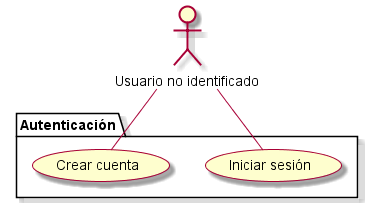
\includegraphics{5-AnalisisDelSistemaDeInformacion//Casos de uso//usuarioNoIdentificado//diagrama.png}
	\caption{Diagrama - Usuario no identificado}
\end{figure}
\begin{identificacionCasoDeUso}
	\begin{tabular} { | p{17cm} |}

		\hline
		Nombre del caso de uso               \\ \hline
		Crear cuenta                         \\ \hline
		Descripción del caso de uso          \\ \hline
		Este caso de uso permite a los usuarios no registrados, crearse una cuenta el sistema proporcionando la siguiente información:
		\begin{itemize}
			\item Nombre y apellidos del usuario
			\item Dirección de correo electronico
			\item Contraseña
			\item País (Opcional)
			\item Fecha de nacimiento (Opcional)
		\end{itemize} \\ \hline
	\end{tabular}
	\caption{Caso de uso - Crear cuenta}
\end{identificacionCasoDeUso}
\begin{identificacionCasoDeUso}
	\begin{tabular} { | p{17cm} |}

		\hline
		Nombre del caso de uso                                                                                                                  \\ \hline
		Iniciar sesión                                                                                                                          \\ \hline
		Descripción del caso de uso                                                                                                             \\ \hline
		Este caso de uso permite a los usuarios no registrados, iniciar sesión en el sistema proporcionando su correo electrónico y contraseña. \\ \hline
	\end{tabular}
	\caption{Caso de uso - Iniciar sesión}
\end{identificacionCasoDeUso}
\subsubsection{Usuario registrado}
\begin{figure}[H]
	\centering
	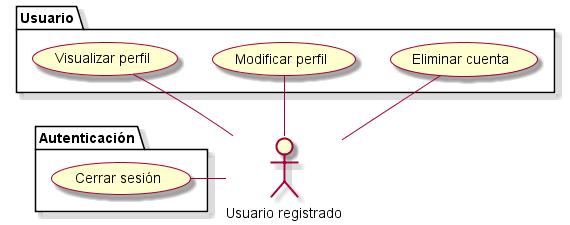
\includegraphics[width=1\linewidth]{5-AnalisisDelSistemaDeInformacion//Casos de uso//usuarioRegistrado/diagrama.png}
	\caption{Diagrama - Usuario registrado}
\end{figure}
\input{5-AnalisisDelSistemaDeInformacion/Casos de uso/usuarioRegistrado/Tablas/tablaCerrarSesión}
\begin{identificacionCasoDeUso}
	\begin{tabular} { | p{17cm} | }
		\hline
		Nombre del caso de uso                                                        \\ \hline
		Visualizar perfil                                                             \\ \hline
		Descripción del caso de uso                                                   \\ \hline
		Este caso de uso permite a los usuarios registrados, ver sus datos personales \\ \hline
	\end{tabular}
	\caption{Caso de uso - Visualizar perfil}
\end{identificacionCasoDeUso}
\begin{identificacionCasoDeUso}
	\begin{tabular} { | p{17cm} |}

		\hline
		Nombre del caso de uso                                                                                     \\ \hline
		Modificar perfil                                                                                           \\ \hline
		Descripción del caso de uso                                                                                \\ \hline
		Este caso de uso permite a los usuarios registrados, modificar su perfil actualizando sus datos personales \\ \hline
	\end{tabular}
	\caption{Caso de uso - Modificar perfil}
\end{identificacionCasoDeUso}
\begin{identificacionCasoDeUso}
	\begin{tabular} { | p{17cm} |}

		\hline
		Nombre del caso de uso                                                  \\ \hline
		Eliminar cuenta                                                         \\ \hline
		Descripción del caso de uso                                             \\ \hline
		Este caso de uso permite a los usuarios registrados, eliminar su cuenta \\ \hline
	\end{tabular}
	\caption{Caso de uso - Eliminar cuenta}
\end{identificacionCasoDeUso}
\subsubsection{Usuario registrado con rol de administrador}
\begin{figure}[H]
	\centering
	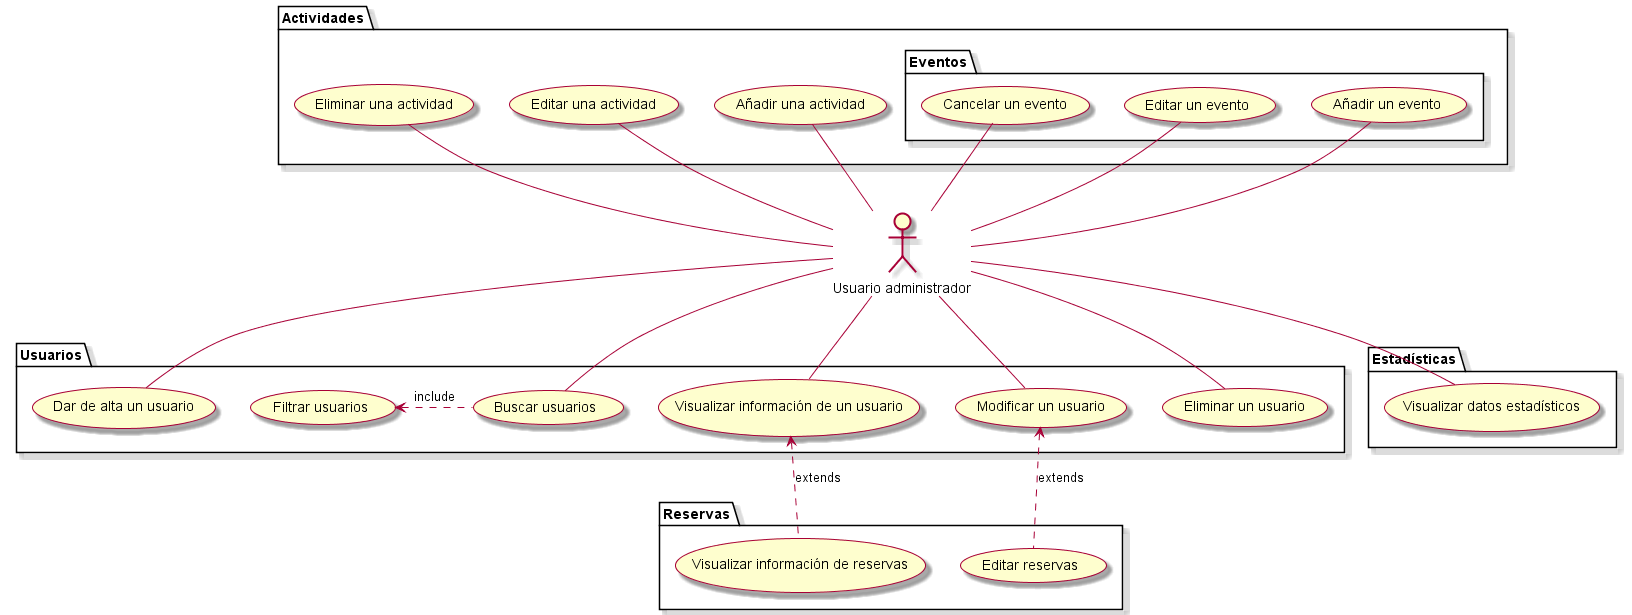
\includegraphics[width=1\linewidth]{5-AnalisisDelSistemaDeInformacion//Casos de uso//usuarioAdministrador/diagrama.png}
	\caption{Diagrama - Usuario administrador}
\end{figure}
\input{5-AnalisisDelSistemaDeInformacion/Casos de uso/usuarioAdministrador/Tablas/tablaAñadirActividad}
\begin{identificacionCasoDeUso}
	\begin{tabular} { | p{17cm} |}

		\hline
		Nombre del caso de uso                                                                                                                              \\ \hline
		Editar una actividad                                                                                                                                \\ \hline
		Descripción del caso de uso                                                                                                                         \\ \hline
		Este caso de uso permite a los usuarios registrados con el rol de administrador, editar la información de una actividad ya existente en el sistema. \\ \hline
	\end{tabular}
	\caption{Caso de uso - Editar una actividad}
\end{identificacionCasoDeUso}
\begin{identificacionCasoDeUso}
	\begin{tabular} { | p{17cm} |}

		\hline
		Nombre del caso de uso                                                                                                            \\ \hline
		Eliminar una actividad                                                                                                            \\ \hline
		Descripción del caso de uso                                                                                                       \\ \hline
		Este caso de uso permite a los usuarios registrados con el rol de administrador, eliminar una actividad ya existente del sistema. \\ \hline
	\end{tabular}
	\caption{Caso de uso - Eliminar una actividad}
\end{identificacionCasoDeUso}
\begin{identificacionCasoDeUso}
	\begin{tabular} { | p{17cm} |}

		\hline
		Nombre del caso de uso                  \\ \hline
		Dar de alta un usuario                  \\ \hline
		Descripción del caso de uso             \\ \hline
		Este caso de uso permite a los usuarios registrados con el rol de administrador, crear una nueva cuenta en el sistema proporcionando la siguiente información:
		\begin{itemize}
			\item Nombre y apellidos del usuario
			\item Dirección de correo electronico
			\item Role que tendrá dentro del sistema
			\item Contraseña
			\item Fecha de nacimiento (Opcional)
			\item Pais (Opcional)
		\end{itemize} \\ \hline
	\end{tabular}
	\caption{Caso de uso - Dar de alta un usuario}
\end{identificacionCasoDeUso}
\begin{identificacionCasoDeUso}
	\begin{tabular} { | p{17cm} |}

		\hline
		Nombre del caso de uso                                                                                                                                                  \\ \hline
		Buscar usuarios                                                                                                                                                         \\ \hline
		Descripción del caso de uso                                                                                                                                             \\ \hline
		Este caso de uso permite a los usuarios registrados con el rol de administrador, realizar búsquedas de usuarios en el sistema utilizando ciertos criterios de búsqueda. \\ \hline
	\end{tabular}
	\caption{Caso de uso - Buscar usuarios}
\end{identificacionCasoDeUso}
\input{5-AnalisisDelSistemaDeInformacion/Casos de uso/usuarioAdministrador/Tablas/tablaVisualizarInformaciónDeUsuario}
\begin{identificacionCasoDeUso}
	\begin{tabular} { | p{17cm} |}

		\hline
		Nombre del caso de uso                                                                                                                           \\ \hline
		Modificar un usuario                                                                                                                             \\ \hline
		Descripción del caso de uso                                                                                                                      \\ \hline
		Este caso de uso permite a los usuarios registrados con el rol de administrador, editar la información de un usuario ya existente en el sistema. \\ \hline
	\end{tabular}
	\caption{Caso de uso - Modificar un usuario}
\end{identificacionCasoDeUso}
\begin{identificacionCasoDeUso}
	\begin{tabular} { | p{17cm} |}

		\hline
		Nombre del caso de uso                                                                                                         \\ \hline
		Eliminar un usuario                                                                                                            \\ \hline
		Descripción del caso de uso                                                                                                    \\ \hline
		Este caso de uso permite a los usuarios registrados con el rol de administrador, eliminar un usuario ya existente del sistema. \\ \hline
	\end{tabular}
	\caption{Caso de uso - Eliminar un usuario}
\end{identificacionCasoDeUso}
\begin{identificacionCasoDeUso}
	\begin{tabular} { | p{17cm} |}
		\hline
		Nombre del caso de uso                       \\ \hline
		Añadir un evento                             \\ \hline
		Descripción del caso de uso                  \\ \hline
		Este caso de uso permite a los usuarios registrados con el rol de administrador, crear un evento de una actividad ya existente en el sistema. Se deberá proporcionar la siguiente información:
		\begin{itemize}
			\item Número de plazas totales a publicar
			\item Idioma en el que se impartirá el evento
			\item Guía asignado
			\item Día y hora del comienzo del evento
		\end{itemize} \\ \hline
	\end{tabular}
	\caption{Caso de uso - Añadir un evento}
\end{identificacionCasoDeUso}
\begin{identificacionCasoDeUso}
	\begin{tabular} { | p{17cm} |}

		\hline
		Nombre del caso de uso                                                                                                                          \\ \hline
		Editar un evento                                                                                                                                \\ \hline
		Descripción del caso de uso                                                                                                                     \\ \hline
		Este caso de uso permite a los usuarios registrados con el rol de administrador, editar la información de un evento ya existente en el sistema. \\ \hline
	\end{tabular}
	\caption{Caso de uso - Editar un evento}
\end{identificacionCasoDeUso}
\begin{identificacionCasoDeUso}
	\begin{tabular} { | p{17cm} |}

		\hline
		Nombre del caso de uso                                                                                                                                  \\ \hline
		Cancelar un evento                                                                                                                                      \\ \hline
		Descripción del caso de uso                                                                                                                             \\ \hline
		Este caso de uso permite a los usuarios registrados con el rol de administrador, cancelar un evento ya existente y que no esté cancelado en el sistema. \\ \hline
	\end{tabular}
	\caption{Caso de uso - Cancelar un evento}
\end{identificacionCasoDeUso}
\begin{identificacionCasoDeUso}
	\begin{tabular} { | p{17cm} |}

		\hline
		Nombre del caso de uso                                                                                                                     \\ \hline
		Visualizar datos estadísticos                                                                                                              \\ \hline
		Descripción del caso de uso                                                                                                                \\ \hline
		Este caso de uso permite a los usuarios registrados con el rol de administrador, visualizar datos estadísticos de las reservas y usuarios. \\ \hline
	\end{tabular}
	\caption{Caso de uso - Visualizar datos estadísticos}
\end{identificacionCasoDeUso}
\subsubsection{Usuario registrado con rol de guía}
\begin{figure}[H]
	\centering
	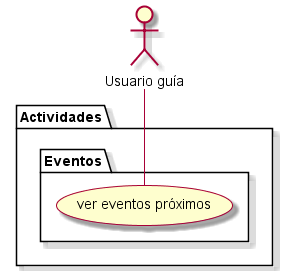
\includegraphics{5-AnalisisDelSistemaDeInformacion//Casos de uso//usuarioGuia/diagrama.png}
	\caption{Diagrama - Usuario guía}
\end{figure}
\begin{identificacionCasoDeUso}
	\begin{tabular} { | p{17cm} |}

		\hline
		Nombre del caso de uso                                                                                                            \\ \hline
		Ver eventos próximos                                                                                                              \\ \hline
		Descripción del caso de uso                                                                                                       \\ \hline
		Este caso de uso permite a los usuarios registrados con rol de guía, obtener un listado de todos los eventos que tiene asignados. \\ \hline
	\end{tabular}
	\caption{Caso de uso - Ver eventos próximos}
\end{identificacionCasoDeUso}
\subsubsection{Usuario registrado con rol de turista}
\begin{figure}[H]
	\centering
	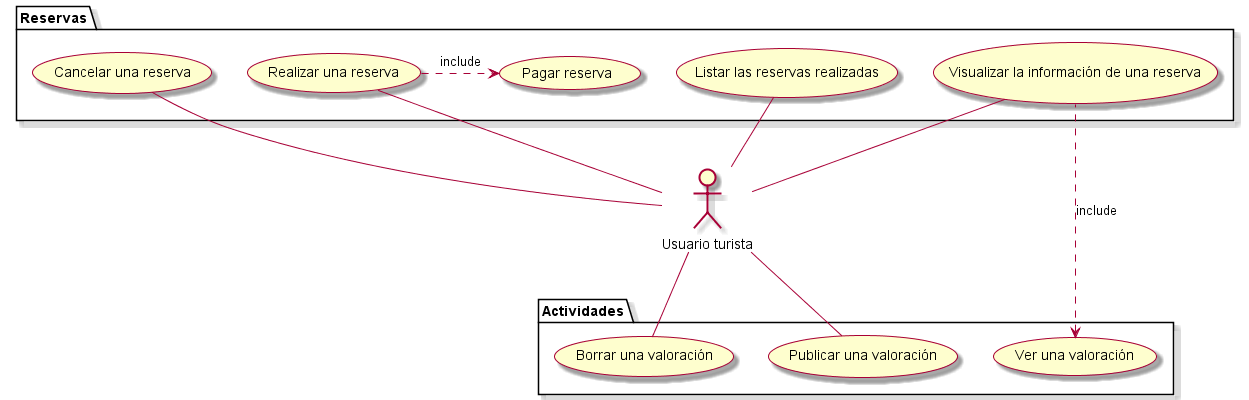
\includegraphics[width=1\linewidth]{5-AnalisisDelSistemaDeInformacion//Casos de uso//usuarioTurista/diagrama.png}
	\caption{Diagrama - Usuario turista}
\end{figure}
\begin{identificacionCasoDeUso}
	\begin{tabular} { | p{17cm} |}

		\hline
		Nombre del caso de uso                                                                                            \\ \hline
		Realizar una reserva                                                                                              \\ \hline
		Descripción del caso de uso                                                                                       \\ \hline
		Este caso de uso permite a los usuarios registrados con el rol de turista, realizar una reserva de una actividad. \\ \hline
	\end{tabular}
	\caption{Caso de uso - Realizar una reserva}
\end{identificacionCasoDeUso}
\begin{identificacionCasoDeUso}
	\begin{tabular} { | p{17cm} |}

		\hline
		Nombre del caso de uso                                                                                                                                \\ \hline
		Cancelar una reserva                                                                                                                                  \\ \hline
		Descripción del caso de uso                                                                                                                           \\ \hline
		Este caso de uso permite a los usuarios registrados con el rol turista, cancelar una reserva ya confirmada, 24 horas antes del inicio de la actividad \\ \hline
	\end{tabular}
	\caption{Caso de uso - Cancelar una reserva}
\end{identificacionCasoDeUso}
\input{5-AnalisisDelSistemaDeInformacion/Casos de uso/usuarioTurista/Tablas/tablaPublicarValoración}
\begin{identificacionCasoDeUso}
	\begin{tabular} { | p{17cm} |}

		\hline
		Nombre del caso de uso                                                                                            \\ \hline
		Borrar una valoración                                                                                             \\ \hline
		Descripción del caso de uso                                                                                       \\ \hline
		Este caso de uso permite a los usuarios registrados con el rol turista, eliminar la valoración que haya publicado \\ \hline
	\end{tabular}
	\caption{Caso de uso - Borrar una valoración}
\end{identificacionCasoDeUso}
\begin{identificacionCasoDeUso}
	\begin{tabular} { | p{17cm} |}

		\hline
		Nombre del caso de uso                                                                                                               \\ \hline
		Listar las reservas realizadas                                                                                                       \\ \hline
		Descripción del caso de uso                                                                                                          \\ \hline
		Este caso de uso permite a los usuarios registrados con el rol de turista, listar todas las reservas realizadas a modo de historial. \\ \hline
	\end{tabular}
	\caption{Caso de uso - Listar las reservas realizadas}
\end{identificacionCasoDeUso}
\input{5-AnalisisDelSistemaDeInformacion/Casos de uso/usuarioTurista/Tablas/tablaVerInformaciónDeLaReserva}

\section{Identificación de Subsistemas}
\subsection{Descripción de los subsistemas}
\subsubsection{Subsistema de gestión de usuarios}
Este subsistema se encarga de todas las operaciones relacionadas con los usuarios de la aplicación. Permite al administrador realizar funciones como la creación, edición, eliminación y listado de usuarios. Además, cualquier usuario puede registrarse, iniciar y cerrar sesión, así como editar su propio perfil.
\subsubsection{Subsistema de gestión de actividades}
Responsable de las operaciones vinculadas a las actividades, este subsistema permite al administrador crear, editar, listar y eliminar actividades. Los usuarios pueden acceder a la información relacionada con cada actividad, incluyendo valoraciones y eventos.
\subsubsection{Subsistema de gestión de reservas}
Este subsistema maneja todas las operaciones relacionadas con las reservas. Los usuarios registrados pueden crear, modificar, cancelar y listar sus reservas. El administrador tiene la capacidad de listar y editar las reservas realizadas por los usuarios.
\subsection*{Descripción de los interfaces entre subsistemas}
\begin{figure}[H]
	\centering
	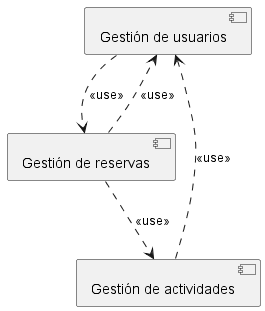
\includegraphics[width=0.5\linewidth]{5-AnalisisDelSistemaDeInformacion/diagrama.png}
	\caption{Diagrama de las relaciones entre los subsistemas}
	\label{fig:diagrama}
\end{figure}
El subsistema de gestión de usuarios interactúa con el subsistema de reservas para obtener las reservas asociadas a un usuario. A su vez, el subsistema de reservas se comunica con el subsistema de usuarios para crear una reserva vinculada a un usuario específico. Este proceso también implica al subsistema de actividades, que recibe información del subsistema de reservas para asociar la actividad que el usuario desea reservar. Finalmente, el subsistema de actividades llama al subsistema de usuarios para asignar un guía a las actividades programadas.
\section{Análisis de los casos de uso}
\subsection{Buscar actividades}
El caso de uso “Buscar actividades” describe cómo los usuarios interactúan con la aplicación para buscar actividades basadas en diferentes criterios.
\begin{analisisCasoDeUso}
	\centering
	\begin{tabular} { | m{3cm} | p{13cm} | }
		\hline
		\multicolumn{2}{ | c | }{\bfseries Buscar actividades}                                                                                                                         \\ \hline
		{\bfseries Precondiciones}  & No.                                                                                                                                              \\ \hline
		{\bfseries Postcondiciones} & Se muestra una lista de actividades que coinciden con los criterios de búsqueda.                                                                 \\ \hline
		{\bfseries Actores    }     & Iniciado por cualquier usuario ya esté identificado o no.                                                                                        \\ \hline
		{\bfseries Descripción}     & {\bfseries 1.} El usuario accede al apartado de búsqueda de actividades en la aplicación.                                                        \\
		                            & {\bfseries 2.} El usuario introduce texto en la barra de búsqueda para filtrar actividades por nombre y ubicación.                               \\
		                            & {\bfseries 3.} El sistema espera a que se deje de escribir para hacer la búsqueda.                                                               \\
		                            & {\bfseries 4.} El sistema muestra una lista de actividades que coinciden con los criterios de búsqueda aplicados.                                \\
		                            & {\bfseries 5.} El usuario puede desplazarse por la lista para ver las actividades que cumplen con los criterios de búsqueda especificados.       \\ \hline
		{\bfseries Variaciones}     & {\bfseries Escenario Alternativo 1:} El usuario realiza una búsqueda sin especificar ningún criterio.                                            \\
		                            & {\bfseries 1.} El usuario accede al apartado de búsqueda de actividades en la aplicación.                                                        \\
		                            & {\bfseries 2.} El sistema muestra la lista de actividades más populares.                                                                         \\
		                            & {\bfseries 3.} Volver al paso 5.                                                                                                                 \\
		                            & {\bfseries Escenario Alternativo 2:} El usuario realiza una búsqueda utilizando los filtros para refinar la búsqueda según fechas, precios, etc. \\
		                            & {\bfseries 1.} El usuario accede al apartado de búsqueda de actividades en la aplicación.                                                        \\
		                            & {\bfseries 2.} El usuario añade filtros de fechas, precios, etc.                                                                                 \\
		                            & {\bfseries 3.} Volver al paso 4.                                                                                                                 \\
		                            & {\bfseries Escenario Alternativo 3:} El sistema no encuentra ninguna actividad que coincida con los criterios de búsqueda.                       \\
		                            & {\bfseries 4.} El sistema muestra un mensaje pidiendo al usuario que cambie los criterios de búsqueda                                            \\ \hline
		{\bfseries Excepciones}     & Si ocurre un error al acceder a la base de datos, se muestra un mensaje de error.                                                                \\ \hline
		{\bfseries Notas }          &                                                                                                                                                  \\ \hline
	\end{tabular}
	\caption{Caso de uso - Buscar actividades}
\end{analisisCasoDeUso}

\subsection{Visualizar información de las actividades}
El caso de uso “Visualizar información de las actividades” describe cómo los usuarios pueden acceder a detalles específicos sobre una actividad seleccionada.
\begin{analisisCasoDeUso}
	\centering
	\begin{tabular} { | m{3cm} | p{13cm} | }
		\hline
		\multicolumn{2}{ | c | }{\bfseries Visualizar información de actividades}                                                                                                         \\ \hline
		{\bfseries Precondiciones}  & No.                                                                                                                                                 \\ \hline
		{\bfseries Postcondiciones} & Se muestra la información detallada de una actividad específica.                                                                                    \\ \hline
		{\bfseries Actores    }     & Iniciado por cualquier usuario ya esté identificado o no.                                                                                           \\ \hline
		{\bfseries Descripción}     & {\bfseries 1.} El usuario selecciona una actividad de la lista de resultados o desde otra parte de la aplicación.                                   \\
		                            & {\bfseries 2.} El sistema muestra la información detallada de la actividad seleccionada, incluyendo descripción, imágenes, ubicación, precios, etc. \\
		                            & {\bfseries 3.} El usuario puede explorar la información.                                                                                            \\ \hline
		{\bfseries Variaciones}     & {\bfseries Escenario alternativo 1:} Actividad eliminada o no disponible.                                                                           \\
		                            & {\bfseries 2.} El sistema muestra un mensaje de error.                                                                                              \\ \hline
		{\bfseries Excepciones}     & Si ocurre un error al acceder a la base de datos, se muestra un mensaje de error.                                                                   \\ \hline
		{\bfseries Notas }          &                                                                                                                                                     \\ \hline
	\end{tabular}
	\caption{Caso de uso - Visualizar información de actividades}
\end{analisisCasoDeUso}
\subsection{Cambiar idioma}
El caso de uso “Cambiar idioma” permite a los usuarios seleccionar el idioma en el que prefieren visualizar la aplicación.
\begin{analisisCasoDeUso}
	\centering
	\begin{tabular} { | m{3cm} | p{13cm} | }
		\hline
		\multicolumn{2}{ | c | }{\bfseries Cambiar idioma}                                                                               \\ \hline
		{\bfseries Precondiciones}  & En caso de estar en la aplicación web, tener las cookies habilitadas en el navegador.              \\ \hline
		{\bfseries Postcondiciones} & Se muestra la aplicación en el idioma seleccionado.                                                \\ \hline
		{\bfseries Actores    }     & Iniciado por cualquier usuario ya esté identificado o no.                                          \\ \hline
		{\bfseries Descripción}     & {\bfseries 1.} El usuario selecciona en el menú la opción para cambiar el idioma de la aplicación. \\
		                            & {\bfseries 2.} El sistema muestra una lista de idiomas disponibles.                                \\
		                            & {\bfseries 3.} El usuario selecciona el idioma deseado.                                            \\
		                            & {\bfseries 4.} El sistema actualiza el idioma de la aplicación según la selección del usuario.     \\
		                            & {\bfseries 5.} El usuario puede ver la aplicación con el idioma cambiado.                          \\ \hline
		{\bfseries Variaciones}     & No.                                                                                                \\ \hline
		{\bfseries Excepciones}     & Si ocurre un error en el proceso de cambio de idioma, se muestra un mensaje de error.              \\ \hline
		{\bfseries Notas }          &                                                                                                    \\ \hline
	\end{tabular}
	\caption{Caso de uso - Cambiar idioma}
\end{analisisCasoDeUso}

\subsection{Cambiar tema}
El caso de uso “Cambiar tema” permite a los usuarios cambiar la apariencia de la aplicación seleccionando diferentes temas.
\begin{analisisCasoDeUso}
	\centering
	\begin{tabular} { | m{3cm} | p{13cm} | }
		\hline
		\multicolumn{2}{ | c | }{\bfseries Cambiar tema}                                                                                         \\ \hline
		{\bfseries Precondiciones}  & En caso de estar en la aplicación web, tener las cookies habilitadas en el navegador.                      \\ \hline
		{\bfseries Postcondiciones} & Se muestra la aplicación en el tema seleccionado.                                                          \\ \hline
		{\bfseries Actores    }     & Iniciado por cualquier usuario ya esté identificado o no.                                                  \\ \hline
		{\bfseries Descripción}     & {\bfseries 1.} El usuario selecciona en el menú la opción para cambiar el tema de la aplicación.           \\
		                            & {\bfseries 2.} El sistema cambia el tema de la aplicación según el tema que estaba aplicado anteriormente. \\
		                            & {\bfseries 3.} El usuario puede ver la aplicación con el tema cambiado.                                    \\ \hline
		{\bfseries Variaciones}     & No.                                                                                                        \\ \hline
		{\bfseries Excepciones}     & Si ocurre un error en el proceso de cambio de tema, se muestra un mensaje de error.                        \\ \hline
		{\bfseries Notas }          &                                                                                                            \\ \hline
	\end{tabular}
	\caption{Caso de uso - Cambiar tema}
\end{analisisCasoDeUso}

\subsection{Visualizar datos de contacto}
El caso de uso “Visualizar datos de contacto” permite a los usuarios acceder a la información de contacto almacenada en el sistema.
\begin{analisisCasoDeUso}
	\centering
	\begin{tabular} { | m{3cm} | p{13cm} | }
		\hline
		\multicolumn{2}{ | c | }{\bfseries Visualizar datos de contacto}                                                \\ \hline
		{\bfseries Precondiciones}  & No.                                                                               \\ \hline
		{\bfseries Postcondiciones} & El usuario desea visualizar los datos de contacto.                                \\ \hline
		{\bfseries Actores    }     & Iniciado por cualquier usuario ya esté identificado o no.                         \\ \hline
		{\bfseries Descripción}     & 1. El usuario accede a cualquier página del sistema.                              \\
		                            & 2. El sistema muestra los datos de contacto en el pie de la página.               \\ \hline
		{\bfseries Variaciones}     & No.                                                                                \\ \hline
		{\bfseries Excepciones}     & Si ocurre un error al acceder a la base de datos, se muestra un mensaje de error. \\ \hline
		{\bfseries Notas }          &                                                                                   \\ \hline
	\end{tabular}
	\caption{Caso de uso - Visualizar datos de contacto}
\end{analisisCasoDeUso}


\subsection{Crear cuenta}
El caso de uso “Crear cuenta” describe el proceso mediante el cual un nuevo usuario puede registrarse en el sistema
\begin{analisisCasoDeUso}
	\centering
	\begin{tabular} { | m{3cm} | p{13cm} | }
		\hline
		\multicolumn{2}{ | c | }{\bfseries Crear cuenta}                                                                        \\ \hline
		{\bfseries Precondiciones}  & No.                                                                                       \\ \hline
		{\bfseries Postcondiciones} & El usuario queda registrado en el sistema e inicia sesión automáticamente.                \\ \hline
		{\bfseries Actores    }     & Iniciado por cualquier usuario sin identificar                                            \\ \hline
		{\bfseries Descripción}     & {\bfseries 1.} El usuario selecciona en el menú la opción “Cuenta” .                       \\
		                            & {\bfseries 2.} El sistema muestra la página de inicio de sesión.                          \\
		                            & {\bfseries 3.} El usuario selecciona la opción “Regístrate aquí” .                         \\
		                            & {\bfseries 4.} El sistema muestra la página de registro.                                  \\
		                            & {\bfseries 5.} El usuario introduce los datos requeridos.                                 \\
		                            & {\bfseries 6.} El usuario envía el formulario de registro.                                \\
		                            & {\bfseries 7.} El sistema valida los datos del formulario.                                \\
		                            & {\bfseries 8.} El sistema registra los datos del usuario en la base de datos.             \\
		                            & {\bfseries 9.} El sistema confirma el registro del usuario.                               \\ \hline
		{\bfseries Variaciones}     & {\bfseries Escenario alternativo 1:} En caso de que los datos ingresados no sean válidos. \\
		                            & {\bfseries 8.} El sistema muestra un mensaje de error.                                    \\
		                            & {\bfseries Volver al paso 4.}                                                             \\ \hline
		{\bfseries Excepciones}     & Si ocurre un error en el proceso de registro, se muestra un mensaje de error.             \\ \hline
		{\bfseries Notas }          &                                                                                           \\ \hline
	\end{tabular}
	\caption{Caso de uso - Crear cuenta}
\end{analisisCasoDeUso}
\subsection{Iniciar sesión}
El caso de uso “Iniciar sesión” permite a los usuarios registrados acceder a sus cuentas en el sistema.
\begin{analisisCasoDeUso}
	\centering
	\begin{tabular} { | m{3cm} | p{13cm} | }
		\hline
		\multicolumn{2}{ | c | }{\bfseries Iniciar sesión}                                                                       \\ \hline
		{\bfseries Precondiciones}  & El usuario debe haberse creado una cuenta en el sistema.                                   \\ \hline
		{\bfseries Postcondiciones} & El usuario queda identificado.                                                             \\ \hline
		{\bfseries Actores    }     & Iniciado por cualquier usuario sin identificar                                             \\ \hline
		{\bfseries Descripción}     & {\bfseries 1.} El usuario selecciona en el menú la opción “Área Personal” .                 \\
		                            & {\bfseries 2.} El sistema muestra la página de inicio de sesión.                           \\
		                            & {\bfseries 3.} El usuario introduce los datos requeridos.                                  \\
		                            & {\bfseries 4.} El usuario envía el formulario de registro.                                 \\
		                            & {\bfseries 5.} El sistema verifica los datos del formulario.                               \\
		                            & {\bfseries 6.} El usuario queda identificado.                                              \\ \hline
		{\bfseries Variaciones}     & {\bfseries Escenario alternativo 1:} En caso de que los datos ingresados sean incorrectos. \\
		                            & {\bfseries 6.} El sistema muestra un mensaje de error.                                     \\ \hline
		{\bfseries Excepciones}     & Si ocurre un error en el proceso de inicio de sesión, se muestra un mensaje de error.      \\
		{\bfseries Notas }          &                                                                                            \\ \hline
	\end{tabular}
	\caption{Caso de uso - Iniciar sesión}
\end{analisisCasoDeUso}
\subsection{Cerrar sesión}
El caso de uso “Cerrar sesión” describe el proceso mediante el cual un usuario puede salir de su cuenta en el sistema de manera segura.
\begin{analisisCasoDeUso}
	\centering
	\begin{tabular} { | m{3cm} | p{13cm} | }
		\hline
		\multicolumn{2}{ | c | }{\bfseries Cerrar sesión}                                                                   \\ \hline
		{\bfseries Precondiciones}  & No.                                                                                   \\ \hline
		{\bfseries Postcondiciones} & El usuario cierra sesión en el sistema.                                               \\ \hline
		{\bfseries Actores    }     & Iniciado por cualquier usuario identificado.                                          \\ \hline
		{\bfseries Descripción}     & {\bfseries 1.} El usuario selecciona en el menú la opción “Área Personal” .            \\
		                            & {\bfseries 2.} El sistema muestra la página de perfil.                                \\
		                            & {\bfseries 3.} El usuario visualiza la información de su perfil.                      \\
		                            & {\bfseries 4.} El usuario selecciona la opción “Cerrar sesión” .                       \\
		                            & {\bfseries 5.} El sistema cierra la sesión del usuario.                               \\ \hline
		{\bfseries Variaciones}     & No.                                                                                   \\ \hline
		{\bfseries Excepciones}     & Si ocurre un error en el proceso de cierre de sesión, se muestra un mensaje de error. \\ \hline
		{\bfseries Notas }          &                                                                                       \\ \hline
	\end{tabular}
	\caption{Caso de uso - Cerrar sesión}
\end{analisisCasoDeUso}
\subsection{Visualizar perfil}
El caso de uso “Visualizar perfil” permite a los usuarios acceder y ver la información de su perfil personal.
\begin{analisisCasoDeUso}
	\centering
	\begin{tabular} { | m{3cm} | p{13cm} | }
		\hline
		\multicolumn{2}{ | c | }{\bfseries Visualizar perfil}                                                    \\ \hline
		{\bfseries Precondiciones}  & No.                                                                        \\ \hline
		{\bfseries Postcondiciones} & Se muestra la información del perfil del usuario.                          \\ \hline
		{\bfseries Actores    }     & Iniciado por cualquier usuario identificado.                               \\ \hline
		{\bfseries Descripción}     & {\bfseries 1.} El usuario selecciona en el menú la opción “Área Personal” . \\
		                            & {\bfseries 2.} El sistema muestra la página de perfil.                     \\
		                            & {\bfseries 3.} El usuario visualiza la información de su perfil.           \\ \hline
		{\bfseries Variaciones}     & No.                                                                        \\ \hline
		{\bfseries Excepciones}     & Si ocurre un error en la base de datos, se muestra un mensaje de error.    \\ \hline
		{\bfseries Notas }          &                                                                            \\ \hline
	\end{tabular}
	\caption{Caso de uso - Visualizar perfil}
\end{analisisCasoDeUso}
\subsection{Modificar perfil}
El caso de uso “Modificar perfil” permite a los usuarios editar y actualizar la información de su perfil personal.
\begin{analisisCasoDeUso}
	\centering
	\begin{tabular} { | m{3cm} | p{13cm} | }
		\hline
		\multicolumn{2}{ | c | }{\bfseries Modificar perfil}                                                                   \\ \hline
		{\bfseries Precondiciones}  & No.                                                                                      \\ \hline
		{\bfseries Postcondiciones} & Los cambios realizados en el perfil del usuario son guardados.                           \\ \hline
		{\bfseries Actores    }     & Iniciado por cualquier usuario identificado.                                             \\ \hline
		{\bfseries Descripción}     & {\bfseries 1.} El usuario selecciona en el menú la opción “Área Personal” .               \\
		                            & {\bfseries 2.} El sistema muestra la página de perfil.                                   \\
		                            & {\bfseries 3.} El usuario visualiza la información de su perfil.                         \\
		                            & {\bfseries 4.} El usuario selecciona la opción “Editar datos de perfil” .                 \\
		                            & {\bfseries 5.} El sistema muestra un formulario con los datos del perfil del usuario.    \\
		                            & {\bfseries 6.} El usuario realiza los cambios deseados en la información del perfil.     \\
		                            & {\bfseries 7.} El usuario guarda los cambios.                                            \\
		                            & {\bfseries 8.} El sistema valida los nuevos datos del perfil.                            \\
		                            & {\bfseries 9.} El sistema actualiza los datos del usuario en el sistema.                 \\ \hline
		{\bfseries Variaciones}     & {\bfseries Escenario alternativo 1:} En caso de que los datos cambiados no sean válidos. \\
		                            & {\bfseries 9.} El sistema muestra un mensaje de error.                                   \\
		                            & {\bfseries 10.} Volver al paso 3.                                                        \\
		                            & {\bfseries Escenario alternativo 2:} En caso de que no se quiera hacer un cambio.        \\
		                            & {\bfseries 7.} El usuario cancela la edición.                                            \\
		                            & {\bfseries 8.} El usuario visualiza la información de su perfil.                         \\ \hline
		{\bfseries Excepciones}     & Si ocurre un error en el proceso de edición del perfil, se muestra un mensaje de error.  \\ \hline
		{\bfseries Notas }          &                                                                                          \\ \hline
	\end{tabular}
	\caption{Caso de uso - Modificar perfil}
\end{analisisCasoDeUso}
\subsection{Eliminar cuenta}
El caso de uso “Eliminar cuenta” describe el proceso mediante el cual un usuario puede eliminar su cuenta del sistema.
\begin{analisisCasoDeUso}
	\centering
	\begin{tabular} { | m{3cm} | p{13cm} | }
		\hline
		\multicolumn{2}{ | c | }{\bfseries Eliminar cuenta}                                                                      \\ \hline
		{\bfseries Precondiciones}  & El usuario debe estar identificado.                                                        \\ \hline
		{\bfseries Postcondiciones} & La cuenta del usuario es eliminada del sistema y se cierra sesión en el sistema.           \\ \hline
		{\bfseries Actores    }     & Usuario                                                                                    \\ \hline
		{\bfseries Descripción}     & {\bfseries 1.} El usuario selecciona en el menú la opción “Área Personal” .                 \\
		                            & {\bfseries 2.} El sistema muestra la página de perfil.                                     \\
		                            & {\bfseries 3.} El usuario visualiza la información de su perfil.                           \\
		                            & {\bfseries 4.} El usuario selecciona la opción “Eliminar Cuenta” .                          \\
		                            & {\bfseries 5.} El sistema pide confirmación.                                               \\
		                            & {\bfseries 6.} El usuario confirma la eliminación                                          \\
		                            & {\bfseries 7.} El sistema elimina la cuenta.                                               \\
		                            & {\bfseries 8.} El sistema cierra la sesión del usuario.                                    \\ \hline
		{\bfseries Variaciones}     & {\bfseries Escenario alternativo 1:} En caso de que se cancele la eliminación              \\
		                            & {\bfseries 6.} El usuario cancela la eliminación                                           \\
		                            & {\bfseries 7.} El sistema cancela la eliminación                                           \\ \hline
		{\bfseries Excepciones}     & Si ocurre un error en el proceso de eliminación de cuenta, se muestra un mensaje de error. \\ \hline
		{\bfseries Notas }          &                                                                                            \\ \hline
	\end{tabular}
	\caption{Caso de uso - Eliminar cuenta}
\end{analisisCasoDeUso}
\subsection{Añadir una actividad}
El caso de uso “Añadir una actividad” permite a los administradores del sistema agregar nuevas actividades al sistema.
\begin{analisisCasoDeUso}
	\centering
	\begin{tabular} { | m{3cm} | p{13cm} | }
		\hline
		\multicolumn{2}{ | c | }{\bfseries Añadir una actividad}                                                                           \\ \hline
		{\bfseries Precondiciones}  & Estar accediendo a la aplicación a través de un ordenador.                                           \\ \hline
		{\bfseries Postcondiciones} & Registrar en el sistema una nueva actividad.                                                         \\ \hline
		{\bfseries Actores    }     & Iniciado por cualquier usuario con rol administrador.                                                \\ \hline
		{\bfseries Descripción}     & {\bfseries 1.} El usuario selecciona en el menú la opción “Dashboard” .                               \\
		                            & {\bfseries 2.} El sistema muestra la pantalla principal del dashboard junto a un menú lateral.       \\
		                            & {\bfseries 3.} El usuario selecciona en el menú lateral la opción “Actividades” .                     \\
		                            & {\bfseries 4.} El sistema muestra un listado de actividades ya existentes.                           \\
		                            & {\bfseries 5.} El usuario selecciona el botón “Añadir actividad” .                                    \\
		                            & {\bfseries 6.} El sistema muestra un formulario.                                                     \\
		                            & {\bfseries 7.} El usuario introduce los datos requeridos.                                            \\
		                            & {\bfseries 8.} El usuario envía el formulario de creación de actividad.                              \\
		                            & {\bfseries 9.} El sistema verifica los datos del formulario.                                         \\
		                            & {\bfseries 10.} El sistema registra los datos de la nueva actividad en la base de datos.             \\\hline
		{\bfseries Variaciones}     & {\bfseries Escenario Alternativo 1} El usuario cancela la creación de la nueva actividad             \\
		                            & {\bfseries 8.} El usuario presiona la opción “Cerrar”.                                               \\
		                            & {\bfseries 9.} El sistema cierra el formulario.                                                      \\
		                            & {\bfseries Escenario Alternativo 2} El usuario no rellena correctamente el formulario.               \\
		                            & {\bfseries 10.} El sistema muestra un mensaje de error                                               \\
		                            & {\bfseries 11.} Volver al paso 7.                                                                    \\ \hline
		{\bfseries Excepciones}     & Si ocurre un error en el proceso de creación de una nueva actividad, se muestra un mensaje de error. \\ \hline
		{\bfseries Notas }          &                                                                                                      \\ \hline
	\end{tabular}
	\caption{Caso de uso - Añadir una actividad}
\end{analisisCasoDeUso}
\subsection{Editar una actividad}
El caso de uso “Editar una actividad” describe cómo los administradores pueden modificar la información de las actividades existentes en el sistema.
\begin{analisisCasoDeUso}
	\centering
	\begin{tabular} { | m{3cm} | p{13cm} | }
		\hline
		\multicolumn{2}{ | c | }{\bfseries Editar una actividad}                                                                     \\ \hline
		{\bfseries Precondiciones}  & Debe haber actividades registradas.                                                            \\ \hline
		{\bfseries Postcondiciones} & La actividad refleja los cambios realizados                                                    \\ \hline
		{\bfseries Actores    }     & Usuario identificado con rol administrador.                                                    \\ \hline
		{\bfseries Descripción}     & {\bfseries 1.} El usuario selecciona en el menú la opción “Dashboard” .                         \\
		                            & {\bfseries 2.} El sistema muestra la pantalla principal del dashboard junto a un menú lateral. \\
		                            & {\bfseries 3.} El usuario selecciona en el menú lateral la opción “Actividades” .               \\
		                            & {\bfseries 4.} El sistema muestra un listado de actividades ya existentes.                     \\
		                            & {\bfseries 5.} El usuario selecciona la opción “Editar” de la actividad que quiere editar.     \\
		                            & {\bfseries 6.} El usuario realiza los cambios deseados.                                        \\
		                            & {\bfseries 7.} El sistema valida los datos.                                                    \\
		                            & {\bfseries 8.} El sistema actualiza la actividad.                                              \\ \hline
		{\bfseries Variaciones}     & {\bfseries Escenario alternativo 1:} Si los datos ingresados son incorrectos.                  \\
		                            & {\bfseries 8.} El sistema muestra un mensaje de error.                                         \\
		                            & {\bfseries 9.} Vuelve al paso 6.                                                               \\ \hline
		{\bfseries Excepciones}     & Si ocurre un error en el proceso de edición, se muestra un mensaje de error.                   \\ \hline
		{\bfseries Notas }          &                                                                                                \\ \hline
	\end{tabular}
	\caption{Caos de uso - Editar una actividad}
\end{analisisCasoDeUso}
\subsection{Eliminar una actividad}
El caso de uso “Eliminar una actividad” permite a los administradores eliminar actividades del sistema.
\begin{analisisCasoDeUso}
	\centering
	\begin{tabular} { | m{3cm} | p{13cm} | }
		\hline
		\multicolumn{2}{ | c | }{\bfseries Eliminar una actividad}                                                                   \\ \hline
		{\bfseries Precondiciones}  & Debe haber actividades registradas.                                                            \\ \hline
		{\bfseries Postcondiciones} & Se eliminan actividades previamente registradas.                                               \\ \hline
		{\bfseries Actores    }     & Usuario identificado con rol administrador.                                      \\ \hline
		{\bfseries Descripción}     & {\bfseries 1.} El usuario selecciona en el menú la opción “Dashboard” .                         \\
		                            & {\bfseries 2.} El sistema muestra la pantalla principal del dashboard junto a un menú lateral. \\
		                            & {\bfseries 3.} El usuario selecciona en el menú lateral la opción “Actividades” .               \\
		                            & {\bfseries 4.} El sistema muestra un listado de actividades ya existentes.                     \\
		                            & {\bfseries 5.} El usuario selecciona la opción “Eliminar” de la actividad que quiere eliminar. \\
		                            & {\bfseries 6.} El sistema pide confirmación.                                                   \\
		                            & {\bfseries 7.} El usuario confirma la eliminación.                                             \\
		                            & {\bfseries 8.} El sistema elimina la actividad.                                                \\ \hline
		{\bfseries Variaciones}     & {\bfseries Escenario Alternativo 1} El usuario cancela la eliminación de la actividad          \\
		                            & {\bfseries 8.} El usuario presiona la opción “Cancelar”.                                       \\
		                            & {\bfseries 9.} El sistema cancela la eliminación.                                              \\ \hline
		{\bfseries Excepciones}     & Si ocurre un error en el proceso de eliminación, se muestra un mensaje de error.               \\ \hline
		{\bfseries Notas }          &                                                                                                \\ \hline
	\end{tabular}
	\caption{Caso de uso - Eliminar una actividad}
\end{analisisCasoDeUso}
\subsection{Dar de alta un usuario}
El caso de uso “Dar de alta un usuario” permite a los administradores registrar nuevos usuarios en el sistema.
\begin{analisisCasoDeUso}
	\centering
	\begin{tabular} { | m{3cm} | p{13cm} | }
		\hline
		\multicolumn{2}{ | c | }{\bfseries Dar de alta un usuario}                                                                   \\ \hline
		{\bfseries Precondiciones}  & No.                                                                                            \\ \hline
		{\bfseries Postcondiciones} & Se registra el nuevo usuario en el sistema                                                     \\ \hline
		{\bfseries Actores    }     & Usuario identificado con rol administrador.                                      \\ \hline
		{\bfseries Descripción}     & {\bfseries 1.} El usuario selecciona en el menú la opción “Dashboard” .                         \\
		                            & {\bfseries 2.} El sistema muestra la pantalla principal del dashboard junto a un menú lateral. \\
		                            & {\bfseries 3.} El usuario selecciona en el menú lateral la opción “Usuarios” .                  \\
		                            & {\bfseries 4.} El sistema muestra un listado de usuarios ya registrados.                       \\
		                            & {\bfseries 5.} El usuario selecciona el botón “Añadir” .                                        \\
		                            & {\bfseries 6.} El sistema muestra un formulario.                                               \\
		                            & {\bfseries 7.} El usuario ingresa los detalles del nuevo usuario.                              \\
		                            & {\bfseries 8.} El usuario presiona el botón de guardar.                                        \\
		                            & {\bfseries 9.} El sistema valida los datos.                                                    \\
		                            & {\bfseries 10.} El sistema registra el nuevo usuario en la base de datos.                      \\ \hline
		{\bfseries Variaciones}     & {\bfseries Escenario alternativo 1} Si los datos ingresados son incorrectos.                   \\
		                            & {\bfseries 10.} El sistema muestra un mensaje de error.                                        \\
		                            & {\bfseries 11.} Vuelve al paso 7.                                                              \\
		                            & {\bfseries Escenario Alternativo 2} El usuario cancela la creación del nuevo usuario.          \\
		                            & {\bfseries 8.} El usuario presiona la opción “Cerrar” .                                         \\
		                            & {\bfseries 9.} El sistema cierra el formulario.                                                \\\hline
		{\bfseries Excepciones}     & Si ocurre un error en el proceso de creación, se muestra un mensaje de error.                  \\ \hline
		{\bfseries Notas }          &                                                                                                \\ \hline
	\end{tabular}
	\caption{Caso de uso - Dar de alta un usuario}
\end{analisisCasoDeUso}
\subsection{Buscar usuarios}
El caso de uso “Buscar usuarios” permite a los administradores encontrar usuarios específicos en el sistema utilizando diferentes criterios de búsqueda.
\begin{analisisCasoDeUso}
	\centering
	\begin{tabular} { | m{3cm} | p{13cm} | }
		\hline
		\multicolumn{2}{ | c | }{\bfseries Buscar usuarios}                                                                                                   \\ \hline
		{\bfseries Precondiciones}  & No.                                                                                                                     \\ \hline
		{\bfseries Postcondiciones} & Se muestra una lista de usuarios que coinciden con los criterios de búsqueda.                                           \\ \hline
		{\bfseries Actores    }     & Usuario identificado con rol administrador.                                                               \\ \hline
		{\bfseries Descripción}     & {\bfseries 1.} El usuario selecciona en el menú la opción “Dashboard” .                                                  \\
		                            & {\bfseries 2.} El sistema muestra la pantalla principal del dashboard junto a un menú lateral.                          \\
		                            & {\bfseries 3.} El usuario selecciona en el menú lateral la opción “Usuarios” .                                           \\
		                            & {\bfseries 4.} El sistema muestra un listado de usuarios.                                                               \\\hline
		{\bfseries Variaciones}     & {\bfseries Escenario alternativo 1:} El usuario realiza una búsqueda filtrando por cadena de texto.                     \\
		                            & {\bfseries 5.} El usuario introduce texto en la barra de búsqueda para filtrar por nombre y correo electrónico.         \\
		                            & {\bfseries 6.} El sistema espera a que se deje de escribir para hacer la búsqueda.                                      \\
		                            & {\bfseries 7.} Volver al paso 4.                                                                                        \\
		                            & que cumplen con los criterios de búsqueda especificados.                                                                \\
		                            & {\bfseries Escenario alternativo 2:} El usuario realiza una búsqueda utilizando los filtros para refinar la búsqueda.   \\
		                            & {\bfseries 5.} El usuario accede al apartado de búsqueda de actividades en la aplicación.                               \\
		                            & {\bfseries 6.} El usuario añade filtros de role, país, etc.                                                             \\
		                            & {\bfseries 7.} El sistema realiza la búsqueda aplicando los filtros.                                                    \\
		                            & {\bfseries 8.} Volver al paso 4.                                                                                        \\
		                            & {\bfseries Escenario alternativo 3:} El sistema no encuentra ningún usuario que coincida con los criterios de búsqueda. \\
		                            & {\bfseries 4.} El sistema muestra un mensaje pidiendo al usuario que cambie los criterios de búsqueda.                  \\ \hline
		{\bfseries Excepciones}     & Si ocurre un error al acceder a la base de datos, se muestra un mensaje de error.                                       \\ \hline
		{\bfseries Notas }          &                                                                                                                         \\ \hline
	\end{tabular}
	\caption{Caso de uso - Buscar usuarios}
\end{analisisCasoDeUso}
\subsection{Visualizar información de un usuario}
l caso de uso “Visualizar información de un usuario” permite a los administradores acceder a los detalles específicos de un usuario registrado.
\begin{analisisCasoDeUso}
	\centering
	\begin{tabular} { | m{3cm} | p{13cm} | }
		\hline
		\multicolumn{2}{ | c | }{\bfseries Visualizar información de un usuario}                                                     \\ \hline
		{\bfseries Precondiciones}  & Debe haber usuarios registrados en el sistema.                                                 \\ \hline
		{\bfseries Postcondiciones} & Se muestra la información detallada de un usuario.                                             \\ \hline
		{\bfseries Actores    }     & Usuario identificado con rol administrador.                                                     \\ \hline
		{\bfseries Descripción}     & {\bfseries 1.} El usuario selecciona en el menú la opción “Dashboard” .                         \\
		                            & {\bfseries 2.} El sistema muestra la pantalla principal del dashboard junto a un menú lateral. \\
		                            & {\bfseries 3.} El usuario selecciona en el menú lateral la opción “Usuarios” .                  \\
		                            & {\bfseries 4.} El sistema muestra una lista de usuarios registrados.                           \\
		                            & {\bfseries 5.} El usuario selecciona un usuario para ver más detalles.                         \\
		                            & {\bfseries 6.} El sistema muestra la información detallada del usuario.                        \\ \hline
		{\bfseries Variaciones}     & No.                                                                                            \\ \hline
		{\bfseries Excepciones}     & Si ocurre un error al acceder a la base de datos, se muestra un mensaje de error.              \\ \hline
		{\bfseries Notas }          &                                                                                                \\ \hline
	\end{tabular}
	\caption{Caso de uso - Visualizar información de un usuario}
\end{analisisCasoDeUso}

\subsection{Modificar un usuario}
El caso de uso “Modificar un usuario” permite a los administradores editar y actualizar la información de los usuarios existentes en el sistema.
\begin{analisisCasoDeUso}
	\centering
	\begin{tabular} { | m{3cm} | p{13cm} | }
		\hline
		\multicolumn{2}{ | c | }{\bfseries Modificar un usuario}                                                                     \\ \hline
		{\bfseries Precondiciones}  & Debe haber usuarios registrados en el sistema.                                                 \\ \hline
		{\bfseries Postcondiciones} & Se muestra la información detallada de un usuario.                                             \\ \hline
		{\bfseries Actores    }     & Usuario identificado con rol administrador.                                                    \\ \hline
		{\bfseries Descripción}     & {\bfseries 1.} El usuario selecciona en el menú la opción “Dashboard” .                         \\
		                            & {\bfseries 2.} El sistema muestra la pantalla principal del dashboard junto a un menú lateral. \\
		                            & {\bfseries 3.} El usuario selecciona en el menú lateral la opción “Usuarios” .                  \\
		                            & {\bfseries 4.} El sistema muestra una lista de usuarios registrados.                           \\
		                            & {\bfseries 5.} El usuario selecciona la opción “Editar” del usuario a modificar.               \\
		                            & {\bfseries 6.} El usuario realiza los cambios deseados en la información del usuario.          \\
		                            & {\bfseries 7.} El sistema valida los datos.                                                    \\
		                            & {\bfseries 8.} El sistema actualiza los datos del usuario.                                     \\ \hline
		{\bfseries Variaciones}     & {\bfseries Escenario alternativo 1:} Si los datos ingresados no tienen el formato correcto.    \\
		                            & {\bfseries 1.} El sistema muestra un mensaje de error.                                         \\
		                            & {\bfseries 2.} Vuelta al paso 6.                                                               \\ \hline
		{\bfseries Excepciones}     & Si ocurre un error en el proceso de edición, se muestra un mensaje de error.                   \\ \hline
		{\bfseries Notas }          &                                                                                                \\ \hline
	\end{tabular}
	\caption{Caso de uso - Modificar un usuario}
\end{analisisCasoDeUso}
\subsection{Eliminar un usuario}
El caso de uso “Eliminar un usuario” permite a los administradores eliminar a un usuario del sistema.
\begin{analisisCasoDeUso}
	\centering
	\begin{tabular} { | m{3cm} | p{13cm} | }
		\hline
		\multicolumn{2}{ | c | }{\bfseries Eliminar un usuario}                                                                      \\ \hline
		{\bfseries Precondiciones}  & Debe existir el usuario en el sistema.                                                         \\ \hline
		{\bfseries Postcondiciones} & Se elimina el usuario del sistema.                                                             \\ \hline
		{\bfseries Actores    }     & Usuario identificado con rol administrador.                                                    \\ \hline
		{\bfseries Descripción}     & {\bfseries 1.} El usuario selecciona en el menú la opción “Dashboard” .                         \\
		                            & {\bfseries 2.} El sistema muestra la pantalla principal del dashboard junto a un menú lateral. \\
		                            & {\bfseries 3.} El usuario selecciona en el menú lateral la opción “Usuarios” .                  \\
		                            & {\bfseries 4.} El sistema muestra un listado de usuarios ya existentes.                        \\
		                            & {\bfseries 5.} El usuario selecciona la opción “Eliminar” del usuario a eliminar.              \\
		                            & {\bfseries 6.} El sistema pide confirmación.                                                   \\
		                            & {\bfseries 7.} El usuario confirma la eliminación.                                             \\
		                            & {\bfseries 8.} El sistema elimina la cuenta del usuario.                                       \\ \hline
		{\bfseries Variaciones}     & No.                                                                                            \\ \hline
		{\bfseries Excepciones}     & Si ocurre un error en el proceso de eliminación, se muestra un mensaje de error.               \\ \hline
		{\bfseries Notas }          &                                                                                                \\ \hline
	\end{tabular}
	\caption{Caso de uso - Eliminar un usuario}
\end{analisisCasoDeUso}
\subsection{Añadir un evento}
El caso de uso “Añadir un evento” permite a los administradores crear nuevos eventos en el sistema.
\begin{analisisCasoDeUso}
	\centering
	\begin{tabular} { | m{3cm} | p{13cm} | }
		\hline
		\multicolumn{2}{ | c | }{\bfseries Añadir un evento}                                                                         \\ \hline
		{\bfseries Precondiciones}  & Debe haber actividades registradas.                \\ \hline
		{\bfseries Postcondiciones} & Se agrega un nuevo evento al sistema.                                                          \\ \hline
		{\bfseries Actores    }     & Usuario identificado con rol administrador.                                                                                       \\ \hline
		{\bfseries Descripción}     & {\bfseries 1.} El usuario selecciona en el menú la opción “Dashboard” .                         \\
		                            & {\bfseries 2.} El sistema muestra la pantalla principal del dashboard junto a un menú lateral. \\
		                            & {\bfseries 3.} El usuario selecciona en el menú lateral la opción “Eventos” .                   \\
		                            & {\bfseries 4.} El sistema muestra un listado de los eventos ya existentes.                     \\
		                            & {\bfseries 5.} El usuario selecciona la opción “Añadir” .                                       \\
		                            & {\bfseries 6.} El usuario ingresa los detalles del nuevo evento.                               \\
		                            & {\bfseries 7.} El sistema valida los datos.                                                    \\
		                            & {\bfseries 8.} El sistema añade el evento.                                                    \\ \hline
		{\bfseries Variaciones}     & {\bfseries Escenario alternativo 1:} Si los datos ingresados son incorrectos.                  \\
		                            & {\bfseries 8.} El sistema muestra un mensaje de error.                                        \\
		                            & {\bfseries 9.} Vuelve al paso 6.                                                              \\ \hline
		{\bfseries Excepciones}     & Si ocurre un error en el proceso de agregación, se muestra un mensaje de error.                \\ \hline
		{\bfseries Notas }          &                                                                                                \\ \hline
	\end{tabular}
	\caption{Caso de uso - Añadir un evento}
\end{analisisCasoDeUso}

\subsection{Editar un evento}
El caso de uso “Editar un evento” permite a los administradores modificar los detalles de eventos existentes en el sistema.
\begin{analisisCasoDeUso}
	\centering
	\begin{tabular} { | m{3cm} | p{13cm} | }
		\hline
		\multicolumn{2}{ | c | }{\bfseries Editar un evento}                                                                         \\ \hline
		{\bfseries Precondiciones}  & Debe haber actividades con eventos planificados.                                               \\ \hline
		{\bfseries Postcondiciones} & Se realizan cambios en el evento de una actividad registrada.                                  \\ \hline
		{\bfseries Actores    }     & Usuario identificado con rol administrador.                                                    \\ \hline
		{\bfseries Descripción}     & {\bfseries 1.} El usuario selecciona en el menú la opción “Dashboard” .                         \\
		                            & {\bfseries 2.} El sistema muestra la pantalla principal del dashboard junto a un menú lateral. \\
		                            & {\bfseries 3.} El usuario selecciona en el menú lateral la opción “Eventos” .                   \\
		                            & {\bfseries 4.} El sistema muestra un listado de los eventos ya existentes.                     \\
		                            & {\bfseries 7.} El usuario selecciona la opción “Editar” del evento a editar.                   \\
		                            & {\bfseries 8.} El usuario realiza los cambios deseados en el evento.                           \\
		                            & {\bfseries 9.} El sistema valida los datos.                                                    \\
		                            & {\bfseries 10.} El sistema registra los cambios realizados.                                    \\ \hline
		{\bfseries Variaciones}     & {\bfseries Escenario alternativo 1:} Si los datos ingresados son incorrectos.                  \\
		                            & {\bfseries 9.} El sistema muestra un mensaje de error.                                         \\
		                            & {\bfseries 10.} Vuelve al paso 8.                                                              \\ \hline
		{\bfseries Excepciones}     & Si ocurre un error en el proceso de edición, se muestra un mensaje de error.                   \\ \hline
		{\bfseries Notas }          &                                                                                                \\ \hline
	\end{tabular}
	\caption{Caso de uso - Editar un evento}
\end{analisisCasoDeUso}
\subsection{Cancelar un evento}
El caso de uso “Cancelar un evento” permite a los administradores eliminar eventos planificados del sistema.
\begin{analisisCasoDeUso}
	\centering
	\begin{tabular} { | m{3cm} | p{13cm} | }
		\hline
		\multicolumn{2}{ | c | }{\bfseries Cancelar un evento}                                                                       \\ \hline
		{\bfseries Precondiciones}  & Debe haber actividades con eventos planificados.                                               \\ \hline
		{\bfseries Postcondiciones} & Se eliminan eventos de una actividad registrada.                                               \\ \hline
		{\bfseries Actores    }     & Usuario identificado con rol administrador.                                                    \\ \hline
		{\bfseries Descripción}     & {\bfseries 1.} El usuario selecciona en el menú la opción “Dashboard” .                         \\
		                            & {\bfseries 2.} El sistema muestra la pantalla principal del dashboard junto a un menú lateral. \\
		                            & {\bfseries 3.} El usuario selecciona en el menú lateral la opción “Eventos” .                   \\
		                            & {\bfseries 4.} El sistema muestra un listado de los eventos ya existentes.                     \\
		                            & {\bfseries 7.} El usuario selecciona la opción “Cancelar” del evento que quiere cancelar.      \\
		                            & {\bfseries 8.} El sistema pide confirmación.                                                   \\
		                            & {\bfseries 9.} El usuario confirma la cancelación.                                             \\
		                            & {\bfseries 10.} El sistema cancela el evento elegido.                                          \\
		                            & {\bfseries 11.} El sistema cancela todas las reservas asociadas                                \\ \hline
		{\bfseries Variaciones}     & No.                                                                                            \\ \hline
		{\bfseries Excepciones}     & Si ocurre un error en el proceso de eliminación, se muestra un mensaje de error.               \\ \hline
	\end{tabular}
	\caption{Caso de uso - Cancelar un evento}
\end{analisisCasoDeUso}




\subsection{Visualizar datos estadísticos}
El caso de uso “Visualizar datos estadísticos” permite a los administradores acceder a estadísticas sobre reservas y usuarios.
\begin{analisisCasoDeUso}
	\centering
	\begin{tabular} { | m{3cm} | p{13cm} | }
		\hline
		\multicolumn{2}{ | c | }{\bfseries Visualizar datos estadísticos}                                               \\ \hline
		{\bfseries Precondiciones}  & No.                                                                               \\ \hline
		{\bfseries Postcondiciones} & Se muestran datos estadísticos de las reservas y usuarios                         \\ \hline
		{\bfseries Actores    }     & Usuario identificado con rol administrador.                                       \\ \hline
		{\bfseries Descripción}     & {\bfseries 1.} El usuario selecciona en el menú la opción “Dashboard” .            \\
		                            & {\bfseries 2.} El sistema muestra la pantalla principal del dashboard.            \\
		{\bfseries Variaciones}     & No.                                                                               \\ \hline
		{\bfseries Excepciones}     & Si ocurre un error al acceder a la base de datos, se muestra un mensaje de error. \\ \hline
	\end{tabular}
	\caption{Caso de uso - Visualizar datos estadísticos}
\end{analisisCasoDeUso}




\subsection{Ver eventos próximos}
El caso de uso “Ver eventos próximos” permite a los guías visualizar los eventos que tienen planificados.
\begin{analisisCasoDeUso}
	\centering
	\begin{tabular} { | m{3cm} | p{13cm} | }
		\hline
		\multicolumn{2}{ | c | }{\bfseries Ver eventos próximos}                                                               \\ \hline
		{\bfseries Precondiciones}  & Debe haber eventos planificados para el usuario.                                         \\ \hline
		{\bfseries Postcondiciones} & Se muestra la información de los eventos próximos.                                       \\ \hline
		{\bfseries Actores    }     & Usuario identificado con rol guía.                                                       \\ \hline
		{\bfseries Descripción}     & {\bfseries 1.} El usuario selecciona en el menú la opción “Planificación” .               \\
		                            & {\bfseries 2.} El sistema muestra la un listado de todos los eventos que tiene asignados \\ \hline
		{\bfseries Variaciones}     & No.                                                                                      \\ \hline
		{\bfseries Excepciones}     & Si ocurre un error al acceder a la base de datos, se muestra un mensaje de error.        \\ \hline
	\end{tabular}
	\caption{Caso de uso - Ver eventos próximos}
\end{analisisCasoDeUso}




\subsection{Realizar una reserva}
El caso de uso “Realizar una reserva” permite a los turistas reservar plazas en actividades disponibles.


\begin{analisisCasoDeUso}
	\centering
	\begin{tabular} { | m{3cm} | p{13cm} | }
		\hline
		\multicolumn{2}{ | c | }{\bfseries Realizar una reserva}                                                                             \\ \hline
		{\bfseries Precondiciones}  & Debe haber por lo menos una actividad disponible que tenga un evento con plazas.                       \\ \hline                                                   \\ \hline
		{\bfseries Postcondiciones} & Se realiza una reserva para una actividad.                                                             \\ \hline
		{\bfseries Actores    }     & Usuario identificado con rol turista.                                                                  \\ \hline
		{\bfseries Descripción}     & {\bfseries 1.} El usuario selecciona la actividad que quiere reservar.                                 \\
		                            & {\bfseries 2.} El sistema muestra la información de la actividad.                                      \\
		                            & {\bfseries 3.} El usuario escoge los detalles de la reserva (fecha, hora, cantidad de personas, etc.). \\
		                            & {\bfseries 5.} El sistema verifica los datos.                                                          \\
		                            & {\bfseries 6.} El sistema confirma la reserva.                                                         \\
		                            & {\bfseries 7.} El sistema realiza la reserva con los datos especificados.                              \\ \hline
		{\bfseries Variaciones}     & {\bfseries Escenario alternativo 1:} En caso de que la reserva tenga algún coste.                      \\
		                            & {\bfseries 6.} El sistema muestra una pasarela de pago.                                                \\
		                            & {\bfseries 7.} El usuario introduce los datos de la tarjeta.                                           \\
		                            & {\bfseries 8.} El sistema valida los datos introducidos.                                               \\
		                            & {\bfseries 9.} Vuelve al paso 6.                                                                       \\ \hline
		{\bfseries Excepciones}     & Si ocurre un error en el proceso de realizar la reserva, se muestra un mensaje de error.               \\ \hline
		{\bfseries Notas }          &                                                                                                        \\ \hline
	\end{tabular}
	\caption{Caso de uso - Realizar una reserva}
\end{analisisCasoDeUso}
\subsection{Cancelar una reserva}
El caso de uso “Cancelar una reserva” permite a los usuarios cancelar una reserva activa que aún no ha comenzado.
\begin{analisisCasoDeUso}
	\centering
	\begin{tabular} { | m{3cm} | p{13cm} | }
		\hline
		\multicolumn{2}{ | c | }{\bfseries Cancelar una reserva}                                                                \\ \hline
		{\bfseries Precondiciones}  & El usuario debe tener una reserva activa a la que le queden aún 24 horas para empezar.    \\ \hline
		{\bfseries Postcondiciones} & Se cancela una reserva previamente realizada.                                             \\ \hline
		{\bfseries Actores    }     & Usuario identificado con rol turista.                                                     \\ \hline
		{\bfseries Descripción}     & {\bfseries 1.} El usuario accede a la página de gestión de reservas.                      \\
		                            & {\bfseries 2.} El sistema muestra la lista de reservas realizadas por el usuario.         \\
		                            & {\bfseries 3.} El usuario selecciona la reserva que desea cancelar.                       \\
		                            & {\bfseries 4.} El sistema pide confirmación.                                              \\
		                            & {\bfseries 5.} El usuario confirma la cancelación                                         \\
		                            & {\bfseries 6.} El sistema cancela la reserva indicada.                                    \\ \hline
		{\bfseries Variaciones}     & {\bfseries Escenario alternativo 1:} En caso de que la reserva hubiera tenido algún coste \\
		                            & {\bfseries 7.} El sistema devuelve el coste de la reserva al usuario                      \\ \hline
		{\bfseries Excepciones}     & Si ocurre un error en el proceso de cancelación, se muestra un mensaje de error.          \\ \hline
		{\bfseries Notas }          &                                                                                           \\ \hline
	\end{tabular}
	\caption{Caso de uso - Cancelar una reserva}
\end{analisisCasoDeUso}
\subsection{Publicar una valoración}
El caso de uso “Publicar una valoración” permite a los usuarios que han participado en una actividad dejar una valoración.
\begin{analisisCasoDeUso}
	\centering
	\begin{tabular} { | m{3cm} | p{13cm} | }
		\hline
		\multicolumn{2}{ | c | }{\bfseries Publicar una valoración}                                                     \\ \hline
		{\bfseries Precondiciones}  & El usuario debe haber participado en una actividad ya comenzada.                  \\ \hline
		{\bfseries Postcondiciones} & Se agrega un comentario a una actividad                                           \\ \hline
		{\bfseries Actores    }     & Usuario                                                                           \\ \hline
		{\bfseries Descripción}     & {\bfseries 1.} El usuario accede a la página de gestión de reservas.              \\
		                            & {\bfseries 2.} El sistema muestra la lista de reservas realizadas por el usuario. \\
		                            & {\bfseries 3.} El usuario selecciona una reserva para escribir una valoración.    \\
		                            & {\bfseries 4.} El sistema muestra la información detallada de la reserva.         \\
		                            & {\bfseries 5.} El usuario ingresa la puntuación                                   \\
		                            & {\bfseries 6.} El sistema registra el comentario en la actividad                  \\ \hline
		{\bfseries Variaciones}     & {\bfseries Escenario alternativo 1:} En caso de que quiera añadir un comentario.  \\
		                            & {\bfseries 6.} El usuario ingresa el comentario que quiera añadir.                \\
		                            & {\bfseries 7.} Volver al paso 6.                                                  \\ \hline
		{\bfseries Excepciones}     & Si ocurre un error en el proceso de publicación, se muestra un mensaje de error.  \\ \hline
		{\bfseries Notas }          &                                                                                   \\ \hline
	\end{tabular}
	\caption{Caso de uso - Publicar una valoración}
\end{analisisCasoDeUso}
\subsection{Borrar una valoración}
El caso de uso “Borrar una valoración” permite a los usuarios eliminar una valoración previamente publicada
\begin{analisisCasoDeUso}
	\centering
	\begin{tabular} { | m{3cm} | p{13cm} | }
		\hline
		\multicolumn{2}{ | c | }{\bfseries Borrar una valoración}                                                                         \\ \hline
		{\bfseries Precondiciones}  & El usuario debe tener una valoración publicada                                                      \\ \hline
		{\bfseries Postcondiciones} & Se elimina una valoración a una actividad                                                           \\ \hline
		{\bfseries Actores    }     & Usuario                                                                                             \\ \hline
		{\bfseries Descripción}     & {\bfseries 1.} El usuario accede a la página de gestión de reservas.                                \\
		                            & {\bfseries 2.} El sistema muestra la lista de reservas realizadas por el usuario.                   \\
		                            & {\bfseries 3.} El usuario selecciona la reserva en la que tiene una valoración que quiere eliminar. \\
		                            & {\bfseries 4.} El sistema muestra la información detallada de la reserva.                           \\
		                            & {\bfseries 6.} El sistema borra la valoración en la actividad                                       \\ \hline
		{\bfseries Variaciones}     & No.                                                                                                 \\ \hline
		{\bfseries Excepciones}     & Si ocurre un error en el proceso de eliminación, se muestra un mensaje de error.                    \\ \hline
		{\bfseries Notas }          &                                                                                                     \\ \hline
	\end{tabular}
	\caption{Caso de uso - Borrar una valoración}
\end{analisisCasoDeUso}
\subsection{Listar las reservas realizadas}
El caso de uso “Listar las reservas realizadas” permite a los usuarios ver un listado de todas las reservas que han realizado.
\begin{analisisCasoDeUso}
	\centering
	\begin{tabular} { | m{3cm} | p{13cm} | }
		\hline
		\multicolumn{2}{ | c | }{\bfseries Listar las reservas realizadas}                                              \\ \hline
		{\bfseries Precondiciones}  & El usuario debe tener reservas previamente realizadas.                            \\ \hline
		{\bfseries Postcondiciones} & Se muestra la lista de reservas realizadas por el usuario.                        \\ \hline
		{\bfseries Actores    }     & Usuario identificado con rol turista.                                             \\ \hline
		{\bfseries Descripción}     & {\bfseries 1.} El usuario accede a la página de gestión de reservas.              \\
		                            & {\bfseries 2.} El sistema muestra la lista de reservas realizadas por el usuario. \\ \hline
		{\bfseries Variaciones}     & No.                                                                               \\ \hline
		{\bfseries Excepciones}     & Si ocurre un error al acceder a la base de datos, se muestra un mensaje de error. \\ \hline
		{\bfseries Notas }          &                                                                                   \\ \hline
	\end{tabular}
	\caption{Caso de uso - Listar las reservas realizadas}
\end{analisisCasoDeUso}
\subsection{Visualizar la información de una reserva}
El caso de uso “Visualizar la información de una reserva” permite a los usuarios acceder a los detalles específicos de una reserva realizada.
\begin{analisisCasoDeUso}
	\centering
	\begin{tabular} { | m{3cm} | p{13cm} | }
		\hline
		\multicolumn{2}{ | c | }{\bfseries Visualizar la información de una reserva}                                    \\ \hline
		{\bfseries Precondiciones}  & El usuario debe tener alguna reserva previamente realizada.                       \\ \hline
		{\bfseries Postcondiciones} & Se muestra la información detallada de una reserva.                               \\ \hline
		{\bfseries Actores    }     & Usuario identificado con rol turista.                                             \\ \hline
		{\bfseries Descripción}     & {\bfseries 1.} El usuario accede a la página de gestión de reservas.              \\
		                            & {\bfseries 2.} El sistema muestra la lista de reservas realizadas por el usuario. \\
		                            & {\bfseries 3.} El usuario selecciona una reserva para ver más detalles.           \\
		                            & {\bfseries 4.} El sistema muestra la información detallada de la reserva.         \\ \hline
		{\bfseries Variaciones}     & No.                                                                               \\ \hline
		{\bfseries Excepciones}     & Si ocurre un error al acceder a la base de datos, se muestra un mensaje de error. \\ \hline
		{\bfseries Notas }          &                                                                                   \\ \hline
	\end{tabular}
	\caption{Caso de uso - Visualizar la información de una reserva}
\end{analisisCasoDeUso}
\section{Análisis de clases}
El siguiente diagrama de clases muestra las principales entidades involucradas, incluyendo usuarios, eventos, actividades, reservas y reseñas, así como los estados y roles asociados.
\begin{figure}[H]
	\centering
	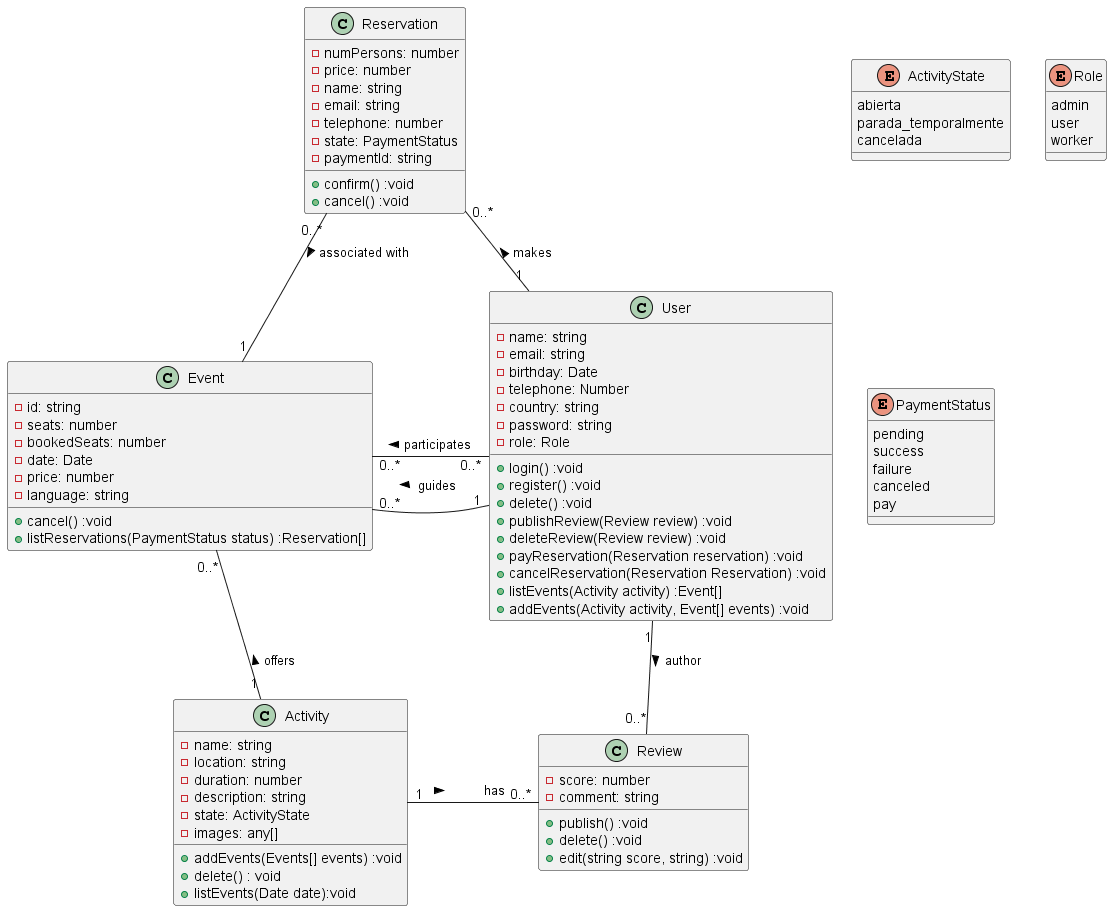
\includegraphics[width=1\textwidth]{5-AnalisisDelSistemaDeInformacion/Clases/diagrama.png}
	\caption{Diagrama de clases}
	\label{fig:mi_imagen}
\end{figure}

\subsection{Descripción de las clases}
A continuación, se detallan las clases correspondientes a los subsistemas de gestión de usuarios, actividades y reservas, cada una con una breve descripción, sus atributos y métodos propuestos.
\subsubsection{Subsistema de gestión de usuarios}
\begin{clases}
	\centering
	\begin{tabular}{|>{\raggedright\arraybackslash}p{4cm}|p{12cm}|}
		\hline
		\textbf{Nombre de la clase}   & \textbf{User}                                                                                                                                                                                                                                                          \\
		\hline
		\textbf{Descripción}          & Representa a un usuario del sistema, almacenando información personal como nombre, correo electrónico, fecha de nacimiento, y otros detalles de contacto. Los usuarios pueden tener roles diferentes que determinan sus permisos y acciones disponibles en el sistema. \\
		\hline
		\textbf{Atributos Propuestos} & \textbf{name}: string - Nombre del usuario.                                                                                                                                                                                                                            \\
		                              & \textbf{email}: string - Correo electrónico del usuario.                                                                                                                                                                                                               \\
		                              & \textbf{birthday}: Date - Fecha de nacimiento del usuario.                                                                                                                                                                                                             \\
		                              & \textbf{telephone}: Number - Número de teléfono del usuario.                                                                                                                                                                                                           \\
		                              & \textbf{country}: string - País de residencia del usuario.                                                                                                                                                                                                             \\
		                              & \textbf{password}: string - Contraseña de acceso del usuario.                                                                                                                                                                                                          \\
		                              & \textbf{role}: Role - Rol del usuario en el sistema (\textit{definido en el enum Role}).                                                                                                                                                                               \\
		\hline
		\textbf{Métodos Propuestos}   & \textbf{login(): void}                                                                                                                                                                                                                                                 \\
		                              & Permite al usuario iniciar sesión.                                                                                                                                                                                                                                     \\
		                              & \textbf{register(): void}                                                                                                                                                                                                                                              \\
		                              & Registra al usuario en el sistema.                                                                                                                                                                                                                                     \\
		                              & \textbf{delete(): void}                                                                                                                                                                                                                                                \\
		                              & Elimina la cuenta del usuario.                                                                                                                                                                                                                                         \\
		                              & \textbf{publishReview(Review review): void}                                                                                                                                                                                                                            \\
		                              & Publica una reseña.                                                                                                                                                                                                                                                    \\
		                              & \textbf{deleteReview(Review review): void}                                                                                                                                                                                                                             \\
		                              & Elimina una reseña.                                                                                                                                                                                                                                                    \\
		                              & \textbf{payReservation(Reservation reservation): void}                                                                                                                                                                                                                 \\
		                              & Realiza el pago de una reserva.                                                                                                                                                                                                                                        \\
		                              & \textbf{cancelReservation(Reservation reservation): void}                                                                                                                                                                                                              \\
		                              & Cancela una reserva.                                                                                                                                                                                                                                                   \\
		                              & \textbf{addEvents(Activity activity, Event[] events): void}                                                                                                                                                                                                            \\
		                              & Añade eventos a una actividad.                                                                                                                                                                                                                                         \\
		\hline
	\end{tabular}
	\caption{Clases - User}
\end{clases}
\subsubsection{Subsistema de gestión de actividades}
\begin{clases}
	\centering
\begin{tabular}{|>{\raggedright\arraybackslash}p{4cm}|p{12cm}|}
		\hline
		\textbf{Nombre de la clase}   & \textbf{Activity}                                                                                                                                                                                                                         \\
		\hline
		\textbf{Descripción}          & Representa una actividad ofrecida donde cada instancia incluye información detallada como ubicación, duración y una descripción. La clase gestiona los eventos asociados que pueden ocurrir en diferentes fechas o en diferentes idiomas. \\
		\hline
		\textbf{Atributos Propuestos} & \textbf{name}: string - Nombre de la actividad.                                                                                                                                                                                           \\
		                              & \textbf{location}: string - Ubicación de la actividad.                                                                                                                                                                                    \\
		                              & \textbf{duration}: number - Duración de la actividad.                                                                                                                                                                                     \\
		                              & \textbf{description}: string - Descripción de la actividad.                                                                                                                                                                               \\
		                              & \textbf{state}: ActivityState - Estado actual de la actividad (\textit{definido en el enum ActivityState}).                                                                                                                               \\
		                              & \textbf{images}: string[] - Imágenes relacionadas con la actividad.                                                                                                                                                                       \\
		\hline
		\textbf{Métodos Propuestos}   & \textbf{addEvents(Events[] events): void}                                                                                                                                                                                                 \\
		                              & Añade eventos a la actividad.                                                                                                                                                                                                             \\
		                              & \textbf{delete(): void}                                                                                                                                                                                                                   \\
		                              & Elimina la actividad.                                                                                                                                                                                                                     \\
		                              & \textbf{listEvents(Date date): void}                                                                                                                                                                                                      \\
		                              & Lista eventos según la fecha proporcionada.                                                                                                                                                                                               \\
		\hline
	\end{tabular}
	\caption{Clases - Activity}
\end{clases}

\begin{clases}
	\centering
\begin{tabular}{|>{\raggedright\arraybackslash}p{4cm}|p{12cm}|}
		\hline
		\textbf{Nombre de la clase}   & \textbf{Event}                                                                                                                                                                              \\
		\hline
		\textbf{Descripción}          & Encapsula los detalles de un evento específico asociado a una actividad. Esto incluye información sobre la capacidad de asientos, reservaciones realizadas, precio, y el idioma del evento. \\
		\hline
		\textbf{Atributos Propuestos} & \textbf{id}: string - Identificador único del evento.                                                                                                                                       \\
		                              & \textbf{seats}: number - Número total de asientos disponibles.                                                                                                                              \\
		                              & \textbf{bookedSeats}: number - Asientos reservados.                                                                                                                                         \\
		                              & \textbf{date}: Date - Fecha del evento.                                                                                                                                                     \\
		                              & \textbf{price}: number - Precio por asiento.                                                                                                                                                \\
		                              & \textbf{language}: string - Idioma en que se realiza el evento.                                                                                                                             \\
		\hline
		\textbf{Métodos Propuestos}   & \textbf{cancel(): void}                                                                                                                                                                     \\
		                              & Cancela el evento.                                                                                                                                                                          \\
		                              & \textbf{listReservations(PaymentStatus status): Reservation[]}                                                                                                                              \\
		                              & Lista las reservaciones basadas en su estado de pago.                                                                                                                                       \\

		\hline
	\end{tabular}
	\caption{Clases - Events}
\end{clases}

\begin{clases}
	\centering
\begin{tabular}{|>{\raggedright\arraybackslash}p{4cm}|p{12cm}|}
		\hline
		\textbf{Nombre de la clase}   & \textbf{Review}                                                                                                                                                                                    \\
		\hline
		\textbf{Descripción}          & Representa las reseñas que realizan los usuarios sobre las actividades. Actúa como un mecanismo para que los usuarios expresen su satisfacción o insatisfacción y mejoren la calidad de la oferta. \\
		\hline
		\textbf{Atributos Propuestos} & \textbf{score}: number - Puntuación otorgada a la actividad o evento.                                                                                                                              \\
		                              & \textbf{comment}: string - Comentario detallado sobre la experiencia.                                                                                                                              \\
		\hline
		\textbf{Métodos Propuestos}   & \textbf{publish(): void}                                                                                                                                                                           \\
		                              & Publica la reseña.                                                                                                                                                                                 \\
		                              & \textbf{delete(): void}                                                                                                                                                                            \\
		                              & Elimina la reseña.                                                                                                                                                                                 \\
		                              & \textbf{edit(string score, string comment): void}                                                                                                                                                  \\
		                              & Edita la reseña.                                                                                                                                                                                   \\
		\hline
	\end{tabular}
	\caption{Clases - Review}
\end{clases}
\subsubsection{Subsistema de gestión de reservas}
\begin{clases}
	\centering
\begin{tabular}{|>{\raggedright\arraybackslash}p{4cm}|p{12cm}|}
		\hline
		\textbf{Nombre de la clase}   & \textbf{Reservation}                                                                                                                                                                                                                                                                                                                                   \\
		\hline
		\textbf{Descripción}          & Representa las reservas hechas por los usuarios para los eventos. Cada reserva incluye detalles como el número de personas, el precio total, el estado del pago, y la identificación del evento reservado. Proporciona métodos para confirmar o cancelar reservas, y es crucial para la administración de la asistencia y los ingresos de los eventos. \\
		\hline
		\textbf{Atributos Propuestos} & \textbf{numPersons}: number - Número de personas para la reserva.                                                                                                                                                                                                                                                                                      \\
		                              & \textbf{price}: number - Precio total de la reserva.                                                                                                                                                                                                                                                                                                   \\
		                              & \textbf{name}: string - Nombre del usuario que realiza la reserva.                                                                                                                                                                                                                                                                                     \\
		                              & \textbf{email}: string - Correo electrónico del usuario que realiza la reserva.                                                                                                                                                                                                                                                                        \\
		                              & \textbf{telephone}: number - Número de teléfono del usuario que realiza la reserva.                                                                                                                                                                                                                                                                    \\
		                              & \textbf{state}: PaymentStatus - Estado del pago de la reserva (pendiente, éxito, fallo, cancelado, pago).                                                                                                                                                                                                                                              \\
		                              & \textbf{paymentId}: string - Identificador único del pago.                                                                                                                                                                                                                                                                                             \\
		\hline
		\textbf{Métodos Propuestos}   & \textbf{confirm(): void}                                                                                                                                                                                                                                                                                                                               \\
		                              & Confirma la reserva.                                                                                                                                                                                                                                                                                                                                   \\
		                              & \textbf{cancel(): void}                                                                                                                                                                                                                                                                                                                                \\
		                              & Cancela la reserva.                                                                                                                                                                                                                                                                                                                                    \\
		\hline
	\end{tabular}
	\caption{Clases - Reservation}
\end{clases}
\section{Definición de interfaces de usuario}
\subsection{Descripción de la interfaz }
En este apartado se mostrarán los bocetos que se han realizado para la interfaz de usuario de este proyecto. Las vistas sufren ligeras modificaciones dependiendo del rol que tenga el usuario, si está registrado o no, así como el dispositivo que se esté usando. Se han identificado las siguientes ventanas.
\subsubsection{Inicio}
La vista “Inicio” será aquella que se vea nada más acceder a la aplicación. En ella se pondrá observar la lista de actividades más populares así como un botón para poder ir directamente a la búsqueda de actividades.
\begin{figure}[H]
	\centering
	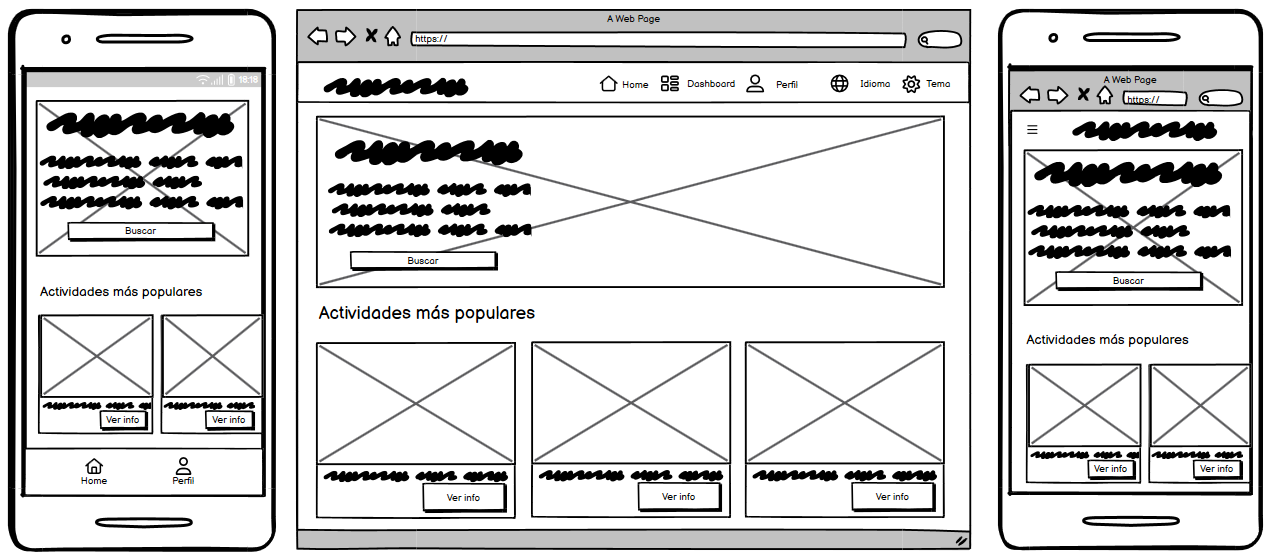
\includegraphics[width=0.8\textwidth]{5-AnalisisDelSistemaDeInformacion/InterfacesDeUsuario/Inicio/inicio-admin.png}
	\caption{Inicio - Vista Administrador }
\end{figure}

\begin{figure}[H]
	\centering
	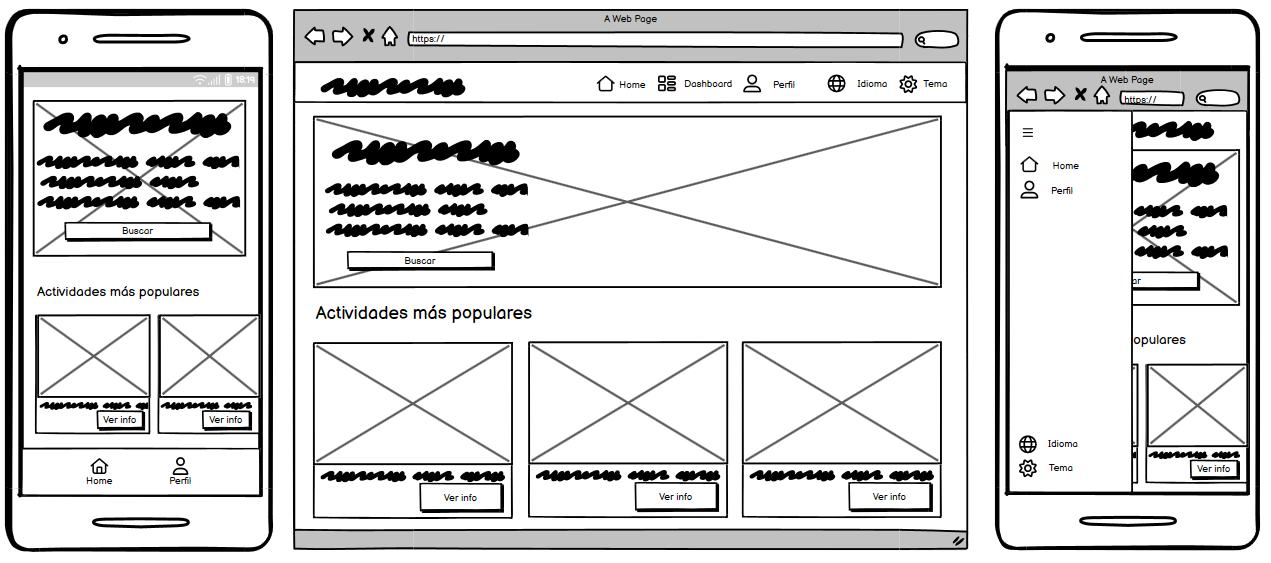
\includegraphics[width=0.8\textwidth]{5-AnalisisDelSistemaDeInformacion/InterfacesDeUsuario/Inicio/inicio-admin-menu.png}
	\caption{Inicio - Vista Administrador (Menú desplegado)}
\end{figure}

\begin{figure}[H]
	\centering
	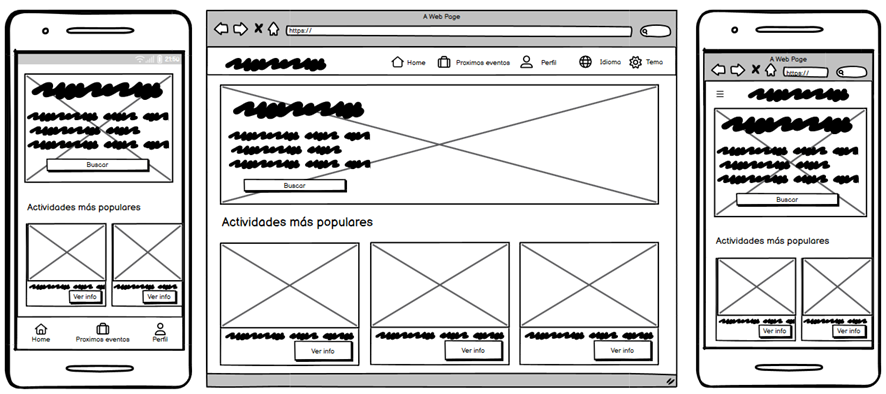
\includegraphics[width=0.8\textwidth]{5-AnalisisDelSistemaDeInformacion/InterfacesDeUsuario/Inicio/inicio-guia.png}
	\caption{Inicio - Vista Guía }
\end{figure}

\begin{figure}[H]
	\centering
	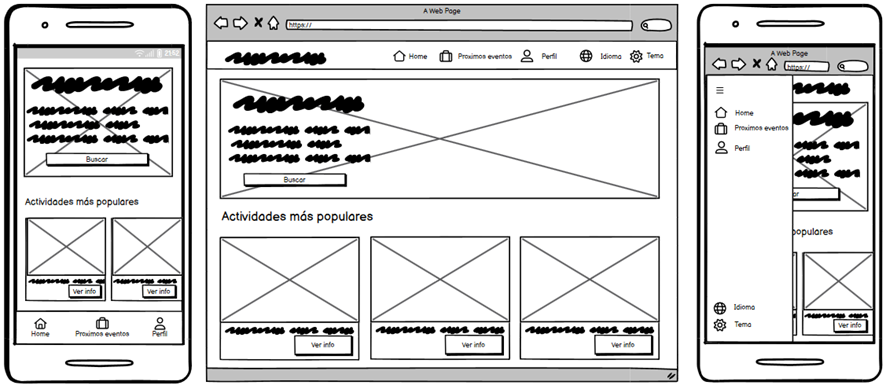
\includegraphics[width=0.8\textwidth]{5-AnalisisDelSistemaDeInformacion/InterfacesDeUsuario/Inicio/inicio-guia-menu.png}
	\caption{Inicio - Vista Guía (Menú desplegado)}
\end{figure}

\begin{figure}[H]
	\centering
	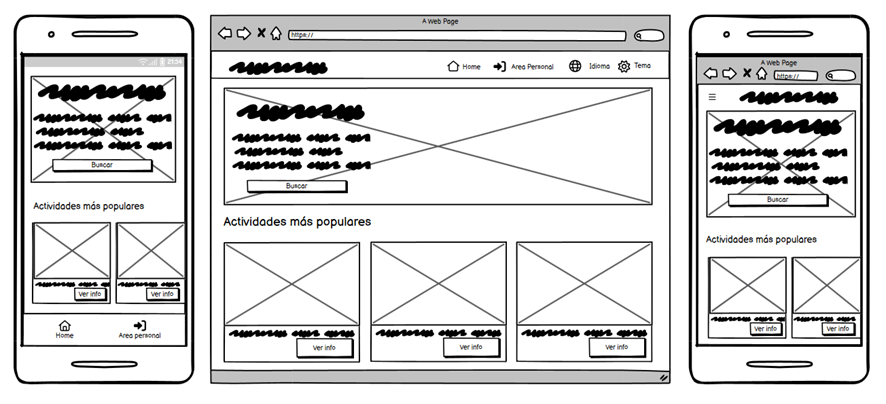
\includegraphics[width=0.8\textwidth]{5-AnalisisDelSistemaDeInformacion/InterfacesDeUsuario/Inicio/inicio-no-identificado.png}
	\caption{Inicio - Vista Usuario no identificado }
\end{figure}

\begin{figure}[H]
	\centering
	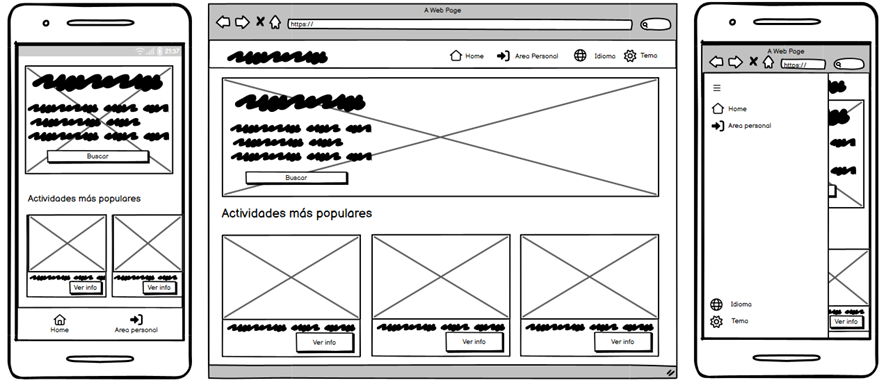
\includegraphics[width=0.8\textwidth]{5-AnalisisDelSistemaDeInformacion/InterfacesDeUsuario/Inicio/inicio-no-identificado-menu.png}
	\caption{Inicio - Vista Usuario no identificado (Menú desplegado)}
\end{figure}

\begin{figure}[H]
	\centering
	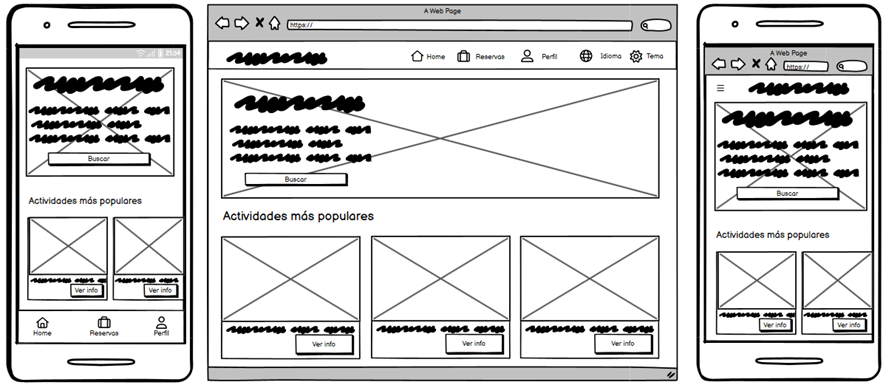
\includegraphics[width=0.8\textwidth]{5-AnalisisDelSistemaDeInformacion/InterfacesDeUsuario/Inicio/inicio-turista.png}
	\caption{Inicio - Vista Turista }
\end{figure}

\begin{figure}[H]
	\centering
	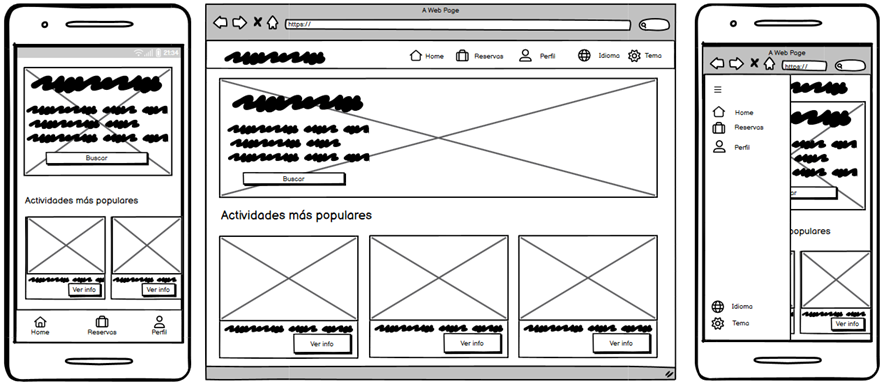
\includegraphics[width=0.8\textwidth]{5-AnalisisDelSistemaDeInformacion/InterfacesDeUsuario/Inicio/inicio-turista-menu.png}
	\caption{Inicio - Vista Turista (Menú desplegado)}
\end{figure}

\subsubsection{Inicio de sesión}
La vista “Inicio de sesión” será aquella vista que se enseñará cuando el usuario quiera identificarse en la aplicación.
En esta vista el usuario podrá introducir su correo electrónico y contraseña para poder acceder a la aplicación.
\begin{figure}[H]
	\centering
	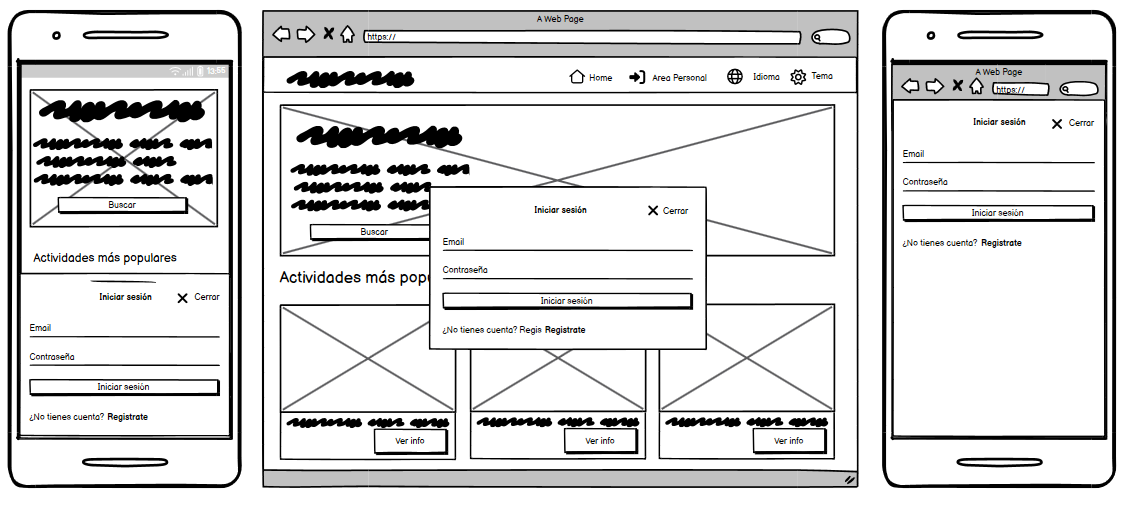
\includegraphics[width=0.8\linewidth]{5-AnalisisDelSistemaDeInformacion/InterfacesDeUsuario/InicioDeSesion/inicioDeSesion.png}
	\caption{Inicio de sesión}
\end{figure}
\subsubsection{Registro}
La vista “Registro” será aquella vista que se enseñará cuando el usuario quiera registrarse en la aplicación.
En esta vista el usuario deberá introducir sus datos personales y una contraseña.
\begin{figure}[H]
	\centering
	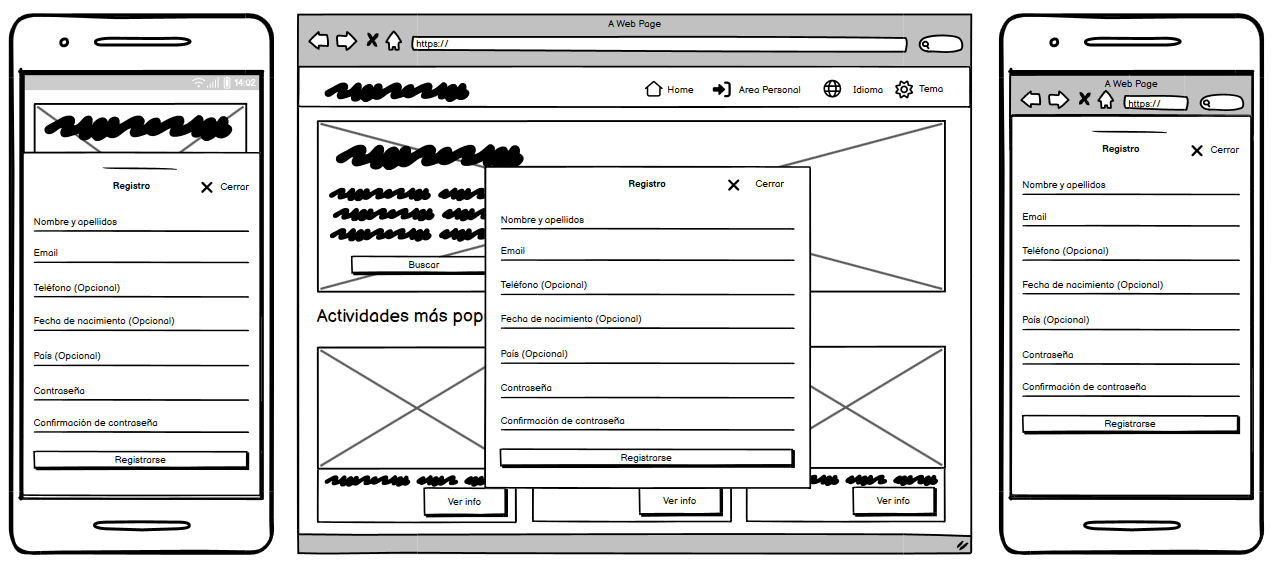
\includegraphics[width=0.8\linewidth]{5-AnalisisDelSistemaDeInformacion/InterfacesDeUsuario/Registro/registro.png}
	\caption{Registro}
\end{figure}
\subsubsection{Buscar actividades}
La vista “Buscar actividades” será aquella vista que se enseñará cuando el usuario quiera hacer una búsqueda de las actividades. En esta búsqueda el usuario podrá aplicar filtros y ordenar los resultados según el criterio que más le convenga.
\begin{figure}[H]
	\centering
	\includegraphics[width=0.8\linewidth]{5-AnalisisDelSistemaDeInformacion/InterfacesDeUsuario/BuscarActividades/buscar-standar.png}
	\caption{Buscar Actividades}
\end{figure}

\begin{figure}[H]
	\centering
	\includegraphics[width=0.8\linewidth]{5-AnalisisDelSistemaDeInformacion/InterfacesDeUsuario/BuscarActividades/buscar-standar-aplicando-filtros.png}
	\caption{Buscar Actividades - Aplicar Filtros}
\end{figure}

\begin{figure}[H]
	\centering
	\includegraphics[width=0.8\linewidth]{5-AnalisisDelSistemaDeInformacion/InterfacesDeUsuario/BuscarActividades/buscar-standar-borrar-filtros.png}
	\caption{Buscar Actividades - Borrar Filtros}
\end{figure}

\begin{figure}[H]
	\centering
	\includegraphics[width=0.8\linewidth]{5-AnalisisDelSistemaDeInformacion/InterfacesDeUsuario/BuscarActividades/buscar-standar-con-filtros.png}
	\caption{Buscar Actividades - Con Filtros}
\end{figure}


\subsubsection{Detalles de actividad}
La vista “Detalles de actividad” será aquella vista que se enseñará cuando el usuario quiera ver la información asociada a la actividad. En esta vista el usuario también podrá ver las valoraciones y la disponibilidad en caso de que la actividad tenga eventos con plazas disponibles.
\begin{figure}[H]
	\centering
	\includegraphics[width=0.8\textwidth]{5-AnalisisDelSistemaDeInformacion/InterfacesDeUsuario/Detalles de actividad/detalles-estandar.png}
	\caption{Detalles de actividad}
\end{figure}

\begin{figure}[H]
	\centering
	\includegraphics[width=0.8\textwidth]{5-AnalisisDelSistemaDeInformacion/InterfacesDeUsuario/Detalles de actividad/detalles-estandar-disponibilidad.png}
	\caption{Detalles de actividad - Disponibilidad}
\end{figure}
\subsubsection{Realizar reserva}
La vista “Realizar reserva” será aquella vista que se enseñará cuando el usuario quiera empiece el proceso de compra. En esta vista el usuario pasará por distintos pasos donde deberá introducir datos personales y datos bancarios para realizar la reserva.
\begin{figure}[H]
	\centering
	\includegraphics[width=0.8\linewidth]{5-AnalisisDelSistemaDeInformacion/InterfacesDeUsuario/Reservar/reservar-paso1.png}
	\caption{Realizar reserva - Paso 1: Selección de opciones}
	\label{fig:paso1}
\end{figure}

\begin{figure}[H]
	\centering
	\includegraphics[width=0.8\linewidth]{5-AnalisisDelSistemaDeInformacion/InterfacesDeUsuario/Reservar/reservar-paso2-personales.png}
	\caption{Realizar reserva - Paso 2: Información personal}
	\label{fig:paso2-personales}
\end{figure}

\begin{figure}[H]
	\centering
	\includegraphics[width=0.8\linewidth]{5-AnalisisDelSistemaDeInformacion/InterfacesDeUsuario/Reservar/reservar-paso2-bancarios.png}
	\caption{Realizar reserva - Paso 2: Información bancaria}
	\label{fig:paso2-bancarios}
\end{figure}

\begin{figure}[H]
	\centering
	\includegraphics[width=0.8\linewidth]{5-AnalisisDelSistemaDeInformacion/InterfacesDeUsuario/Reservar/reservar-paso3.png}
	\caption{Realizar reserva - Paso 3: Confirmación}
	\label{fig:paso3}
\end{figure}
\subsubsection{Lista de reservas}
En esta vista “Lista de reservas” el usuario podrá ver todas las reservas realizadas agrupadas por rangos de fechas próximas.
\begin{figure}[H]
	\centering
	\includegraphics[width=0.8\linewidth]{5-AnalisisDelSistemaDeInformacion/InterfacesDeUsuario/Lista de reservas/lista.png}
	\caption{Lista de reservas}
\end{figure}
\subsubsection*{Gestión de reserva}
En esta vista “Gestión de reserva” el usuario podrá ver la información asociada a la reserva, añadir una reseña si ha completado la reserva, así como cancelarla si lo desea.
\begin{figure}[H]
	\centering
	\includegraphics[width=0.8\textwidth]{5-AnalisisDelSistemaDeInformacion/InterfacesDeUsuario/Detalles de reserva/detalles.png}
	\caption{Gestión de reserva}
\end{figure}
\subsubsection{Perfil}
En esta vista “Perfil” el usuario podrá ver todos sus datos personales, asi como gestionar su cuenta, ya sea para cambiar la contraseña o para cancelar la cuenta.
\begin{figure}[H]
	\centering
	\includegraphics[width=0.8\linewidth]{5-AnalisisDelSistemaDeInformacion/InterfacesDeUsuario/Perfil/perfil-personales.png}
	\caption{Perfil - Datos Personales}
\end{figure}

\begin{figure}[H]
	\centering
	\includegraphics[width=0.8\linewidth]{5-AnalisisDelSistemaDeInformacion/InterfacesDeUsuario/Perfil/perfil-cuenta.png}
	\caption{Perfil - Cuenta}
\end{figure}

\begin{figure}[H]
	\centering
	\includegraphics[width=0.8\linewidth]{5-AnalisisDelSistemaDeInformacion/InterfacesDeUsuario/Perfil/perfil-cambio-personales.png}
	\caption{Perfil - Cambio de Datos Personales}
\end{figure}

\begin{figure}[H]
	\centering
	\includegraphics[width=0.8\linewidth]{5-AnalisisDelSistemaDeInformacion/InterfacesDeUsuario/Perfil/perfil-cambio-contraseña.png}
	\caption{Perfil - Cambio de Contraseña}
\end{figure}
\subsubsection{Dashboard}
En esta vista “Dashboard” el usuario registrado como administrador podrá ver los datos estadísticos de la aplicación, así como gestionar las actividades y los usuarios.
\begin{figure}[H]
	\centering
	\includegraphics[width=0.8\textwidth]{5-AnalisisDelSistemaDeInformacion/InterfacesDeUsuario/Dashboard/panel de control.png}
	\caption{Dashboard - Panel de control}
\end{figure}


En el apartado “Usuarios” de la vista “Dashboard” se muestra una lista de los usuarios registrados en el sistema.
En la tabla se muestra el nombre, correo electrónico, el rol y las reservas realizadas de cada usuario.
Además, se incluye un botón para ver los detalles de cada usuario que nos llevará a la vista “Detalles de usuario” .

\begin{figure}[H]
	\centering
	\includegraphics[width=0.8\textwidth]{5-AnalisisDelSistemaDeInformacion/InterfacesDeUsuario/Dashboard/lista usuarios.png}
	\caption{Dashboard - Lista de usuarios}
\end{figure}

\begin{figure}[H]
	\centering
	\includegraphics[width=0.8\textwidth]{5-AnalisisDelSistemaDeInformacion/InterfacesDeUsuario/Dashboard/lista usuarios edit.png}
	\caption{Dashboard - Editar usuario}
\end{figure}

En el apartado “Actividades” de la vista “Dashboard” se muestra una lista de las actividades registradas en el sistema.
En la tabla se muestra el nombre, fecha de inicio, fecha de fin, lugar, descripción y el estado de cada actividad.
En caso de querer ver los eventos de una actividad, se puede hacer clic en la opción del menú lateral “Mostrar eventos” .

\begin{figure}[H]
	\centering
	\includegraphics[width=0.8\textwidth]{5-AnalisisDelSistemaDeInformacion/InterfacesDeUsuario/Dashboard/lista de actividades.png}
	\caption{Dashboard - Lista de actividades}
\end{figure}

\begin{figure}[H]
	\centering
	\includegraphics[width=0.8\textwidth]{5-AnalisisDelSistemaDeInformacion/InterfacesDeUsuario/Dashboard/lista de actividades edit.png}
	\caption{Dashboard - Lista de actividades}
\end{figure}

\begin{figure}[H]
	\centering
	\includegraphics[width=0.8\textwidth]{5-AnalisisDelSistemaDeInformacion/InterfacesDeUsuario/Dashboard/lista eventos.png}
	\caption{Dashboard - Lista de actividades con eventos}
\end{figure}

\begin{figure}[H]
	\centering
	\includegraphics[width=0.8\textwidth]{5-AnalisisDelSistemaDeInformacion/InterfacesDeUsuario/Dashboard/lista eventos edit.png}
	\caption{Dashboard - Editar evento}
\end{figure}

\subsubsection*{Detalles de usuario}
En la vista “Detalles de usuario” se muestra la información personal de un usuario, así como las reservas realizadas por el mismo.
Además, se incluye un botón para editar los datos del usuario y otro para editar una reserva.

\begin{figure}[H]
	\centering
	\includegraphics[width=0.8\textwidth]{5-AnalisisDelSistemaDeInformacion/InterfacesDeUsuario/Dashboard/detalles usuario.png}
	\caption{Detalles de usuario}
\end{figure}

\begin{figure}[H]
	\centering
	\includegraphics[width=0.8\textwidth]{5-AnalisisDelSistemaDeInformacion/InterfacesDeUsuario/Dashboard/detalles usuario editar datos.png}
	\caption{Detalles de usuario - Editar datos}
\end{figure}

\begin{figure}[H]
	\centering
	\includegraphics[width=0.8\textwidth]{5-AnalisisDelSistemaDeInformacion/InterfacesDeUsuario/Dashboard/detalles usuario editar reserva.png}
	\caption{Detalles de usuario - Editar reserva}
\end{figure}

\subsubsection{Eventos próximos}
En esta vista “Eventos próximos” el usuario registrado como guía podrá ver los eventos que tiene próximamente planificados, así como información de contacto de los turistas que han reservado.
\begin{figure}[H]
	\centering
	\includegraphics[width=0.8\textwidth]{5-AnalisisDelSistemaDeInformacion/InterfacesDeUsuario/EventosProximos/eventos proximos.png}
	\caption{Eventos próximos}
\end{figure}

\begin{figure}[H]
	\centering
	\includegraphics[width=0.8\textwidth]{5-AnalisisDelSistemaDeInformacion/InterfacesDeUsuario/EventosProximos/eventos proximos participantes.png}
	\caption{Eventos próximos - Participantes}
\end{figure}

\subsection{Descripción del comportamiento de la interfaz}
\subsubsection{Diagrama de navegabilidad}
A continuación se presenta el diagrama de navegabilidad, que ilustra las relaciones y transiciones entre las diferentes páginas y componentes de la interfaz
\begin{figure}[H]
	\centering
	\includegraphics[width=1\linewidth]{5-AnalisisDelSistemaDeInformacion/Navegabilidad/diagrama.png}
	\caption{Diagrama de las relaciones entre los subsistemas}
	\label{fig:diagrama}
\end{figure}
\section{Especificación del plan de pruebas}
En esta sección se describe el plan de pruebas que se llevará a cabo para garantizar la calidad y funcionalidad del sistema. Se realizarán pruebas unitarias, pruebas de integración y pruebas de usabilidad.
\subsection{Pruebas unitarias}
Las pruebas unitarias se centran en validar el correcto funcionamiento de cada componente individual del sistema. Para ello:
\begin{itemize}
	\item Se definirán casos de prueba específicos para cada función o método.
	\item Cada caso de prueba verificará que los resultados obtenidos sean los esperados bajo diferentes condiciones.
	\item Se empleará el framework de pruebas unitarias Jest, conocido por su eficacia en la detección de errores en etapas tempranas del desarrollo.
	\item Estas pruebas se ejecutarán de manera automatizada para asegurar la repetibilidad y consistencia de los resultados.
\end{itemize}
\subsection{Pruebas de integración}
Para verificar la correcta integración entre los diferentes módulos de la funcionalidad de reservas de actividades, se realizarán pruebas de integración centradas en la creación de reservas, dado que es la funcionalidad principal y la que más relaciones entre módulos presenta.
Las pruebas se llevarán a cabo en un entorno de pruebas similar al de producción utilizando herramientas de automatización como Cypress.
Se comprobará la conexión entre el módulo de usuario y el módulo de reservas para asegurar que un usuario autenticado puede crear una reserva;
la conexión entre el módulo de actividades y el módulo de reservas para verificar que las actividades disponibles se cargan y pueden ser seleccionadas correctamente;
y la interacción entre el módulo de reservas y la base de datos para garantizar que la información de la reserva se almacena y recupera adecuadamente.

Además se realizarán pruebas manuales para comprobar la correcta visualización de la información de la reserva en la interfaz de usuario y la correcta actualización de la base de datos tras la realización de una reserva.
\subsection{Pruebas de usabilidad}
Las pruebas de usabilidad están diseñadas para evaluar la experiencia del usuario al interactuar con el sistema. Estas pruebas se centrarán en la facilidad de uso, la eficiencia y la satisfacción del usuario. El enfoque principal será la realización de un cuestionario estructurado después de que los participantes completen una serie de tareas específicas en la aplicación. A continuación se detalla el plan para estas pruebas:
\\[1ex]
\textbf{Selección de Participantes:}
\\[1ex]
Se seleccionarán de 3 a 5 personas que representen el público objetivo de la aplicación.
Los participantes deben tener diferentes niveles de experiencia con aplicaciones similares para obtener una variedad de perspectivas.
Tareas a Realizar:
\begin{enumerate}
	\item Registrarse en la aplicación
	\item Cerrar sesión
	\item Iniciar sesión
	\item Buscar actividades
	\item Filtrar actividades por texto
	\item Filtrar actividades por rango/precio/personas
	\item Borrar filtros de búsqueda
	\item Ver Detalles de una actividad
	\item Reservar una actividad
	\item Cancelar una reserva
	\item Añadir una valoración
	\item Editar una valoración
	\item Eliminar una valoración
	\item Ver datos personales
	\item Editar datos personales
	\item Cambiar la contraseña
	\item Cambiar el tema de la aplicación
	\item Cambiar el idioma de la aplicación
	\item Eliminar la cuenta
\end{enumerate}

Al ser una aplicación web y móvil, se realizarán pruebas en ambas plataformas para evaluar la consistencia y la usabilidad en diferentes dispositivos.
A su vez, también se evaluarán tareas de administración para los usuarios con rol de administrador y tareas de guía para los usuarios con rol de guía.

\textbf{Cuestionario de Usabilidad:}
\\[1ex]
Después de completar cada tarea, los participantes responderán a preguntas sobre la facilidad de realizar la tarea y cualquier problema que hayan encontrado.
Se recopilará feedback cualitativo y cuantitativo para evaluar la usabilidad general de la aplicación.
\chapter{Diseño del sistema de información}
\section{Diseño de casos de uso reales}
Esta sección presenta el diseño de los casos de uso más relevantes para el sistema. A continuación, se muestran diagramas de secuencia que ilustran las interacciones entre el usuario y los distintos componentes del sistema.
\subsection{Caso de uso: Crear cuenta}
Este caso de uso abarca todos los pasos necesarios, desde la entrada de datos por parte del usuario hasta la confirmación de la creación de la cuenta.
\\[1ex]A continuación, se detalla el flujo de interacción entre los diferentes actores y componentes del sistema mediante un diagrama de secuencia.
\begin{figure}[H]
	\centering
	\includegraphics[width=1\linewidth]{6-DiseñoDelSistemaDeInformacion/CasosDeUso/CrearCuenta/crear-cuenta.png}
	\caption{Diagrama de secuencia: Crear cuenta.}
\end{figure}
\subsection{Caso de uso: Inicio de sesión}
Este caso de uso detalla las interacciones necesarias entre el usuario y los componentes del sistema para autenticar al usuario de manera segura y eficiente.
\\[1ex]A continuación, se presenta el diagrama de secuencia que describe estas interacciones.
\begin{figure}[H]
	\centering
	\includegraphics[width=1\linewidth]{6-DiseñoDelSistemaDeInformacion/CasosDeUso/InicioDeSesion/inicio-de-sesion.png}
	\caption{Diagrama de secuencia: Inicio de sesión.}
\end{figure}
\subsection{Caso de uso: Buscar actividades}
Este caso de uso describe las interacciones necesarias para que el usuario pueda buscar actividades en la aplicación.
\\[1ex]A continuación, se presenta el diagrama de secuencia que describe estas interacciones.
\begin{figure}[H]
	\centering
	\includegraphics[width=1\linewidth]{6-DiseñoDelSistemaDeInformacion/CasosDeUso/BuscarActividades/buscar-actividades.png}
	\caption{Diagrama de secuencia: Buscar actividades.}
\end{figure}
\subsection{Caso de uso: Crear una reserva}
Este caso de uso muestra las interacciones necesarias para que el usuario pueda realizar una reserva en la aplicación.
\\[1ex]A continuación, se presenta el diagrama de secuencia que describe estas interacciones.
\begin{figure}[H]
	\centering
	\begin{adjustwidth}{-0.7cm}{}
		\includegraphics[width=1.05\linewidth]{6-DiseñoDelSistemaDeInformacion/CasosDeUso/CrearReserva/crear-reserva.png}
	\end{adjustwidth}
	\caption{Diagrama de secuencia: Crear reserva.}
\end{figure}

% \subsubsection{Diagrama de estados}
% \begin{figure}[H]
	\centering
	\includegraphics[width=1.05\linewidth]{6-DiseñoDelSistemaDeInformacion/CasosDeUso/CrearReserva/estados-reserva.png}
	\caption{Diagrama de estados: Reserva.}
\end{figure}
\section{Diseño de clases}
\subsection{Diagrama de clases}
\input{6-DiseñoDelSistemaDeInformacion/diagrama-de-clases.tex}
\section{Diseño de la arquitectura de módulos del sistema}
\subsection{Diseño de módulos del sistema}
\subsubsection{Módulo del cliente}
El módulo del cliente se compone de varios paquetes esenciales, cada uno con un rol específico en la estructura del sistema:
\begin{itemize}
	\item \textbf{Componentes:}  Este paquete contiene todos los componentes de la interfaz de usuario que se componen para formar las diferentes vistas de la aplicación.
	\item \textbf{Layouts:} Define la estructura general de las páginas, utilizando componentes y temas para asegurar una apariencia consistente en toda la aplicación.
	\item \textbf{Tema:} Se utiliza para aplicar estilos y temas consistentes a los componentes y layouts, asegurando una experiencia de usuario uniforme.
	\item \textbf{Hooks:} Almacena la lógica reutilizable que puede ser compartida entre diferentes componentes. Utiliza APIs y contextos para manejar datos y estados.
	\item \textbf{APIs:} Gestiona la comunicación con el servidor, realizando llamadas a las diferentes APIs necesarias para la funcionalidad de la aplicación.
	\item \textbf{Contextos:} Proporciona un mecanismo para compartir estados y datos entre componentes sin necesidad de pasar props manualmente en cada nivel.
\end{itemize}
El diagrama también muestra cómo el cliente se comunica con el servidor, asegurando que los datos fluyan correctamente entre el frontend y el backend.

\begin{figure}[H]
	\centering
	\includegraphics[width=1\linewidth]{6-DiseñoDelSistemaDeInformacion/Modulos/cliente.png}
	\caption{Diagrama de paquetes del Cliente}
\end{figure}
\subsubsection{Módulo del servidor}
El módulo del servidor se encarga de gestionar la lógica de negocio y la comunicación con la base de datos. A continuación, se presenta el diagrama de paquetes del servidor, que muestra la organización de sus componentes y la interacción entre ellos.
\\[1ex]
El servidor está compuesto por los siguientes paquetes:
\begin{itemize}
	\item \textbf{API:} Define la interfaz de comunicación entre el cliente y el servidor, especificando los endpoints disponibles.
	\item \textbf{Rutas:} Maneja la definición y el manejo de las rutas que el servidor expone, asociando cada ruta a su controlador correspondiente.
	\item \textbf{Middlewares:} Aplica funciones intermedias en la cadena de solicitudes HTTP, como autenticación, validación de datos y manejo de errores.
	\item \textbf{Controladores:} Contienen la lógica que maneja las solicitudes del cliente, delegando tareas específicas a los servicios y middlewares.
	\item \textbf{Servicios:} Implementan la lógica de negocio, realizando operaciones complejas y coordinando la interacción entre controladores y modelos.
	\item \textbf{Modelos:} Interactúan con la base de datos, definiendo la estructura de los datos y proporcionando métodos para su manipulación.
\end{itemize}

El diagrama también muestra cómo el cliente se comunica con la API del servidor y cómo el servidor maneja las solicitudes a través de sus componentes hasta llegar a la base de datos y viceversa.

\begin{figure}[H]
	\centering
	\includegraphics[width=1\linewidth]{6-DiseñoDelSistemaDeInformacion/Modulos/servidor.png}
	\caption{Diagrama de paquetes del Servidor}
\end{figure}
\subsection{Diseño de comunicaciones entre módulos}
\subsubsection{Diagrama de despliegue}
El diagrama de despliegue ilustra la arquitectura de la comunicación entre los módulos del sistema, destacando las conexiones y protocolos utilizados:
\begin{itemize}
	\item \textbf{Usuario:} Los usuarios acceden al sistema a través de dispositivos que pueden ser aplicaciones móviles (App) o navegadores web (Browser). La comunicación se realiza mediante el protocolo HTTPS en el puerto 443 para garantizar la seguridad de los datos transmitidos.
	\item \textbf{Servidor Web:} Este componente, desplegado en la nube, aloja la página web de la aplicación. Se encarga de servir las interfaces de usuario y manejar las solicitudes HTTPS provenientes de los clientes.
	\item \textbf{Servidor (AWS EC2):} El servidor principal está desplegado en un servicio EC2 de AWS. Este servidor maneja la lógica de negocio y procesa las solicitudes de los usuarios, comunicándose con la base de datos para acceder y manipular la información necesaria.
	\item \textbf{Base de Datos (MongoDB Atlas):} La base de datos está alojada en MongoDB Atlas, un servicio de base de datos en la nube. Este componente almacena todos los datos del sistema, organizados en esquemas como “Actividades” y “Usuarios”. La comunicación entre el servidor y la base de datos se realiza a través de una URI segura.
\end{itemize}

El diagrama también muestra cómo el servidor web y el servidor principal (EC2) se comunican con la base de datos en MongoDB Atlas.

\begin{figure}[H]
	\centering
	\includegraphics[width=1\linewidth]{6-DiseñoDelSistemaDeInformacion/Modulos/comunicaciones.png}
	\caption{Diagrama de despliegue}
\end{figure}

\section{Revisión de la interfaz de usuario}
\subsubsection{Inicio}
La vista “Inicio” será aquella que se vea nada más acceder a la aplicación. En ella se pondrá observar la lista de actividades más populares así como un botón para poder ir directamente a la búsqueda de actividades.
\begin{figure}[H]
	\centering
	\includegraphics[width=0.18\textwidth]{6-DiseñoDelSistemaDeInformacion/RevisionInterfaces/Inicio/inicio-admin-app.png}
	\includegraphics[width=0.5\textwidth]{6-DiseñoDelSistemaDeInformacion/RevisionInterfaces/Inicio/inicio-admin.png}
	\includegraphics[width=0.18\textwidth]{6-DiseñoDelSistemaDeInformacion/RevisionInterfaces/Inicio/inicio-admin-mobile.png}
	\caption{Inicio - Vista Administrador }
\end{figure}

\begin{figure}[H]
	\centering
	\includegraphics[width=0.18\textwidth]{6-DiseñoDelSistemaDeInformacion/RevisionInterfaces/Inicio/inicio-admin-app.png}
	\includegraphics[width=0.5\textwidth]{6-DiseñoDelSistemaDeInformacion/RevisionInterfaces/Inicio/inicio-admin.png}
	\includegraphics[width=0.18\textwidth]{6-DiseñoDelSistemaDeInformacion/RevisionInterfaces/Inicio/inicio-admin-menu.png}
	\caption{Inicio - Vista Administrador (Menú desplegado)}
\end{figure}

\begin{figure}[H]
	\centering
	\includegraphics[width=0.18\textwidth]{6-DiseñoDelSistemaDeInformacion/RevisionInterfaces/Inicio/inicio-guia-app.png}
	\includegraphics[width=0.5\textwidth]{6-DiseñoDelSistemaDeInformacion/RevisionInterfaces/Inicio/inicio-guia.png}
	\includegraphics[width=0.18\textwidth]{6-DiseñoDelSistemaDeInformacion/RevisionInterfaces/Inicio/inicio-admin-mobile.png}
	\caption{Inicio - Vista Guía }
\end{figure}

\begin{figure}[H]
	\centering
	\includegraphics[width=0.18\textwidth]{6-DiseñoDelSistemaDeInformacion/RevisionInterfaces/Inicio/inicio-guia-app.png}
	\includegraphics[width=0.5\textwidth]{6-DiseñoDelSistemaDeInformacion/RevisionInterfaces/Inicio/inicio-guia.png}
	\includegraphics[width=0.18\textwidth]{6-DiseñoDelSistemaDeInformacion/RevisionInterfaces/Inicio/inicio-guia-menu.png}
	\caption{Inicio - Vista Guía (Menú desplegado)}
\end{figure}

\begin{figure}[H]
	\centering
	\includegraphics[width=0.18\textwidth]{6-DiseñoDelSistemaDeInformacion/RevisionInterfaces/Inicio/inicio-no-identificado-app.png}
	\includegraphics[width=0.5\textwidth]{6-DiseñoDelSistemaDeInformacion/RevisionInterfaces/Inicio/inicio-no-identificado.png}
	\includegraphics[width=0.18\textwidth]{6-DiseñoDelSistemaDeInformacion/RevisionInterfaces/Inicio/inicio-admin-mobile.png}
	\caption{Inicio - Vista Usuario no identificado }
\end{figure}

\begin{figure}[H]
	\centering
	\includegraphics[width=0.18\textwidth]{6-DiseñoDelSistemaDeInformacion/RevisionInterfaces/Inicio/inicio-no-identificado-app.png}
	\includegraphics[width=0.5\textwidth]{6-DiseñoDelSistemaDeInformacion/RevisionInterfaces/Inicio/inicio-no-identificado.png}
	\includegraphics[width=0.18\textwidth]{6-DiseñoDelSistemaDeInformacion/RevisionInterfaces/Inicio/inicio-no-identificado-menu.png}
	\caption{Inicio - Vista Usuario no identificado (Menú desplegado)}
\end{figure}

\begin{figure}[H]
	\centering
	\includegraphics[width=0.18\textwidth]{6-DiseñoDelSistemaDeInformacion/RevisionInterfaces/Inicio/inicio-turista-app.png}
	\includegraphics[width=0.5\textwidth]{6-DiseñoDelSistemaDeInformacion/RevisionInterfaces/Inicio/inicio-turista.png}
	\includegraphics[width=0.18\textwidth]{6-DiseñoDelSistemaDeInformacion/RevisionInterfaces/Inicio/inicio-admin-mobile.png}
	\caption{Inicio - Vista Turista }
\end{figure}

\begin{figure}[H]
	\centering
	\includegraphics[width=0.18\textwidth]{6-DiseñoDelSistemaDeInformacion/RevisionInterfaces/Inicio/inicio-turista-app.png}
	\includegraphics[width=0.5\textwidth]{6-DiseñoDelSistemaDeInformacion/RevisionInterfaces/Inicio/inicio-turista.png}
	\includegraphics[width=0.18\textwidth]{6-DiseñoDelSistemaDeInformacion/RevisionInterfaces/Inicio/inicio-turista-menu.png}
	\caption{Inicio - Vista Turista (Menú desplegado)}
\end{figure}

\subsubsection{Buscar actividades}
La vista “Buscar actividades” será aquella vista que se enseñará cuando el usuario quiera hacer una búsqueda de las actividades. En esta búsqueda el usuario podrá aplicar filtros y ordenar los resultados según el criterio que más le convenga.
\begin{figure}[H]
	\centering
	\includegraphics[width=0.18\linewidth]{6-DiseñoDelSistemaDeInformacion/RevisionInterfaces/BuscarActividades/buscar-app.png}
	\includegraphics[width=0.5\linewidth]{6-DiseñoDelSistemaDeInformacion/RevisionInterfaces/BuscarActividades/buscar.png}
	\includegraphics[width=0.18\linewidth]{6-DiseñoDelSistemaDeInformacion/RevisionInterfaces/BuscarActividades/buscar-mobile.png}
	\caption{Buscar Actividades}
\end{figure}

\begin{figure}[H]
	\centering
	\includegraphics[width=0.18\linewidth]{6-DiseñoDelSistemaDeInformacion/RevisionInterfaces/BuscarActividades/buscar-aplicando-app.png}
	\includegraphics[width=0.5\linewidth]{6-DiseñoDelSistemaDeInformacion/RevisionInterfaces/BuscarActividades/buscar-borrando.png}
	\includegraphics[width=0.18\linewidth]{6-DiseñoDelSistemaDeInformacion/RevisionInterfaces/BuscarActividades/buscar-aplicando-mobile.png}
	\caption{Buscar Actividades - Aplicar Filtros}
\end{figure}

\begin{figure}[H]
	\centering
	\includegraphics[width=0.18\linewidth]{6-DiseñoDelSistemaDeInformacion/RevisionInterfaces/BuscarActividades/buscar-con-filtros-app.png}
	\includegraphics[width=0.5\linewidth]{6-DiseñoDelSistemaDeInformacion/RevisionInterfaces/BuscarActividades/buscar-borrando.png}
	\includegraphics[width=0.18\linewidth]{6-DiseñoDelSistemaDeInformacion/RevisionInterfaces/BuscarActividades/buscar-con-filtros-mobile.png}
	\caption{Buscar Actividades - Con Filtros}
\end{figure}


\begin{figure}[H]
	\centering
	\includegraphics[width=0.18\linewidth]{6-DiseñoDelSistemaDeInformacion/RevisionInterfaces/BuscarActividades/buscar-borrando-app.png}
	\includegraphics[width=0.5\linewidth]{6-DiseñoDelSistemaDeInformacion/RevisionInterfaces/BuscarActividades/buscar-borrando.png}
	\includegraphics[width=0.18\linewidth]{6-DiseñoDelSistemaDeInformacion/RevisionInterfaces/BuscarActividades/buscar-borrar-mobile.png}
	\caption{Buscar Actividades - Borrar Filtros}
\end{figure}

\subsubsection{Detalles de actividad}
La vista “Detalles de actividad” será aquella vista que se enseñará cuando el usuario quiera ver la información asociada a la actividad. En esta vista el usuario también podrá ver las valoraciones y la disponibilidad en caso de que la actividad tenga eventos con plazas disponibles.
\begin{figure}[H]
	\centering
	\includegraphics[width=0.8\textwidth]{5-AnalisisDelSistemaDeInformacion/InterfacesDeUsuario/Detalles de actividad/detalles-estandar.png}
	\caption{Detalles de actividad}
\end{figure}

\begin{figure}[H]
	\centering
	\includegraphics[width=0.8\textwidth]{5-AnalisisDelSistemaDeInformacion/InterfacesDeUsuario/Detalles de actividad/detalles-estandar-disponibilidad.png}
	\caption{Detalles de actividad - Disponibilidad}
\end{figure}
\subsubsection{Realizar reserva}
La vista “Realizar reserva” será aquella vista que se enseñará cuando el usuario quiera empiece el proceso de compra. En esta vista el usuario pasará por distintos pasos donde deberá introducir datos personales y datos bancarios para realizar la reserva.
\begin{figure}[H]
	\centering
	\includegraphics[width=0.18\linewidth]{6-DiseñoDelSistemaDeInformacion/RevisionInterfaces/Reservar/reservar-app.png}
	\includegraphics[width=0.5\linewidth]{6-DiseñoDelSistemaDeInformacion/RevisionInterfaces/Reservar/reservar.png}
	\includegraphics[width=0.18\linewidth]{6-DiseñoDelSistemaDeInformacion/RevisionInterfaces/Reservar/reservar-mobile.png}
	\caption{Realizar reserva - Rellenar datos}
\end{figure}

\begin{figure}[H]
	\centering
	\includegraphics[width=0.18\linewidth]{6-DiseñoDelSistemaDeInformacion/RevisionInterfaces/Reservar/reservar-confirm-app.png}
	\includegraphics[width=0.5\linewidth]{6-DiseñoDelSistemaDeInformacion/RevisionInterfaces/Reservar/reservar-confirm.png}
	\includegraphics[width=0.18\linewidth]{6-DiseñoDelSistemaDeInformacion/RevisionInterfaces/Reservar/reservar-confirm-mobile.png}
	\caption{Realizar reserva - Confirmación}
\end{figure}
\subsubsection{Lista de reservas}
En esta vista “Lista de reservas” el usuario podrá ver todas las reservas realizadas agrupadas por rangos de fechas próximas.
\begin{figure}[H]
	\centering
	\includegraphics[width=0.8\linewidth]{5-AnalisisDelSistemaDeInformacion/InterfacesDeUsuario/Lista de reservas/lista.png}
	\caption{Lista de reservas}
\end{figure}
\subsubsection*{Gestión de reserva}
En esta vista “Gestión de reserva” el usuario podrá ver la información asociada a la reserva, añadir una reseña si ha completado la reserva, así como cancelarla si lo desea.
\begin{figure}[H]
	\centering
	\includegraphics[width=0.18\linewidth]{6-DiseñoDelSistemaDeInformacion/RevisionInterfaces/Detalles de reserva/detalles-app.png}
	\includegraphics[width=0.5\linewidth]{6-DiseñoDelSistemaDeInformacion/RevisionInterfaces/Detalles de reserva/detalles.png}
	\includegraphics[width=0.18\linewidth]{6-DiseñoDelSistemaDeInformacion/RevisionInterfaces/Detalles de reserva/detalles-mobile.png}
	\caption{Gestión de reserva}
\end{figure}
\subsubsection{Perfil}
En esta vista “Perfil” el usuario podrá ver todos sus datos personales, asi como gestionar su cuenta, ya sea para cambiar la contraseña o para cancelar la cuenta.
\begin{figure}[H]
	\centering
	\includegraphics[width=0.8\linewidth]{5-AnalisisDelSistemaDeInformacion/InterfacesDeUsuario/Perfil/perfil-personales.png}
	\caption{Perfil - Datos Personales}
\end{figure}

\begin{figure}[H]
	\centering
	\includegraphics[width=0.8\linewidth]{5-AnalisisDelSistemaDeInformacion/InterfacesDeUsuario/Perfil/perfil-cuenta.png}
	\caption{Perfil - Cuenta}
\end{figure}

\begin{figure}[H]
	\centering
	\includegraphics[width=0.8\linewidth]{5-AnalisisDelSistemaDeInformacion/InterfacesDeUsuario/Perfil/perfil-cambio-personales.png}
	\caption{Perfil - Cambio de Datos Personales}
\end{figure}

\begin{figure}[H]
	\centering
	\includegraphics[width=0.8\linewidth]{5-AnalisisDelSistemaDeInformacion/InterfacesDeUsuario/Perfil/perfil-cambio-contraseña.png}
	\caption{Perfil - Cambio de Contraseña}
\end{figure}
\subsubsection{Dashboard}
En esta vista “Dashboard” el usuario registrado como administrador podrá ver los datos estadísticos de la aplicación, así como gestionar las actividades y los usuarios.
\begin{figure}[H]
	\centering
	\includegraphics[width=0.8\textwidth]{5-AnalisisDelSistemaDeInformacion/InterfacesDeUsuario/Dashboard/panel de control.png}
	\caption{Dashboard - Panel de control}
\end{figure}


En el apartado “Usuarios” de la vista “Dashboard” se muestra una lista de los usuarios registrados en el sistema.
En la tabla se muestra el nombre, correo electrónico, el rol y las reservas realizadas de cada usuario.
Además, se incluye un botón para ver los detalles de cada usuario que nos llevará a la vista “Detalles de usuario” .

\begin{figure}[H]
	\centering
	\includegraphics[width=0.8\textwidth]{5-AnalisisDelSistemaDeInformacion/InterfacesDeUsuario/Dashboard/lista usuarios.png}
	\caption{Dashboard - Lista de usuarios}
\end{figure}

\begin{figure}[H]
	\centering
	\includegraphics[width=0.8\textwidth]{5-AnalisisDelSistemaDeInformacion/InterfacesDeUsuario/Dashboard/lista usuarios edit.png}
	\caption{Dashboard - Editar usuario}
\end{figure}

En el apartado “Actividades” de la vista “Dashboard” se muestra una lista de las actividades registradas en el sistema.
En la tabla se muestra el nombre, fecha de inicio, fecha de fin, lugar, descripción y el estado de cada actividad.
En caso de querer ver los eventos de una actividad, se puede hacer clic en la opción del menú lateral “Mostrar eventos” .

\begin{figure}[H]
	\centering
	\includegraphics[width=0.8\textwidth]{5-AnalisisDelSistemaDeInformacion/InterfacesDeUsuario/Dashboard/lista de actividades.png}
	\caption{Dashboard - Lista de actividades}
\end{figure}

\begin{figure}[H]
	\centering
	\includegraphics[width=0.8\textwidth]{5-AnalisisDelSistemaDeInformacion/InterfacesDeUsuario/Dashboard/lista de actividades edit.png}
	\caption{Dashboard - Lista de actividades}
\end{figure}

\begin{figure}[H]
	\centering
	\includegraphics[width=0.8\textwidth]{5-AnalisisDelSistemaDeInformacion/InterfacesDeUsuario/Dashboard/lista eventos.png}
	\caption{Dashboard - Lista de actividades con eventos}
\end{figure}

\begin{figure}[H]
	\centering
	\includegraphics[width=0.8\textwidth]{5-AnalisisDelSistemaDeInformacion/InterfacesDeUsuario/Dashboard/lista eventos edit.png}
	\caption{Dashboard - Editar evento}
\end{figure}

\subsubsection*{Detalles de usuario}
En la vista “Detalles de usuario” se muestra la información personal de un usuario, así como las reservas realizadas por el mismo.
Además, se incluye un botón para editar los datos del usuario y otro para editar una reserva.

\begin{figure}[H]
	\centering
	\includegraphics[width=0.8\textwidth]{5-AnalisisDelSistemaDeInformacion/InterfacesDeUsuario/Dashboard/detalles usuario.png}
	\caption{Detalles de usuario}
\end{figure}

\begin{figure}[H]
	\centering
	\includegraphics[width=0.8\textwidth]{5-AnalisisDelSistemaDeInformacion/InterfacesDeUsuario/Dashboard/detalles usuario editar datos.png}
	\caption{Detalles de usuario - Editar datos}
\end{figure}

\begin{figure}[H]
	\centering
	\includegraphics[width=0.8\textwidth]{5-AnalisisDelSistemaDeInformacion/InterfacesDeUsuario/Dashboard/detalles usuario editar reserva.png}
	\caption{Detalles de usuario - Editar reserva}
\end{figure}

\subsubsection{Eventos próximos}
En esta vista “Eventos próximos” el usuario registrado como guía podrá ver los eventos que tiene próximamente planificados, así como información de contacto de los turistas que han reservado.
\begin{figure}[H]
	\centering
	\includegraphics[width=0.8\textwidth]{5-AnalisisDelSistemaDeInformacion/InterfacesDeUsuario/EventosProximos/eventos proximos.png}
	\caption{Eventos próximos}
\end{figure}

\begin{figure}[H]
	\centering
	\includegraphics[width=0.8\textwidth]{5-AnalisisDelSistemaDeInformacion/InterfacesDeUsuario/EventosProximos/eventos proximos participantes.png}
	\caption{Eventos próximos - Participantes}
\end{figure}


\section{Diseño físico de la base de datos}
\subsection{Descripción del SGBD Usado}
MongoDB \cite{} ha sido seleccionada como base de datos no relacional por sus características como base de datos NoSQL orientada a documentos. Esta elección se debe a su notable flexibilidad y su capacidad para gestionar grandes volúmenes de datos de manera eficiente, además de ofrecer una escalabilidad horizontal significativa.
\\[1ex]
Para gestionar las comunicaciones con el servidor, se ha implementado el Object-Relational Mapping (ORM) de Mongoose [29]. Este ORM permite tratar la información utilizando esquemas, lo cual proporciona una solución clara y directa. También facilita la administración de datos al ofrecer una amplia interfaz para realizar operaciones CRUD, y su integración con Node.js ha sido clave para considerarlo la opción más adecuada para la gestión de la base de datos.
\\[1ex]
\subsection{Integración del SGBD en nuestro sistema}
Dentro de este sistema, MongoDB se encuentra en el lado del servidor, conectada a la API REST mediante Mongoose como intermediario. La estructura de la base de datos se define utilizando esquemas en Mongoose, los cuales modelan y gestionan las relaciones entre los datos. Los modelos actúan como constructores para facilitar la interacción con la base de datos.
\\[1ex]
\subsection{Colecciones de la base de datos}
A continuación, se describen las distintas colecciones que conforman la base de datos no relacional empleada por el sistema. La estructura de la base de datos en MongoDB está principalmente compuesta por las siguientes colecciones:
\begin{figure}[H]
	\centering
	\includegraphics[width=1\linewidth]{6-DiseñoDelSistemaDeInformacion/SGBD/colecciones.png}
	\caption{Colecciones de la base de datos}
\end{figure}
Para comprender este diagrama, es importante explicar ciertos aspectos relevantes. Los atributos que tienen una “NN” a su derecha indican que no pueden estar vacíos, es decir, son obligatorios. Asimismo, los atributos que aparecen con “[]” representan arrays del tipo especificado y aquellos que muestran “\{\}” indican que son objetos que contienen más atributos en su interior, los cuales se detallan a su derecha.

\section{Especificación técnica del plan de pruebas}
\subsection{Pruebas unitarias}
\subsubsection{activityController.ts}
\begin{small}
	\begin{longtable}[H]{|>{\centering\arraybackslash}m{3cm}|>{\centering\arraybackslash}m{2cm}|>{\centering\arraybackslash}m{3cm}|>{\centering\arraybackslash}m{4cm}|}
		\hline
		\textbf{Función} & \textbf{Tipo de Caso}     & \textbf{Prueba}                                 & \textbf{Resultado Esperado}                                               \\
		\hline
		\endfirsthead
		\multicolumn{4}{c}
		{{\bfseries \tablename\ \thetable{} -- continuación}}                                                                                                                      \\
		\hline
		\textbf{Función} & \textbf{Tipo de Caso}     & \textbf{Prueba}                                 & \textbf{Resultado Esperado}                                               \\
		\hline
		\endhead
		\hline \multicolumn{4}{|r|}{{Continúa en la siguiente página}}                                                                                                             \\ \hline
		\endfoot
		\hline
		\endlastfoot
		\multirow{4}{3cm}{GET /list}
		                 & Filtro de precio inválido & Cuando el filtro de precio es inválido          & Debe responder con un estado 400 y un mensaje de error                    \\
		\cline{2-4}
		                 & Búsqueda válida           & Cuando la búsqueda es válida                    & Debe responder con un estado 200 y las actividades                        \\
		\cline{2-4}
		                 & Error por defecto         & Cuando el servicio lanza un error por defecto   & Debe responder con un estado 500 y un mensaje de error genérico           \\
		\cline{2-4}
		                 & Error personalizado       & Cuando el servicio lanza un error personalizado & Debe responder con el estado y mensaje del error personalizado            \\
		\hline

		\multirow{3}{3cm}{GET /:id}
		                 & ID válido                 & Cuando el ID es válido                          & Debe responder con un estado 200 y la actividad                           \\
		\cline{2-4}
		                 & Error por defecto         & Cuando el servicio lanza un error por defecto   & Debe responder con un estado 500 y un mensaje de error genérico           \\
		\cline{2-4}
		                 & Error personalizado       & Cuando el servicio lanza un error personalizado & Debe responder con el estado y mensaje del error personalizado            \\
		\hline

		\multirow{3}{3cm}{GET /:id/events}
		                 & ID válido                 & Cuando el ID es válido                          & Debe responder con un estado 200 y los eventos                            \\
		\cline{2-4}
		                 & Error por defecto         & Cuando el servicio lanza un error por defecto   & Debe responder con un estado 500 y un mensaje de error genérico           \\
		\cline{2-4}
		                 & Error personalizado       & Cuando el servicio lanza un error personalizado & Debe responder con el estado y mensaje del error personalizado            \\
		\hline

		\multirow{3}{3cm}{GET /event/:id}
		                 & ID válido                 & Cuando el ID es válido                          & Debe responder con un estado 200 y la actividad correspondiente al evento \\
		\cline{2-4}
		                 & Error por defecto         & Cuando el servicio lanza un error por defecto   & Debe responder con un estado 500 y un mensaje de error genérico           \\
		\cline{2-4}
		                 & Error personalizado       & Cuando el servicio lanza un error personalizado & Debe responder con el estado y mensaje del error personalizado            \\
		\hline

		\multirow{3}{3cm}{GET /:id/reviews}
		                 & ID válido                 & Cuando el ID es válido                          & Debe responder con un estado 200 y las reseñas                            \\
		\cline{2-4}
		                 & Error por defecto         & Cuando el servicio lanza un error por defecto   & Debe responder con un estado 500 y un mensaje de error genérico           \\
		\cline{2-4}
		                 & Error personalizado       & Cuando el servicio lanza un error personalizado & Debe responder con el estado y mensaje del error personalizado            \\
		\hline
		\caption{Pruebas unitarias de activityController.ts}
	\end{longtable}
\end{small}

\subsubsection{activityService.ts}
\begin{small}
	\begin{longtable}[H]{|>{\centering\arraybackslash}m{3cm}|>{\centering\arraybackslash}m{2cm}|>{\centering\arraybackslash}m{3cm}|>{\centering\arraybackslash}m{4cm}|}
		\hline
		\textbf{Función}                    & \textbf{Tipo de Caso}       & \textbf{Prueba}                                             & \textbf{Resultado Esperado}                                           \\
		\hline
		\endfirsthead
		\multicolumn{4}{c}
		{{\bfseries \tablename\ \thetable{} -- continuación}}                                                                                                                                                   \\
		\hline
		\textbf{Función}                    & \textbf{Tipo de Caso}       & \textbf{Prueba}                                             & \textbf{Resultado Esperado}                                           \\
		\hline
		\endhead
		\hline \multicolumn{4}{|r|}{{Continúa en la siguiente página}}                                                                                                                                          \\ \hline
		\endfoot
		\hline
		\endlastfoot
		\multirow{2}{4cm}{getAllActivities} & \multirow{2}{3cm}{Positivo} & Cuando se encuentran actividades y hay filtros de precio    & Debe responder con actividades                                        \\
		\cline{3-4}
		                                    &                             & Cuando se encuentran actividades y no hay filtros de precio & Debe responder con actividades                                        \\
		\hline
		\multirow{4}{4cm}{getOneActivity}   & \multirow{1}{3cm}{Positivo} & Cuando se encuentra la actividad                            & Debe responder con una actividad                                      \\
		\cline{2-4}
		                                    & \multirow{3}{3cm}{Negativo} & Cuando el ID de la actividad no es válido                   & Debe lanzar un error indicando que el identificador no es válido      \\
		\cline{3-4}
		                                    &                             & Cuando no se encuentra la actividad                         & Debe lanzar un error indicando que la actividad no fue encontrada     \\
		\cline{3-4}
		                                    &                             & Cuando hay un error en el servidor                          & Debe lanzar un error indicando un problema en el servidor             \\
		\hline
		\multirow{4}{4cm}{getEvents}        & \multirow{2}{3cm}{Positivo} & Cuando hay eventos para la actividad                        & Debe responder con los eventos                                        \\
		\cline{3-4}
		                                    &                             & Cuando no hay eventos para la actividad                     & Debe lanzar un error indicando que no hay eventos para esta actividad \\
		\cline{2-4}
		                                    & \multirow{2}{3cm}{Negativo} & Cuando la actividad no existe                               & Debe lanzar un error indicando que la actividad no fue encontrada     \\
		\cline{3-4}
		                                    &                             & Cuando el ID de la actividad no es válido                   & Debe lanzar un error indicando que el ID no es válido                 \\
		\hline
		\caption{Pruebas unitarias de activityService.ts}
	\end{longtable}
\end{small}

\subsubsection{adminActivityController.ts}
\begin{small}
	\begin{longtable}[H]{|>{\centering\arraybackslash}m{3cm}|>{\centering\arraybackslash}m{2cm}|>{\centering\arraybackslash}m{3cm}|>{\centering\arraybackslash}m{4cm}|}
		\hline
		\textbf{Función}                              & \textbf{Tipo de Caso}       & \textbf{Prueba}                                             & \textbf{Resultado Esperado}                                             \\
		\hline
		\endfirsthead
		\multicolumn{4}{c}
		{{\bfseries \tablename\ \thetable{} -- continuación}}                                                                                                                                                               \\
		\hline
		\textbf{Función}                              & \textbf{Tipo de Caso}       & \textbf{Prueba}                                             & \textbf{Resultado Esperado}                                             \\
		\hline
		\endhead
		\hline \multicolumn{4}{|r|}{{Continúa en la siguiente página}}                                                                                                                                                      \\ \hline
		\endfoot
		\hline
		\endlastfoot
		\multirow{4}{4cm}{POST /}                     & \multirow{2}{3cm}{Positivo} & Cuando los datos de la nueva actividad son correctos        & Responder con un código de estado 200 y un mensaje de éxito             \\
		\cline{3-4}
		                                              &                             & Cuando los datos de la nueva actividad están ausentes       & Responder con un código de estado 400 y un mensaje de error             \\
		\cline{2-4}
		                                              & \multirow{2}{3cm}{Negativo} & Cuando el adminActivityService lanza un error por defecto   & Responder con un código de estado 500 y un mensaje de error de servidor \\
		\cline{3-4}
		                                              &                             & Cuando el adminActivityService lanza un error personalizado & Responder con el código de estado del error personalizado y su mensaje  \\
		\hline
		\multirow{4}{4cm}{PUT /:id}                   & \multirow{2}{3cm}{Positivo} & Cuando los cambios son correctos                            & Responder con un código de estado 200 y un mensaje de éxito             \\
		\cline{3-4}
		                                              &                             & Cuando los cambios están ausentes                           & Responder con un código de estado 400 y un mensaje de error             \\
		\cline{2-4}
		                                              & \multirow{2}{3cm}{Negativo} & Cuando el adminActivityService lanza un error por defecto   & Responder con un código de estado 500 y un mensaje de error de servidor \\
		\cline{3-4}
		                                              &                             & Cuando el adminActivityService lanza un error personalizado & Responder con el código de estado del error personalizado y su mensaje  \\
		\hline
		\multirow{4}{4cm}{DELETE /:id}                & \multirow{2}{3cm}{Positivo} & Cuando la actividad es eliminada                            & Responder con un código de estado 200 y un mensaje de éxito             \\
		\cline{2-4}
		                                              & \multirow{2}{3cm}{Negativo} & Cuando el adminActivityService lanza un error por defecto   & Responder con un código de estado 500 y un mensaje de error de servidor \\
		\cline{3-4}
		                                              &                             & Cuando el adminActivityService lanza un error personalizado & Responder con el código de estado del error personalizado y su mensaje  \\
		\hline
		\multirow{7}{4cm}{POST /:activityId/events}   & \multirow{2}{3cm}{Positivo} & Cuando se añade un solo evento                              & Responder con un código de estado 200 y un mensaje de éxito             \\
		\cline{3-4}
		                                              &                             & Cuando se añade un solo evento con repeatInfo days          & Responder con un código de estado 200 y un mensaje de éxito             \\
		\cline{2-4}
		                                              & \multirow{5}{3cm}{Negativo} & Cuando el adminActivityService lanza un error por defecto   & Responder con un código de estado 500 y un mensaje de error de servidor \\
		\cline{3-4}
		                                              &                             & Cuando el adminActivityService lanza un error personalizado & Responder con el código de estado del error personalizado y su mensaje  \\
		\cline{3-4}
		                                              &                             & Cuando faltan datos del evento a añadir                     & Responder con un código de estado 400 y un mensaje de error             \\
		\cline{3-4}
		                                              &                             & Cuando falta una fecha o repeatInfo                         & Responder con un código de estado 400 y un mensaje de error             \\
		\cline{3-4}
		                                              &                             & Cuando falta un rango de fechas válido para el evento       & Responder con un código de estado 400 y un mensaje de error             \\
		\hline
		\multirow{3}{4cm}{DELETE /:activityId/review} & \multirow{1}{3cm}{Positivo} & Cuando el comentario es eliminado                           & Responder con un código de estado 200 y un mensaje de éxito             \\
		\cline{2-4}
		                                              & \multirow{2}{3cm}{Negativo} & Cuando el adminActivityService lanza un error por defecto   & Responder con un código de estado 500 y un mensaje de error de servidor \\
		\cline{3-4}
		                                              &                             & Cuando el adminActivityService lanza un error personalizado & Responder con el código de estado del error personalizado y su mensaje  \\
		\hline
		\multirow{3}{4cm}{GET /event/list}            & \multirow{1}{3cm}{Positivo} & Cuando se recuperan los eventos                             & Responder con un código de estado 200 y una lista de eventos            \\
		\cline{2-4}
		                                              & \multirow{2}{3cm}{Negativo} & Cuando el adminActivityService lanza un error por defecto   & Responder con un código de estado 500 y un mensaje de error de servidor \\
		\cline{3-4}
		                                              &                             & Cuando el adminActivityService lanza un error personalizado & Responder con el código de estado del error personalizado y su mensaje  \\
		\hline
		\multirow{3}{4cm}{GET /list}                  & \multirow{1}{3cm}{Positivo} & Cuando se recuperan las actividades                         & Responder con un código de estado 200 y una lista de actividades        \\
		\cline{2-4}
		                                              & \multirow{2}{3cm}{Negativo} & Cuando el adminActivityService lanza un error por defecto   & Responder con un código de estado 500 y un mensaje de error de servidor \\
		\cline{3-4}
		                                              &                             & Cuando el adminActivityService lanza un error personalizado & Responder con el código de estado del error personalizado y su mensaje  \\
		\hline
		\caption{Pruebas unitarias de adminActivityController.ts}
	\end{longtable}
\end{small}

\subsubsection{adminActivityService.ts}
\begin{small}
	\begin{longtable}[H]{|>{\centering\arraybackslash}m{3cm}|>{\centering\arraybackslash}m{2cm}|>{\centering\arraybackslash}m{3cm}|>{\centering\arraybackslash}m{4cm}|}
		\hline
		\textbf{Función}                    & \textbf{Tipo de Caso}       & \textbf{Prueba}                           & \textbf{Resultado Esperado}                                       \\
		\hline
		\endfirsthead
		\multicolumn{4}{c}
		{{\bfseries \tablename\ \thetable{} -- continuación}}                                                                                                                             \\
		\hline
		\textbf{Función}                    & \textbf{Tipo de Caso}       & \textbf{Prueba}                           & \textbf{Resultado Esperado}                                       \\
		\hline
		\endhead
		\hline \multicolumn{4}{|r|}{{Continúa en la siguiente página}}                                                                                                                    \\ \hline
		\endfoot
		\hline
		\endlastfoot
		\multirow{3}{4cm}{Add new activity} & Positivo                    & Cuando la actividad es añadida            & Debe responder con la actividad                                   \\
		\cline{2-4}
		                                    & \multirow{2}{3cm}{Negativo} & Cuando la actividad no es válida          & Debe responder con el error                                       \\
		\cline{3-4}
		                                    &                             & Cuando hay un error                       & Debe responder con el error                                       \\
		\hline
		\multirow{4}{4cm}{Edit activity}    & Positivo                    & Cuando la actividad es editada            & Debe responder con la actividad                                   \\
		\cline{2-4}
		                                    & \multirow{3}{3cm}{Negativo} & Cuando el ID de la actividad no es válido & Debe lanzar un error indicando que el ID no es válido             \\
		\cline{3-4}
		                                    &                             & Cuando la actividad no es encontrada      & Debe lanzar un error indicando que la actividad no fue encontrada \\
		\cline{3-4}
		                                    &                             & Cuando hay un error                       & Debe lanzar un error indicando un problema en el servidor         \\
		\hline
		\multirow{4}{4cm}{Delete activity}  & Positivo                    & Cuando la actividad es eliminada          & Debe responder con la actividad                                   \\
		\cline{2-4}
		                                    & \multirow{3}{3cm}{Negativo} & Cuando el ID de la actividad no es válido & Debe lanzar un error indicando que el ID no es válido             \\
		\cline{3-4}
		                                    &                             & Cuando la actividad no es encontrada      & Debe lanzar un error indicando que la actividad no fue encontrada \\
		\cline{3-4}
		                                    &                             & Cuando hay un error                       & Debe lanzar un error indicando un problema en el servidor         \\
		\hline
		\multirow{5}{4cm}{Add events}       & Positivo                    & Cuando los eventos son añadidos           & Debe responder con la actividad                                   \\
		\cline{2-4}
		                                    & \multirow{4}{3cm}{Negativo} & Cuando el ID de la actividad no es válido & Debe lanzar un error indicando que el ID no es válido             \\
		\cline{3-4}
		                                    &                             & Cuando la actividad no es encontrada      & Debe lanzar un error indicando que la actividad no fue encontrada \\
		\cline{3-4}
		                                    &                             & Cuando el guía no es encontrado           & Debe lanzar un error indicando que el guía no fue encontrado      \\
		\cline{3-4}
		                                    &                             & Cuando hay un error                       & Debe lanzar un error indicando un problema en el servidor         \\
		\hline
		\multirow{5}{4cm}{Delete review}    & Positivo                    & Cuando el comentario es eliminado         & Debe responder con la actividad                                   \\
		\cline{2-4}
		                                    & \multirow{4}{3cm}{Negativo} & Cuando el ID de la actividad no es válido & Debe lanzar un error indicando que el ID no es válido             \\
		\cline{3-4}
		                                    &                             & Cuando el ID de la review no es válido    & Debe lanzar un error indicando que el ID no es válido             \\
		\cline{3-4}
		                                    &                             & Cuando la actividad no es encontrada      & Debe lanzar un error indicando que la actividad no fue encontrada \\
		\cline{3-4}
		                                    &                             & Cuando hay un error                       & Debe lanzar un error indicando un problema en el servidor         \\
		\hline
		\caption{Pruebas unitarias de adminActivityService.ts}
	\end{longtable}
\end{small}
\subsubsection{adminUserController.ts}
\begin{small}
	\begin{longtable}[H]{|>{\centering\arraybackslash}m{3cm}|>{\centering\arraybackslash}m{2cm}|>{\centering\arraybackslash}m{3cm}|>{\centering\arraybackslash}m{4cm}|}
		\hline
		\textbf{Función}                                 & \textbf{Tipo de Caso}       & \textbf{Prueba}                                               & \textbf{Resultado Esperado}                                             \\
		\hline
		\endfirsthead
		\multicolumn{4}{c}
		{{\bfseries \tablename\ \thetable{} -- continuación}}                                                                                                                                                                    \\
		\hline
		\textbf{Función}                                 & \textbf{Tipo de Caso}       & \textbf{Prueba}                                               & \textbf{Resultado Esperado}                                             \\
		\hline
		\endhead
		\hline \multicolumn{4}{|r|}{{Continúa en la siguiente página}}                                                                                                                                                           \\ \hline
		\endfoot
		\hline
		\endlastfoot
		\multirow{7}{4cm}{POST /}                        & Positivo                    & Cuando los datos del nuevo usuario son correctos              & Responder con un código de estado 200 y un mensaje de éxito             \\
		\cline{2-4}
		                                                 & \multirow{6}{3cm}{Negativo} & Cuando faltan los datos del nuevo usuario                     & Responder con un código de estado 400 y un mensaje de error             \\
		\cline{3-4}
		                                                 &                             & Cuando los datos del nuevo usuario están incompletos          & Responder con un código de estado 400 y un mensaje de error             \\
		\cline{3-4}
		                                                 &                             & Cuando los datos del nuevo usuario están vacíos               & Responder con un código de estado 400 y un mensaje de error             \\
		\cline{3-4}
		                                                 &                             & Cuando los datos del nuevo usuario son nulos                  & Responder con un código de estado 400 y un mensaje de error             \\
		\cline{3-4}
		                                                 &                             & Cuando los datos del nuevo usuario son indefinidos            & Responder con un código de estado 400 y un mensaje de error             \\
		\cline{3-4}
		                                                 &                             & Cuando el adminUserService lanza un error personalizado       & Responder con el código de estado del error personalizado y su mensaje  \\
		\hline
		\multirow{3}{4cm}{GET /list}                     & Positivo                    & Cuando el adminUserService devuelve una lista de usuarios     & Responder con un código de estado 200 y la lista de usuarios            \\
		\cline{2-4}
		                                                 & \multirow{2}{3cm}{Negativo} & Cuando el adminUserService lanza un error por defecto         & Responder con un código de estado 500 y un mensaje de error de servidor \\
		\cline{3-4}
		                                                 &                             & Cuando el adminUserService lanza un error personalizado       & Responder con el código de estado del error personalizado y su mensaje  \\
		\hline
		\multirow{3}{4cm}{GET /:id}                      & Positivo                    & Cuando el adminUserService devuelve un usuario                & Responder con un código de estado 200 y el usuario                      \\
		\cline{2-4}
		                                                 & \multirow{2}{3cm}{Negativo} & Cuando el adminUserService lanza un error por defecto         & Responder con un código de estado 500 y un mensaje de error de servidor \\
		\cline{3-4}
		                                                 &                             & Cuando el adminUserService lanza un error personalizado       & Responder con el código de estado del error personalizado y su mensaje  \\
		\hline
		\multirow{3}{4cm}{DELETE /:id}                   & Positivo                    & Cuando el adminUserService elimina un usuario                 & Responder con un código de estado 200 y un mensaje de éxito             \\
		\cline{2-4}
		                                                 & \multirow{2}{3cm}{Negativo} & Cuando el adminUserService lanza un error por defecto         & Responder con un código de estado 500 y un mensaje de error de servidor \\
		\cline{3-4}
		                                                 &                             & Cuando el adminUserService lanza un error personalizado       & Responder con el código de estado del error personalizado y su mensaje  \\
		\hline
		\multirow{3}{4cm}{PUT /:id}                      & Positivo                    & Cuando el adminUserService edita un usuario                   & Responder con un código de estado 200 y un mensaje de éxito             \\
		\cline{2-4}
		                                                 & \multirow{2}{3cm}{Negativo} & Cuando el adminUserService lanza un error por defecto         & Responder con un código de estado 500 y un mensaje de error de servidor \\
		\cline{3-4}
		                                                 &                             & Cuando el adminUserService lanza un error personalizado       & Responder con el código de estado del error personalizado y su mensaje  \\
		\hline
		\multirow{3}{4cm}{GET /:userId/reservation/list} & Positivo                    & Cuando el adminUserService devuelve una lista de reservas     & Responder con un código de estado 200 y la lista de reservas            \\
		\cline{2-4}
		                                                 & \multirow{2}{3cm}{Negativo} & Cuando el adminUserService lanza un error por defecto         & Responder con un código de estado 500 y un mensaje de error de servidor \\
		\cline{3-4}
		                                                 &                             & Cuando el adminUserService lanza un error personalizado       & Responder con el código de estado del error personalizado y su mensaje  \\
		\hline
		\multirow{3}{4cm}{GET /workers}                  & Positivo                    & Cuando el adminUserService devuelve una lista de trabajadores & Responder con un código de estado 200 y la lista de trabajadores        \\
		\cline{2-4}
		                                                 & \multirow{2}{3cm}{Negativo} & Cuando el adminUserService lanza un error por defecto         & Responder con un código de estado 500 y un mensaje de error de servidor \\
		\cline{3-4}
		                                                 &                             & Cuando el adminUserService lanza un error personalizado       & Responder con el código de estado del error personalizado y su mensaje  \\
		\hline
		\multirow{3}{4cm}{GET /reservation/list}         & Positivo                    & Cuando el adminUserService devuelve una lista de reservas     & Responder con un código de estado 200 y la lista de reservas            \\
		\cline{2-4}
		                                                 & \multirow{2}{3cm}{Negativo} & Cuando el adminUserService lanza un error por defecto         & Responder con un código de estado 500 y un mensaje de error de servidor \\
		\cline{3-4}
		                                                 &                             & Cuando el adminUserService lanza un error personalizado       & Responder con el código de estado del error personalizado y su mensaje  \\
		\hline
		\caption{Pruebas unitarias de adminUserController.ts}
	\end{longtable}
\end{small}

\subsubsection{adminUserService.ts}
\begin{small}
	\begin{longtable}[H]{|>{\centering\arraybackslash}m{3cm}|>{\centering\arraybackslash}m{2cm}|>{\centering\arraybackslash}m{3cm}|>{\centering\arraybackslash}m{4cm}|}
		\hline
		\textbf{Función}                 & \textbf{Tipo de Caso}       & \textbf{Prueba}                                       & \textbf{Resultado Esperado}                                                \\
		\hline
		\endfirsthead
		\multicolumn{4}{c}
		{{\bfseries \tablename\ \thetable{} -- continuación}}                                                                                                                                               \\
		\hline
		\textbf{Función}                 & \textbf{Tipo de Caso}       & \textbf{Prueba}                                       & \textbf{Resultado Esperado}                                                \\
		\hline
		\endhead
		\hline \multicolumn{4}{|r|}{{Continúa en la siguiente página}}                                                                                                                                      \\ \hline
		\endfoot
		\hline
		\endlastfoot
		\multirow{5}{4cm}{Add user}      & Positivo                    & Cuando el usuario no está registrado                  & Debe retornar el usuario                                                   \\
		\cline{2-4}
		                                 & \multirow{4}{3cm}{Negativo} & Cuando el usuario está registrado                     & Debe lanzar un error indicando que el email ya está registrado             \\
		\cline{3-4}
		                                 &                             & Cuando el rol no es correcto                          & Debe lanzar un error indicando que el rol es incorrecto                    \\
		\cline{3-4}
		                                 &                             & Cuando hay un error en la búsqueda                    & Debe lanzar un error indicando un problema en el servidor                  \\
		\cline{3-4}
		                                 &                             & Cuando hay un error al guardar                        & Debe lanzar un error indicando un problema en el servidor                  \\
		\hline
		\multirow{4}{4cm}{Get all users} & Positivo                    & Cuando hay usuarios                                   & Debe retornar los usuarios                                                 \\
		\cline{2-4}
		                                 & \multirow{3}{3cm}{Negativo} & Cuando no hay usuarios                                & Debe lanzar un error indicando que no se encontraron usuarios              \\
		\cline{3-4}
		                                 &                             & Cuando hay un error en la búsqueda                    & Debe lanzar un error indicando un problema en el servidor                  \\
		\cline{3-4}
		                                 &                             & Cuando hay un error en las opciones de consulta       & Debe lanzar un error indicando un problema en el servidor                  \\
		\hline
		\multirow{4}{4cm}{Get one user}  & Positivo                    & Cuando hay un usuario                                 & Debe retornar el usuario                                                   \\
		\cline{2-4}
		                                 & \multirow{3}{3cm}{Negativo} & Cuando no hay un usuario                              & Debe lanzar un error indicando que no se encontraron los datos del usuario \\
		\cline{3-4}
		                                 &                             & Cuando el id no es válido                             & Debe lanzar un error indicando que el id no es válido                      \\
		\cline{3-4}
		                                 &                             & Cuando hay un error en la búsqueda                    & Debe lanzar un error indicando un problema en el servidor                  \\
		\hline
		\multirow{4}{4cm}{Delete user}   & Positivo                    & Cuando el usuario es eliminado                        & No debe lanzar un error                                                    \\
		\cline{2-4}
		                                 & \multirow{3}{3cm}{Negativo} & Cuando el usuario no es encontrado                    & Debe lanzar un error indicando que el usuario no fue encontrado            \\
		\cline{3-4}
		                                 &                             & Cuando el id no es válido                             & Debe lanzar un error indicando que el id no es válido                      \\
		\cline{3-4}
		                                 &                             & Cuando hay un error en la búsqueda                    & Debe lanzar un error indicando un problema en el servidor                  \\
		\hline
		\multirow{4}{4cm}{Edit user}     & Positivo                    & Cuando el usuario es editado                          & No debe lanzar un error                                                    \\
		\cline{2-4}
		                                 & \multirow{3}{3cm}{Negativo} & Cuando el usuario no es encontrado                    & Debe lanzar un error indicando que el usuario no fue encontrado            \\
		\cline{3-4}
		                                 &                             & Cuando el id no es válido                             & Debe lanzar un error indicando que el id no es válido                      \\
		\cline{3-4}
		                                 &                             & Cuando hay un error en la búsqueda                    & Debe lanzar un error indicando un problema en el servidor                  \\
		\hline
		\multirow{5}{4cm}{Get workers}   & \multirow{5}{3cm}{Positivo} & Cuando hay trabajadores sin eventos asignados         & Debe retornar los trabajadores                                             \\
		\cline{3-4}
		                                 &                             & Cuando hay trabajadores con algunos eventos asignados & Debe retornar los trabajadores                                             \\
		\cline{3-4}
		                                 &                             & Cuando no hay trabajadores en repeatType none         & Debe retornar una lista vacía                                              \\
		\cline{3-4}
		                                 &                             & Cuando no hay trabajadores en repeatType days         & Debe retornar una lista vacía                                              \\
		\cline{3-4}
		                                 &                             & Cuando no hay trabajadores en repeatType range        & Debe retornar una lista vacía                                              \\
		\hline
		\multirow{2}{4cm}{Get workers}   & \multirow{2}{3cm}{Negativo} & Cuando hay un error en la búsqueda                    & Debe lanzar un error indicando un problema en el servidor                  \\
		\cline{3-4}
		                                 &                             & Cuando hay un error en las opciones de consulta       & Debe lanzar un error indicando un problema en el servidor                  \\
		\hline
		\caption{Pruebas unitarias de adminUserService.ts}
	\end{longtable}
\end{small}

\subsubsection{authController.ts}
\begin{small}
	\begin{longtable}[H]{|>{\centering\arraybackslash}m{3cm}|>{\centering\arraybackslash}m{2cm}|>{\centering\arraybackslash}m{3cm}|>{\centering\arraybackslash}m{4cm}|}
		\hline
		\textbf{Función}                  & \textbf{Tipo de Caso}       & \textbf{Prueba}                                          & \textbf{Resultado Esperado}                                             \\
		\hline
		\endfirsthead
		\multicolumn{4}{c}
		{{\bfseries \tablename\ \thetable{} -- continuación}}                                                                                                                                                \\
		\hline
		\textbf{Función}                  & \textbf{Tipo de Caso}       & \textbf{Prueba}                                          & \textbf{Resultado Esperado}                                             \\
		\hline
		\endhead
		\hline \multicolumn{4}{|r|}{{Continúa en la siguiente página}}                                                                                                                                       \\ \hline
		\endfoot
		\hline
		\endlastfoot
		\multirow{5}{4cm}{POST /login}    & Positivo                    & Cuando el usuario inicia sesión con credenciales válidas & Responder con un código de estado 200 y el cuerpo correcto              \\
		\cline{2-4}
		                                  & \multirow{4}{3cm}{Negativo} & Cuando falta el email                                    & Responder con un código de estado 400 y un mensaje de error             \\
		\cline{3-4}
		                                  &                             & Cuando falta la contraseña                               & Responder con un código de estado 400 y un mensaje de error             \\
		\cline{3-4}
		                                  &                             & Cuando el authService lanza un error por defecto         & Responder con un código de estado 500 y un mensaje de error de servidor \\
		\cline{3-4}
		                                  &                             & Cuando el authService lanza un error personalizado       & Responder con el código de estado del error personalizado y su mensaje  \\
		\hline
		\multirow{6}{4cm}{POST /register} & Positivo                    & Cuando el usuario se registra con credenciales válidas   & Responder con un código de estado 200 y un mensaje de éxito             \\
		\cline{2-4}
		                                  &                             & Cuando el usuario se registra con campos opcionales      & Responder con un código de estado 200 y un mensaje de éxito             \\
		\cline{2-4}
		                                  & \multirow{4}{3cm}{Negativo} & Cuando falta el nombre                                   & Responder con un código de estado 400 y un mensaje de error             \\
		\cline{3-4}
		                                  &                             & Cuando falta el email                                    & Responder con un código de estado 400 y un mensaje de error             \\
		\cline{3-4}
		                                  &                             & Cuando falta la contraseña                               & Responder con un código de estado 400 y un mensaje de error             \\
		\cline{3-4}
		                                  &                             & Cuando el authService lanza un error por defecto         & Responder con un código de estado 500 y un mensaje de error de servidor \\
		\cline{2-4}
		                                  & \multirow{1}{3cm}{Negativo} & Cuando el authService lanza un error personalizado       & Responder con el código de estado del error personalizado y su mensaje  \\
		\hline
		\caption{Pruebas unitarias de authController.ts}
	\end{longtable}
\end{small}

\subsubsection{authService.ts}
\begin{small}
	\begin{longtable}[H]{|>{\centering\arraybackslash}m{3cm}|>{\centering\arraybackslash}m{2cm}|>{\centering\arraybackslash}m{3cm}|>{\centering\arraybackslash}m{4cm}|}
		\hline
		\textbf{Función}            & \textbf{Tipo de Caso}       & \textbf{Prueba}                     & \textbf{Resultado Esperado}                                         \\
		\hline
		\endfirsthead
		\multicolumn{4}{c}
		{{\bfseries \tablename\ \thetable{} -- continuación}}                                                                                                                 \\
		\hline
		\textbf{Función}            & \textbf{Tipo de Caso}       & \textbf{Prueba}                     & \textbf{Resultado Esperado}                                         \\
		\hline
		\endhead
		\hline \multicolumn{4}{|r|}{{Continúa en la siguiente página}}                                                                                                        \\ \hline
		\endfoot
		\hline
		\endlastfoot
		\multirow{3}{4cm}{Login}    & Positivo                    & Cuando las credenciales son válidas & Debe responder con un usuario y un token                            \\
		\cline{2-4}
		                            & \multirow{2}{3cm}{Negativo} & Cuando el email no está registrado  & Debe lanzar un error indicando que las credenciales son incorrectas \\
		\cline{3-4}
		                            &                             & Cuando la contraseña es incorrecta  & Debe lanzar un error indicando que las credenciales son incorrectas \\
		\hline
		\multirow{5}{4cm}{Register} & Positivo                    & Cuando el email no está registrado  & Debe guardar el usuario                                             \\
		\cline{2-4}
		                            & \multirow{4}{3cm}{Negativo} & Cuando el email ya está registrado  & Debe lanzar un error indicando que el email ya está registrado      \\
		\cline{3-4}
		                            &                             & Cuando el usuario no es válido      & Debe lanzar un error indicando un problema en el servidor           \\
		\cline{3-4}
		                            &                             & Cuando hay un error                 & Debe lanzar un error indicando un problema en el servidor           \\
		\cline{3-4}
		                            &                             & Cuando hay un error al guardar      & Debe lanzar un error indicando un problema en el servidor           \\
		\hline
		\caption{Pruebas unitarias de authService.ts}
	\end{longtable}
\end{small}

\subsubsection{dashboardController.ts}
\begin{small}
	\begin{longtable}[H]{|>{\centering\arraybackslash}m{3cm}|>{\centering\arraybackslash}m{2cm}|>{\centering\arraybackslash}m{3cm}|>{\centering\arraybackslash}m{4cm}|}
		\hline
		\textbf{Función} & \textbf{Tipo de Caso} & \textbf{Prueba}                                             & \textbf{Resultado Esperado}                                    \\
		\hline
		\endfirsthead
		\multicolumn{4}{c}
		{{\bfseries \tablename\ \thetable{} -- continuación}}                                                                                                                   \\
		\hline
		\textbf{Función} & \textbf{Tipo de Caso} & \textbf{Prueba}                                             & \textbf{Resultado Esperado}                                    \\
		\hline
		\endhead
		\hline \multicolumn{4}{|r|}{{Continúa en la siguiente página}}                                                                                                          \\ \hline
		\endfoot
		\hline
		\endlastfoot
		\multirow{3}{3cm}{GET /totalReservations}
		                 & Llamada exitosa       & Cuando se llama a getTotalReservations                      & Debe responder con un estado 200 y el total de reservas        \\
		\cline{2-4}
		                 & Error por defecto     & Cuando getTotalReservations lanza un error por defecto      & Debe responder con un estado 500 y un mensaje de error         \\
		\cline{2-4}
		                 & Error personalizado   & Cuando getTotalReservations lanza un error personalizado    & Debe responder con el estado y mensaje del error personalizado \\
		\hline

		\multirow{3}{3cm}{GET /totalIncome}
		                 & Llamada exitosa       & Cuando se llama a getTotalIncome                            & Debe responder con un estado 200 y el total de ingresos        \\
		\cline{2-4}
		                 & Error por defecto     & Cuando getTotalIncome lanza un error por defecto            & Debe responder con un estado 500 y un mensaje de error         \\
		\cline{2-4}
		                 & Error personalizado   & Cuando getTotalIncome lanza un error personalizado          & Debe responder con el estado y mensaje del error personalizado \\
		\hline

		\multirow{3}{3cm}{GET /occupation}
		                 & Llamada exitosa       & Cuando se llama a getOccupation                             & Debe responder con un estado 200 y la ocupación                \\
		\cline{2-4}
		                 & Error por defecto     & Cuando getOccupation lanza un error por defecto             & Debe responder con un estado 500 y un mensaje de error         \\
		\cline{2-4}
		                 & Error personalizado   & Cuando getOccupation lanza un error personalizado           & Debe responder con el estado y mensaje del error personalizado \\
		\hline

		\multirow{3}{3cm}{GET /totalUsers}
		                 & Llamada exitosa       & Cuando se llama a getTotalUsers                             & Debe responder con un estado 200 y el total de usuarios        \\
		\cline{2-4}
		                 & Error por defecto     & Cuando getTotalUsers lanza un error por defecto             & Debe responder con un estado 500 y un mensaje de error         \\
		\cline{2-4}
		                 & Error personalizado   & Cuando getTotalUsers lanza un error personalizado           & Debe responder con el estado y mensaje del error personalizado \\
		\hline

		\multirow{3}{3cm}{GET /cancelationRate}
		                 & Llamada exitosa       & Cuando se llama a getCancelationRate                        & Debe responder con un estado 200 y la tasa de cancelación      \\
		\cline{2-4}
		                 & Error por defecto     & Cuando getCancelationRate lanza un error por defecto        & Debe responder con un estado 500 y un mensaje de error         \\
		\cline{2-4}
		                 & Error personalizado   & Cuando getCancelationRate lanza un error personalizado      & Debe responder con el estado y mensaje del error personalizado \\
		\hline

		\multirow{3}{3cm}{GET /categoryReservations}
		                 & Llamada exitosa       & Cuando se llama a getCategoryReservations                   & Debe responder con un estado 200 y las reservas por categoría  \\
		\cline{2-4}
		                 & Error por defecto     & Cuando getCategoryReservations lanza un error por defecto   & Debe responder con un estado 500 y un mensaje de error         \\
		\cline{2-4}
		                 & Error personalizado   & Cuando getCategoryReservations lanza un error personalizado & Debe responder con el estado y mensaje del error personalizado \\
		\hline

		\multirow{3}{3cm}{GET /resume}
		                 & Llamada exitosa       & Cuando se llama a getResume                                 & Debe responder con un estado 200 y el resumen                  \\
		\cline{2-4}
		                 & Error por defecto     & Cuando getResume lanza un error por defecto                 & Debe responder con un estado 500 y un mensaje de error         \\
		\cline{2-4}
		                 & Error personalizado   & Cuando getResume lanza un error personalizado               & Debe responder con el estado y mensaje del error personalizado \\
		\hline

		\multirow{3}{3cm}{GET /reservations}
		                 & Llamada exitosa       & Cuando se llama a getReservations                           & Debe responder con un estado 200 y las reservas                \\
		\cline{2-4}
		                 & Error por defecto     & Cuando getReservations lanza un error por defecto           & Debe responder con un estado 500 y un mensaje de error         \\
		\cline{2-4}
		                 & Error personalizado   & Cuando getReservations lanza un error personalizado         & Debe responder con el estado y mensaje del error personalizado \\
		\hline
		\caption{Pruebas unitarias de dashboardController.ts}
	\end{longtable}
\end{small}

\subsubsection{dashboardService.ts}
\begin{small}
	\begin{longtable}[H]{|>{\centering\arraybackslash}m{3cm}|>{\centering\arraybackslash}m{2cm}|>{\centering\arraybackslash}m{3cm}|>{\centering\arraybackslash}m{4cm}|}
		\hline
		\textbf{Función} & \textbf{Tipo de Caso}       & \textbf{Prueba}                          & \textbf{Resultado Esperado}                                              \\
		\hline
		\endfirsthead
		\multicolumn{4}{c}
		{{\bfseries \tablename\ \thetable{} -- continuación}}                                                                                                                \\
		\hline
		\textbf{Función} & \textbf{Tipo de Caso}       & \textbf{Prueba}                          & \textbf{Resultado Esperado}                                              \\
		\hline
		\endhead
		\hline \multicolumn{4}{|r|}{{Continúa en la siguiente página}}                                                                                                       \\ \hline
		\endfoot
		\hline
		\endlastfoot
		\multirow{3}{3cm}{Get total reservations}
		                 & Reservaciones totales       & Retornar el total de reservaciones       & Debe retornar 5                                                          \\
		\cline{2-4}
		                 & Error por defecto           & Cuando se lanza un error por defecto     & Debe lanzar un error con el mensaje 'Error'                              \\
		\cline{2-4}
		                 & Error personalizado         & Cuando se lanza un error personalizado   & Debe lanzar un error con el estado y mensaje del error personalizado     \\
		\hline

		\multirow{3}{3cm}{Get total income}
		                 & Ingreso total               & Retornar el ingreso total                & Debe retornar 5                                                          \\
		\cline{2-4}
		                 & Error por defecto           & Cuando se lanza un error por defecto     & Debe lanzar un error con el mensaje 'Error'                              \\
		\cline{2-4}
		                 & Error personalizado         & Cuando se lanza un error personalizado   & Debe lanzar un error con el estado y mensaje del error personalizado     \\
		\hline

		\multirow{3}{3cm}{Get occupation}
		                 & Ocupación                   & Retornar la ocupación                    & Debe retornar la tasa de ocupación y los puntos de ocupación             \\
		\cline{2-4}
		                 & Error por defecto           & Cuando se lanza un error por defecto     & Debe lanzar un error con el mensaje 'Error'                              \\
		\cline{2-4}
		                 & Error personalizado         & Cuando se lanza un error personalizado   & Debe lanzar un error con el estado y mensaje del error personalizado     \\
		\hline

		\multirow{1}{3cm}{Get total users}
		                 & Usuarios totales            & Retornar el total de usuarios            & Debe retornar 5                                                          \\
		\hline

		\multirow{3}{3cm}{Get cancelation rate}
		                 & Tasa de cancelación         & Retornar la tasa de cancelación          & Debe retornar la tasa de cancelación y las cancelaciones por día del mes \\
		\cline{2-4}
		                 & Error por defecto           & Cuando se lanza un error por defecto     & Debe lanzar un error con el mensaje 'Error'                              \\
		\cline{2-4}
		                 & Error personalizado         & Cuando se lanza un error personalizado   & Debe lanzar un error con el estado y mensaje del error personalizado     \\
		\hline

		\multirow{3}{3cm}{Get category reservations}
		                 & Reservaciones por categoría & Retornar las reservaciones por categoría & Debe retornar las reservaciones por categoría                            \\
		\cline{2-4}
		                 & Error por defecto           & Cuando se lanza un error por defecto     & Debe lanzar un error con el mensaje 'Error'                              \\
		\cline{2-4}
		                 & Error personalizado         & Cuando se lanza un error personalizado   & Debe lanzar un error con el estado y mensaje del error personalizado     \\
		\hline

		\multirow{3}{3cm}{Get reservations}
		                 & Reservaciones               & Retornar las reservaciones               & Debe retornar las reservaciones con información de la actividad          \\
		\cline{2-4}
		                 & Error por defecto           & Cuando se lanza un error por defecto     & Debe lanzar un error con el mensaje 'Error'                              \\
		\cline{2-4}
		                 & Error personalizado         & Cuando se lanza un error personalizado   & Debe lanzar un error con el estado y mensaje del error personalizado     \\
		\hline
		\caption{Pruebas unitarias de dashboardService.ts}
	\end{longtable}
\end{small}

\subsubsection{eventController.ts}
\begin{small}
	\begin{longtable}[H]{|>{\centering\arraybackslash}m{3cm}|>{\centering\arraybackslash}m{2cm}|>{\centering\arraybackslash}m{3cm}|>{\centering\arraybackslash}m{4cm}|}
		\hline
		\textbf{Función}                          & \textbf{Tipo de Caso}       & \textbf{Prueba}                                     & \textbf{Resultado Esperado}                                 \\
		\hline
		\endfirsthead
		\multicolumn{4}{c}
		{{\bfseries \tablename\ \thetable{} -- continuación}}                                                                                                                                       \\
		\hline
		\textbf{Función}                          & \textbf{Tipo de Caso}       & \textbf{Prueba}                                     & \textbf{Resultado Esperado}                                 \\
		\hline
		\endhead
		\hline \multicolumn{4}{|r|}{{Continúa en la siguiente página}}                                                                                                                              \\ \hline
		\endfoot
		\hline
		\endlastfoot
		\multirow{3}{4cm}{GET /:id}               & Positivo                    & Cuando el evento existe                             & Debe retornar el evento                                     \\
		\cline{2-4}
		                                          & \multirow{2}{3cm}{Negativo} & Cuando el eventService lanza un error por defecto   & Debe retornar un código de estado 500 y un mensaje de error \\
		\cline{3-4}
		                                          &                             & Cuando el eventService lanza un error personalizado & Debe retornar un código de estado 404 y un mensaje de error \\
		\hline
		\multirow{3}{4cm}{GET /:id/participants}  & Positivo                    & Cuando los participantes existen                    & Debe retornar los participantes                             \\
		\cline{2-4}
		                                          & \multirow{2}{3cm}{Negativo} & Cuando el eventService lanza un error por defecto   & Debe retornar un código de estado 500 y un mensaje de error \\
		\cline{3-4}
		                                          &                             & Cuando el eventService lanza un error personalizado & Debe retornar un código de estado 404 y un mensaje de error \\
		\hline
		\multirow{3}{4cm}{GET /list/:id}          & Positivo                    & Cuando los eventos existen                          & Debe retornar los eventos                                   \\
		\cline{2-4}
		                                          & \multirow{2}{3cm}{Negativo} & Cuando el eventService lanza un error por defecto   & Debe retornar un código de estado 500 y un mensaje de error \\
		\cline{3-4}
		                                          &                             & Cuando el eventService lanza un error personalizado & Debe retornar un código de estado 404 y un mensaje de error \\
		\hline
		\multirow{3}{4cm}{DELETE /:id/recurrence} & Positivo                    & Cuando los eventos son eliminados                   & Debe retornar un código de estado 200 y un mensaje de éxito \\
		\cline{2-4}
		                                          & \multirow{2}{3cm}{Negativo} & Cuando el eventService lanza un error por defecto   & Debe retornar un código de estado 500 y un mensaje de error \\
		\cline{3-4}
		                                          &                             & Cuando el eventService lanza un error personalizado & Debe retornar un código de estado 404 y un mensaje de error \\
		\hline
		\caption{Pruebas unitarias de eventController.ts}
	\end{longtable}
\end{small}

\subsubsection{eventService.ts}
\begin{small}
	\begin{longtable}[H]{|>{\centering\arraybackslash}m{3cm}|>{\centering\arraybackslash}m{2cm}|>{\centering\arraybackslash}m{3cm}|>{\centering\arraybackslash}m{4cm}|}
		\hline
		\textbf{Función}                     & \textbf{Tipo de Caso}       & \textbf{Prueba}                          & \textbf{Resultado Esperado}                                    \\
		\hline
		\endfirsthead
		\multicolumn{4}{c}
		{{\bfseries \tablename\ \thetable{} -- continuación}}                                                                                                                          \\
		\hline
		\textbf{Función}                     & \textbf{Tipo de Caso}       & \textbf{Prueba}                          & \textbf{Resultado Esperado}                                    \\
		\hline
		\endhead
		\hline \multicolumn{4}{|r|}{{Continúa en la siguiente página}}                                                                                                                 \\ \hline
		\endfoot
		\hline
		\endlastfoot
		\multirow{5}{4cm}{Get one event}     & Positivo                    & Cuando el ID del evento es válido        & Debe retornar un evento                                        \\
		\cline{2-4}
		                                     & \multirow{4}{3cm}{Negativo} & Cuando el ID del evento no es válido     & Debe lanzar un error indicando que el ID no es válido          \\
		\cline{3-4}
		                                     &                             & Cuando el evento no es encontrado        & Debe lanzar un error indicando que el evento no fue encontrado \\
		\cline{3-4}
		                                     &                             & Cuando hay un error por defecto          & Debe lanzar un error indicando un problema en el servidor      \\
		\cline{3-4}
		                                     &                             & Cuando hay un error personalizado        & Debe lanzar un error con el mensaje personalizado              \\
		\hline
		\multirow{5}{4cm}{Get participants}  & Positivo                    & Cuando el ID del evento es válido        & Debe retornar los participantes del evento                     \\
		\cline{2-4}
		                                     & \multirow{4}{3cm}{Negativo} & Cuando el ID del evento no es válido     & Debe lanzar un error indicando que el ID no es válido          \\
		\cline{3-4}
		                                     &                             & Cuando no hay reservas                   & Debe lanzar un error indicando que el evento no fue encontrado \\
		\cline{3-4}
		                                     &                             & Cuando hay un error por defecto          & Debe lanzar un error indicando un problema en el servidor      \\
		\cline{3-4}
		                                     &                             & Cuando hay un error personalizado        & Debe lanzar un error con el mensaje personalizado              \\
		\hline
		\multirow{5}{4cm}{Get worker events} & Positivo                    & Cuando el ID del trabajador es válido    & Debe retornar los eventos del trabajador                       \\
		\cline{2-4}
		                                     & \multirow{4}{3cm}{Negativo} & Cuando el ID del trabajador no es válido & Debe lanzar un error indicando que el ID no es válido          \\
		\cline{3-4}
		                                     &                             & Cuando hay un error por defecto          & Debe lanzar un error indicando un problema en el servidor      \\
		\cline{3-4}
		                                     &                             & Cuando hay un error personalizado        & Debe lanzar un error con el mensaje personalizado              \\
		\hline
		\multirow{4}{4cm}{Get all events}    & Positivo                    & Cuando hay eventos                       & Debe retornar los eventos                                      \\
		\cline{2-4}
		                                     & \multirow{3}{3cm}{Negativo} & Cuando hay un error por defecto          & Debe lanzar un error indicando un problema en el servidor      \\
		\cline{3-4}
		                                     &                             & Cuando hay un error personalizado        & Debe lanzar un error con el mensaje personalizado              \\
		\hline
		\multirow{5}{4cm}{Delete events}     & Positivo                    & Cuando el ID del evento es válido        & Debe eliminar el evento                                        \\
		\cline{2-4}
		                                     & \multirow{4}{3cm}{Negativo} & Cuando el ID del evento no es válido     & Debe lanzar un error indicando que el ID no es válido          \\
		\cline{3-4}
		                                     &                             & Cuando hay un error por defecto          & Debe lanzar un error indicando un problema en el servidor      \\
		\cline{3-4}
		                                     &                             & Cuando hay un error personalizado        & Debe lanzar un error con el mensaje personalizado              \\
		\hline
		\caption{Pruebas unitarias de eventService.ts}
	\end{longtable}
\end{small}

\subsubsection{paymentController.ts}
\begin{small}
	\begin{longtable}[H]{|>{\centering\arraybackslash}m{3cm}|>{\centering\arraybackslash}m{2cm}|>{\centering\arraybackslash}m{3cm}|>{\centering\arraybackslash}m{4cm}|}
		\hline
		\textbf{Función}                 & \textbf{Tipo de Caso}       & \textbf{Prueba}                                         & \textbf{Resultado Esperado}                                          \\
		\hline
		\endfirsthead
		\multicolumn{4}{c}
		{{\bfseries \tablename\ \thetable{} -- continuación}}                                                                                                                                           \\
		\hline
		\textbf{Función}                 & \textbf{Tipo de Caso}       & \textbf{Prueba}                                         & \textbf{Resultado Esperado}                                          \\
		\hline
		\endhead
		\hline \multicolumn{4}{|r|}{{Continúa en la siguiente página}}                                                                                                                                  \\ \hline
		\endfoot
		\hline
		\endlastfoot
		\multirow{5}{4cm}{POST /intent}  & Positivo                    & Cuando la solicitud es exitosa                          & Debe retornar el intent de pago con un código de estado 200          \\
		\cline{2-4}
		                                 & \multirow{4}{3cm}{Negativo} & Cuando el servicio de pago lanza un error por defecto   & Debe retornar un código de estado 500 y un mensaje de error          \\
		\cline{3-4}
		                                 &                             & Cuando el servicio de pago lanza un error personalizado & Debe retornar un código de estado 400 y un mensaje de error          \\
		\hline
		\multirow{5}{4cm}{POST /confirm} & Positivo                    & Cuando la solicitud es exitosa                          & Debe retornar un mensaje de confirmación con un código de estado 200 \\
		\cline{2-4}
		                                 & \multirow{4}{3cm}{Negativo} & Cuando el servicio de pago lanza un error por defecto   & Debe retornar un código de estado 500 y un mensaje de error          \\
		\cline{3-4}
		                                 &                             & Cuando el servicio de pago lanza un error personalizado & Debe retornar un código de estado 400 y un mensaje de error          \\
		\hline
		\multirow{5}{4cm}{POST /verify}  & Positivo                    & Cuando la solicitud es exitosa                          & Debe retornar el estado del pago con un código de estado 200         \\
		\cline{2-4}
		                                 & \multirow{4}{3cm}{Negativo} & Cuando el servicio de pago lanza un error por defecto   & Debe retornar un código de estado 500 y un mensaje de error          \\
		\cline{3-4}
		                                 &                             & Cuando el servicio de pago lanza un error personalizado & Debe retornar un código de estado 400 y un mensaje de error          \\
		\hline
		\caption{Pruebas unitarias de paymentController.ts}
	\end{longtable}
\end{small}

\subsubsection{stripeService.ts}
\begin{small}
	\begin{longtable}[H]{|>{\centering\arraybackslash}m{3cm}|>{\centering\arraybackslash}m{2cm}|>{\centering\arraybackslash}m{3cm}|>{\centering\arraybackslash}m{4cm}|}
		\hline
		\textbf{Función}                 & \textbf{Tipo de Caso} & \textbf{Prueba}                                                                & \textbf{Resultado Esperado}                                        \\
		\hline
		\endfirsthead
		\multicolumn{4}{c}
		{{\bfseries \tablename\ \thetable{} -- continuación}}                                                                                                                                                          \\
		\hline
		\textbf{Función}                 & \textbf{Tipo de Caso} & \textbf{Prueba}                                                                & \textbf{Resultado Esperado}                                        \\
		\hline
		\endhead
		\hline \multicolumn{4}{|r|}{{Continúa en la siguiente página}}                                                                                                                                                 \\ \hline
		\endfoot
		\hline
		\endlastfoot
		\multirow{2}{4cm}{Verify status} & Positivo              & Cuando la reserva no tiene estado pendiente en la base de datos                & Debe retornar el estado de la reserva guardado en la base de datos \\
		\cline{2-4}                      & Positivo              & Cuando la reserva tiene estado pendiente en la base de datos y fue reembolsada & Debe retornar 'canceled' si el intent de pago ha sido reembolsado  \\
		\cline{2-4}
		\hline
		\caption{Pruebas unitarias de stripeService.ts}
	\end{longtable}
\end{small}

\subsubsection{reservationController.ts}
\begin{small}
	\begin{longtable}[H]{|>{\centering\arraybackslash}m{3cm}|>{\centering\arraybackslash}m{2cm}|>{\centering\arraybackslash}m{3cm}|>{\centering\arraybackslash}m{4cm}|}
		\hline
		\textbf{Función}             & \textbf{Tipo de Caso} & \textbf{Prueba}                                            & \textbf{Resultado Esperado}                                    \\
		\hline
		\endfirsthead
		\multicolumn{4}{c}
		{{\bfseries \tablename\ \thetable{} -- continuación}}                                                                                                                              \\
		\hline
		\textbf{Función}             & \textbf{Tipo de Caso} & \textbf{Prueba}                                            & \textbf{Resultado Esperado}                                    \\
		\hline
		\endhead
		\hline \multicolumn{4}{|r|}{{Continúa en la siguiente página}}                                                                                                                     \\ \hline
		\endfoot
		\hline
		\endlastfoot
		\multirow{3}{4cm}{GET /:id}  & Positivo              & Cuando la reserva existe                                   & Debe responder con estado 200 y la reserva                     \\
		\cline{2-4}
		                             & Negativo              & Cuando reservationService lanza un error por defecto       & Debe responder con estado 500 y un mensaje genérico            \\
		\cline{2-4}
		                             & Negativo              & Cuando reservationService lanza un error personalizado     & Debe responder con el código de estado del error personalizado \\
		\hline

		\multirow{3}{4cm}{GET /list} & Positivo              & Cuando reservationService funciona correctamente           & Debe responder con estado 200 y las reservas                   \\
		\cline{2-4}
		                             & Negativo              & Cuando reservationService lanza un error por defecto       & Debe responder con estado 500 y un mensaje genérico            \\
		\cline{2-4}
		                             & Negativo              & Cuando reservationService lanza un error personalizado     & Debe responder con el código de estado del error personalizado \\
		\hline

		\multirow{4}{4cm}{POST /}    & Positivo              & Cuando la creación de la reserva funciona correctamente    & Debe responder con estado 200 y un mensaje                     \\
		\cline{2-4}
		                             & Negativo              & Cuando falta la reserva                                    & Debe responder con estado 400 y un mensaje                     \\
		\cline{2-4}
		                             & Negativo              & Cuando falta intentId                                      & Debe responder con estado 400 y un mensaje                     \\
		\cline{2-4}
		                             & Negativo              & Cuando reservationService lanza un error por defecto       & Debe responder con estado 500 y un mensaje genérico            \\
		\cline{2-4}
		                             & Negativo              & Cuando reservationService lanza un error personalizado     & Debe responder con el código de estado del error personalizado \\
		\hline

		\multirow{3}{4cm}{PUT /:id}  & Positivo              & Cuando la cancelación de la reserva funciona correctamente & Debe responder con estado 200 y un mensaje                     \\
		\cline{2-4}
		                             & Negativo              & Cuando reservationService lanza un error por defecto       & Debe responder con estado 500 y un mensaje genérico            \\
		\cline{2-4}
		                             & Negativo              & Cuando reservationService lanza un error personalizado     & Debe responder con el código de estado del error personalizado \\
		\hline
		\caption{Pruebas unitarias de reservationController.ts}
	\end{longtable}
\end{small}

\subsubsection{reservationService.ts}
\begin{small}
	\begin{longtable}[H]{|>{\centering\arraybackslash}m{3cm}|>{\centering\arraybackslash}m{2cm}|>{\centering\arraybackslash}m{3cm}|>{\centering\arraybackslash}m{4cm}|}
		\hline
		\textbf{Función}                              & \textbf{Tipo de Caso} & \textbf{Prueba}                          & \textbf{Resultado Esperado}                                                        \\
		\hline
		\endfirsthead
		\multicolumn{4}{c}
		{{\bfseries \tablename\ \thetable{} -- continuación}}                                                                                                                                                 \\
		\hline
		\textbf{Función}                              & \textbf{Tipo de Caso} & \textbf{Prueba}                          & \textbf{Resultado Esperado}                                                        \\
		\hline
		\endhead
		\hline \multicolumn{4}{|r|}{{Continúa en la siguiente página}}                                                                                                                                        \\ \hline
		\endfoot
		\hline
		\endlastfoot
		\multirow{4}{4cm}{Get one reservation}        & Positivo              & Cuando hay una reserva con el id dado    & Debe devolver la reserva                                                           \\
		\cline{2-4}
		                                              & Negativo              & Cuando no hay una reserva con el id dado & Debe lanzar un error con status 404 y mensaje 'La reserva no existe.'              \\
		\cline{2-4}
		                                              & Negativo              & Cuando el id de la reserva no es válido  & Debe lanzar un error con status 400 y mensaje 'El id de la reserva no es válido.'  \\
		\cline{2-4}
		                                              & Negativo              & Cuando hay un error                      & Debe lanzar un error con status 500 y mensaje 'Ha habido un error en el servidor.' \\
		\hline

		\multirow{4}{4cm}{Get all reservations}       & Positivo              & Cuando hay reservas                      & Debe devolver las reservas                                                         \\
		\cline{2-4}
		                                              & Negativo              & Cuando no hay reservas                   & Debe lanzar un error con status 404 y mensaje 'El usuario no tiene reservas'       \\
		\cline{2-4}
		                                              & Negativo              & Cuando hay un error por defecto          & Debe lanzar un error con status 500 y mensaje 'Ha habido un error en el servidor.' \\
		\cline{2-4}
		                                              & Negativo              & Cuando hay un error personalizado        & Debe lanzar un error con el status y mensaje del error personalizado               \\
		\hline

		\multirow{4}{4cm}{Get all admin reservations} & Positivo              & Cuando hay reservas                      & Debe devolver las reservas                                                         \\
		\cline{2-4}
		                                              & Negativo              & Cuando no hay reservas                   & Debe lanzar un error con status 404 y mensaje 'No hay reservas'                    \\
		\cline{2-4}
		                                              & Negativo              & Cuando hay un error por defecto          & Debe lanzar un error con status 500 y mensaje 'Ha habido un error en el servidor.' \\
		\cline{2-4}
		                                              & Negativo              & Cuando hay un error personalizado        & Debe lanzar un error con el status y mensaje del error personalizado               \\
		\hline

		\multirow{3}{4cm}{Create reservation}         & Positivo              & Cuando la reserva es creada              & Debe crear la reserva y llamar a save                                              \\
		\cline{2-4}
		                                              & Negativo              & Cuando hay un error por defecto          & Debe lanzar un error con status 500 y mensaje 'Ha habido un error en el servidor.' \\
		\cline{2-4}
		                                              & Negativo              & Cuando hay un error personalizado        & Debe lanzar un error con el status y mensaje del error personalizado               \\
		\hline
		\caption{Pruebas unitarias de reservationService.ts}
	\end{longtable}
\end{small}

\subsubsection{reviewController.ts}
\begin{small}
	\begin{longtable}[H]{|>{\centering\arraybackslash}m{3cm}|>{\centering\arraybackslash}m{2cm}|>{\centering\arraybackslash}m{3cm}|>{\centering\arraybackslash}m{4cm}|}
		\hline
		\textbf{Función}                       & \textbf{Tipo de Caso} & \textbf{Prueba}                                   & \textbf{Resultado Esperado}                                                        \\
		\hline
		\endfirsthead
		\multicolumn{4}{c}
		{{\bfseries \tablename\ \thetable{} -- continuación}}                                                                                                                                                   \\
		\hline
		\textbf{Función}                       & \textbf{Tipo de Caso} & \textbf{Prueba}                                   & \textbf{Resultado Esperado}                                                        \\
		\hline
		\endhead
		\hline \multicolumn{4}{|r|}{{Continúa en la siguiente página}}                                                                                                                                          \\ \hline
		\endfoot
		\hline
		\endlastfoot
		\multirow{4}{4cm}{POST /activity/:id/} & Positivo              & Cuando la review se añade correctamente           & Debe responder con el código 200 y el mensaje “Review añadida correctamente”       \\
		\cline{2-4}
		                                       & Negativo              & Cuando falta la review                            & Debe responder con el código 400 y el mensaje “No se ha recibido la review.”       \\
		\cline{2-4}
		                                       & Negativo              & Cuando reviewService lanza un error por defecto   & Debe responder con el código 500 y el mensaje “Ha habido un error en el servidor.” \\
		\cline{2-4}
		                                       & Negativo              & Cuando reviewService lanza un error personalizado & Debe responder con el código y mensaje del error personalizado                     \\
		\hline

		\multirow{3}{4cm}{DELETE /:id}         & Positivo              & Cuando la review se elimina correctamente         & Debe responder con el código 200 y el mensaje “Review eliminada correctamente”     \\
		\cline{2-4}
		                                       & Negativo              & Cuando reviewService lanza un error por defecto   & Debe responder con el código 500 y el mensaje “Ha habido un error en el servidor.” \\
		\cline{2-4}
		                                       & Negativo              & Cuando reviewService lanza un error personalizado & Debe responder con el código y mensaje del error personalizado                     \\
		\hline
		\caption{Pruebas unitarias de reviewController.ts}
	\end{longtable}
\end{small}

\subsubsection{reviewService.ts}
\begin{small}
	\begin{longtable}[H]{|>{\centering\arraybackslash}m{3cm}|>{\centering\arraybackslash}m{2cm}|>{\centering\arraybackslash}m{3cm}|>{\centering\arraybackslash}m{4cm}|}
		\hline
		\textbf{Función}                                & \textbf{Tipo de Caso} & \textbf{Prueba}                                    & \textbf{Resultado Esperado}                                                     \\
		\hline
		\endfirsthead
		\multicolumn{4}{c}
		{{\bfseries \tablename\ \thetable{} -- continuación}}                                                                                                                                                          \\
		\hline
		\textbf{Función}                                & \textbf{Tipo de Caso} & \textbf{Prueba}                                    & \textbf{Resultado Esperado}                                                     \\
		\hline
		\endhead
		\hline \multicolumn{4}{|r|}{{Continúa en la siguiente página}}                                                                                                                                                 \\ \hline
		\endfoot
		\hline
		\endlastfoot
		\multirow{4}{4cm}{Get reviews from reservation} & Positivo              & Cuando el reservationId es válido                  & Debe devolver la review                                                         \\
		\cline{2-4}
		                                                & Negativo              & Cuando el reservationId es inválido                & Debe lanzar un error con el mensaje “El id de la reserva no es válido”          \\
		\cline{2-4}
		                                                & Negativo              & Cuando la reserva no existe                        & Debe lanzar un error con el mensaje “No hay comentario asociado a esta reserva” \\
		\cline{2-4}
		                                                & Negativo              & Cuando ocurre un error por defecto                 & Debe lanzar un error con el mensaje “Error”                                     \\
		\hline

		\multirow{5}{4cm}{Add review}                   & Positivo              & Cuando el activityId existe                        & Debe guardar la review                                                          \\
		\cline{2-4}
		                                                & Negativo              & Cuando el activityId no existe                     & Debe lanzar un error con el mensaje “La actividad no existe”                    \\
		\cline{2-4}
		                                                & Negativo              & Cuando el activityId es inválido                   & Debe lanzar un error con el mensaje “El id de la actividad no es válido”        \\
		\cline{2-4}
		                                                & Negativo              & Cuando la review es inválida                       & Debe lanzar un error con el mensaje “El comentario no es válido”                \\
		\cline{2-4}
		                                                & Negativo              & Cuando ocurre un error por defecto                 & Debe lanzar un error con el mensaje “Error”                                     \\
		\hline

		\multirow{4}{4cm}{Edit review}                  & Positivo              & Cuando el reviewId existe                          & Debe guardar la review                                                          \\
		\cline{2-4}
		                                                & Negativo              & Cuando el reviewId es inválido                     & Debe lanzar un error con el mensaje “El id del comentario no es válido”         \\
		\cline{2-4}
		                                                & Negativo              & Cuando la review no existe                         & Debe lanzar un error con el mensaje “El comentario no existe”                   \\
		\cline{2-4}
		                                                & Negativo              & Cuando ocurre un error por defecto                 & Debe lanzar un error con el mensaje “Error”                                     \\
		\hline

		\multirow{3}{4cm}{Delete review}                & Positivo              & Cuando el reviewId existe y el usuario es el autor & Debe eliminar la review                                                         \\
		\cline{2-4}
		                                                & Negativo              & Cuando el reviewId es inválido                     & Debe lanzar un error con el mensaje “El id del comentario no es válido”         \\
		\cline{2-4}
		                                                & Negativo              & Cuando la review no existe                         & Debe lanzar un error con el mensaje “El comentario no existe”                   \\
		\hline
		\caption{Pruebas unitarias de reviewService.ts}
	\end{longtable}
\end{small}

\subsubsection{userController.ts}
\begin{small}
	\begin{longtable}[H]{|>{\centering\arraybackslash}m{3cm}|>{\centering\arraybackslash}m{2cm}|>{\centering\arraybackslash}m{3cm}|>{\centering\arraybackslash}m{4cm}|}
		\hline
		\textbf{Función} & \textbf{Tipo de Caso} & \textbf{Prueba}                                     & \textbf{Resultado Esperado}                                               \\
		\hline
		\endfirsthead
		\multicolumn{4}{c}
		{{\bfseries \tablename\ \thetable{} -- continuación}}                                                                                                                      \\
		\hline
		\textbf{Función} & \textbf{Tipo de Caso} & \textbf{Prueba}                                     & \textbf{Resultado Esperado}                                               \\
		\hline
		\endhead
		\hline \multicolumn{4}{|r|}{{Continúa en la siguiente página}}                                                                                                             \\ \hline
		\endfoot
		\hline
		\endlastfoot
		\multirow{3}{3cm}{GET /api/user}
		                 & Positivo              & Cuando el usuario es válido                         & Debe responder con un código de estado 200 y el usuario                   \\
		\cline{2-4}
		                 & Negativo              & Cuando el userService lanza un error por defecto    & Debe responder con un código de estado 500 y un mensaje de error genérico \\
		\cline{2-4}
		                 & Negativo              & Cuando el userService lanza un error personalizado  & Debe responder con el código de estado del error personalizado            \\
		\hline

		\multirow{3}{3cm}{PUT /api/user/edit}
		                 & Positivo              & Cuando los cambios son válidos                      & Debe responder con un código de estado 200 y un mensaje de éxito          \\
		\cline{2-4}
		                 & Negativo              & Cuando el userService lanza un error por defecto    & Debe responder con un código de estado 500 y un mensaje de error genérico \\
		\cline{2-4}
		                 & Negativo              & Cuando el userService lanza un error personalizado  & Debe responder con el código de estado del error personalizado            \\
		\hline

		\multirow{4}{3cm}{PUT /api/user/edit/password}
		                 & Positivo              & Cuando las contraseñas son válidas                  & Debe responder con un código de estado 200 y un mensaje de éxito          \\
		\cline{2-4}
		                 & Negativo              & Cuando no se envían todos los parámetros necesarios & Debe responder con un código de estado 400 y un mensaje de error          \\
		\cline{2-4}
		                 & Negativo              & Cuando el userService lanza un error por defecto    & Debe responder con un código de estado 500 y un mensaje de error genérico \\
		\cline{2-4}
		                 & Negativo              & Cuando el userService lanza un error personalizado  & Debe responder con el código de estado del error personalizado            \\
		\hline
		\caption{Pruebas unitarias de userController.ts}
	\end{longtable}
\end{small}

\subsubsection{userService.ts}
\begin{small}
	\begin{longtable}[H]{|>{\centering\arraybackslash}m{3cm}|>{\centering\arraybackslash}m{2cm}|>{\centering\arraybackslash}m{3cm}|>{\centering\arraybackslash}m{4cm}|}
		\hline
		\textbf{Función} & \textbf{Tipo de Caso} & \textbf{Prueba}                                                     & \textbf{Resultado Esperado}                                                                  \\
		\hline
		\endfirsthead
		\multicolumn{4}{c}
		{{\bfseries \tablename\ \thetable{} -- continuación}}                                                                                                                                                         \\
		\hline
		\textbf{Función} & \textbf{Tipo de Caso} & \textbf{Prueba}                                                     & \textbf{Resultado Esperado}                                                                  \\
		\hline
		\endhead
		\hline \multicolumn{4}{|r|}{{Continúa en la siguiente página}}                                                                                                                                                \\ \hline
		\endfoot
		\hline
		\endlastfoot
		\multirow{3}{3cm}{Get one user}
		                 & Positivo              & Cuando el usuario es encontrado                                     & Debe responder con el usuario                                                                \\
		\cline{2-4}
		                 & Negativo              & Cuando el usuario no es encontrado                                  & Debe lanzar un error con el mensaje 'Usuario no encontrado'                                  \\
		\cline{2-4}
		                 & Negativo              & Cuando hay un error                                                 & Debe lanzar un error con el mensaje 'Ha habido un error en el servidor.'                     \\
		\hline

		\multirow{3}{3cm}{Update user}
		                 & Positivo              & Cuando el usuario es encontrado                                     & Debe responder con el usuario actualizado                                                    \\
		\cline{2-4}
		                 & Negativo              & Cuando el usuario no es encontrado                                  & Debe lanzar un error con el mensaje 'Usuario no encontrado'                                  \\
		\cline{2-4}
		                 & Negativo              & Cuando hay un error                                                 & Debe lanzar un error con el mensaje 'Ha habido un error en el servidor.'                     \\
		\hline

		\multirow{4}{3cm}{Change password}
		                 & Positivo              & Cuando el usuario es encontrado y la contraseña antigua es correcta & Debe actualizar la contraseña del usuario                                                    \\
		\cline{2-4}
		                 & Negativo              & Cuando el usuario no es encontrado                                  & Debe lanzar un error con el mensaje 'Usuario no encontrado'                                  \\
		\cline{2-4}
		                 & Negativo              & Cuando la contraseña antigua no es correcta                         & Debe lanzar un error con el mensaje 'Contraseña no modificada, contraseña actual incorrecta' \\
		\cline{2-4}
		                 & Negativo              & Cuando hay un error                                                 & Debe lanzar un error con el mensaje 'Ha habido un error en el servidor.'                     \\
		\hline
		\caption{Pruebas unitarias de userService.ts}
	\end{longtable}
\end{small}

\subsection{Pruebas de integración}
\subsubsection{activityController.ts}
\begin{small}
	\begin{longtable}[H]{|>{\centering\arraybackslash}m{3cm}|>{\centering\arraybackslash}m{2cm}|>{\centering\arraybackslash}m{3cm}|>{\centering\arraybackslash}m{4cm}|}
		\hline
		\textbf{Fichero} & \textbf{Nombre}                  & \textbf{Descripción}                                                                   \\
		\hline
		\endfirsthead
		\multicolumn{4}{c}
		{{\bfseries \tablename\ \thetable{} -- continuación}}                                                                                        \\
		\hline
		\textbf{Fichero} & \textbf{Nombre}                  & \textbf{Descripción}                                                                   \\
		\hline
		\endhead
		\hline \multicolumn{4}{|r|}{{Continúa en la siguiente página}}                                                                               \\ \hline
		\endfoot
		\hline
		\endlastfoot
		\multirow{2}{2cm}{bookings.cy.ts}
		                 & Book policy accept               & Intentar hacer una reserva habiendo aceptado las políticas de compra                   \\
		\cline{2-3}
		                 & Book policy not accepted         & Ver que no se puede hacer una reserva sin haber aceptado las políticas de compra       \\
		\hline
		\multirow{2}{2cm}{login.cy.ts}
		                 & Empty email and password login   & Comprobar que no se puede inciar sesión sin introducir las credenciales                \\
		\cline{2-4}
		                 & Invalid email format login       & Comprobar que no se puede iniciar sesión con un formato de correo no correcto          \\
		\cline {2-4}
		                 & Incorrect password login         & Comprobar que solo te loguea si la contraseña no coincide                              \\
		\cline {2-4}
		                 & Correct login                    & Comprobar que si se introducen correctamente las credenciales, se loguea correctamente \\
		\hline
		\multirow{2}{2cm}{otros.cy.ts}
		                 & Cambiar idioma                   & Comprobar que el cambio de idioma funciona correctamente                               \\
		\cline{2-3}
		                 & Cambiar tema                     & Comprobar que el cambio de tema funciona correctamente                                 \\
		\hline
		\multirow{2}{2cm}{profile.cy.ts}
		                 & \multirow{2}{2cm}{Editar perfil} & Debería mostrar la información del perfil correctamente                                \\
		\cline{2-3}
		                 & \cline{2-3}                      & Debería permitir editar la información del perfil                                      \\
		\cline{2-3}
		                 & \cline{2-3}                      & debería permitir cambiar la contraseña                                                 \\
		\hline
		\multirow{2}{2cm}{registro.cy.ts}
		                 & Book policy accept               & Intentar hacer una reserva habiendo aceptado las políticas de compra                   \\
		\cline{2-3}
		                 & Book policy not accepted         & Ver que no se puede hacer una reserva sin haber aceptado las políticas de compra       \\
		\hline
		\multirow{2}{2cm}{search.cy.ts}
		                 & Book policy accept               & Intentar hacer una reserva habiendo aceptado las políticas de compra                   \\
		\cline{2-3}
		                 & Book policy not accepted         & Ver que no se puede hacer una reserva sin haber aceptado las políticas de compra       \\
		\hline
		\caption{Pruebas de integración end-to-end}
	\end{longtable}
\end{small}

Además se realizaron pruebas manuales para comprobar el correcto funcionamiento de las funcionalidades del sistema.
\subsection{Pruebas de Usabilidad}
Para la ejecución de las pruebas se han creado 7 formularios en Microsoft Forms, que se han enviado a los usuarios que han participado en las pruebas.
\\[1ex]
Los formularios creados son los siguientes:
\begin{itemize}
	\item Tareas de un administrador.
	\item Tareas de un guía desde la web en móvil.
	\item Tareas de un guía	desde la web en PC.
	\item Tareas de un guía desde la app.
	\item Tareas de un turista desde la web en móvil.
	\item Tareas de un turista desde la web en PC.
	\item Tareas de un turista desde la app.
\end{itemize}

\subsubsection{Diseño de los cuestionarios}
Estos formularios han sido diseñados para recoger la opinión de los usuarios sobre la usabilidad de la aplicación, así como para recoger posibles mejoras que se podrían realizar en la misma.\\
Cada formulario consta de 3 secciones:
\begin{itemize}
	\item \textbf{Preguntas generales:} En esta sección se recogen datos sobre su experiencia con los dispositivos.
	\item \textbf{Pruebas de usabilidad:} En esta sección se presentan una serie de tareas que el usuario debe realizar en la aplicación. Cada tarea se presenta en un apartado diferente, donde se describe la tarea a realizar y se presentan una serie de preguntas para recoger la opinión del usuario sobre la facilidad de realizar la tarea.
	\item \textbf{Valoración global:} En esta sección se presentan una serie de preguntas para recoger la opinión del usuario sobre la aplicación en general.
\end{itemize}




\chapter{Construcción del sistema de información}
\section{Preparación del entorno de generación y construcción}
Esta sección aborda diversos aspectos relacionados con la implementación del software desarrollado para la aplicación de turismo.
\subsection{Estándares y normas seguidas}
Durante el desarrollo de esta aplicación, se han seguido una serie de estándares y normativas para garantizar tanto la calidad del software como el cumplimiento legal y ético. Entre los estándares más relevantes se encuentran:
\begin {itemize}
\item {\bfseries ECMAScript:} Este estándar proporciona una base sólida para el desarrollo en Javascript y Typescript, asegurando compatibilidad y comprensión del código entre diferentes desarrolladores.
\item {\bfseries Protocolo HTTPS:} Se ha utilizado este protocolo para garantizar la seguridad y eficiencia en la comunicación entre la aplicación y el servidor.
\item {\bfseries Principios REST:} Se ha seguido el estilo arquitectónico REST para el diseño de la API, garantizando una comunicación eficiente y escalable.
\item {\bfseries Reglamento General de Protección de Datos (RGPD):} Se han implementado medidas para asegurar que la aplicación cumple con las normativas europeas de protección de datos, garantizando la privacidad y seguridad de los datos personales de los usuarios.
\item {\bfseries Ley de Servicios de la Sociedad de la Información (LSSI):} Se ha tenido en cuenta esta ley para asegurar el cumplimiento de las normativas españolas sobre comercio electrónico y servicios en línea.
\item {\bfseries Material Design:} Se ha seguido este estándar de diseño para garantizar una interfaz de usuario intuitiva y atractiva.
\end {itemize}

Además, para la implementación del proyecto, se ha recurrido a varios recursos de apoyo, como tutoriales oficiales, documentación técnica y materiales de asignaturas específicas del grado. Entre las fuentes más consultadas se encuentran:
\begin {itemize}
\item {\bfseries Documentación oficial de React y Ionic:} Guías y tutoriales oficiales que han proporcionado una comprensión profunda de estas tecnologías.
\item {\bfseries Cursos en línea y MOOC:}  Recursos adicionales que han facilitado la adopción de prácticas avanzadas en Typescript y Express.
\end {itemize}

\subsection{Lenguajes de programación}
Para la implementación de la aplicación se han utilizado varios lenguajes de programación, cada uno con un propósito específico. Los lenguajes más relevantes son:
\begin {itemize}
\item {\bfseries Typescript:} Se ha utilizado Typescript para el desarrollo tanto del frontend como del backend de la aplicación. Typescript es un lenguaje de programación que añade tipado estático a Javascript, lo que facilita la detección de errores y la escritura de código más robusto y mantenible.
\item {\bfseries HTML y CSS:} Se han utilizado HTML y CSS para la maquetación y estilización de la interfaz de usuario de la aplicación.
\item {\bfseries Latex:} Se ha utilizado Latex para la redacción de la documentación del proyecto, incluyendo la memoria y los anexos.
\item {\bfseries PlantUML:} Se ha utilizado PlantUML para la generación de diagramas UML que han facilitado la comprensión y documentación del diseño de la aplicación.
\end {itemize}

\subsection{Frameworks y librerías}
Para el desarrollo de la aplicación se han utilizado varios frameworks y librerías que han facilitado la implementación de funcionalidades específicas. Algunos de los frameworks y librerías más relevantes son:
\begin {itemize}
\item {\bfseries React:} Se ha utilizado React para el desarrollo del frontend de la aplicación. React es una biblioteca de Javascript que permite la creación de interfaces de usuario interactivas y reactivas.
\item {\bfseries Ionic:} Se ha utilizado Ionic para el desarrollo de la aplicación móvil. Ionic es un framework de código abierto que permite la creación de aplicaciones móviles multiplataforma utilizando tecnologías web como HTML, CSS y Typescript.
\item {\bfseries Express:} Se ha utilizado Express para el desarrollo del backend de la aplicación. Express es un framework de Node.js que facilita la creación de servidores web y APIs REST.
\item {\bfseries Mongoose:} Se ha utilizado Mongoose para la definición y gestión de los modelos de datos de la aplicación. Mongoose es una biblioteca de modelado de objetos para MongoDB que facilita la interacción con la base de datos.
\item {\bfseries Axios:} Se ha utilizado Axios para la realización de peticiones HTTP desde el frontend de la aplicación. Axios es una biblioteca de Javascript que simplifica la comunicación con servidores web.
\item {\bfseries Bycript:} Se ha utilizado Bycript para el cifrado de contraseñas de usuario en la aplicación. Bycript es una biblioteca de Node.js que facilita el almacenamiento seguro de contraseñas.
\item {\bfseries JWT:} Se ha utilizado JWT para la autenticación y autorización de usuarios en la aplicación. JWT es un estándar abierto que define un método compacto y seguro para la transferencia de información entre dos partes.
\end {itemize}

\subsection{Herramientas y programas usados para el desarrollo}
Durante el desarrollo de la aplicación se han utilizado varias herramientas y programas que han facilitado la implementación y gestión del proyecto.
\begin {itemize}
\item {\bfseries Visual Studio Code:} Se ha utilizado Visual Studio Code como entorno de desarrollo integrado (IDE) para la escritura de código y documentación. Visual Studio Code es un editor de código ligero y altamente personalizable que ofrece soporte para múltiples lenguajes de programación.
\item {\bfseries Postman:} Se ha utilizado Postman para probar y depurar la API REST de la aplicación. Postman es una herramienta que permite realizar peticiones HTTP y visualizar las respuestas de forma sencilla.
\item {\bfseries Git y GitHub:} Se ha utilizado Git como sistema de control de versiones para el seguimiento de cambios en el código fuente. GitHub se ha utilizado como plataforma de alojamiento remoto para el repositorio de código.
\item {\bfseries Docker:} Se ha utilizado Docker para la creación y gestión de contenedores que han facilitado el despliegue de la aplicación en entornos de producción.
\item {\bfseries XCode y Android Studio:} Se han utilizado XCode y Android Studio para la compilación y empaquetado de la aplicación móvil para las plataformas iOS y Android, respectivamente.
\item {\bfseries MongoDB Atlas:} Se ha utilizado MongoDB Atlas como servicio de base de datos en la nube para almacenar los datos de la aplicación.
\item {\bfseries AWS E2C:} Se ha utilizado AWS E2C como servicio de alojamiento en la nube para el despliegue del servidor en entornos de producción.
\item {\bfseries Vercel:} Se ha utilizado Vercel como servicio de alojamiento en la nube para el despliegue del frontend en entornos de producción.
\end {itemize}

\section{Generación del código de los componentes}
En esta sección se describen algunos de los componentes más relevantes de la aplicación y se muestran ejemplos de código que ilustran su implementación.

Para más información sobre el código fuente de la aplicación, se puede consultar el repositorio de GitHub o el Swagger de la API REST.

\section{Ejecución de pruebas unitarias}
Se han realizado pruebas unitarias para garantizar la calidad y fiabilidad del software desarrollado. Estas pruebas han permitido detectar y corregir errores en el código y asegurar que las funcionalidades de la aplicación se comportan como se espera.
En total se han realizado 319 pruebas unitarias que cubren la mayoría de las funcionalidades de la aplicación, incluyendo la autenticación de usuarios, la gestión de actividades y usuarios y la planificación de eventos.
\begin{figure}[H]
	\centering
	\includegraphics[width=0.8\textwidth]{7-Construccion/Pruebas/unitarias.png}
	\caption{Resultado de las pruebas unitarias}
\end{figure}

\section{Ejecución de pruebas de integración}
Se han realizado pruebas de integración para comprobar que los diferentes componentes de la aplicación funcionan correctamente cuando se combinan.
En total se han realizado 22 pruebas de integración que cubren los principales escenarios de uso de la aplicación.
\begin{figure}[H]
	\centering
	\includegraphics[width=0.8\textwidth]{7-Construccion/Pruebas/integracion.png}
	\caption{Resultado de las pruebas integración}
\end{figure}
\section{Ejecución de pruebas del sistema}
\subsection{Pruebas de usabilidad}
En esta sección se presentarán los resultados obtenidos de las pruebas de usabilidad realizadas con los participantes. El objetivo es analizar la eficacia, eficiencia y satisfacción del usuario al interactuar con la aplicación.
\subsubsection{Preguntas generales}
Estos son los resultados obtenidos de las preguntas generales realizadas a los participantes:
% \begin{figure}[H]
% 	\centering
% 	\includegraphics[width=0.8\textwidth]{7-Construccion/Pruebas/Usabilidad/preguntas-generales.png}
% 	\caption{Resultados de las preguntas generales}
% \end{figure}

\subsubsection{Actividades guiadas}
Estos son los resultados obtenidos de las actividades guiadas realizadas por los participantes:
% \begin{figure}[H]
% 	\centering
% 	\includegraphics[width=0.8\textwidth]{7-Construccion/Pruebas/Usabilidad/actividades-guiadas.png}
% 	\caption{Resultados de las actividades guiadas}
% \end{figure}

\subsubsection{Preguntas cortas sobre la aplicación}
Estos son los resultados obtenidos de las preguntas cortas sobre la aplicación realizadas a los participantes:
% \begin{figure}[H]
% 	\centering
% 	\includegraphics[width=0.8\textwidth]{7-Construccion/Pruebas/Usabilidad/preguntas-cortas.png}
% 	\caption{Resultados de las preguntas cortas}
% \end{figure}

\section{Elaboración de los manuales de usuario}
\subsection{Manual de usuario}
Este manual tiene como objetivo proporcionarte una guía detallada sobre cómo utilizar todas las características y funcionalidades de nuestra aplicación.
Nuestra aplicación está diseñada para ser accesible a través de la web y desde la app móvil, por lo que habrá algunas diferencias en la interfaz y en la forma de interactuar con la aplicación dependiendo del dispositivo que utilices.

\subsubsection{Requisitos del Sistema}
Antes de comenzar, asegúrate de que tu dispositivo cumple con los siguientes requisitos:

\begin{itemize}
	\item Navegador web móvil actualizado (recomendamos Google Chrome o Mozilla Firefox) o la app instalada.
	\item Conexión a Internet estable.
	\item Resolución de pantalla mínima de 375x667 píxeles.
\end{itemize}

\subsubsection{Acceso a la Página Web}
En caso de no tener app instalada, acceder a nuestra página web siguiendo estos pasos:

\begin{enumerate}
	\item Abre tu navegador web.
	\item En la barra de direcciones, ingresa la URL de nuestro sitio web: www.astour.online.
	\item Presiona Enter.
\end{enumerate}

\subsubsection{Funcionalidades Principales}
A continuación, describiremos las funcionalidades principales:

\subsubsection{Autenticación}
\hrulefill
\subsubsection{Registro de Usuario}
Si eres un guía o un nuevo administrador pide a un administrador que te cree una cuenta.
De lo contrario, registrarte siguiendo estos pasos:

\begin{enumerate}
	\item Accede al apartado de cuenta. Mirar figuras \ref{fig:cuenta-movil}, \ref{fig:cuenta-app}, \ref{fig:cuenta-web}.
	\item Se abrirá un modal con un formulario para iniciar sesión y un enlace en la parte inferior para registrarte como nuevo usuario.
	      Haz clic sobre el enlace “Registrate aquí” para acceder al formulario de registro. Mirar figura \ref{fig:inicio-form}.
	\item Completa el formulario de registro con tu información personal y pulsa el botón “Registrarse” para enviar el formulario. Mirar figura \ref{fig:registro-form}.
\end{enumerate}

Al completar el registro con éxito, accederás automáticamente a tu cuenta.


\subsubsection{Inicio de Sesión}
Si ya tienes una cuenta, puedes iniciar sesión siguiendo estos pasos:

\begin{enumerate}
	\item Accede al apartado de cuenta. Mirar figuras \ref{fig:cuenta-movil}, \ref{fig:cuenta-app}, \ref{fig:cuenta-web}.
	\item Se abrirá un modal con un formulario para iniciar sesión.
	      Ingresa tu email y contraseña en los campos correspondientes y pulsa el botón “Iniciar Sesión” para acceder a tu cuenta. Mirar figura \ref{fig:inicio-form}.
\end{enumerate}

\begin{figure}[H]
	\centering
	\begin{minipage}{0.45\textwidth}
		\centering
		\includegraphics[width=0.45\textwidth]{7-Construccion/Manuales/mobile/menu marcado.png}
		\includegraphics[width=0.45\textwidth]{7-Construccion/Manuales/mobile/cuenta marcado.png}
		\caption{Autenticación \\ Despliegue del menú y selección de la opción “Cuenta” .}
		\label{fig:cuenta-movil}
	\end{minipage}
	\hfill
	\begin{minipage}{0.45\textwidth}
		\centering
		\includegraphics[width=0.45\textwidth]{7-Construccion/Manuales/app/P1-Registro.png}
		\caption{Autenticación \\ Selección de la opción “Cuenta” de la barra inferior de navegación.}
		\label{fig:cuenta-app}
	\end{minipage}
\end{figure}
\begin{figure}[H]
	\centering
	\includegraphics[width=0.5\textwidth]{7-Construccion/Manuales/web/cuenta opcion.png}
	\caption{Autenticación \\ Selección de la opción “Registrarse” .}
	\label{fig:cuenta-web}
\end{figure}

\begin{figure}[H]
	\centering
	\begin{minipage}{0.45\textwidth}
		\centering
		\includegraphics[width=1\textwidth]{7-Construccion/Manuales/web/modal inicio.png}
		\caption{Autenticación \\ Modal de inicio de sesión.}
		\label{fig:inicio-form}
	\end{minipage}
	\hfill
	\begin{minipage}{0.45\textwidth}
		\centering
		\includegraphics[width=1\textwidth]{7-Construccion/Manuales/web/modal registro.png}
		\caption{Autenticación \\ Modal de registro de sesión.}
		\label{fig:registro-form}
	\end{minipage}
\end{figure}


\subsubsection{Exploración de Actividades}
\hrulefill
\subsubsection{Buscar Actividades}

Desde la página de inicio, puedes buscar las actividades pulsando el botón “Empezar a buscar” . Mirar figura \ref{fig:inicio-buscar}.
\\ \\[1ex]
Te llevará a una página donde encontrarás una lista de actividades disponibles, con la opción de filtrar por nombre, por rango de fechas, precio máximo, número de personas, puntuación mínima y idioma.
Mirar figura \ref{fig:buscar-actividades}.
\\ \\[1ex]
Para filtrar por nombre, ingresa el nombre de la actividad en la barra de búsqueda superior. A los 3 segundos de haber dejado de escribir, se mostrarán las actividades que coincidan con el nombre ingresado. Mirar \ref{fig:buscar-nombre}.
\\ \\[1ex]
Para filtrar por una características más específicas, haz uso del meú de filtros. Mirar figura \ref{fig:filtros-menu}.
\\ \\[1ex]
En caso de estar desde dispositivo móvil, para llegar a ese menú se deberá pulsar el botón “Añadir filtros” que se encuentra en la parte inferior de la pantalla. Mirar figura \ref{fig:filtros-movil}.
\\ \\[1ex]
Para filtrar por rango de fechas, selecciona las fechas de inicio y fin en los campos correspondientes.
Para filtrar por precio máximo, ajusta el control deslizante.
Para filtrar por número de personas, utiliza los botones de incremento y decremento.
Para filtrar por puntuación mínima, utiliza los botones de incremento y decremento.
Para filtrar por idioma, selecciona los idiomas deseados tocando las casillas correspondientes.
\\ \\[1ex]
Para aplicar los filtros específicos, pulsa el botón “Añadir filtros” que se encuentra en la parte inferior del menú de filtros. Mirar figura \ref{fig:añadir-filtros}.
En el caso que desees modificar los filtros aplicados, vuelve a pulsar el botón “Añadir filtros” después de haber seleccionado los filtros deseados.
\\ \\[1ex]
Una vez aplicados los filtros deseados, se mostrarán las actividades que coincidan con los filtros aplicados.
\\ \\[1ex]
En caso de que desees hacer modificaciones o borrar los filtros, deberás pulsar el botón “Eliminar filtros” . Mirar figura \ref{fig:eliminar-filtros}.

\begin{figure}[H]
	\centering
	\begin{minipage}{0.45\textwidth}
		\centering
		\includegraphics[width=1\textwidth]{7-Construccion/Manuales/web/inicio buscar.png}
		\caption{Exploración de Actividades \\ Botón para buscar actividades.}
		\label{fig:inicio-buscar}
	\end{minipage}
	\hfill
	\begin{minipage}{0.45\textwidth}
		\centering
		\includegraphics[width=1\textwidth]{7-Construccion/Manuales/web/buscar actividades.png}
		\caption{Exploración de Actividades \\ Listado de actividades}
		\label{fig:buscar-actividades}
	\end{minipage}
\end{figure}

\begin{figure}[H]
	\centering
	\begin{minipage}{0.45\textwidth}
		\centering
		\includegraphics[width=1\textwidth]{7-Construccion/Manuales/web/buscar nombre.png}
		\caption{Exploración de Actividades \\ Buscar por nombre}
		\label{fig:buscar-nombre}
	\end{minipage}
	\hfill
	\begin{minipage}{0.45\textwidth}
		\centering
		\includegraphics[width=1\textwidth]{7-Construccion/Manuales/web/menu filtros.png}
		\caption{Exploración de Actividades \\ Menú de filtros}
		\label{fig:filtros-menu}
	\end{minipage}
\end{figure}


\begin{figure}[H]
	\centering
	\begin{minipage}{0.45\textwidth}
		\centering
		\includegraphics[width=0.45\textwidth]{7-Construccion/Manuales/mobile/añadir filtros.png}
		\caption{Exploración de Actividades \\ Abrir menú de filtros}
		\label{fig:filtros-movil}
	\end{minipage}
	\hfill
	\begin{minipage}{0.45\textwidth}
		\centering
		\includegraphics[width=1\textwidth]{7-Construccion/Manuales/web/añadir filtros.png}
		\caption{Exploración de Actividades \\ Añadir filtros}
		\label{fig:añadir-filtros}
	\end{minipage}
\end{figure}

\begin{figure}[H]
	\centering
	\includegraphics[width=0.5\textwidth]{7-Construccion/Manuales/web/eliminar filtros.png}
	\caption{Exploración de Actividades \\ Eliminar filtros}
	\label{fig:eliminar-filtros}
\end{figure}


\subsubsection{Ver Información Detallada de una Actividad}
Para ver la información detallada de una actividad, pulsa el botón “Ver más” de la actividad deseada.
Mirar figura \ref{fig:ver-info}.
\\ \\[1ex]
Se abrirá una nueva ventana con la información detallada de la actividad, incluyendo el nombre, la descripción, la duración, la puntuación y la ubicación.
Mirar figura \ref{fig:detalles-actividad}.
\\ \\[1ex]
Para ver los precios, idiomas y horarios de la actividad, pulsa el botón “Ver disponibilidad” que se encuentra bajo la descripción de la actividad.
Mirar figura \ref{fig:ver-disponibilidad}.
\\ \\[1ex]
Podrás seleccionar la fecha en el calendario y el número de personas usando los botones de incremento y decremento.
Una vez seleccionada la fecha y el número de personas, podrás ver los precios, idiomas y horarios disponibles para la actividad.
Mirar figura \ref{fig:disponibilidad}.


\begin{figure}[H]
	\centering
	\includegraphics[width=0.5\textwidth]{7-Construccion/Manuales/web/ver info.png}
	\caption{Exploración de Actividades \\ Ver información detallada}
	\label{fig:ver-info}
\end{figure}

\begin{figure}[H]
	\centering
	\begin{minipage}{0.45\textwidth}
		\centering
		\includegraphics[width=1\textwidth]{7-Construccion/Manuales/web/detalles actividad.png}
		\caption{Exploración de Actividades \\ Detalles de la actividad}
		\label{fig:detalles-actividad}
	\end{minipage}
	\hfill
	\begin{minipage}{0.45\textwidth}
		\centering
		\includegraphics[width=1\textwidth]{7-Construccion/Manuales/web/ver disponibilidad.png}
		\caption{Exploración de Actividades \\ Ver disponibilidad}
		\label{fig:ver-disponibilidad}
	\end{minipage}
\end{figure}

\begin{figure}[H]
	\centering
	\includegraphics[width=0.4\textwidth]{7-Construccion/Manuales/web/disponibilidad sin.png}
	\includegraphics[width=0.4\textwidth]{7-Construccion/Manuales/web/disponibilidad selec dia.png}
	\caption{Exploración de Actividades \\ Calendario de disponibilidad}
	\label{fig:disponibilidad}
\end{figure}

\subsubsection{Cambiar Datos Personales}
Para cambiar tus datos personales, una vez hayas iniciado sesión, sigue estos pasos:
\begin{enumerate}
	\item Accede al apartado “Área personal” . Mira figuras \ref{fig:areaPersonal-movil}, \ref{fig:areaPersonal-app}, \ref{fig:areaPersonal-web}.

	\item Se abrirá una página con tus datos personales y varios botones de acción. Pulsa el botón “Editar perfil” para acceder al formulario de edición de datos personales.
	      Mirar figura \ref{fig:areaPersonal-editar}.
	\item Completa el formulario con los nuevos datos y pulsar el botón “Guardar cambios” para enviar el formulario.
	\item Si se quiere cambiar la contraseña habrá que pulsar el botón “Cambiar contraseña” para acceder al formulario de cambio de contraseña, completa el formulario con los nuevos datos y pulsa el botón “Guardar cambios” para enviar el formulario.
	      En versión móvil será necesario pulsar la pestaña “Cuenta” para acceder a la opción de cambiar la contraseña. Mirar figura \ref{fig:areaPersonal-cuenta-movil} y \ref{fig:areaPersonal-cambiar-contraseña}.
	\item En el caso de querer eliminar la cuenta habrá que pulsar el botón “Eliminar cuenta” para acceder a la ventana de confirmación de la eliminación de la cuenta. Toca el botón “Confirmar” para eliminar tu cuenta.
	      En versión móvil será necesario pulsar la pestaña “Cuenta” para acceder a la opción de eliminar la cuenta. Mirar figura \ref{fig:areaPersonal-cuenta-movil} y \ref{fig:areaPersonal-eliminar}.
\end{enumerate}

\begin{figure}[H]
	\centering
	\begin{minipage}{0.45\textwidth}
		\centering
		\includegraphics[width=0.3\textwidth]{7-Construccion/Manuales/mobile/menu marcado.png}
		\includegraphics[width=0.3\textwidth]{7-Construccion/Manuales/mobile/area personal marcado.png}
		\caption{Perfil \\ Despliegue del menú y selección de la opción “Área personal” .}
		\label{fig:areaPersonal-movil}
	\end{minipage}
	\hfill
	\begin{minipage}{0.45\textwidth}
		\centering
		\includegraphics[width=0.3\textwidth]{7-Construccion/Manuales/app/P1-Perfil.png}
		\caption{Perfil \\ Selección de la opción “Perfil” de la barra inferior de navegación.}
		\label{fig:areaPersonal-app}
	\end{minipage}
\end{figure}

\begin{figure}[H]
	\centering
	\includegraphics[width=0.5\textwidth]{7-Construccion/Manuales/web/area personal opcion.png}
	\caption{Perfil \\ Selección de la opción “Área personal” de la barra superior de navegación.}
	\label{fig:areaPersonal-web}
\end{figure}

\begin{figure}[H]
	\centering
	\begin{minipage}{0.45\textwidth}
		\centering
		\includegraphics[width=0.3\textwidth]{7-Construccion/Manuales/mobile/editar datos.png}
		\includegraphics[width=0.3\textwidth]{7-Construccion/Manuales/mobile/formulario perfil.png}
		\caption{Perfil \\ Edición de datos personales.}
		\label{fig:areaPersonal-editar}
	\end{minipage}
	\hfill
	\begin{minipage}{0.45\textwidth}
		\centering
		\includegraphics[width=0.3\textwidth]{7-Construccion/Manuales/mobile/apartado cuenta seleccionado.png}
		\includegraphics[width=0.3\textwidth]{7-Construccion/Manuales/mobile/editar cuenta.png}
		\caption{Perfil \\ Apartado cuenta}
		\label{fig:areaPersonal-cuenta-movil}
	\end{minipage}
\end{figure}

\begin{figure}[H]
	\centering
	\begin{minipage}{0.45\textwidth}
		\centering
		\includegraphics[width=0.3\textwidth]{7-Construccion/Manuales/mobile/cambiar contraseña.png}
		\includegraphics[width=0.3\textwidth]{7-Construccion/Manuales/mobile/formulario contraseña.png}
		\caption{Perfil \\ Cambio de contraseña}
		\label{fig:areaPersonal-cambiar-contraseña}
	\end{minipage}
	\hfill
	\begin{minipage}{0.45\textwidth}
		\centering
		\includegraphics[width=0.3\textwidth]{7-Construccion/Manuales/mobile/eliminar cuenta.png}
		\includegraphics[width=0.3\textwidth]{7-Construccion/Manuales/mobile/confirmar eliminacion cuenta.png}
		\caption{Perfil \\ Eliminar cuenta}
		\label{fig:areaPersonal-eliminar}
	\end{minipage}
\end{figure}


\subsubsection{Cerrar Sesión}
Para poder cerrar sesión debes estar previamente logueado en la aplicación. Si no lo estás deberás hacerlo siguiendo los pasos descritos en la sección “Inicio de Sesión” .
\\ \\[1ex]
Para cerrar sesión debes buscar la opción “Cerrar sesión” . Mirar figuras \ref{fig:cuenta-movil}, \ref{fig:cuenta-app}, \ref{fig:cuenta-web}.
\\ \\[1ex]
Se te redirigirá a la página de inicio y habrás cerrado sesión con éxito. Si deseas volver a iniciar sesión, sigue los pasos descritos en la sección “Inicio de Sesión” .


\begin{figure}[H]
	\centering
	\begin{minipage}{0.45\textwidth}
		\centering
		\includegraphics[width=0.3\textwidth]{7-Construccion/Manuales/mobile/menu marcado.png}
		\includegraphics[width=0.3\textwidth]{7-Construccion/Manuales/mobile/cerrar sesion marcado.png}
		\caption{Cerrar sesión - Despliegue del menú y selección de la opción “Cerrar sesión” .}
		\label{fig:cuenta-movil}
	\end{minipage}
	\hfill
	\begin{minipage}{0.45\textwidth}
		\centering
		\includegraphics[width=0.3\textwidth]{7-Construccion/Manuales/app/P1-Perfil.png}
		\includegraphics[width=0.3\textwidth]{7-Construccion/Manuales/app/P2-CerrarSesion.png}
		\caption{Cerrar sesión - Cerrar sesión desde la app.}
		\label{fig:cuenta-app}
	\end{minipage}
\end{figure}

\begin{figure}[H]
	\centering
	\includegraphics[width=0.5\textwidth]{7-Construccion/Manuales/web/cerrar sesion.png}
	\caption{Cerrar sesión - Cerrar sesión desde la web.}
	\label{fig:cuenta-web}
\end{figure}

\subsubsection{Cambiar Idioma}
Para cambiar el idioma de la página sigue estos pasos:
\begin{enumerate}
	\item Busca el botón “Español” . El contenido del botón puede variar dependiendo del idioma actual. Mirar figura \ref{fig:idioma-movil}, \ref{fig:idioma-app}, \ref{fig:idioma-web}.

	\item Se abrirá un menú desplegable con una lista de idiomas disponibles. Toca el idioma deseado para cambiar el idioma de la aplicación.
	      El contenido de la aplicación se actualizará automáticamente con el idioma seleccionado. Mirar figura \ref{fig:cambio-idioma}.

\end{enumerate}

\begin{figure}[H]
	\centering
	\begin{minipage}{0.45\textwidth}
		\centering
		\includegraphics[width=0.3\textwidth]{7-Construccion/Manuales/mobile/menu marcado.png}
		\includegraphics[width=0.3\textwidth]{7-Construccion/Manuales/mobile/idioma marcado.png}
		\caption{Cambiar idioma - Despliegue del menú y selección de la opción “Español” .}
		\label{fig:idioma-movil}
	\end{minipage}
	\hfill
	\begin{minipage}{0.45\textwidth}
		\centering
		\includegraphics[width=0.3\textwidth]{7-Construccion/Manuales/app/P1-Configuration.png}
		\caption {Cambiar idioma - Ir a los ajustes.}
		\label{fig:idioma-app}
	\end{minipage}
\end{figure}

\begin{figure}[H]
	\centering
	\begin{minipage}{0.45\textwidth}
		\centering
		\includegraphics[width=1\textwidth]{7-Construccion/Manuales/web/idioma.png}
		\caption{Cambiar idioma - Cambio de idioma.}
		\label{fig:idioma-web}
	\end{minipage}
	\begin{minipage}{0.45\textwidth}
		\centering
		\includegraphics[width=0.3\textwidth]{7-Construccion/Manuales/mobile/opciones idioma.png}
		\includegraphics[width=0.3\textwidth]{7-Construccion/Manuales/mobile/ingles.png}
		\caption{Cambiar idioma - Cambio de idioma.}
		\label{fig:cambio-idioma}
	\end{minipage}
\end{figure}

\subsubsection{Cambiar Tema}
\begin{enumerate}
	\item Busca el botón “Cambiar tema” . Mirar figura \ref{fig:tema-movil}, \ref{fig:tema-app}, \ref{fig:tema-web}.

	\item La página web se actualizará automáticamente con el tema contrario. Si el tema actual es claro, se cambiará a oscuro y viceversa.
	      El icono de la opción de tema cambiará al tema contrario. Si el tema actual es claro, se cambiará a una luna y si el tema actual es oscuro, se cambiará a un sol.
	      Mirar figura \ref{fig:cambio-tema}.

\end{enumerate}

\begin{figure}[H]
	\centering
	\begin{minipage}{0.45\textwidth}
		\centering
		\includegraphics[width=0.3\textwidth]{7-Construccion/Manuales/mobile/menu marcado.png}
		\includegraphics[width=0.3\textwidth]{7-Construccion/Manuales/mobile/tema marcado.png}
		\caption{Cambiar tema - Despliegue del menú y selección de la opción “Cambiar tema” .}
		\label{fig:tema-movil}
	\end{minipage}
	\hfill
	\begin{minipage}{0.45\textwidth}
		\centering
		\includegraphics[width=0.3\textwidth]{7-Construccion/Manuales/app/P1-Configuration.png}
		\caption{Cambiar tema - Ir a los ajustes.}
		\label{fig:tema-app}
	\end{minipage}
\end{figure}

\begin{figure}[H]
	\centering
	\begin{minipage}{0.45\textwidth}
		\centering
		\includegraphics[width=1\textwidth]{7-Construccion/Manuales/web/tema.png}
		\caption{Cambiar tema - Cambio de tema.}
		\label{fig:tema-web}
	\end{minipage}
	\hfill
	\begin{minipage}{0.45\textwidth}
		\centering
		\includegraphics[width=0.3\textwidth]{7-Construccion/Manuales/mobile/tema claro.png}
		\caption{Cambiar tema - Cambio de tema.}
		\label{fig:cambio-tema}
	\end{minipage}
\end{figure}

\subsubsection{Soporte Técnico}
Si encuentras algún problema o tienes alguna pregunta relacionada con el uso de nuestra aplicación, no dudes en contactar a nuestro equipo de soporte técnico.
Puedes encontrar la información de contacto en el apartado “Contacto” de la parte inferior de la página o en el apartado ajustes de la app. Mirar figuras \ref{fig:contacto-movil}, \ref{fig:contacto-app}.
\begin{figure}[H]
	\centering
	\begin{minipage}{0.45\textwidth}
		\centering
		\includegraphics[width=0.3\textwidth]{7-Construccion/Manuales/mobile/contacto.png}
		\caption{Contacto - Información de contacto en la web}
		\label{fig:contacto-movil}
	\end{minipage}
	\hfill
	\begin{minipage}{0.45\textwidth}
		\centering
		\includegraphics[width=0.3\textwidth]{7-Construccion/Manuales/app/soporte.png}
		\caption{Contacto - Información de contacto en la app}
		\label{fig:contacto-app}
	\end{minipage}
\end{figure}

\newpage
\subsubsection{Funciones como Turistas}
\hrulefill

\subsubsection{Reservar una Actividad}
Para reservar una actividad sigue estos pasos:

\begin{enumerate}
	\item Siga las indicaciones de la sección “Exploración de Actividades” para encontrar la actividad deseada y ver la información detallada de la misma.

	\item Selecciona el horario y el idioma deseados dentro de las opciones disponibles y pulsa el botón “Reservar” para empezar la reserva. Mirar figura \ref{fig:disponibilidad-reservar}.
	      Si no has iniciado sesión, se te pedirá que inicies sesión o te registres. Sigue las indicaciones de la sección “Autenticación” para iniciar sesión o registrarte.
	      Se te llevará a una página de confirmación de la reserva, donde verás tus datos personales (se pueden modificar si es necesario), el precio total y un formulario para introducir los datos de pago. Mirar figu \ref{fig:formulario-reservar}.

	\item Completa el formulario con los datos de pago y pulsa el botón “Pagar” para finalizar la reserva.
	      Si la reserva se realiza desde la app móvil, el fomulario de pago se abrirá en un modal al presionar el botón “Pagar” . Mirar figura \ref{fig:formulario-app-reservar}.
	      Se te mostrará una ventana de confirmación de la reserva. Mirar figura \ref{fig:confirmacion-reserva}.

\end{enumerate}

\begin{figure}[H]
	\centering
	\begin{minipage}{0.45\textwidth}
		\centering
		\includegraphics[width=0.8\textwidth]{7-Construccion/Manuales/web/disponibilidad reservar.png}
		\caption{Reservar una actividad \\ Selección de horario e idioma y formulario de reserva.}
		\label{fig:disponibilidad-reservar}
	\end{minipage}
	\hfill
	\begin{minipage}{0.45\textwidth}
		\centering
		\includegraphics[width=0.9\textwidth]{7-Construccion/Manuales/web/formulario-reservar.png}
		\caption{Reservar una actividad \\ Formulario de reserva.}
		\label{fig:formulario-reservar}
	\end{minipage}
\end{figure}

\begin{figure}[H]
	\centering
	\begin{minipage}{0.45\textwidth}
		\centering
		\includegraphics[width=0.35\textwidth]{7-Construccion/Manuales/app/P2-Reservar.png}
		\includegraphics[width=0.35\textwidth]{7-Construccion/Manuales/app/P3-Reservar.png}
		\caption{Reservar una actividad \\ Formulario de reserva en la app.}
		\label{fig:formulario-app-reservar}
	\end{minipage}
	\hfill
	\begin{minipage}{0.45\textwidth}
		\centering
		\includegraphics[width=1\textwidth]{7-Construccion/Manuales/web/thankYou.png}
		\caption{Reservar una actividad \\ Confirmación de la reserva.}
		\label{fig:confirmacion-reserva}
	\end{minipage}
\end{figure}


\subsubsection{Gestión de Reservas}
Para gestionar tus reservas sigue estos pasos:
\begin{enumerate}
	\item Accede al apartado “Reservas” . Mirar figuras \ref{fig:opcion-mobile-reservas}, \ref{fig:opcion-app-reservas}, \ref{fig:opcion-web-reservas}.

	\item Se abrirá una página con un listado de tus reservas activas y pasadas.
	      Para ver más detalles de una reserva, pulsa el botón “Gestionar” de la reserva deseada.
	      Se abrirá una nueva ventana con la información detallada de la reserva, incluyendo la actividad, la fecha y hora, el idioma, el número de personas y el precio total.
	      Mirar figura \ref{fig:detalles-reserva}.

	\item Para cancelar una reserva, pulsa el botón “Cancelar” de la reserva deseada y se abrirá una ventana de confirmación de la cancelación.
	      Toca el botón “Confirmar” para cancelar la reserva. Mirar figura \ref{fig:cancelar-reserva}.

\end{enumerate}

\begin{figure}[H]
	\centering
	\begin{minipage}{0.45\textwidth}
		\centering
		\includegraphics[width=0.3\textwidth]{7-Construccion/Manuales/mobile/menu marcado.png}
		\includegraphics[width=0.3\textwidth]{7-Construccion/Manuales/mobile/reservas marcado.png}
		\caption{Gestión de reservas \\ Despliegue del menú y selección de la opción “Reservas” .}
		\label{fig:opcion-mobile-reservas}
	\end{minipage}
	\hfill
	\begin{minipage}{0.45\textwidth}
		\centering
		\includegraphics[width=0.3\textwidth]{7-Construccion/Manuales/app/P1-GestionReserva.png}
		\caption{Gestión de reservas \\ Selección de la opción “Reservas” de la barra inferior de navegación.}
		\label{fig:opcion-app-reservas}
	\end{minipage}
\end{figure}

\begin{figure}[H]
	\begin{minipage}{0.40\textwidth}
		\centering
		\includegraphics[width=1\textwidth]{7-Construccion/Manuales/web/reservas opcion.png}
		\caption{Gestión de reservas \\ Selección de la opción “Reservas” de la barra superior de navegación.}
		\label{fig:opcion-web-reservas}
	\end{minipage}
	\hfill
	\begin{minipage}{0.5\textwidth}
		\centering
		\includegraphics[width=0.3\textwidth]{7-Construccion/Manuales/mobile/gestionar.png}
		\includegraphics[width=0.65\textwidth]{7-Construccion/Manuales/web/reserva detalles.png}
		\caption{Gestión de reservas \\ Redirección a la información detallada de la reserva.}
		\label{fig:detalles-reserva}
	\end{minipage}
\end{figure}

\begin{figure}[H]
	\centering
	\includegraphics[width=0.2\textwidth]{7-Construccion/Manuales/mobile/cancelar reserva.png}
	\includegraphics[width=0.2\textwidth]{7-Construccion/Manuales/mobile/confirmar cancelacion reserva.png}
	\caption{Gestión de reservas \\ Cancelar reserva.}
	\label{fig:cancelar-reserva}
\end{figure}

\subsubsection{Publicar una Valoración}
Recuerda que puedes publicar una valoración de una actividad después de haberla realizado.

Para publicar una valoración de una actividad desde tu dispositivo móvil, sigue estos pasos:
\begin{enumerate}
	\item Accede al apartado “Reservas” . Mirar figuras \ref{fig:opcion-mobile-reservas}, \ref{fig:opcion-app-reservas}, \ref{fig:opcion-web-reservas}.

	\item Se abrirá una página con un listado de tus reservas activas y pasadas. Toca el botón “Gestionar” de la reserva que deseas valorar.
	      Se abrirá una nueva ventana con la información detallada de la reserva, incluyendo la actividad, la fecha y hora, el idioma, el número de personas y el precio total.
	      Mirar figura \ref{fig:detalles-reserva-completada}.
	\item Para publicar una valoración, pulsa el botón “Añadir valoración” de la reserva deseada. Se abrirá una nueva ventana con un formulario para introducir tu puntuación y comentario (campo no obligatorio).
	      Mirar figura \ref{fig:modal-valoracion}.
	\item Completa el formulario y pulsa el botón “Guardar cambios” para enviar la valoración.
\end{enumerate}

\begin{figure}[H]
	\centering
	\begin{minipage}{0.45\textwidth}
		\centering
		\includegraphics[width=0.3\textwidth]{7-Construccion/Manuales/mobile/gestionar completada.png}
		\includegraphics[width=0.65\textwidth]{7-Construccion/Manuales/web/reserva detalles completada.png}
		\caption{Gestión de reservas \\ Redirección a la información detallada de la reserva.}
		\label{fig:detalles-reserva-completada}
	\end{minipage}
	\hfill
	\begin{minipage}{0.45\textwidth}
		\centering
		\includegraphics[width=0.3\textwidth]{7-Construccion/Manuales/mobile/añadir valoracion.png}
		\includegraphics[width=0.3\textwidth]{7-Construccion/Manuales/mobile/formulario valoracion.png}
		\caption{Gestión de reservas \\ Formulario valoración}
		\label{fig:modal-valoracion}
	\end{minipage}
\end{figure}

\newpage
\subsubsection{Funciones como Administrador}
\hrulefill

\subsubsection{Panel de contol}
Una vez has iniciado sesión, podrás acceder a tu panel de control haciendo clic en la opción “Panel de control” del menú superior de la página de inicio. Mirar figura \ref{fig:panel-control-opcion}.
En tu panel de control, podrás ver estadísticas sobre las reservas realizadas, los beneficios obtenidos, el número de usuarios registrados, reservas recientes y gráficos informativos. Mirar figura \ref{fig:panel-control}.

En esta página también se podrá ir a la sección de usuarios y actividades para poder gestionarlos.

\begin{figure}[H]
	\centering
	\begin{minipage}{0.45\textwidth}
		\centering
		\includegraphics[width=1\textwidth]{7-Construccion/Manuales/web/panel control opcion.png}
		\caption{Dashboard \\ Opción de panel de control}
		\label{fig:panel-control-opcion}
	\end{minipage}
	\hfill
	\begin{minipage}{0.45\textwidth}
		\centering
		\includegraphics[width=1\textwidth]{7-Construccion/Manuales/web/panel control.png}
		\caption{Dashboard \\ Estadísticas del panel de control}
		\label{fig:panel-control}
	\end{minipage}
\end{figure}

\subsubsection{Gestión de usuarios}
Para gestionar los usuarios, una vez has iniciado sesión, sigue estos pasos:
\begin{enumerate}
	\item Haz clic en la opción “Panel de control” del menú superior de la página de inicio. Mirar figura \ref{fig:panel-control-opcion}.
	\item Se abrirá una página con estadísticas y un menú en la parte izquierda. Mirar figura \ref{fig:panel-control}.
	\item Haz clic en la opción “Usuarios” del menú, para acceder a la lista de usuarios registrados. Mirar figura \ref{fig:usuarios-opcion}.
	\item Se pueden filtrar los usuarios por nombre, email o número de identificación, haciendo uso de la barra de búsqueda.
	\item Haz clic en el icono del ojo para acceder a la información detallada del usuario.
	\item Haz clic en el icono del lápiz para editar el usuario.
	\item Haz click en el icono de la papelera para eliminar el usuario de la aplicación.
	\item En la parte superior derecha de la lista de usuarios, se encuentra un botón para añadir un nuevo usuario. Mirar figura \ref{fig:usuarios-add}.
\end{enumerate}

\begin{figure}[H]
	\centering
	\begin{minipage}{0.45\textwidth}
		\centering
		\includegraphics[width=1\textwidth]{7-Construccion/Manuales/web/usuarios opcion.png}
		\caption{Dashboard \\ Opción de usuarios}
		\label{fig:usuarios-opcion}
	\end{minipage}
	\hfill
	\begin{minipage}{0.45\textwidth}
		\centering
		\includegraphics[width=1\textwidth]{7-Construccion/Manuales/web/usuario add.png}
		\caption{Dashboard \\ Añadir usuario}
		\label{fig:usuarios-add}
	\end{minipage}
\end{figure}

\subsubsection{Gestión de actividades}
Para gestionar las actividades, una vez has iniciado sesión, sigue estos pasos:
\begin{enumerate}
	\item Haz clic en la opción “Panel de control” del menú superior de la página de inicio. Mirar figura \ref{fig:panel-control-opcion}.
	\item Se abrirá una página con estadísticas y un menú en la parte izquierda. Mirar figura \ref{fig:panel-control}.
	\item Haz clic en la opción “Actividades” del menú, para acceder a la lista de actividades registradas. Mirar figura \ref{fig:actividades-opcion}.
	\item Se pueden filtrar las actividades por nombre o ubicación, haciendo uso de la barra de búsqueda.
	\item Haz clic en el icono del ojo para acceder a la información detallada de la actividad.
	\item Haz clic en el icono del lápiz para editar la actividad.
	\item Haz click en el icono de la papelera para eliminar la actividad de la aplicación y todos sus eventos asociados. Mirar figura \ref{fig:actividades-ver-eventos}.
	\item En el menú de la parte izquierda, se encuentra:
	      \begin{itemize}
		      \item un botón para activar o desactivar la visibilidad de los eventos de las actividades.
		      \item un rango de fechas para filtrar los eventos por fecha de inicio.
		      \item un campo para mostrar o ocultar los eventos cancelados.
		      \item un botón para añadir un nuevo evento al sistema.
	      \end{itemize}
	\item En la parte superior derecha de la lista de actividades, se encuentra un botón para añadir una nueva actividad. Mirar figura \ref{fig:actividades-add}.
\end{enumerate}

\begin{figure}[H]
	\centering
	\begin{minipage}{0.45\textwidth}
		\centering
		\includegraphics[width=1\textwidth]{7-Construccion/Manuales/web/actividades opcion.png}
		\caption{Dashboard \\ Opción de actividades}
		\label{fig:actividades-opcion}
	\end{minipage}
	\hfill
	\begin{minipage}{0.45\textwidth}
		\centering
		\includegraphics[width=1\textwidth]{7-Construccion/Manuales/web/actividades ver eventos.png}
		\caption{Dashboard \\ Ver eventos}
		\label{fig:actividades-ver-eventos}
	\end{minipage}
\end{figure}

\begin{figure}[H]
	\centering
	\includegraphics[width=0.5\textwidth]{7-Construccion/Manuales/web/actividad add.png}
	\caption{Dashboard \\ Añadir actividad}
	\label{fig:actividades-add}
\end{figure}

\newpage
\subsubsection{Funciones como Guía}
\hrulefill

\subsubsection{Ver eventos proximos}
Para ver los eventos que tendrás próximamente, deberás acceder a “Eventos próximos” . Mirar figuras \ref{fig:eventos-proximos-opcion-movil}, \ref{fig:eventos-proximos-opcion-app}, \ref{fig:eventos-proximos-opcion-web} .
Se abrirá una página donde podrás seleccionar la fecha deseada para ver los eventos programados para ese día.
Y se mostrará una lista con los eventos programados para la fecha seleccionada, incluyendo el nombre, la descripción, la duración, la ubicación, el horario. Mirar figuras \ref{fig:eventos-proximos-lista-web}, \ref{fig:eventos-proximos-lista-mobile}.
Para ver los participantes de un evento, pulsa el botón “Ver participantes” del evento deseado. Mirar figura \ref{fig:eventos-proximos-participantes}.

\begin{figure}[H]
	\centering
	\begin{minipage}{0.45\textwidth}
		\centering
		\includegraphics[width=0.3\textwidth]{7-Construccion/Manuales/mobile/menu marcado.png}
		\includegraphics[width=0.3\textwidth]{7-Construccion/Manuales/mobile/eventos proximos marcado.png}
		\caption{Eventos próximos \\ Despliegue del menú y selección de la opción “Eventos próximos” .}
		\label{fig:eventos-proximos-opcion-movil}
	\end{minipage}
	\hfill
	\begin{minipage}{0.45\textwidth}
		\centering
		\includegraphics[width=0.3\textwidth]{7-Construccion/Manuales/app/eventos marcado.png}
		\caption{Eventos próximos \\ Selección de la opción “Eventos próximos” de la barra inferior de navegación.}
		\label{fig:eventos-proximos-opcion-app}
	\end{minipage}
\end{figure}

\begin{figure}[H]
	\centering
	\includegraphics[width=0.5\textwidth]{7-Construccion/Manuales/web/next events opcion.png}
	\caption{Eventos próximos \\ Selección de la opción “Eventos próximos” de la barra superior de navegación.}
	\label{fig:eventos-proximos-opcion-web}
\end{figure}

\begin{figure}[H]
	\centering
	\begin{minipage}{0.45\textwidth}
		\centering
		\includegraphics[width=1\textwidth]{7-Construccion/Manuales/web/eventos proximos lista.png}
		\caption{Eventos próximos \\ Lista de eventos.}
		\label{fig:eventos-proximos-lista-web}
	\end{minipage}
	\hfill
	\begin{minipage}{0.45\textwidth}
		\centering
		\includegraphics[width=0.3\textwidth]{7-Construccion/Manuales/mobile/eventos proximos.png}
		\includegraphics[width=0.3\textwidth]{7-Construccion/Manuales/mobile/botón calendario eventos.png}
		\includegraphics[width=0.3\textwidth]{7-Construccion/Manuales/mobile/calendario eventos.png}
		\caption{Eventos próximos \\ Calendario de eventos próximos.}
		\label{fig:eventos-proximos-lista-mobile}
	\end{minipage}
\end{figure}

\begin{figure}[H]
	\centering
	\includegraphics[width=0.15\textwidth]{7-Construccion/Manuales/mobile/participantes.png}
	\includegraphics[width=0.15\textwidth]{7-Construccion/Manuales/mobile/lista participantes.png}
	\caption{Eventos próximos \\ Lista de participantes de un evento.}
	\label{fig:eventos-proximos-participantes}
\end{figure}
\subsection{Manual de desarrollador}
Este manual proporciona una guía detallada para preparar el entorno de desarrollo.

\subsubsection{FontEnd}

La aplicación está alojada en un repositorio de Git y se empaquetará utilizando Android Studio y Xcode para plataformas móviles.
Para subirla a la web se utilizará Vercel y solo se necesita llevar los cambios a la rama main para que se despliegue automáticamente.

\subsubsection{Paso 1: Clonar el Repositorio}

\begin{enumerate}
	\item Abre tu terminal o línea de comandos.
	\item Clona el repositorio de Git utilizando el siguiente comando:
	      \begin{lstlisting}[language=bash]
    git clone https://github.com/DelPozoAmoAndres/TurismoApp-Cliente
    \end{lstlisting}
	\item Navega al directorio del proyecto clonado:
	      \begin{lstlisting}[language=bash]
    cd TurismoApp-Cliente
    \end{lstlisting}
\end{enumerate}

\subsubsection{Paso 2: Instalación de Dependencias}

\begin{enumerate}
	\item Asegúrate de estar en el directorio raíz del proyecto.
	\item Instala las dependencias del proyecto utilizando npm:
	      \begin{lstlisting}[language=bash]
    npm install
    \end{lstlisting}
\end{enumerate}

\subsubsection{Paso 3: Configuración de Ionic}

\begin{enumerate}
	\item Instala Ionic CLI globalmente:
	      \begin{lstlisting}[language=bash]
    npm install -g @ionic/cli
    \end{lstlisting}
	\item Verifica la instalación de Ionic:
	      \begin{lstlisting}[language=bash]
    ionic --version
    \end{lstlisting}
\end{enumerate}

\subsubsection{Paso 4: Configuración de Android Studio}

\begin{enumerate}
	\item Abre Android Studio y sigue las instrucciones para instalar las dependencias necesarias, como el SDK de Android.
	\item Configura el entorno de desarrollo para permitir la compilación de aplicaciones Ionic:
	      \begin{itemize}
		      \item Ve a \texttt{File > Settings > Appearance \& Behavior > System Settings > Android SDK}.
		      \item Asegúrate de tener instalados los SDK Platforms y SDK Tools necesarios (Android SDK Build-Tools, Android Emulator, Android SDK Platform-Tools, etc.).
	      \end{itemize}
\end{enumerate}

\subsubsection{Paso 4.1: Configuración de Variables de Entorno}
Para que Android Studio pueda compilar la aplicación, es necesario configurar las variables de entorno necesarias.

En caso de estar utilizando Windows, sigue los siguientes pasos:
\begin {itemize}
\item Abre el Panel de Control y ve a \texttt{Sistema y Seguridad > Sistema > Configuración Avanzada del Sistema}.
\item Haz clic en el botón \texttt{Variables de Entorno}.
\item En la sección de Variables del Sistema, haz clic en \texttt{Nueva} y añade las siguientes variables:
\begin{itemize}
	\item \texttt{ANDROID\_HOME} con el valor de la ruta al directorio de instalación de Android SDK.
	\item \texttt{JAVA\_HOME} con el valor de la ruta al directorio de instalación de Java JDK.
\end{itemize}
\end{itemize}

En caso de estar utilizando macOS, sigue los siguientes pasos:
\begin {itemize}
\item Abre el terminal y edita el archivo \texttt{.bash\_profile} o \texttt{.zshrc}:
\begin{lstlisting}[language=bash]
    nano ~/.bash_profile
    \end{lstlisting}
\item Añade las siguientes líneas al archivo:
\begin{lstlisting}[language=bash]
    export ANDROID_HOME=/Users/USERNAME/Library/Android/sdk
    export JAVA_HOME=/Library/Java/JavaVirtualMachines/jdk1.8.0_291.jdk/Contents/Home
    export PATH=$PATH:$ANDROID_HOME/tools:$ANDROID_HOME/platform-tools
    \end{lstlisting}
\item Guarda los cambios y recarga el archivo de configuración:
\begin{lstlisting}[language=bash]
    source ~/.bash_profile
    \end{lstlisting}
\end {itemize}

\subsubsection{Paso 4.2: Configuración de Dispositivos Virtuales}
Para poder ejecutar la aplicación en un emulador de Android, es necesario configurar un dispositivo virtual en Android Studio. Sigue los siguientes pasos:
\begin {itemize}
\item Abre Android Studio y ve a \texttt{Tools > AVD Manager}.
\item Haz clic en \texttt{Create Virtual Device} y selecciona un dispositivo de la lista.
\item Descarga una imagen de sistema para el dispositivo seleccionado y haz clic en \texttt{Next}.
\item Configura las opciones del dispositivo virtual y haz clic en \texttt{Finish}.
\item Una vez creado el dispositivo virtual, haz clic en el botón de reproducción para iniciar el emulador.
\end {itemize}


\subsubsection{Paso 5: Configuración de Xcode (Solo para macOS)}

\begin{enumerate}
	\item Abre Xcode y asegúrate de tener las herramientas de línea de comandos instaladas:
	      \begin{lstlisting}[language=bash]
    xcode-select --install
    \end{lstlisting}
	\item Asegúrate de tener las últimas versiones de las herramientas necesarias (iOS SDK).
\end{enumerate}

\subsubsection{Paso 6: Ejecución de la Aplicación en un Navegador}

\begin{enumerate}
	\item Para verificar que todo está configurado correctamente, ejecuta la aplicación en tu navegador:
	      \begin{lstlisting}[language=bash]
    ionic serve
    \end{lstlisting}
\end{enumerate}

\subsubsection{Paso 7: Compilación para Android}

\begin{enumerate}
	\item Asegúrate de que tu dispositivo Android esté en modo de desarrollador y conectado a tu computadora, o configura un emulador en Android Studio.
	\item Construye la aplicación para Android:
	      \begin{lstlisting}[language=bash]
    ionic capacitor build android
    \end{lstlisting}
	\item Abre el proyecto en Android Studio:
	      \begin{lstlisting}[language=bash]
    npx cap open android
    \end{lstlisting}
	\item Desde Android Studio, puedes compilar y ejecutar la aplicación en un dispositivo o emulador.
\end{enumerate}

\subsubsection{Paso 8: Compilación para iOS}

\begin{enumerate}
	\item Asegúrate de que tu dispositivo iOS esté conectado a tu Mac, o configura un simulador en Xcode.
	\item Construye la aplicación para iOS:
	      \begin{lstlisting}[language=bash]
    ionic capacitor build ios
    \end{lstlisting}
	\item Abre el proyecto en Xcode:
	      \begin{lstlisting}[language=bash]
    npx cap open ios
    \end{lstlisting}
	\item Desde Xcode, puedes compilar y ejecutar la aplicación en un dispositivo o simulador.
\end{enumerate}

\subsubsection{Backend}

La aplicación está alojada en un repositorio de Git y se desplegará en AWS E2C usando Docker.
El despliegue se realizará utilizando GitHub Actions para automatizar el proceso.

\subsubsection{Paso 1: Clonar el Repositorio}

\begin{enumerate}
	\item Abre tu terminal o línea de comandos.
	\item Clona el repositorio de Git utilizando el siguiente comando:
	      \begin{lstlisting}[language=bash]
    git clone https://github.com/DelPozoAmoAndres/TurismoApp-Server
    \end{lstlisting}
	\item Navega al directorio del proyecto clonado:
	      \begin{lstlisting}[language=bash]
    cd TurismoApp-Server
    \end{lstlisting}
\end{enumerate}

\subsubsection{Paso 2: Instalación de Dependencias}

\begin{enumerate}
	\item Asegúrate de estar en el directorio raíz del proyecto.
	\item Instala las dependencias del proyecto utilizando npm:
	      \begin{lstlisting}[language=bash]
    npm install
    \end{lstlisting}
\end{enumerate}

\subsubsection{Paso 3: Configuración del Entorno}

Crea un archivo de configuración de entorno y renómbralo a \texttt{.env}. Deberás añadir las siguientes variables de entorno:
\begin {itemize}
\item \texttt{CLAVE\_SECRETA\_DE\_STRIPE}: Clave secreta de Stripe.
\item \texttt{JWT\_SECRET}: Clave secreta para firmar los tokens JWT.
\item \texttt{MONGODB\_URI}: URI de conexión a la base de datos MongoDB.
\item \texttt{PORT}: Puerto en el que se ejecutará el servidor.
\end {itemize}

\subsubsection{Paso 4: Ejecución del Servidor Localmente}

\begin{enumerate}
	\item Asegúrate de estar en el directorio raíz del proyecto.
	\item Ejecuta el siguiente comando para iniciar el servidor localmente en modo de desarrollo:
	      \begin{lstlisting}[language=bash]
    npm run dev
    \end{lstlisting}
	\item Para ejecutar el servidor en modo de producción, utiliza los siguientes comandos:
	      \begin{lstlisting}[language=bash]
    npm run build
    npm start
    \end{lstlisting}
	\item El servidor se ejecutará en el puerto especificado en el archivo de configuración del entorno.
	\item Puedes acceder al servidor localmente en tu navegador utilizando la URL \texttt{http://localhost:PUERTO}, donde \texttt{PUERTO} es el número de puerto especificado en el archivo de configuración del entorno.
\end{enumerate}


\subsubsection{Paso 5: Actualizaciones y Despliegues Continuos}

\begin{enumerate}
	\item Cada vez que realices un push a la rama \texttt{main}, GitHub Actions se encargará de construir y desplegar la nueva imagen de Docker en AWS ECS automáticamente. Para ello utilizará las claves secretas configuradas en GitHub y el archivo \texttt{.github/workflows/aws.yml}.
	\item Monitorea el estado del despliegue y asegúrate de que todo funciona correctamente después de cada actualización.
\end{enumerate}





\appendix
\chapter{Plan de gestión de riesgos}\label{appendix:plan-gestion-riesgos}
\section{Metodología Aplicada}

En este proyecto, se aplicará la metodología de Boehm, complementada con la fase de ``Planificación de la Gestión de Riesgos'' del PMBOK.

La metodología consistirá en las siguientes fases:

\subsection{Planificación de la Gestión de Riesgos}
En esta fase se determina el enfoque para gestionar los riesgos.

\subsection{Valoración de Riesgos}
Esta fase se lleva a cabo antes del inicio del proyecto y se repite durante su desarrollo. Incluye las siguientes subfases:

\begin{itemize}
	\item \textbf{Identificación de Riesgos}: Se identifican los posibles riesgos que pueden surgir durante el proyecto.
	\item \textbf{Análisis de Riesgos}: Se evalúa la importancia de los riesgos identificados y se priorizan según su relevancia.
\end{itemize}

\subsection{Gestión de Riesgos}
Esta fase abarca la planificación y las estrategias para mitigar los riesgos identificados. Aunque estas fases se ejecutan antes del inicio del desarrollo del proyecto, su relevancia aumenta durante el desarrollo. Las subfases son:

\begin{itemize}
	\item \textbf{Planificación de Respuesta a Riesgos}: Se desarrollan estrategias específicas para enfrentar cada riesgo identificado.
	\item \textbf{Resolución de Riesgos}: Se implementan las estrategias planificadas para gestionar los riesgos según lo previsto.
	\item \textbf{Monitoreo}: Se realiza un seguimiento continuo de cada riesgo y se revisan las estrategias si estas no han producido los resultados esperados.
\end{itemize}

\section{Categoría de los riesgos}
Los riesgos se organizan en diferentes categorías para simplificar su identificación y gestión. En este proyecto, se empleará la estructura jerárquica conocida como Risk Breakdown Structure (RBS), la cual se presenta en la imagen a continuación:
\begin{figure}
	\centering
	\begin{tikzpicture}[scale=0.7, every node/.style={scale=0.7}, node distance=3mm and 3mm]

		% Nodos principales
		\node[fase, xshift=55mm, yshift=25mm] (proyecto) {Proyecto};
		\node[fase] (tecnico) {Técnico};
		\node[fase, right=of tecnico] (externo) {Externo};
		\node[fase, right=of externo] (organizacional) {Organizacional};
		\node[fase, right=of organizacional] (gestion) {Gestión de Proyecto};

		% Subnodos de Técnico
		\node[actividad, below=of tecnico,xshift=2.5mm] (requisitos) {Requisitos};
		\node[actividad, below=of requisitos] (tecnologia) {Tecnología};
		\node[actividad, below=of tecnologia] (complejidad) {Complejidad e Interfaces};
		\node[actividad, below=of complejidad] (prestaciones) {Prestaciones y fiabilidad};
		\node[actividad, below=of prestaciones] (calidad) {Calidad};

		% Subnodos de Externo
		\node[actividad, below=of externo, xshift=2.5mm] (subcontratistas) {Subcontratistas y proveedores};
		\node[actividad, below=of subcontratistas] (regulacion) {Regulación};
		\node[actividad, below=of regulacion] (mercado) {Mercado};
		\node[actividad, below=of mercado] (usuario) {Usuario};
		\node[actividad, below=of usuario] (tiempo) {Tiempo};

		% Subnodos de Organizacional
		\node[actividad, below=of organizacional,xshift=2.5mm] (dependencias) {Dependencias del proyecto};
		\node[actividad, below=of dependencias] (recursos) {Recursos};
		\node[actividad, below=of recursos] (financiacion) {Financiación};
		\node[actividad, below=of financiacion] (priorizacion) {Priorización};

		% Subnodos de Gestión de Proyecto
		\node[actividad, below=of gestion,xshift=2.5mm] (estimacion) {Estimación};
		\node[actividad, below=of estimacion] (planificacion) {Planificación};
		\node[actividad, below=of planificacion] (control) {Control};
		\node[actividad, below=of control] (comunicacion) {Comunicación};

		% Conexiones
		\draw[linea] ([yshift=2.5mm]tecnico.north) -- ([yshift=2.5mm]gestion.north);
		\draw[linea] (tecnico.north) -- +(0,2.5mm);
		\draw[linea] (externo.north)-- +(0,2.5mm);
		\draw[linea] (organizacional.north) -- +(0,2.5mm);
		\draw[linea] (gestion.north) -- +(0,2.5mm);

		\draw[linea] ([xshift=17.5mm,yshift=2.5mm]externo.north) -- +(0,2.5mm);

		\draw[linea] ([xshift=-16mm]tecnico.south) -- ([xshift=-18.5mm,yshift=10mm]calidad.south);
		\draw[linea] (requisitos.west)-- +(-2mm,0);
		\draw[linea] (tecnologia.west)-- +(-2mm,0);
		\draw[linea] (complejidad.west)-- +(-2mm,0);
		\draw[linea] (prestaciones.west)-- +(-2mm,0);
		\draw[linea] (calidad.west)-- +(-2mm,0);

		\draw[linea] ([xshift=-16mm]externo.south) -- ([xshift=-18.5mm,yshift=10mm]tiempo.south);
		\draw[linea] (subcontratistas.west)-- +(-2mm,0);
		\draw[linea] (regulacion.west)-- +(-2mm,0);
		\draw[linea] (mercado.west)-- +(-2mm,0);
		\draw[linea] (usuario.west)-- +(-2mm,0);
		\draw[linea] (tiempo.west)-- +(-2mm,0);
		\draw[linea] ([xshift=-16mm]organizacional.south) -- ([xshift=-18.5mm,yshift=10mm]priorizacion.south);
		\draw[linea] (dependencias.west)-- +(-2mm,0);
		\draw[linea] (recursos.west)-- +(-2mm,0);
		\draw[linea] (financiacion.west)-- +(-2mm,0);
		\draw[linea] (priorizacion.west)-- +(-2mm,0);

		\draw[linea] ([xshift=-16mm]gestion.south) -- ([xshift=-18.5mm,yshift=10mm]comunicacion.south);
		\draw[linea] (estimacion.west)-- +(-2mm,0);
		\draw[linea] (planificacion.west)-- +(-2mm,0);
		\draw[linea] (control.west)-- +(-2mm,0);
		\draw[linea] (comunicacion.west)-- +(-2mm,0);

	\end{tikzpicture}
	\caption{Categorías de Riesgos}
\end{figure}

\section{Matriz de probabilidad e impacto}
La matriz de probabilidad e impacto establece los valores que se utilizarán para dar prioridad a los riesgos en función de la probabilidad de que ocurran y su impacto en el proyecto.
\begin{table}[H]
	\centering
	\begin{tabular}{|>{\centering\arraybackslash}m{4cm}|>{\centering\arraybackslash}m{1cm}|>{\centering\arraybackslash}m{1.7cm}|>{\centering\arraybackslash}m{1.5cm}|>{\centering\arraybackslash}m{1.7cm}|>{\centering\arraybackslash}m{1.5cm}|>{\centering\arraybackslash}m{1.7cm}|}
		\hline
		\multicolumn{2}{|c|}{\multirow{3}{*}{\textbf{PROBABILIDAD}}} & \multicolumn{5}{c|}{\textbf{IMPACTO}}                                                                                                                                            \\
		\cline{3-7}
		\multicolumn{2}{|c|}{}                                       & \textbf{Muy Bajo}                     & \textbf{Bajo}            & \textbf{Moderado}         & \textbf{Alto}             & \textbf{Muy Alto}                                     \\
		\cline{3-7}
		\multicolumn{2}{|c|}{}                                       & \textbf{0.05}                         & \textbf{0.1}             & \textbf{0.2}              & \textbf{0.4}              & \textbf{0.8}                                          \\
		\hline
		\textbf{Muy probable}                                        & \textbf{0.9}                          & \cellcolor{green!30}0.05 & \cellcolor{yellow!50}0.09 & \cellcolor{red!50}0.18    & \cellcolor{red!50}0.36    & \cellcolor{red!50}0.72    \\
		\hline
		\textbf{Bastante probable}                                   & \textbf{0.7}                          & \cellcolor{green!30}0.04 & \cellcolor{yellow!50}0.07 & \cellcolor{yellow!50}0.14 & \cellcolor{red!50}0.28    & \cellcolor{red!50}0.56    \\
		\hline
		\textbf{Probable}                                            & \textbf{0.5}                          & \cellcolor{green!30}0.03 & \cellcolor{green!30}0.05  & \cellcolor{yellow!50}0.10 & \cellcolor{red!50}0.20    & \cellcolor{red!50}0.40    \\
		\hline
		\textbf{Poco probable}                                       & \textbf{0.3}                          & \cellcolor{green!30}0.02 & \cellcolor{green!30}0.03  & \cellcolor{yellow!50}0.06 & \cellcolor{yellow!50}0.12 & \cellcolor{red!50}0.24    \\
		\hline
		\textbf{Nada probable}                                       & \textbf{0.1}                          & \cellcolor{green!30}0.01 & \cellcolor{green!30}0.01  & \cellcolor{green!30}0.02  & \cellcolor{yellow!50}0.04 & \cellcolor{yellow!50}0.08 \\
		\hline
	\end{tabular}
	\caption{Matriz de probabilidad e impacto}
\end{table}


\chapter{Hojas de riesgos}\label{appendix:hojas-riesgos}
\begin{table}[H]
	\centering
	\begin{tabular}{|l|m{12cm}|}
		\hline
		\textbf{ID}                  & R1                                                                                                             \\
		\hline
		\textbf{Nombre}              & Problemas de compatibilidad                                                                                    \\
		\hline
		\textbf{Descripción}         & Puede haber problemas de compatibilidad con las diferentes versiones de los navegadores o dispositivos móviles \\
		\hline
		\textbf{Categoría}           & Técnico - Tecnología                                                                                           \\
		\hline
		\textbf{Probabilidad}        & 0,3 (Poco probable)                                                                                            \\
		\hline
		\textbf{Impacto}             & 0,4 (Alto)                                                                                                     \\
		\hline
		\textbf{Nivel de riesgo}     & 0,12 (Medio)                                                                                                   \\
		\hline
		\textbf{Respuesta al riesgo} & Realizar pruebas de compatibilidad en diferentes navegadores y dispositivos antes del lanzamiento.             \\
		\hline
		\textbf{Estrategia}          & Mitigar                                                                                                        \\
		\hline
	\end{tabular}
	\caption{Descripción del riesgo R1}
\end{table}

\vspace{0.5cm}

\begin{table}[H]
	\centering
	\begin{tabular}{|l|m{12cm}|}
		\hline
		\textbf{ID}                  & R2                                                                                                                                                                     \\
		\hline
		\textbf{Nombre}              & Cambios de requisitos                                                                                                                                                  \\
		\hline
		\textbf{Descripción}         & Puede haber una escasez de recursos como presupuesto, tiempo y equipos de desarrollo adecuados, lo que puede afectar la calidad y la eficiencia del proyecto           \\
		\hline
		\textbf{Categoría}           & Gestión del proyecto - Planificación                                                                                                                                   \\
		\hline
		\textbf{Probabilidad}        & 0,5 (Probable)                                                                                                                                                         \\
		\hline
		\textbf{Impacto}             & 0,4 (Alto)                                                                                                                                                             \\
		\hline
		\textbf{Nivel de riesgo}     & 0,2 (Alto)                                                                                                                                                             \\
		\hline
		\textbf{Respuesta al riesgo} & Establecer una gestión efectiva del alcance del proyecto para minimizar los cambios de requisitos y mantener una comunicación efectiva con el cliente en todo momento. \\
		\hline
		\textbf{Estrategia}          & Aceptar                                                                                                                                                                \\
		\hline
	\end{tabular}
	\caption{Descripción del riesgo R2}
\end{table}

\vspace{0.5cm}

\begin{table}[H]
	\centering
	\begin{tabular}{|l|m{12cm}|}
		\hline
		\textbf{ID}                  & R3                                                                                                                           \\
		\hline
		\textbf{Nombre}              & Problemas de seguridad                                                                                                       \\
		\hline
		\textbf{Descripción}         & La aplicación puede estar expuesta a vulnerabilidades de seguridad que pueden ser explotadas por atacantes malintencionados. \\
		\hline
		\textbf{Categoría}           & Técnico - Calidad                                                                                                            \\
		\hline
		\textbf{Probabilidad}        & 0,7 (Bastante probable)                                                                                                      \\
		\hline
		\textbf{Impacto}             & 0,4 (Alto)                                                                                                                   \\
		\hline
		\textbf{Nivel de riesgo}     & 0,28 (Alto)                                                                                                                  \\
		\hline
		\textbf{Respuesta al riesgo} & Realizar pruebas de seguridad regulares y mantener actualizaciones de seguridad adecuadas.                                   \\
		\hline
		\textbf{Estrategia}          & Mitigar                                                                                                                      \\
		\hline
	\end{tabular}
	\caption{Descripción del riesgo R3}
\end{table}

\vspace{0.5cm}

\begin{table}[H]
	\centering
	\begin{tabular}{|l|m{12cm}|}
		\hline
		\textbf{ID}                  & R4                                                                                                                    \\
		\hline
		\textbf{Nombre}              & Falta de pruebas adecuadas                                                                                            \\
		\hline
		\textbf{Descripción}         & La falta de pruebas adecuadas puede llevar a la liberación de una aplicación con errores y problemas de rendimientos. \\
		\hline
		\textbf{Categoría}           & Técnico - Calidad                                                                                                     \\
		\hline
		\textbf{Probabilidad}        & 0,5 (Probable)                                                                                                        \\
		\hline
		\textbf{Impacto}             & 0,4 (Alto)                                                                                                            \\
		\hline
		\textbf{Nivel de riesgo}     & 0,2 (Alto)                                                                                                            \\
		\hline
		\textbf{Respuesta al riesgo} & Desarrollar y ejecutar un plan de pruebas exhaustivo antes del lanzamiento de la aplicación.                          \\
		\hline
		\textbf{Estrategia}          & Mitigar                                                                                                               \\
		\hline
	\end{tabular}
	\caption{Descripción del riesgo R4}
\end{table}

\vspace{0.5cm}

\begin{table}[H]
	\centering
	\begin{tabular}{|l|m{12cm}|}
		\hline
		\textbf{ID}                  & R5                                                                                          \\
		\hline
		\textbf{Nombre}              & Problemas de rendimiento                                                                    \\
		\hline
		\textbf{Descripción}         & La aplicación puede ser lenta o ineficiente debido a problemas de diseño o codificación.    \\
		\hline
		\textbf{Categoría}           & Técnico – Prestaciones y fiabilidad                                                         \\
		\hline
		\textbf{Probabilidad}        & 0,5 (Probable)                                                                              \\
		\hline
		\textbf{Impacto}             & 0,4 (Alto)                                                                                  \\
		\hline
		\textbf{Nivel de riesgo}     & 0,2 (Alto)                                                                                  \\
		\hline
		\textbf{Respuesta al riesgo} & Realizar pruebas de rendimiento regulares y optimizar el código para mejorar la eficiencia. \\
		\hline
		\textbf{Estrategia}          & Mitigar                                                                                     \\
		\hline
	\end{tabular}
	\caption{Descripción del riesgo R5}
\end{table}

\vspace{0.5cm}

\begin{table}[H]
	\centering
	\begin{tabular}{|l|m{12cm}|}
		\hline
		\textbf{ID}                  & R6                                                                                                 \\
		\hline
		\textbf{Nombre}              & Fallos de integración                                                                              \\
		\hline
		\textbf{Descripción}         & Puede haber problemas al integrar diferentes componentes y sistemas de la aplicación.              \\
		\hline
		\textbf{Categoría}           & Técnico – Complejidad e interfaces                                                                 \\
		\hline
		\textbf{Probabilidad}        & 0,5 (Probable)                                                                                     \\
		\hline
		\textbf{Impacto}             & 0,4 (Alto)                                                                                         \\
		\hline
		\textbf{Nivel de riesgo}     & 0,2 (Alto)                                                                                         \\
		\hline
		\textbf{Respuesta al riesgo} & Realizar pruebas de integración y asegurarse de que se sigan las mejores prácticas de integración. \\
		\hline
		\textbf{Estrategia}          & Mitigar                                                                                            \\
		\hline
	\end{tabular}
	\caption{Descripción del riesgo R6}
\end{table}

\vspace{0.5cm}

\begin{table}[H]
	\centering
	\begin{tabular}{|l|m{12cm}|}
		\hline
		\textbf{ID}                  & R7                                                                                                                                       \\
		\hline
		\textbf{Nombre}              & Falta de experiencia                                                                                                                     \\
		\hline
		\textbf{Descripción}         & La falta de experiencia en el equipo de desarrollo puede afectar la calidad del código y la capacidad para resolver problemas complejos. \\
		\hline
		\textbf{Categoría}           & Organizacional - Recursos                                                                                                                \\
		\hline
		\textbf{Probabilidad}        & 0,7 (Bastante probable)                                                                                                                  \\
		\hline
		\textbf{Impacto}             & 0,2 (Moderado)                                                                                                                           \\
		\hline
		\textbf{Nivel de riesgo}     & 0,14 (Medio)                                                                                                                             \\
		\hline
		\textbf{Respuesta al riesgo} & Proporcionar entrenamiento en herramientas específicas o en lenguajes de programación.                                                   \\
		\hline
		\textbf{Estrategia}          & Mitigar / Mejorar                                                                                                                        \\
		\hline
	\end{tabular}
	\caption{Descripción del riesgo R7}
\end{table}

\vspace{0.5cm}

\begin{table}[H]
	\centering
	\begin{tabular}{|l|m{12cm}|}
		\hline
		\textbf{ID}                  & R8                                                                                                                                                                   \\
		\hline
		\textbf{Nombre}              & Errores de estimación                                                                                                                                                \\
		\hline
		\textbf{Descripción}         & Puede haber errores de estimación en cuanto a la duración y los recursos necesarios para completar el proyecto que pueden afectar la planificación y el presupuesto. \\
		\hline
		\textbf{Categoría}           & Gestión de proyecto – Estimación                                                                                                                                     \\
		\hline
		\textbf{Probabilidad}        & 0,5 (Probable)                                                                                                                                                       \\
		\hline
		\textbf{Impacto}             & 0,2 (Moderado)                                                                                                                                                       \\
		\hline
		\textbf{Nivel de riesgo}     & 0,1 (Medio)                                                                                                                                                          \\
		\hline
		\textbf{Respuesta al riesgo} & Realizar una gestión efectiva de los riesgos y mantener una comunicación efectiva con el cliente.                                                                    \\
		\hline
		\textbf{Estrategia}          & Mitigar                                                                                                                                                              \\
		\hline
	\end{tabular}
	\caption{Descripción del riesgo R8}
\end{table}

\vspace{0.5cm}

\begin{table}[H]
	\centering
	\begin{tabular}{|l|m{12cm}|}
		\hline
		\textbf{ID}                  & R9                                                                                                                                        \\
		\hline
		\textbf{Nombre}              & Problemas de comunicación                                                                                                                 \\
		\hline
		\textbf{Descripción}         & La falta de comunicación o una mala comunicación entre los miembros del equipo o con los clientes puede llevar a malentendidos y errores. \\
		\hline
		\textbf{Categoría}           & Gestión de proyecto - Comunicación                                                                                                        \\
		\hline
		\textbf{Probabilidad}        & 0,5 (Probable)                                                                                                                            \\
		\hline
		\textbf{Impacto}             & 0,2 (Moderado)                                                                                                                            \\
		\hline
		\textbf{Nivel de riesgo}     & 0,1 (Medio)                                                                                                                               \\
		\hline
		\textbf{Respuesta al riesgo} & Establecer una comunicación clara y efectiva entre los miembros del equipo y el cliente.                                                  \\
		\hline
		\textbf{Estrategia}          & Mitigar                                                                                                                                   \\
		\hline
	\end{tabular}
	\caption{Descripción del riesgo R9}
\end{table}

\vspace{0.5cm}

\begin{table}[H]
	\centering
	\begin{tabular}{|l|m{12cm}|}
		\hline
		\textbf{ID}                  & R10                                                                                                                                                              \\
		\hline
		\textbf{Nombre}              & Problemas de calidad                                                                                                                                             \\
		\hline
		\textbf{Descripción}         & Puede haber problemas de calidad en el código, la documentación o los procesos de desarrollo que pueden afectar la fiabilidad y la estabilidad de la aplicación. \\
		\hline
		\textbf{Categoría}           & Técnico - Calidad                                                                                                                                                \\
		\hline
		\textbf{Probabilidad}        & 0,3 (Poco probable)                                                                                                                                              \\
		\hline
		\textbf{Impacto}             & 0,4 (Alto)                                                                                                                                                       \\
		\hline
		\textbf{Nivel de riesgo}     & 0,12 (Medio)                                                                                                                                                     \\
		\hline
		\textbf{Respuesta al riesgo} & Establecer estándares de calidad claros y realizar revisiones de código y pruebas de calidad regulares.                                                          \\
		\hline
		\textbf{Estrategia}          & Mitigar                                                                                                                                                          \\
		\hline
	\end{tabular}
	\caption{Descripción del riesgo R10}
\end{table}

%\input{8-ImplantaciónYAceptaciónDelSistema}

% \chapter*{Apéndices}
% \tableofcontents

% \section*{Apéndice 1: kahdfjhwoefh}
% \addcontentsline{toc}{section}{Apéndice 1: kahdfjhwoefh}
% % Contenido del Apéndice 1

% \section*{Anexo 3: afhige}
% \addcontentsline{toc}{section}{Anexo 3: afhige}
% % Contenido del Anexo 3


\printbibliography
\end{document}